%%%%%%%%%%%%%%%%%%%%%%%%%%%%%%%%%%%%%%%%%
% Masters/Doctoral Thesis 
% LaTeX Template
% Version 1.42 (19/1/14)
%
% This template has been downloaded from:
% http://www.latextemplates.com
%
% Original authors:
% Steven Gunn 
% http://users.ecs.soton.ac.uk/srg/softwaretools/document/templates/
% and%
% Sunil Patel
% http://www.sunilpatel.co.uk/%thesis-template/
%
% License: 
% CC BY-NC-SA 3.0 (http://creativecommons.org/licenses/by-nc-sa/3.0/)
%%
% Note:
% Make sure to edit document variables in the Thesis.cls file
%
%%%%%%%%%%%%%%%%%%%%%%%%%%%%%%%%%%%%%%%%%

%----------------------------------------------------------------------------------------
%	PACKAGES AND OTHER DOCUMENT CONFIGURATIONS
%----------------------------------------------------------------------------------------

\documentclass[12pt, a4paper, oneside]{Thesis} % Paper size, default font size and one-sided paper

\graphicspath{{Pictures/}} % Specifies the directory where pictures are stored

\usepackage[square, numbers, comma, sort&compress]{natbib} % Use the natbib reference package - read up on this to edit the reference style; if you want text (e.g. Smith et al., 2012) for the in-text references (instead of numbers), remove 'numbers' 
\hypersetup{urlcolor=blue, colorlinks=true} % Colors hyperlinks in blue - change to black if annoying
\title{\ttitle} % Defines the thesis title - don't touch this
\usepackage{braket}
\usepackage[T1]{fontenc}
\usepackage{rotating}
\usepackage{caption}
\usepackage{subcaption}
\usepackage{bm}
\usepackage{longtable}
\usepackage{mathtools}
\usepackage[utf8]{inputenc}
\usepackage{tikz}
\usepackage[titletoc]{appendix}
%\usepackage{amsmath}

\usepackage{hyperref}

\newcommand*\circled[1]{\tikz[baseline=(char.base)]{
            \node[shape=circle,draw,inner sep=2pt] (char) {#1};}}



\begin{document}

\frontmatter % Use roman page numbering style (i, ii, iii, iv...) for the pre-content pages

\setstretch{1.3} % Line spacing of 1.3

% Define the page headers using the FancyHdr package and set up for one-sided printing
\fancyhead{} % Clears all page headers and footers
\rhead{\thepage} % Sets the right side header to show the page number
\lhead{} % Clears the left side page header

\pagestyle{fancy} % Finally, use the "fancy" page style to implement the FancyHdr headers

\newcommand{\HRule}{\rule{\linewidth}{0.5mm}} % New command to make the lines in the title page

\newcommand{\pasp}{Pub. Astron. Soc. Pac.} 
\def\apj{Astrophys. Journ.} 
\def\mnras{MNRAS}
\def\jphysb{J. Phys. B}
\def\jphyschem{J. Phys. Chem.}
\def\astap{Astron. Astrophys.}
\def\apjs{Astrophys. Journ. Suppl. Ser.}
\def\braph{Bra. Phys.}
\def\jqsrt{Journ. Quant. Spect. Rad. Trans.}
\def\atdat{Atom. Dat. Nucl. Dat. Tab.}
\def\pra{Phys. Rev. A}
\def\comp{Comp. Phys. Commun.}
\def\europhys{Europhys. Lett.}
\def\aaps{Astron. Astrophys. Suppl. Ser.}
\def\apss{Astrophys. Space Sci.}
\def\aap{Astron. Astrophys.}
\def\aj{Astron. Journ.}
\def\apjl{Astrophys. Journ. Lett.}
\def\nphysa{Nucl. Phys. A}


% PDF meta-data
\hypersetup{pdftitle={\ttitle}}
\hypersetup{pdfsubject=\subjectname}
\hypersetup{pdfauthor=\authornames}
\hypersetup{pdfkeywords=\keywordnames}

%----------------------------------------------------------------------------------------
%	TITLE PAGE
%----------------------------------------------------------------------------------------

\begin{titlepage}
\begin{center}

\textsc{\LARGE Queen's University Belfast}\\[1.5cm] % University name
\textsc{\Large Doctoral Thesis}\\[0.5cm] % Thesis type

\HRule \\[0.4cm] % Horizontal line
{\huge \bfseries A detailed study of important atomic collision processes for the analysis of astrophysical plasmas}\\[0.2cm] % Thesis title
\HRule \\[1.5cm] % Horizontal line
 
\begin{minipage}{0.4\textwidth}
\begin{flushleft} \large
\emph{Author:}\\
{Niall Benjamin Tyndall} % Author name - remove the \href bracket to remove the link
\end{flushleft}
\end{minipage}
\begin{minipage}{0.4\textwidth}
\begin{flushright} \large
\emph{Supervisors:} \\
{Dr. Catherine Ramsbottom\\
Prof. Hugo Van Der Hart}\\ % Supervisor name - remove the \href bracket to remove the link  
\end{flushright}
\end{minipage}\\[1cm]
 
 \vfill
  \vfill
 \includegraphics[scale=0.6]{qub.png}
 
  \vfill
   \vfill
\large \textit{A thesis submitted for the degree of\\ {\sc Doctor of Philosophy}}\\[0.4cm] % University requirement text
\textit{in the}\\ {\sc School of Maths and Physics}\\[0.4cm]
%School of Maths and Physics\\Centre for theoretical, atomic, molecular and optical physics\\[2cm] % Research group name and department name
 
{\large \today}\\[4cm] % Date
%\includegraphics{Logo} % University/department logo - uncomment to place it
 
\vfill
\end{center}

\end{titlepage}

%----------------------------------------------------------------------------------------
%	DECLARATION PAGE
%	Your institution may give you a different text to place here
%----------------------------------------------------------------------------------------

\clearpage % Start a new page

%----------------------------------------------------------------------------------------
%	QUOTATION PAGE
%----------------------------------------------------------------------------------------

\pagestyle{empty} % No headers or footers for the following pages


%----------------------------------------------------------------------------------------
%	ABSTRACT PAGE
%----------------------------------------------------------------------------------------

%\addtotoc{Abstract} % Add the "Abstract" page entry to the Contents

%\abstract{\addtocontents{toc}{\vspace{1em}} % Add a gap in the Contents, for aesthetics

\chapter*{Abstract}
In this thesis, we present a number of atomic transitions associated with three astrophysically important systems S$^{9+}$, Ar$^{2+}$, and Co$^{2+}$. The latter is especially prominent in the study of particular classes of Supernovae (SNe). We also provide an additional collisional-radiative modelling procedure to analyze electron collisions involving Co$^{2+}$ by implementing an isolated atom approximation. We consider typical temperature and density diagnostics to constrain properties such as SNe evolution and mass-loss processes.

Large evaluations for these three systems have been considered using the well studied $R$-matrix method, where appropriate parallel computer codes {\sc darc} and {\sc bp} have been used to incorporate relativistic effects accordingly. We have studied in detail the photoionization of S$^{8+}$, both valence and L$_2$-shell photoionization of Ar$^{+}$, above threshold photoionization of Co$^{+}$ and the applicable extension to the electron-impact excitation of Co$^{2+}$ required for the computation of Maxwellian averaged collision strengths.

To describe these systems, we have considered various approaches to model such many-body problems. Two computer packages {\sc civ3} and {\sc grasp0} have been executed to solve the target state problem, and we apply the theory of configuration-interaction to include sufficient correlation effects to improve the wavefunction description. Energy levels, oscillator strengths and transition probabilities have been presented here and comparisons are conducted with other works.

A systematic analysis has been carried out, and theoretical predictions for our current set of scattering results agree well with other theoretical and experimental measurements. Therefore, we conclude that in this thesis we have presented accurate and extremely useful atomic data for transitions involving electrons and photons essential for spectral modelling.
%}

\clearpage % Start a new page



%----------------------------------------------------------------------------------------
%	ACKNOWLEDGEMENTS
%----------------------------------------------------------------------------------------

\setstretch{1.3} % Reset the line-spacing to 1.3 for body text (if it has changed)

\chapter*{Acknowledgements} % Add a gap in the Contents, for aesthetics
Write acknowledgements last.

\clearpage % Start a new page 

\chapter*{Publications}
\begin{itemize}
{\normalsize \item{N. B. Tyndall, C. A. Ramsbottom, A. Hibbert, and G. Ferland\\
\textit{Photoionization cross-sections for O-like S {\sc ix}: a Breit-Pauli $R$-matrix\\ calculation},
J. Phys. B, \textbf{48}, (2015)}
\item{N. B. Tyndall, C. A. Ramsbottom, C. P. Ballance, and A. Hibbert\\
\textit{Valence and L-shell photoionization of Cl-like argon using $R$-matrix\\ techniques},
MNRAS, \textbf{456}, 366-373, (2016)}
\item{N. B. Tyndall, C. A. Ramsbottom, C. P. Ballance, and A. Hibbert\\
\textit{Photoionization of Co$^+$ and electron-impact excitation of
Co$^{2+}$ using the Dirac $R$-matrix method},
Accepted for publication (July 2016)}}
\end{itemize}



\clearpage

%----------------------------------------------------------------------------------------
%	LIST OF CONTENTS/FIGURES/TABLES PAGES
%----------------------------------------------------------------------------------------

\pagestyle{fancy} % The page style headers have been "empty" all this time, now use the "fancy" headers as defined before to bring them back

\lhead{\emph{Contents}} % Set the left side page header to "Contents"
\tableofcontents % Write out the Table of Contents

%\lhead{\emph{List of Figures}} % Set the left side page header to "List of Figures"
%\listoffigures % Write out the List of Figures

%\lhead{\emph{List of Tables}} % Set the left side page header to "List of Tables"
%\listoftables % Write out the List of Tables

%----------------------------------------------------------------------------------------
%	ABBREVIATIONS
%----------------------------------------------------------------------------------------

%\clearpage % Start a new page

%\setstretch{1.5} % Set the line spacing to 1.5, this makes the following tables easier to read

%\lhead{\emph{Abbreviations}} % Set the left side page header to "Abbreviations"
%\listofsymbols{ll} % Include a list of Abbreviations (a table of two columns)
%{
%\textbf{LAH} & \textbf{L}ist \textbf{A}bbreviations \textbf{H}ere \\
%\textbf{Acronym} & \textbf{W}hat (it) \textbf{S}tands \textbf{F}or \\
%}

%----------------------------------------------------------------------------------------
%	PHYSICAL CONSTANTS/OTHER DEFINITIONS
%----------------------------------------------------------------------------------------

%\clearpage % Start a new page

%\lhead{\emph{Physical Constants}} % Set the left side page header to "Physical Constants"

%\listofconstants{lrcl} % Include a list of Physical Constants (a four column table)
%{
%Speed of Light & $c$ & $=$ & $2.997\ 924\ 58\times10^{8}\ \mbox{ms}^{-\mbox{s}}$ (exact)\\
% Constant Name & Symbol & = & Constant Value (with units) \\
%}

%----------------------------------------------------------------------------------------
%	SYMBOLS
%----------------------------------------------------------------------------------------

%\clearpage % Start a new page

%\lhead{\emph{Symbols}} % Set the left side page header to "Symbols"

%\listofnomenclature{lll} % Include a list of Symbols (a three column table)
%{
%$a$ & distance & m \\
%$P$ & power & W (Js$^{-1}$) \\
% Symbol & Name & Unit \\

%& %& %\\ % Gap to separate the Roman symbols from the Greek

%$\omega$ & angular frequency & rads$^{-1}$ \\
% Symbol & Name & Unit \\
%}

%----------------------------------------------------------------------------------------
%	DEDICATION
%----------------------------------------------------------------------------------------

%\setstretch{1.3} % Return the line spacing back to 1.3

%\pagestyle{empty} % Page style needs to be empty for this page

%\dedicatory{For/Dedicated to/To my\ldots} % Dedication text

%\addtocontents{toc}{\vspace{2em}} % Add a gap in the Contents, for aesthetics

%----------------------------------------------------------------------------------------
%	THESIS CONTENT - CHAPTERS
%----------------------------------------------------------------------------------------

\mainmatter % Begin numeric (1,2,3...) page numbering

\pagestyle{fancy} % Return the page headers back to the "fancy" style

% Include the chapters of the thesis as separate files from the Chapters folder
% Uncomment the lines as you write the chapters


% Chapter 1

\chapter{Introduction} % Main chapter title

\label{cha:intro} % For referencing the chapter elsewhere, use \ref{Chapter1} 

\lhead{Chapter 1. \emph{Introduction}} % This is for the header on each page - perhaps a shortened title

%----------------------------------------------------------------------------------------

\section{Motivation}\label{sec:int_motivation}
Our Universe is simply a collection of matter, comprised of particles such as electrons, protons, neutrons and their antiparticles. From these, more complex structures can be constructed, for example atoms and molecules. When particles and their corresponding antiparticles collide, they annihilate to produce gamma ray photons, through processes that obey the laws of conservation of momentum and energy. Over time, the majority of this matter has been converted into energy, and has resulted in the formation of the most abundant elements in the Universe, hydrogen and helium. These elements can undergo fusion to create stars and also produce new elements such as carbon, oxygen, and even heavier elements.

This basic evolution of matter has since produced phenomenal stellar-objects and events, generally classified by their composition of particular atoms and molecules. In this thesis, we focus our attention primarily on various classes of Supernovae (SNe). They are referred to by their year of explosion, and are classified as being either Type {\sc i} or Type {\sc ii} from their respective spectra. A Type {\sc i} SNe is hydrogen deficient, whereas a Type {\sc ii} contains a number of hydrogen lines from the Balmer series. There are further subcategorizations depending on the observation of particular Si {\sc ii} or He {\sc i} lines, but we will not go into such detail here. When there is a binary system of two stars, these macroscopic events can occur from mechanisms such as thermal runaway - when a white dwarf accretes large amounts of material, heating up its core and initiating nuclear fusion reactions - and core collapse - where the nuclear fusion reactions taking place cannot stabilize the mass of the core and gravitational collapse occurs - both are considered to be the most plausible explanations to date. Isotopes as heavy as Ni$^{56}$ from nucleosynthesis are formed from fusion reactions and decays through the path Ni$^{56} \rightarrow ~ $Co$^{56}\rightarrow~ $Fe$^{56}$ as the explosion occurs. These furious and violent processes then produce supernovae remnants where the ejecta travels at large velocities and contribute heavier elements into the interstellar medium. Therefore, the knowledge of these atomic systems is crucial to understanding important properties of SNe.

To determine the chemical composition of these objects, ground and space-based instruments produce spectra from the radiation that has been emitted. Some of the well known ground-based instruments include the Very Large Telescope in Chile, operating between 300 nm - 20 $\mu$m, and a collection of instruments at various wavelengths in Mauna Kea - Hawaii. Space-based telescopes include the Hubble Space Telescope (year: 1990 / bands: UV, NIR, Visible),  XMM-Newton (year: 1999 / bands: 1 - 120 \AA), and Chandra (year: 1999 / bands: 0.1 - 10 keV). More recently, ASTROSAT has been launched in 2015 from India with multiple instruments on board for wavelengths in soft and hard X-Ray, visible and UV regimes. Looking towards future projects, the James Webb Space Telescope is due for launch in 2018 and will provide even higher resolution in the infrared regimes, and will replace current missions such as the Hubble Space Telescope. These types of missions therefore present excellent opportunities for atomic and astrophysicists worldwide.

To understand what is happening with these macroscopic events, an insight into the microscopic interactions that occur is an essential component. It is therefore our goal to provide the necessary atomic data required to perform spectral modelling. Sophisticated computer codes such as {\sc cloudy} \citep{1998PASP..110..761F}, {\sc xstar} \citep{2001ApJS..134..139B}, and {\sc tlusty} \citep{1995ApJ...439..875H} are currently being implemented to simulate various conditions in order to compare with observational data. We also provide an alternative computer program, {\sc collr-v1.0} written in {\sc fortran90}. Currently, the code only considers an isolated atom approximation and tracks the transitions occurring at given electron temperatures and densities, but additional features are to be included in the future. See Chapter \ref{cha:spectral} for a more detailed description of the theory, and Appendix \ref{app:radt} for a working version of the computer program.

The five most abundant Fe-peak elements are iron, nickel, chromium, manganese, and cobalt, and their abundances are calculated in large star samples \cite{2014AJ....148...67J}, or the Large Magellanic Cloud \cite{2012ApJ...746...29C} as a few examples. Fe and Ni are among the two most studied species, and the remaining three are often overlooked. Their importance is clear from the literature, as various Fe lines can be seen in a multitude of astrophysical objects such as $\eta$ Carinae \citep{2000A&A...361..977J}, the UV spectrum of Quasars \citep{2001ApJS..134....1V}, the optical spectrum of planetary nebula \citep{1981ApJ...248..569S, 1993ApJ...410..430K}, Seyfert galaxies \citep{1985ApJ...297..166O,1999ApJS..125..317L}, and Bp stars \citep{2007A&A...466.1083H} to name just a few. Similarly, Ni is usually a good probe to investigate typical properties of SNe \cite{2001ApJ...547..988M, 2009MNRAS.396.1659M}, and emission lines can be seen in the Orion Nebula \cite{1992ApJ...389..305O}, Seyfert Galaxies \cite{1990ApJ...352..561O}, various stars \cite{2001MNRAS.328..291T, 2004A&A...418.1073W}, and gaseous nebulae \cite{1995A&A...294..555L}.

A number of databases are accessible that contain data for a diverse range of processes involving atomic and molecular systems, and some that are more tailored for particular interactions. One example is the worldwide collaboration of the Opacity Project \citep{1992RMxAA..23..107C,1993A&A...275L...5C}. Rosseland-mean opacities are often implemented when studying stellar structure and evolution, which require knowledge of multiple ionization stages for multiple species. Another extremely beneficial and relevant database is the TOPbase Iron project, with the main focus on accurate data for these discussed Fe-peak species. One final example is the OPEN-ADAS database which contains numerous works for both fusion and astrophysics research. A major driving force is that this data is often used within the corresponding ADAS computer code by the members of the project.

In order to facilitate these modelling codes and also the wider astrophysics and plasma physics communities, we focus our attention specifically on single species during each calculation. The ions of interest in this thesis are S$^{9+}$ and Ar$^{2+}$, which are observed in multiple astrophysical objects, but the major work has been carried out for Co$^{2+}$ and Co$^{+}$. These latter ions have received a lot of attention, and yet, have been poorly studied until recently. We will provide the motivation to perform these calculations for all of these systems in the introductions of their respective Chapters \ref{cha:sulphur}, \ref{cha:argon}, and \ref{cha:cobalt}. 

We apply well known and documented theoretical approaches such as the $R$-matrix method and the configuration-interaction method to consider the interaction of atomic systems with electrons and photons. Quantities such as energy levels, transition probabilities, and oscillator strengths are often analyzed first for an idea of how accurate the description of the system is. There are a number of computer packages based around this theory, but in this thesis we will try to convey that any of these methods will provide meaningful results if used in the correct manner. 

Advances in technology have recently permitted us to perform larger and larger theoretical calculations, so that it is possible to look at these Fe-peak species. The problem with this particular group is that they are known as open d-shell systems. A consequence of this is that they give rise to hundreds and even thousands of target states to be included into the wavefunction representation, which is extremely challenging in terms of computation. The spectra that we obtain, and that are required, are often represented on an energy grid which must be properly resolved, and this often requires tens, or hundreds of thousands of energy points. We avail of our local computing network at Queen's, and also supercomputing time to distribute the workload across multiple processors 

The remainder of this work will be detailed as follows. Chapter \ref{cha:many} lays the foundation by introducing the time independent Schr\"odinger equation and appropriate forms for the total energy operator. Methods for optimized wavefunctions are outlined and implemented into computer packages such as {\sc civ3} and {\sc grasp0}. Useful measurables that can be calculated with accurate wavefunctions are defined, such as $A$-values and oscillator strengths.

Chapter \ref{cha:rmatrix} benefits from the target description in Chapter \ref{cha:many} and extends the basis set to include an extra electron. Similarly, transitions are calculated again between an initial and final state wavefunction for a variety of processes, and we detail the $R$-matrix method for describing atomic interactions with electrons and photons. Configuration space is separated into an internal and external region such that the scattered electron can be treated independently from the remaining electrons in the target wavefunction. A general overview of the codes is also provided in this Chapter to describe the main routines carried out.

Chapter \ref{cha:spectral} contains the basics required for the spectral analysis of the data produced. A non-local thermodynamic equilibrium approach is considered to determine the populations of an isolated atom, and comparisons are made between previous work and our current computer package {\sc collr-v1.0}. An extension to manipulate the photoionization cross-sections for the calculation of recombination rates are useful for radiative transfer simulations, and has also been provided.

Chapter \ref{cha:sulphur} details the first system of interest, S$^{9+}$. We compute photoionization cross-sections from the lowest five initial states of S$^{8+}$ wavefunctions into all allowed states. Detailed spectra are presented across the low energy region between photon energies of 30 - 50 eV. Also produced are the level resolved contributions compared with the available data in OPEN-ADAS. Resonances are identified that converge onto the lowest eight levels and are presented in a tabular form for some of the dominant contributions.

In Chapter \ref{cha:argon} we look at another important system Ar$^{2+}$. The photoionization process is carried out this time for the lowest three levels of Ar$^{+}$, and the initial state wavefunction is statistically weighted according to the split $^2$P$^{\rm o}$ levels. We investigate the results obtained from two different basis sets and $R$-matrix suites of codes, and also compare with other theoretical and experimental work. An extension to look at the L$_2$-shell photoionization of a 2p electron has also been carried out and compared with a recent experimental calculation.

Chapter \ref{cha:cobalt} contains the major results in this thesis for two processes. The first is the photoionization of Co$^+$ and level resolved contributions are calculated to obtain corresponding radiative rates. The second process is the electron-impact excitation calculation, and comparisons are carried out with an extremely recent piece of work. These data sets are then incorporated into the computer code {\sc collr-v1.0} to produce useful temperature and density diagnostics for typical conditions of SNe.

Chapter \ref{cha:conclusions} contains the conclusions and future work proposed. All the results are summarized from Chapters \ref{cha:sulphur}, \ref{cha:argon}, and \ref{cha:cobalt}, noting the major results. Due to the importance of these Fe-peak species, we have also proposed to look at the photoionization of neutral Ni, as well as other neutral and lowly ionized elements. This is a follow up to the work conducted, and also suggested by \citet{clarathesis}.


%----------------------------------------------------------------------------------------



% Chapter 1

\chapter{Building a many electron model} % Main chapter title

\label{cha:many} % For referencing the chapter elsewhere, use \ref{Chapter1} 

\lhead{Chapter 2. \emph{Building a many electron model}} % This is for the header on each page - perhaps a shortened title

%----------------------------------------------------------------------------------------

\section{Schr\"odinger equation for a one-electron system}\label{sec:TISE}
Throughout this work, we are going to require an accurate description of our system to simulate various processes. In order to achieve this, we must consider systems at the microscopic scale that obey Quantum Mechanics. Therefore, for a one-electron system, the wavefunctions $\psi_n(\boldsymbol{r},t)$ represent the eigenstates and $H$ describes the total energy operator for a particular problem. The corresponding Schr\"{o}dinger equation is given by,
	\begin{equation}\label{eq:many_TDSE}
	H\psi_n(\boldsymbol{r},t)=i\hbar\frac{\partial}{\partial t}\psi_n(\boldsymbol{r},t),
	\end{equation}
where $\boldsymbol{r}$ denotes the ensemble of spatial coordinates. At this stage we leave the Hamiltonian operator undefined as we will discuss this in greater detail during the analysis in Section \ref{sec:theham}.

The aim of this project is to obtain stationary states, where the system is independent with respect to the time component of $\psi_n(\boldsymbol{r},t)$, i.e. the state is unchanged for every value of $t$, $\psi_n(\boldsymbol{r},t) =\psi_n(\boldsymbol{r})$. Equation (\ref{eq:many_TDSE}) is simple to solve for the hydrogen atom or hydrogenic ions, i.e. a nucleus with one electron orbiting, but becomes complicated when expanding to include many electrons. Generally the time dependent component can be separated out as we obtain identical results when considering a wavepacket with evolution time $t$. We assume here the method of separation of variables to solve (\ref{eq:many_TDSE}) by rewriting,
	\begin{equation}\label{eq:many_SOV}
	\psi_n(\boldsymbol{r},t)=\psi_n(\boldsymbol{r})\phi_n(t).
	\end{equation}
Upon direct substitution of (\ref{eq:many_SOV}) into (\ref{eq:many_TDSE}) and selecting the separation constant as $E_n$, then the Hamiltonian, $H$ has a time independent potential energy operator $V(r)$. It is possible to determine the stationary states of this problem by considering
	\begin{equation}\label{eq:many_TDwave}
	\psi_n(\boldsymbol{r},t)=e^{-iE_nt/\hbar}\psi_n(\boldsymbol{r}).
	\end{equation}
We can then arrive at the desired result,
	\begin{equation}\label{eq:many_TISE}
	H\psi_n(\boldsymbol{r})=E_n\psi_n(\boldsymbol{r}).
	\end{equation}
This is known as the time-independent Schr\"{o}dinger equation (TISE). This eigenvalue equation has eigenvector solutions of $\psi_n(\boldsymbol{r})$ with corresponding eigenvalues $E_n$ for each state with index $n$.

The solution of this equation is simple for one-electron systems as we have mentioned, and analytical solutions exist and are readily obtainable. The solution can be determined by a further separation of variables into a set of radial ($r$), and spherical ($\theta, \phi$) coordinates,
	\begin{equation}\label{eq:many_fullwave}
	\begin{split}
	\psi_{nlm_l}(\boldsymbol{r}) =& ~R_{nl}(r)\Theta_{l}(\theta)\Phi_{m_l}(\phi)=R_{nl}(r)Y_{lm_l}(\theta,\phi)\\
	\psi_{nlm_lm_s}(x) =& ~\psi_{nlm_lm_s}(\boldsymbol{r})\chi_{s,m_s}
	\end{split}
	\end{equation}
The wavefunction depends on a set of quantum numbers, $n$, $l$, $m_l$, and $m_s$ which will become clearer in the following Sections when we look at a particular energy operator $H$ (subscripts on the quantum numbers are neglected as we are considering only one electron). Throughout this work, $x$ represents the spatial and spin coordinates collectively, and $\boldsymbol{r}$ is the three dimensional spatial component. Since this spherical coordinate system has no dependence on the electron spin, then the introduction of the spin function $\chi_{s,m_s}$ still results in $\psi_{nlm_lm_s}(x)$ being a solution to equation (\ref{eq:many_TISE}), and the single electron spin is necessarily $s=1/2$. We combine the $\Theta_l(\theta)$ and $\Phi_{m_l}(\phi)$ components to construct the well known Spherical Harmonics, $Y_{lm_l}(\theta,\phi)$, and these functions are easily calculated. Therefore the problem is reduced substantially to solving for the radial component of the wavefunction, $R_{nl}(r)$.

\section{The Hamiltonian for a many electron system}\label{sec:theham}
At this point we have reduced the problem to a time-independent one, and we now have a definition for the form of the single particle wavefunction in equation (\ref{eq:many_fullwave}). What is missing now is the Hamiltonian operator that we had left undefined in equations (\ref{eq:many_TDSE}) and (\ref{eq:many_TISE}). The Hamiltonian is a representation of the total energy in some system which can be constructed from its kinetic and potential energy, written below as,
	\begin{equation}\label{eq:many_TV1V2}
	H=T+V_i=T+V_1 + V_2
	\end{equation}
where $T$ is the kinetic energy operator, and $V_1$ and $V_2$ are two potential energy operators. Once we define appropriate forms for the kinetic and potential energy, we are then in a position to determine the radial contribution of $R_{nl}(r)$.

We can think of a simplistic model for an atomic system containing a few negatively charged electrons surrounding a positive nucleus. This is advantageous in understanding the concepts that are implemented here for the construction of larger multi-electron systems. We must therefore consider the effects of three contributions to the total energy, namely the kinetic energy $\{1\}$ of the electrons, the Coulomb interaction between each orbiting electron and positive nucleus $\{2\}$ and finally, the repulsion that each of the electrons feel from one another $\{3\}$. Obviously in number $\{3\}$, the electron-electron repulsion contribution can be neglected completely for one-electron systems.

In order to proceed, we assume that the nucleus is infinitely heavy (a point mass) comparable to the mass of the remaining electrons. To generalize further, we consider this multi-electron system to have a total of $N$-electrons and a nuclear charge denoted by $Z$. The total kinetic energy operator can be written as
	\begin{equation}\label{eq:many_T}
	T=\sum_{i=1}^N-\frac{1}{2}\nabla_i^2.
	\end{equation}
Therefore this total is just the summation over each individual electron kinetic energy. It follows that the Laplacian operator should also be written in spherical polar coordinates to maintain consistency. Next we consider the interaction of the $i^{th}$ electron with the infinitely heavy nuclear attraction. This potential scales as one over the radial separation between the two particles
	\begin{equation}\label{eq:many_V1}
	V_1=\sum_{i=1}^N\Big(-\frac{Z}{r_i}\Big),
	\end{equation}
where $r_i$ is the electron radius from the nucleus and the summation is over all the electrons again. And finally, the second Coulomb interaction which is that between each pair of electrons is given by
	\begin{equation}\label{eq:many_V2}
	V_2(\boldsymbol{r})=\sum_{i<j}^N\frac{1}{r_{ij}},
	\end{equation}
where $r_{ij} = | \boldsymbol{r}_i - \boldsymbol{r}_j |$. This distance between pairs of electrons can be expanded in terms of spherical harmonics as,
\begin{equation}\label{eq:many_rijspher}
\frac{1}{r_{ij}} = 4\pi\sum_{k}\sum_{k'}(2k+1)^{-1}Y_{kk'}^*(\boldsymbol{\hat{r}}_i)Y_{kk'}(\boldsymbol{\hat{r}}_j)(r_i, r_j)^{k}_{\rm min}(r_i, r_j)^{-(k+1)}_{\rm max}
\end{equation}
and the summation is over all $l$ (index $k$) and $m_l$ (index $k'$) values. It turns out that in equation (\ref{eq:many_TV1V2}), $T+V_1$ is just a summation of one-electron Hamiltonians, and $V_2$ is the interaction between the electrons, i.e. two body effects. In total, the non-relativistic Hamiltonian is therefore the sum of the three equations (\ref{eq:many_T}), (\ref{eq:many_V1}), and (\ref{eq:many_V2}) and then by substituting into equation (\ref{eq:many_TV1V2}) to obtain,
	\begin{equation}\label{eq:many_ham}
	H^N_{{\rm NR}}=\sum_{i=1}^N\Big(-\frac{1}{2}\nabla_i^2-\frac{Z}{r_i}\Big)+\sum_{i<j}^N\frac{1}{r_{ij}}.
	\end{equation}
Upon substitution of this into equation (\ref{eq:many_TISE}) and assuming separation of variables, we are finally in a position to be able to solve the equation for a particular system (We have introduced the superscript $N$ to denote an $N$-particle Hamiltonian here, and for the remainder of this thesis). We revert back to a single electron system first, and by rewriting the orbital angular momentum operators in terms of spherical coordinates, we can obtain the following eigenvalue equations,
	\[
	\boldsymbol{l}^2Y_{lm_l}(\theta,\psi)=l(l+1)Y_{lm_l}(\theta,\psi)
	\]
	\[
	l_zY_{lm_l}(\theta,\psi)=m_lY_{lm_l}(\theta,\psi).
	\]
Where $\boldsymbol{l}^2$ is the total angular momentum operator squared and similarly $l_z$ is its $z$-component of that electron. This is where we first define the orbital angular momentum quantum number $l$ and the magnetic quantum number $m_l$, which has an explicit dependence on $l$, namely $-l \le m_l \le +l$. Similarly we have two eigenvalue equations for $\boldsymbol{s}^2$ and $s_z$, 
	\[
	\boldsymbol{s}^2 \chi_{m_s}(s_z)=s(s+1)\chi_{m_s}(s_z)
	\]
	\[
	s_z\chi_{m_s}(s_z)=m_s\chi_{m_s}(s_z)
	\]
Where the total angular momentum for an $N$-electron system is just these individual angular momenta summed over all electrons,
\begin{equation}\label{eq:many_bigLandbigS}
\boldsymbol{L} = \sum_i^N\boldsymbol{l}_i ~~~ {\rm and} ~~~\boldsymbol{S} = \sum_i^N\boldsymbol{s}_i.
\end{equation}
These four operators commute with the single electron Hamiltonian, and therefore $\boldsymbol{L}^2$, $L_z$, $\boldsymbol{S}^2$, and $S_z$ commute with the $N$-electron Hamiltonian in equation (\ref{eq:many_ham}). We can then define the remaining quantum numbers $s = 1/2$ and $m_s = \pm 1/2$. It is useful to mention that the parity operator $\mathcal{P}$ also commutes with $H^N_{{\rm NR}}$ and determines whether the wavefunction is `even' (positive) or `odd' (negative), and for many electrons the corresponding eigenvalues are $(-1)^{\sum l_i}$. 

\section{The Breit-Pauli Hamiltonian}\label{sec:many_bphamiltonian}
The form of equation (\ref{eq:many_ham}) is a good first approximation, but as $Z$ increases, we must account for relativistic effects. This is due to the fact that the inner most electrons feel a much stronger attractive force from the heavier nucleus. Therefore, assuming the importance of relativistic effects, the Breit-Pauli Hamiltonian can be constructed by expanding the Dirac and Breit Hamiltonian operators discussed by \citet{1957qmot.book.....B} in powers of $\alpha^2$ and neglecting higher orders of $\alpha$. We can now separate the relativistic and non-relativistic contributions of the Hamiltonian in the following way,
	\begin{equation}\label{eq:many_hbp}
	H_{\protect\text{BP}}=H_{\protect\text{NR}}+H_{\protect\text{REL}}.
	\end{equation}
$H_{\protect\text{NR}}$ is simply that of equation (\ref{eq:many_ham}), and $H_{\protect\text{REL}}$ is defined by one and two body correction terms, which leads to further splittings of the energy levels defined as
	\begin{equation}\label{eq:many_hrel}
	H_{\protect\text{REL}}=H_{\protect\text{mc}}+H_{\protect\text{D}}+H_{\protect\text{SO}}.
	\end{equation}
In order to keep the calculations (which are still to be discussed in Chapter \ref{cha:rmatrix}) manageable, we will only be concerned with these one-body terms which are defined by,
	\begin{equation}\label{eq:many_bp1}
	H_{\protect\text{mc}}=-\frac{1}{8}\alpha^2\sum_{i=1}^N\nabla_i^4,
	\end{equation}
	\begin{equation}\label{eq:many_bp2}
	H_{\protect\text{D}}=-\frac{1}{8}\alpha^2Z\sum_{i=1}^N\nabla_i^2\frac{1}{r_i},
	\end{equation}
and
	\begin{equation}\label{eq:many_bp3}
	H_{\protect\text{SO}}=\frac{1}{2}\alpha^2\sum_{i=1}^N\frac{\boldsymbol{l}_i\cdot\boldsymbol{s}_i}{r_i^3}.
	\end{equation}
$H_{\protect\text{mc}}$ is the mass correction term, $H_{\protect\text{D}}$ is the Darwin term and finally $H_{\protect\text{SO}}$ is the spin-orbit term which deals with the coupling between the spin and orbital angular momentum of each electron. $\alpha$ is the fine-structure constant and $\boldsymbol{l}_i$ and $\boldsymbol{s}_i$ are the spin and orbital angular momentum of the $i^{\protect\text{th}}$ electron. The two body terms which are detailed by \citet{1978CoPhC..16...19G} can also be included, and they consist of the spin-other orbit, spin-spin, and orbit-orbit couplings, the two body Darwin terms, and spin-spin contact interaction. They can of course be included as an extension to equation (\ref{eq:many_hbp}), but the corrections are cumbersome when we consider scattering calculations, so we do not include these here. The disadvantage of using equation (\ref{eq:many_hbp}) over the non-relativistic approach is that it does not commute with the operators $\boldsymbol{L}^2$, $L_z$, $\boldsymbol{S}^2$, and $S_z$ due to the additional coupling between the orbital and spin momentum of each of the electrons in equation (\ref{eq:many_bp3}). Informally, this means that $\boldsymbol{L}$ and $\boldsymbol{S}$ are referred to as `bad' quantum numbers and we are forced to introduce a new operator that will commute with $H_{{\rm REL}}$. Even for weak spin-orbit interactions, we must consider the summation of the following total angular momentum,
\begin{equation}\label{eq:many_Jcommutation}
\sum_i^N\boldsymbol{j}_i =\boldsymbol{J} = \boldsymbol{L} + \boldsymbol{S}.
\end{equation}
Where $\boldsymbol{L}$ and $\boldsymbol{S}$ are the operators defined in equation (\ref{eq:many_bigLandbigS}), and the single electron operators satisfy similar eigenfunction equations for $\boldsymbol{j}^2$ and $j_z$, and 
\[
\boldsymbol{j}_i = \boldsymbol{l}_i + \boldsymbol{s}_i
\] 
with `good' quantum numbers $j$, and $m_j$. We therefore find that the fine-structure term for the total $N$-electron Hamiltonian commutes with similar eigenfunctions defined by $\boldsymbol{J}^2$ and $J_z$. 

An accurate description of the system is clearly essential, and equation (\ref{eq:many_hrel}) provides a useful energy operator. However, we are not finished yet, and for complex systems we must obtain approximate wavefunction expansions by applying numerical techniques. The following Sections discuss various approaches with the Hamiltonian operators defined so far.
	
\section{Approximate solutions to the Schr\"odinger\\ equation}\label{sec:manyelectron}
Care must be taken to calculate approximate solutions of the wavefunction using numerical methods. In this Section we will detail multiple methods to determine a many-electron wavefunction. The approximations considered here are the central-field approximation and the Hartree-Fock approximation, which is then extended to consider the configuration-interaction method.

\subsection{Central-field approximation and Hartree's method}\label{ssec:har}
We have provided the form of the Hamiltonian operators for semi-relativistic and non-relativistic cases. To describe the following concepts in this Section, we neglect the one-body correction terms. Therefore we will consider $H_{\protect\text{NR}}$ from equation (\ref{eq:many_ham}) for a many electron system that contains $N$-electrons and nuclear charge denoted by $Z$. As we have already discussed, this equation is not easily separable into $N$ total equations due to the electron-electron repulsion term. 

%
% NEED TO MOVE THIS SOMEWHERE ELSE...
%Therefore, the equation that we will be required to work with is that of the TISE (\ref{TISE}) where we now replace $%\psi(\boldsymbol{r})$ by $\psi(q_1,q_2,...,q_N)$. Here, the various $q_i$ denotes both the spatial and spin coordinates of %the $i^{\protect\text{th}}$ electron. This new N-electron wavefunction $\psi(q_1,...q_N)$ is completely antisymmetric %due to the indistinguishability of the electrons. Therefore $\psi$ is invariant under a change of ordinates, e.g. if %$q_1\rightarrow q_2$ and $q_2\rightarrow q_1$.
% END
%

To apply the central-field approximation, we consider an indirect approach to perturbation theory. We also assume that each electron in the system feels an identical potential, which is represented by the attractive potential of the nucleus and the remaining $(N-1)$ electrons. We can safely assume this as we know that each electron feels a combined force of the nuclear attraction and electron-electron repulsion. This means that the potential only depends radially on the distance between the nucleus and the $i^{\protect\text{th}}$ electron, and a consequence of this is that $\sum_{i<j}\frac{1}{r_{ij}}$ must contain a large spherically symmetric part. To simplify things, we think of an average `screening' effect which we denote as $V_{s}(r_i)$ depending only on the radial coordinate.

%
%We consider the $i^{\protect\text{th}}$ electron in which the distance $r_i$ is both small and large from the nucleus compared to the remaining electrons. This provides a good starting point for the many electron system as the intermediate distances for $r_i$ become problematic.
%

We redefine a new Hamiltonian consisting of an unperturbed $(H_1)$ and a perturbed part $(H_2)$,
	\begin{equation}\label{eq:many_hampert}
	H=H_1+H_2
	\end{equation}
where we simply reformulate by setting
\begin{equation}\label{eq:many_cfham}
 H_1 = \sum_{i=1}^N \Big(-\frac{1}{2}\nabla_i^2+ V_s(r_i)\Big)
\end{equation}
and,
\begin{equation}\label{eq:many_H2}
H_2 = \sum_{i<j=1}^N \frac{1}{r_{ij}} -\sum_{i=1}^N\Big( \frac{Z}{r_i} + V_s(r_i)\Big)
\end{equation}


\begin{figure}
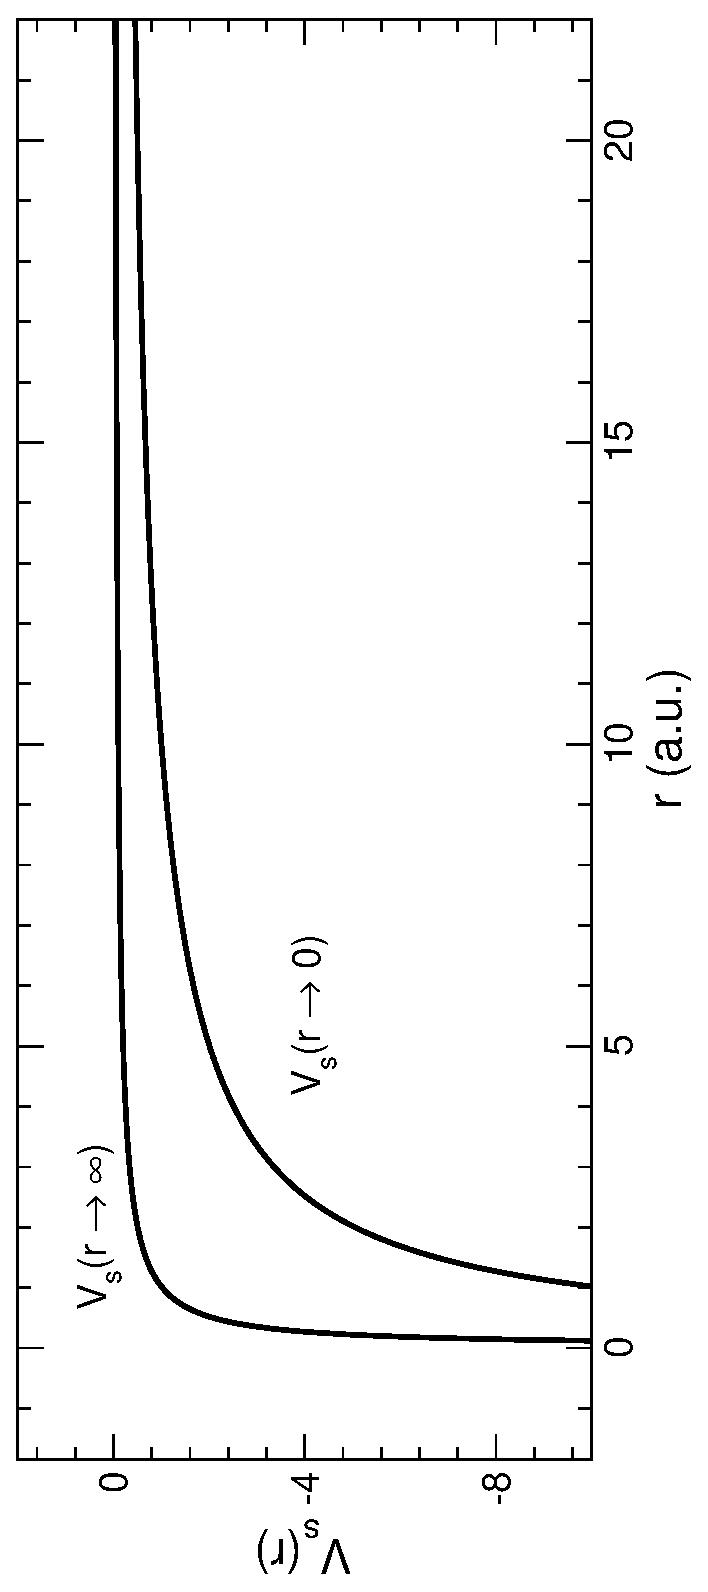
\includegraphics[scale=0.555,angle=-90]{Figures/many_electron/vscreen.eps}
\caption{The right hand sides to the limiting screening potentials defined in equations (\ref{eq:many_vsrzero}) and (\ref{eq:many_vsrinf}) for a test case Ne {\sc i} as a function of the radial distance.  \label{fig:many_vs}}
\end{figure}

Now the major contribution is contained within $H_1$ and the effects of $H_2$ are therefore negligible compared to $H_1$ ($H_2$ << $H_1$). We haven't introduced anything new as the $V_s(r_i)$ will cancel when considering the combined equation (\ref{eq:many_hampert}). This segregation of the Hamiltonian also resembles the form of equation (\ref{eq:many_hbp}), and we can see that the non-relativistic and relativistic contribution represent an unperturbed and perturbed part of the total Hamiltonian respectively. As an initial approximation we disregard the perturbation $H_2$ in equation (\ref{eq:many_H2}) and focus on the central-field Hamiltonian, which is precisely that of (\ref{eq:many_cfham}). At this stage it looks like nothing has changed from our original argument, but now we actually do know the form of $V_s(r_i)$ in its limiting cases, \\
\begin{equation}\label{eq:many_vsrzero}
V_s(r_i \rightarrow 0) = -\frac{Z}{r_i}
\end{equation}
and
\begin{equation}\label{eq:many_vsrinf}
V_s(r_i \rightarrow \infty) = -\frac{Z-N+1}{r_i}     . 
\end{equation}
The right hand sides of these equations can be visualized from Figure \ref{fig:many_vs}, where we sketch both potentials for a neutral case, i.e. $Z=N=10$. The real form of the potential therefore lies somewhere between these two results. Therefore, by considering equation (\ref{eq:many_cfham}), the wavefunction is now separable into a product of $N$, single variable functions for each of the $r_i$.

A similar approach was suggested by Hartree, who had written the total wavefunction for a many-electron problem as the products of the single-electron wavefunctions in equation (\ref{eq:many_fullwave}),
\begin{equation}\label{eq:many_hwave}
\psi(\boldsymbol{r}_1, ..., \boldsymbol{r}_N) = u_1(\boldsymbol{r}_1)u_2(\boldsymbol{r}_2)...u_N(\boldsymbol{r}_N)
\end{equation}
where we have omitted the spin component from the above equation for this analysis and replaced the single-electron wavefunctions by $u_i(\boldsymbol{r}_i)$. The two-body interaction of the electron-electron repulsion can be simplified by assuming the electron moves independently in the field of the remaining electrons, and by spherically averaging this over all angles,
\[
V_i(r_i) = \int V_i(\boldsymbol{r}_i)d\Omega_i = \int \sum_{j\ne i}^{N}\int\frac{|u_j(\boldsymbol{r}_j)|^2}{r_{ij}}  d\boldsymbol{r}_jd\Omega_i.
\]
First we combine the Hamiltonian in equation (\ref{eq:many_ham}) in the approximation of equation (\ref{eq:many_cfham}). Then by considering some wavefunction in the form of equation (\ref{eq:many_hwave}) denoted as Hartree's wavefunction, and upon separation of variables we obtain
	\begin{equation}\label{eq:many_hartree-eq}
	\Big[-\frac{1}{2}\nabla_{i}^2-\frac{Z}{r_i}+V_i(r_i)\Big]u_i(\boldsymbol{r}_i)=E_iu_i(\boldsymbol{r}_i), ~~~~~~~ i=1,...,N
	\end{equation}
where the total energy $E =\sum_i^NE_i$. This particular approach eliminates the complications arising from the electron-electron repulsion and has now become separable into a total of $N$ equations. The functions $u_i(\boldsymbol{r_i})$ are those as defined by equation (\ref{eq:many_fullwave}),
\begin{equation}\label{eq:many_orbitals}
u_{n_il_im_{l_i}m_{s_i}}(\boldsymbol{r}_i) = \frac{1}{r_i}P_{n_il_i}(r_i)Y_{l_im_{l_i}}(\theta_i,\phi_i)
\end{equation}
where we can now express the differential equation from equation (\ref{eq:many_hartree-eq}) in terms of the $P_{n_il_i}(r_i)$ functions, and $R_{n_il_i}(r_i) = \frac{1}{r_i}P_{n_il_i}(r_i)$ has also been introduced. This is useful during the normalization of the radial function and also when solving the differential equations during the numerical integration.

\subsection{Hartree-Fock approximation}\label{ssec:hf}
The Hartree-Fock approximation is based on an independent particle model. The major problem that arises from Hartree's initial assumption is due to the fact that the wavefunction is not antisymmetric in both spin and spatial coordinates in accordance to the interchange of any two electrons. This of course is prohibited due to the effect of the Pauli exclusion principle which is expressed by the following statement,

\protect\textit{``No particles with spin-1/2 may contain identical quantum numbers $n, l, m_l, m_s$ simultaneously.}''

In order to overcome this problem with Hartree's initial wavefunction in equation (\ref{eq:many_hwave}), Fock and Slater proposed a remedy by rewriting $\psi$ in terms of an $N\times N$ dimensional Slater determinant,
	\begin{equation}\label{eq:many_slaterdet}
	\psi(x_1,..,x_N) = \frac{1}{\sqrt{N!}}\left| \begin{array}{cccc}
	u_{\alpha_1}(x_1) & u_{\alpha_2}(x_1) & ... & u_{\alpha_N}(x_1)\\
	u_{\alpha_1}(x_2) & u_{\alpha_2}(x_2) & ... & u_{\alpha_N}(x_2)\\
	\vdots & \vdots & \ddots & \vdots \\
	u_{\alpha_1}(x_N) & u_{\alpha_2}(x_N) & ... & u_{\alpha_N}(x_N) \end{array} \right|.
	\end{equation}
Each $\alpha_i$ denote a set of 4 quantum numbers $\{n_i, l_i, m_{l_i}, m_{s_i}\}$, and $s=1/2$ in accordance with the Pauli exclusion principle. The factor in front of the determinant is to ensure the wavefunction is to be normalized to unity. Without loss of generality, we can assume that the $u_{\beta_i}(\boldsymbol{r})$ are orthonormal to one another, where we have introduced $\beta_i$ to denote the same set of quantum numbers minus the magnetic spin contribution $m_s$. We also relabel $\beta_i \equiv i$ for the equation,
	\begin{equation}\label{eq:many_unorm}
	\Braket{u_i | u_j} = \int u_i^*(\boldsymbol{r})u_j(\boldsymbol{r})d\boldsymbol{r} = \delta_{ij}
	\end{equation}
	where the integral is over all spatial coordinates. Similarly, to account for the magnetic spin term we set $\{m_{s_i}\} \equiv i$, and write
	\begin{equation}\label{eq:many_spinnorm}
	\Braket{\chi_{i} | \chi_{j}} = \sum_{s_z=-1/2}^{+1/2}  \chi_{i}^*(s_z)\chi_{j}(s_z)= \delta_{ij}.
	\end{equation}
The antisymmetric properties arise from the interchange of two rows or two columns, which results in the change of sign of the wavefunction. Also, the wavefunction becomes zero when a set of quantum numbers are equal to each other ($\alpha_i=\alpha_j$).

We can attempt to obtain an optimal Slater Determinant by consideration of the non-relativistic Hamiltonian $H_{\protect\text{NR}}$, from equation (\ref{eq:many_ham}). In the central-field approximation, it was possible to alter the Hamiltonian in such a way to apply perturbation theory. Another approximate method that can be applied whenever it is difficult to find a good description of an unperturbed Hamiltonian is the variational principle. We assume some trial wavefunction with adjustable (variational) parameters and we optimize these parameters until the energy is minimized. The approximate energy functional corresponding to some trial wavefunction $\Phi$ is given by,
	\begin{equation}\label{eq:many_varprinc}
	E_0\leq E[\Phi]= \frac{\Braket{\Phi |H|\Phi}}{\Braket{\Phi |\Phi}}
	\end{equation}
which provides an upper bound to the ground state energy $E_0$. The reason for applying this variational method is to deduce the unknown radial functions, $P_{nl}(r)$.

The minimization procedure is subject to the orthonormality constraints as outlined in equations (\ref{eq:many_unorm}) and (\ref{eq:many_spinnorm}). By taking the trial wavefunction as described in equation (\ref{eq:many_slaterdet}), the functional $E[\psi]$ corresponding to equation (\ref{eq:many_varprinc}) is then made stationary with respect to small variations in the orbitals $u_{\lambda}(x)$ for each $\lambda=\alpha_1, \alpha_2,..., \alpha_N$. By making an infinitesimal change to each of the $u_{\lambda}(x)$ we obtain
	\begin{equation}\label{eq:many_deltaE}
	\delta E-\sum^{\alpha_N}_{\lambda = \alpha_1}\sum^{\alpha_N}_{\mu = \alpha_1}\mathcal{L}_{\lambda\mu}\delta\Braket{u_\mu |u_\lambda}=0,
	\end{equation}
where we have introduced $N^2$ Lagrange multipliers, $\mathcal{L}_{\lambda\mu}$. It is possible to obtain a new diagonal matrix of Lagrange multipliers by performing a unitary transformation on the spin orbitals, $\bar{u}_{\lambda} = \sum_{\mu}U_{\mu\lambda} u_{\mu}$ and therefore $\mathcal{L}_{\lambda\mu} = E_{\lambda}\delta_{\lambda\mu}$, since these Lagrange multipliers form a Hermitian matrix. Assuming that we have selected this unitary transformation from the start, equation (\ref{eq:many_deltaE}) leads to a set of $N$ integro-differential equations, viz, 	
       \begin{equation}\label{eq:many_HF}
	\Big[-\frac{1}{2}\nabla_{i}^2+\mathcal{V}^{(c)}_{\lambda}(x_i)\Big]u^{(c+1)}_\lambda(\boldsymbol{r}_i)=E_\lambda u^{(c+1)}_\lambda(\boldsymbol{r}_i).
	\end{equation}
where $u_{\lambda}^{(c)}(\boldsymbol{r}_i)$ is the spatial part of $u^{(c)}_{\lambda}(x_i)$ at the $c^{\rm th}$ iteration. This has a similar form to that of equation (\ref{eq:many_TISE}) but with a non-local potential $\mathcal{V}^{(c)}(x_i)$ given by,
	\begin{equation}\label{eq:many_HFpot}	
		\begin{split}
	\mathcal{V}^{(c)}_{\lambda}(x_i)=-\frac{Z}{r_i} + & \Bigg[\sum_{\mu}\int u_\mu^*(\boldsymbol{r}_j)\frac{1}{r_{ij}}u_\mu(\boldsymbol{r}_j)d\boldsymbol{r}_j\Bigg]   \\
	- & \Bigg[\delta_{ab}\sum_{\mu}\int u_\mu^*(\boldsymbol{r}_j)\frac{1}{r_{ij}}u_\lambda(\boldsymbol{r}_j)d\boldsymbol{r}_j\Bigg] \frac{u_\mu^{(c)}(\boldsymbol{r}_i)}{u_\lambda^{(c)}(\boldsymbol{r}_i)}.
		\end{split}
	\end{equation}
Now the indices on the Kronecker delta represent the spin quantum numbers, i.e. $a\equiv \{m_{s_a}\}$, and $b\equiv \{m_{s_b}\}$. The equations (\ref{eq:many_HF}) together with the potential in equation (\ref{eq:many_HFpot}) are non-linear, and known as the Hartree-Fock equations. They are solved iteratively at each value for $c > 1$, the first summation in equation (\ref{eq:many_HFpot}) is known as the direct potential, and the second summation accounts for the exchange of electrons and is known as the exchange potential.

\protect{\large{\textit{Self-consistent field method}}}\\
To solve the set of equations (\ref{eq:many_HF}), we briefly outline an iterative procedure known as the self-consistent field method that is applicable in this case. We have already stated that the Hartree-Fock equations (\ref{eq:many_HF}) are not easily solvable, since they amount to a set of integro-differential equations.

The first step in the iterative method starts with an appropriate approximation for the spin-orbitals $u_{\alpha_1}^{(1)}, u_{\alpha_2}^{(1)}, ... ,u_{\alpha_N}^{(1)}$ so that we can then determine $\mathcal{V}^{(1)}$. The integrals are solved for this first iteration and used to determine the set of differential equations in equation (\ref{eq:many_HF}), and therefore solving these equations produces a new set of orbitals, $u_{\alpha_1}^{(2)}, u_{\alpha_2}^{(2)}, ... , u_{\alpha_N}^{(2)}$. The process will terminate when $\mathcal{V}^{(c)}$ is close to $\mathcal{V}^{(c+1)}$ within a pre-specified accuracy, and a similar constraint for the orbitals.

\citet{1974ADNDT..14..177C} represents the radial component of these orbitals by a linear combination of analytical basis functions,
	\begin{equation}\label{eq:many_boundorbs}
	P_{nl}(r)=\sum_{j=1}^kc_{jnl}r^{I_{jnl}}e^{-\eta_{jnl}r}
	\end{equation}
where $c_{jnl}$, $I_{jnl}$ and $\eta_{jnl}$ are coefficients. These are known as Slater-type orbitals (STO's) and describe the general radial form of the wavefunction. The summation grants additional flexibility to their form and the orthonormality conditions from equation (\ref{eq:many_unorm}) also implies that the radial components are orthogonal,
\begin{equation}\label{eq:many_rnlnorm}
\Braket{R_{nl}(r) | R_{\bar{n}\bar{l}}(r)} = \int R_{nl}^*(r)R_{\bar{n}\bar{l}}(r) r^2dr= \int P_{nl}^*(r)P_{\bar{n}\bar{l}}(r) dr =  \delta_{nl,\bar{n}\bar{l}}.
\end{equation}
We will refer to and implement these Hartree-Fock orbitals in future calculations when constructing atomic models. A large tabulation of these are also available in the tables of \citet{1974ADNDT..14..177C}, with details of the calculations therein.

\subsection{The configuration-interaction method}\label{sec:many_ci}
We introduce the configuration-interaction method to account for electron correlation effects, corresponding to a better description of the total wavefunction states. We will therefore investigate how $\Psi_{{\rm HF}}$ can be extended to obtain a better description of these wavefunctions. We begin by considering the angular momentum rules of Russell-Saunders, known as $LS\pi$-coupling outlined in equation (\ref{eq:many_bigLandbigS}).

To account for the electron correlation, we must construct a linear combination of configuration state functions (CSF's). These corresponding atomic state functions (ASF's) then denote some representation of electrons residing in specific orbital shells with quantum numbers $n$ and $l$ that obey the Pauli exclusion principle. The ASF's can be expressed in the following way,
	\begin{equation}\label{eq:many_ciwave}
	\Psi(LS\pi)=\sum_{i=1}^Mc_i\Phi_i(\alpha_iLS\pi)
	\end{equation}
where the CSF's are denoted by $\Phi_i(\alpha_iLS\pi)$, the total wavefunction as $\Psi(LS\pi)$, and $L$, $S$ and $\pi$ being the total orbital and spin angular momentum and the parity of a specific term. These configuration-interaction wavefunctions are typically preferable over the Hartree-Fock description, as $\Psi_{{\rm HF}}$ is often represented by a single CSF. A better approximation of $\Psi(LS\pi)$ will carry an infinite summation, but for practical reasons we terminate with a finite value for $M$. The set of coefficients $\{c_i\}$ are then the weighted contributions from the individual CSF's to the total wavefunction, and $\alpha_i$ represent how the individual electrons $l_i$ and $s_i$ couple together for a total $L$ and $S$. Therefore we require two things; optimized coefficients and CSF's to obtain an accurate total state representation. A similar expression can be written for the fine-structure wavefunction states, $\Psi(J\pi)$ when considering the semi-relativistic corrections of equation (\ref{eq:many_hbp}).\\

\protect{\large{\textit{Optimization of $c_i$'s}}}\\
The first stage is to determine this set of coefficients, $\{c_i\}$. By considering the variational principle in equation (\ref{eq:many_varprinc}) again, we can keep the $\Phi$'s fixed (which we still do not know) while the coefficients constitute the variational parameters. We also perform the minimization subject to the orthonormality of the total $\Psi(LS\pi)$. Assuming $\Psi(LS\pi)$ in equation (\ref{eq:many_ciwave}) as our total wavefunction for a particular state, together with the variational principle, we can obtain the following equation,
\begin{equation}\label{eq:many_optc}
\delta \Big[ \sum_i \sum_j c_ic_j\Braket{\Phi_i | H | \Phi_j} - E_i\Big(\sum_i \sum_j c_ic_j\Braket{\Phi_i | \Phi_j} -1\Big)\Big] = 0.
\end{equation}
Here we have introduced $M$ Lagrange multipliers, labelled as $E_i$. The CSF's constitute an orthonormal set, similarly to the ASF's, and this variational principle reduces equation (\ref{eq:many_optc}) to an eigenvalue problem,
\begin{equation}\label{eq:many_hij}
\sum_j^{M}c_j(\Braket{\Phi_i | H | \Phi_j} - E_i\delta_{ij}) = 0 ~~~ i=1,...,M.
\end{equation}
Therefore, the eigenvector components $\{c_i\}$ also represent the contribution of the diagonalized matrix elements $\Braket{\Phi_i | H | \Phi_j}$ for a particular ASF. This ASF is also categorized by its Lagrange multipliers $E_i$, as they also correspond to their energy eigenvalues.\\

\protect{\large{\textit{Optimization of $\Phi_i$'s}}}\\
We have defined our basis expansion to have a total of $M$ CSF's to describe a particular wavefunction, $\Psi(LS\pi)$. The corresponding set of eigenvalues for a basis set of size $M$ can be easily ordered in the following way,
\begin{equation}\label{eq:many_hyll1}
E_1^{(M)} < ... < E_M^{(M)}.
\end{equation}
Then by including an additional CSF, $\Phi^{(M+1)}$, we can also order the corresponding $E_i^{(M+1)}$ in a similar fashion to equation (\ref{eq:many_hyll1}). The Hylleraas-Undheim theorem states that we can interleave these as follows,
\begin{equation}\label{eq:many_hyll2}
 ... < E_{i-1}^{(M)} < E_i^{(M+1)} < E_i^{(M)}  < E_{i+1}^{(M+1)} < ...
\end{equation}
It is not hard to see from equation (\ref{eq:many_hyll2}) that the inclusion of more CSF's indicates some convergence of the basis set. This is obviously not possible to implement in practice, but it is clear that if $M \rightarrow \infty $, then we obtain an upper bound for the exact energy,
\[
E_i^{(M)} > E_i^{(exact)}
\]
which provides a minimization constraint for all excited states $i$. It should also be mentioned that for the sketched proof above, we have written $E_i$ to represent the $i^{th}$ lowest eigenvalue for this choice of $M$ CSF's.

\section{Transition probabilities}\label{sec:many_transition}
Until now we have been focused on obtaining multiple ways to describe the wavefunctions for as many states as possible. The next step is to consider what happens when some transition between two states takes place. We begin by considering three important mechanisms below.\\

\protect{\large{\textit{Spontaneous emission}}}\\
Suppose that we have a total of $N_j(t)$ atoms at a particular time $t$, where the subscript represents the number in that state $\Ket{j}$. Then the rate of change to some other sate $\Ket{i}$ can be written as,
\[
\frac{dN_j(t)}{dt} = -N_j(t)A_{j\rightarrow i}.
\]
This equation can be extended to consider the total spontaneous emission
\begin{equation}\label{eq:many_spontaneous}
\frac{d N_j(t)}{dt} = - N_j(t)\sum_i^{j-1}A_{j \rightarrow i},
\end{equation}
which is solvable for $N_j(t)$. The summation in equation (\ref{eq:many_spontaneous}) allows for decay to any levels that lie energetically below the current occupancy. Due to the conservation of energy, the spontaneous emission from an upper state $(j)$ to a lower state $(i)$ simply means that the system loses energy in the form of a photon $h\nu_{ji}$, so the change in energy is therefore subject to $h\nu_{ji} = E_j - E_i$. The subscripts on $\nu$ will often be omitted but are included for clarity here. Another useful property is to consider the mean lifetime of $\Ket{j}$ before it radiatively decays, and is defined as
\[
\tau_j = \frac{1}{\sum_i^{j-1}A_{j \rightarrow i}}
\]
which is just the mean time it takes for some state $\Ket{j}$ to decay (i.e. lose energy) to any of the remaining $(j-1)$ states that lie energetically below it.\\

\protect{\large{\textit{Stimulated emission $\&$ absorption}}}\\
We must also account for external influences acting on the system that can alter the internal energy. The first that we describe is known as stimulated emission, $B_{j \rightarrow i}$, which resembles the process of spontaneous emission. The difference is that the system is provided with some form of energy, but enough energy is still lost for a decay to a lower level to occur. The second mechanism is stimulated absorption, where the system gains an amount of energy and therefore excited states can be reached, and is written similarly as $B_{i \rightarrow j}$. This can occur due to the presence of an isotropic, external radiation field, and we assume that the energy per unit volume of this field is $\rho(\nu)d\sigma$. Therefore we can summarize the rate that atoms in state $\Ket{j}$ are stimulated to a lower level $\Ket{i}$ is described by the following,
\begin{equation}\label{eq:many_semission}
\frac{d N_j(t)}{dt} = - B_{j \rightarrow i}N_j(t)\rho(\nu_{ji}).
\end{equation}
Then the absorption of atoms in a state $\Ket{i}$ to a higher state $\Ket{j}$ are given by the rate,
\begin{equation}\label{eq:many_sabsorption}
\frac{d N_i(t)}{dt} = - B_{i \rightarrow j}N_i(t)\rho(\nu_{ji}).
\end{equation}
By assuming detailed balance, we must have equality between the rate of absorption and stimulated plus spontaneous emission between two states. This allows us to relate the following quantities in equations (\ref{eq:many_spontaneous}), (\ref{eq:many_semission}) and (\ref{eq:many_sabsorption}) as
\begin{equation}\label{eq:many_AwithBB}
N_j(t)(A_{j \rightarrow i}+B_{j \rightarrow i}\rho(\nu_{ji})) = B_{i \rightarrow j}N_i(t)\rho(\nu_{ji}).
\end{equation}
By applying Plank's law for $\rho(\nu_{ji})$, and Boltzmann's equation for level populations, we find that
\begin{equation}\label{eq:many_boltz}
\frac{N_j(t)}{N_i(t)} = \frac{g_j}{g_i}e^{-(E_j-E_i)/kT},
\end{equation}
where $k$ is the Boltzmann constant and $T$ is the temperature, it is now possible to rearrange equation (\ref{eq:many_AwithBB}). The stimulated coefficients can also be related to the absorption coefficients by a ratio of statistical weights,
\begin{equation}\label{eq:many_BtoB}
B_{j \rightarrow i} = \frac{g_i}{g_j}B_{i \rightarrow j}.
\end{equation}
We have introduced the statistical weight of a particular level the first time, and we will use this notation throughout the thesis. We define,
\begin{equation}\label{eq:many_statweight}
g_k = \left\{
  \begin{array}{lr}
     (2L_k+1)(2S_k+1)\\
    (2J_k+1)
  \end{array}
\right.
\end{equation}
as be the weight of some state $\Ket{k}$. This weighting is due to the degeneracy in $L$, $S$, and $J$, for example $-L\leq M_L\leq L$. 

\section{Oscillator strengths}\label{sec:many_oscillator}
Another useful quantity is known as the oscillator strength, which measures the strength of absorption between a lower state $\Ket{i}$ to a high lying state $\Ket{j}$. This newly defined oscillator strength can be rewritten in terms of the absorption coefficient,
\begin{equation}\label{eq:many_fwithb}
f_{i\rightarrow j} = \frac{\mu}{\pi e^2}h\nu_{ji}B_{i\rightarrow j},
\end{equation}
where $\mu$ and $e$ are the reduced mass and electronic charge of the electron respectively. In atomic units these quantities are set to unity. This allows us to obtain a relationship between the emission oscillator strength and absorption oscillator strength by substituting equation (\ref{eq:many_BtoB}) into equation (\ref{eq:many_fwithb}),
\[
f_{i\rightarrow j} = -\frac{g_j}{g_i}f_{j\rightarrow i}.
\]
Also from equation (\ref{eq:many_fwithb}), the relationship with the absorption coefficient $B_{i \rightarrow j}$ provides another useful relationship between the transition probability and oscillator strength by applying equation (\ref{eq:many_AwithBB}) and equation (\ref{eq:many_BtoB}) to obtain
\begin{equation}\label{eq:many_fijandaij}
f_{i\rightarrow j} = \frac{g_j}{g_i}\frac{\mu c^3}{8\pi^2 e^2 \nu_{ji}^2}A_{j\rightarrow i}.
\end{equation}
Since $A_{j \rightarrow i}$ is in units of $t^{-1}$ (and $f_{i\rightarrow j}$ is dimensionless), then this direct proportionality indicates that for transitions that are more likely to occur, then the strength of the line increases, as would be expected. Since the transition probability is referred to more commonly as a rate, we must consider a time-dependent wavefunction expansion to express such transitions between states. This is introduced through an external radiation field, where one such example can be written as
\[
\boldsymbol{A_0}\cos(\omega t - \boldsymbol{k} \cdot \boldsymbol{r})
\] 
for an electric dipole transition. $\boldsymbol{A_0}$ is the amplitude of the radiation field and the magnitude of $\boldsymbol{k}$ is defined as the wavenumber,
\begin{equation}\label{eq:many_wavenumberk}
|\boldsymbol{k}| = k = \frac{2\pi}{\lambda_{ji}}.
\end{equation}
To apply time-dependent perturbation theory, we can think of the radiation field as a small perturbation, and then expand the unperturbed part of the total wavefunction as
\[
\Psi = \sum_j c_j(t) \psi_j e^{-iE_jt},
\]
together with the corresponding absorption coefficient,
\begin{equation}\label{eq:many_bstrength}
B_{i\rightarrow j} = \frac{2}{3}\frac{c^2 \pi}{h^2 \nu_{ji}^2} \Bigg | \Braket{\psi_j | \frac{e}{\mu c}\sum_m\boldsymbol{p}_me^{i\boldsymbol{k} \cdot \boldsymbol{r}} | \psi_i} \Bigg |^2.
\end{equation}
The summation is carried over each electron in the system and $\boldsymbol{p}_m$ corresponds to the momentum of electron $m$. We already have a relationship between $B_{i\rightarrow j}$ and $f_{i\rightarrow j}$, so finding an expression for the oscillator strength is straight forward, but the difficulty arises due to the form of the exponential function. We can relax this complication by applying a Taylor expansion the function resulting in the dipole approximation,
\[
e^{i\boldsymbol{k} \cdot \boldsymbol{r}} = 1 + i\boldsymbol{k} \cdot \boldsymbol{r} + ... \approx 1.
\]
This seems like a big assumption and simplification, but it is quite reasonable as $\langle \boldsymbol{k} \cdot \boldsymbol{r} \rangle \ll 1$. The magnitude of $\boldsymbol{r}$ is typical of a few angstroms, compared to the magnitude of $\boldsymbol{k}$ defined in equation (\ref{eq:many_wavenumberk}), which contains a $1/\lambda_{ji}$ term where $\lambda_{ji}$ is typical of a few hundred to many thousand angstroms. Therefore by combining equation (\ref{eq:many_bstrength}) and equation (\ref{eq:many_fwithb}) then we can write the oscillator strength as
\begin{equation}\label{eq:many_osc_vel}
f_{i\rightarrow j}^v = \frac{2}{3}\frac{1}{(E_j-E_i)} \Bigg | \Braket{\psi_j | \sum_m\boldsymbol{\nabla}_m | \psi_i} \Bigg |^2.
\end{equation}
in atomic units, and $h\nu_{ji} = E_j - E_i$. This is known as the velocity form of the oscillator strength, but other forms do exist. The length form can be obtained using the commutation relation with the Hamiltonian, $[\boldsymbol{r},H] = i\boldsymbol{p}$. By substitution of this into equation (\ref{eq:many_osc_vel}) we find that
\begin{equation}\label{eq:many_osc_len}
f_{i\rightarrow j}^l = \frac{2}{3}(E_j-E_i) \Bigg | \Braket{\psi_j | \sum_m\boldsymbol{r}_m | \psi_i} \Bigg |^2.
\end{equation}
In practice we would hope that these quantities are extremely similar for exact wavefunctions, $f_{i\rightarrow j}^l =f_{i\rightarrow j}^v$, but we have already seen that we need to truncate the basis expansion in equation (\ref{eq:many_ciwave}) which has an effect on the results. A good measure and check is to note the ratio between these two different definitions of the oscillator strengths should be equal to one. However, just because they are close or exact, does not necessarily infer correctness, and therefore a systematic analysis of the oscillator strengths must be carried out. One approach is to consider the convergence for an increasing size of the configuration-interaction expansion of the total wavefunction. Another reason is that the commutation only applies to local potentials, but it is generally considered as an acceptable approximation to make.

In proceeding Chapters we apply the decay rates $A_{j \rightarrow i}$ when considering the theory required for spectral modelling. When we substitute the relationship between these rates and the oscillator strengths from equation (\ref{eq:many_fijandaij}) into equation (\ref{eq:many_osc_len}), an $(E_j-E_i)^3$ appears in the numerator. The calculated energy levels are often different from observation or experiment, so an adjustment can be made to the $A$-values. They are scaled through the factor,
\begin{equation}\label{eq:many_ascale}
\Bigg(\frac{\Delta E^{{\rm expt}}}{\Delta E^{{\rm theor}}}\Bigg)^\eta
\end{equation}
where $\eta = 3$ as discussed above for electric or magnetic dipole transitions. However, after some analysis, it can be found that $\eta=5$ for electric or magnetic quadrupole transitions. Therefore, subtle differences in energies can result in significant scaling of the $A$-values. 

\section{{\sc civ3}}\label{sec:many_civ3}
The method of configuration-interaction discussed in Section \ref{sec:many_ci} is implemented into the computer package {\sc civ3} developed by \citet{1975CoPhC...9..141H} to obtain descriptions for atomic wavefunctions. In this Section we will briefly outline some of the major processes that can be computed and the general computation required by the code.

The Hamiltonian matrix defined in equation (\ref{eq:many_hij}) are constructed by projecting the target states onto it, and using the definition of the non-relativistic Hamiltonian in equation (\ref{eq:many_hbp}) together with equation (\ref{eq:many_TV1V2}) we can write,
\[
\begin{split}
\Braket{\Phi_i | H_{NR}^{N} | \Phi_j} = &\Braket{\Phi_i | T + V_1 + V_2 | \Phi_j}\\
= &\Braket{\Phi_i | T + V_1| \Phi_j} +\Braket{\Phi_i | V_2 | \Phi_j}.
\end{split}
\]
Then by considering equations (\ref{eq:many_T}) and (\ref{eq:many_V1}), we can write the radial matrix elements as,
\[
\Braket{\Phi_i | T + V_1| \Phi_j} = \sum_{kk'}x_{ij}(k,k')\Braket{P_{n_kl_k}| -\frac{1}{2}\frac{d^2}{dr^2}-\frac{Z}{r}+\frac{l_k(l_k+1)}{2r^2}| P_{n_{k'}l_{k'}}}\delta_{l_kl_{k'}}
\]
where the radial part of the $\Phi_i$'s have been expressed in terms of their one-electron components using the $P_{nl}$ functions defined in equation (\ref{eq:many_orbitals}). $k$ and $k'$ are introduced to represent the electron in particular subshells of $\Phi_i$ and $\Phi_j$ respectively. These correspond to one-electron radial integrals, and the evaluation of these coefficients $x_{ij}(k,k')$ have been detailed by \citet{1974CoPhC...7..318H}. Similarly, we can write
\[
\Braket{\Phi_i | V_2| \Phi_j} = \sum_{kmk'm'}\sum_{d}y_{ij}(km,k'm',d)R^d(nl_k,nl_m;nl_{k'},nl_{m'})
\]
where $m$ and $m'$ also represent an electron in a particular subshell of $\Phi_i$ and $\Phi_j$ respectively. These are known as the two-electron radial integrals where the coefficients $y_{ij}(kmk'm',d)$ can be written in terms of Racah algebra \citep{1965PhRv..140...67F} and determined from the program of \citet{1971CoPhC...2..180H}. The radial functions are expressed as STO's defined by equation (\ref{eq:many_boundorbs}). Their corresponding integrals $R^d$ are transformed to Slater integrals and solved analytically, which have numerous advantages as they can be computed exactly. The angular integrals expressed in terms of the Spherical Harmonics are also evaluated here by employing the same convention of Racah algebra.

Eigenenergies are obtained by diagonalizing the Hamiltonian matrix, and the eigenvector components represent the coefficients $c_i$ in equation (\ref{eq:many_ciwave}). It is possible to optimize the STO coefficients by minimizing select eigenvalue functionals, or combinations of eigenvalues. 

Configuration-interaction wavefunctions are constructed by including (for how to select these, see Section \ref{sec:many_config} configurations into the expansion. There are numerous tests and indicators for checking whether the wavefunctions actually produced meaningful results. The measurables defined by oscillator strengths and transition probabilities in Sections \ref{sec:many_transition} and \ref{sec:many_oscillator} respectively can be produced as we now have a multiple state system. These quantities together with the energy eigenvalues can be compared with observed or experimentally determined results for an indication of accuracy from these theoretical predictions. 

\section{{\sc grasp0}}\label{sec:many_grasp0}
Another extremely useful approach is by considering the relativistic structure code {\sc grasp0}, and in this Section we will outline some of the major functions and differences compared with {\sc civ3}. However, we ultimately require accurate descriptions for the wavefunction expansions, and both packages produce meaningful results if implemented correctly. Since the computations are based on various numerical methods, approximations, and theory, it is useful to perform and provide a wide variety of results through different theoretical approaches if possible. 

There are a few major and defining features that set the two packages apart. The first is that {\sc grasp0} is based on the Dirac equation, where the Hamiltonian operator is similar to equation (\ref{eq:many_TISE}), which also considers the kinetic and potential energy to describe the total energy of the system and can be written as
\begin{equation}\label{eq:many_dirac_ham}
H^N_{\text{D}} = \sum_{k=1}^N-ic\boldsymbol{\alpha}\nabla_k +(\boldsymbol{\beta}-1)c^2 - \frac{Z}{r_k} + \sum_{k<j=1}^N\frac{1}{r_{kj}}.
\end{equation}
$\boldsymbol{\alpha}$ and $\boldsymbol{\beta}$ are simply $4\times 4$ Pauli spin matrices, and $c$ is the speed of light. Likewise, there are perturbative corrections that can be applied to this Hamiltonian to account for additional effects that we will not define here. These include Breit interactions, Quantum electrodynamic effects and transverse photon effects. 

The wavefunctions are still configuration-interaction wavefunctions taking the form of equation (\ref{eq:many_ciwave}), but using the notation of $\Psi(J\pi)$ so that commutation between $\boldsymbol{J}^2$ and $\boldsymbol{J}_z$ with equation (\ref{eq:many_dirac_ham}) is satisfied. The second major difference is that the target states $\Phi(\alpha_iJ\pi)$ are no longer products of one-electron orbitals, but represented by one-electron Dirac spinors of the form,
\begin{equation}\label{eq:many_diracwave}
\phi = \left( \begin{array}{c}
	\phi_{L}\\
	\phi_{S} \end{array} \right) = \frac{1}{r}\left( \begin{array}{c}
	\xi_{\kappa,m_j}(\theta,\psi)\mathcal{P}_{\kappa}(r)\\
	i\xi_{-\kappa,m_j}(\theta,\psi)\mathcal{Q}_{\kappa}(r) \end{array} \right) .
\end{equation}
$\mathcal{P}_{\kappa}(r)$ now represents the large component and $\mathcal{Q}_{\kappa}(r)$ the small component of the wavefunction. The spinors defined by $\xi_{\kappa,m_j}(\theta,\psi)$ can be one or two products of Clebsch-Gordan coefficients with the spherical harmonics. We have also introduced the quantum number $\kappa$ here which represents the pair $(l,j)$ of an electron such that,
\begin{equation}\label{eq:many_kappacoupling}
\kappa = \left\{
  \begin{array}{lr}
     -(l+1) ~~~~{\rm for}~~~~~~  j = l + \frac{1}{2}\\
    ~~~~~ l ~~~~~~~~~{\rm for}~~~~~~  j = l - \frac{1}{2}
  \end{array}
\right.
\end{equation}
We also note that since $j>0$, so there is only one $\kappa$ value that corresponds to $l=0$. The variational method is invoked again to obtain two sets of coupled first order differential equations, i.e. one for the large component and one for the small component that will be discussed in Chapter \ref{cha:rmatrix}. An iterative procedure is then used to solve the set of equations to obtain the optimized radial functions and coefficients (eigenvector components of the diagonalized Hamiltonian). 

\section{Alternative computer packages}\label{sec:many_alt}
We have detailed just two sets of computer codes that we heavily rely on in this work, but there are other well established and documented codes that exist. In this Section we will provide a short overview and description of three different approaches, the Cowan code, {\sc mchf}, and {\sc autostructure}. While we do not directly implement these packages during our calculations, we compare with existing work that has. We can therefore understand the main differences between the optimization procedure and orbital description of other major computer codes.

\subsection{The Cowan code}\label{ssec:many_cowan}
The Cowan code \citep{1981tass.book.....C} uses a variety of model potentials to drastically simplify the calculations, and a central-field type Hamiltonian is incorporated to describe the total energy of the system. Modifications are then applied to the Hartree-Fock equations to alleviate some of the restrictions from the complicated potential, $\mathcal{V}$ which is currently detailed in equations (\ref{eq:many_HF}) and (\ref{eq:many_HFpot}). The Hartree-Fock-Slater approach represents the electron orbitals as plane waves, and another modification is known as Hartree-statistical-exchange, where the exchange term of the potential is altered, and additional corrections are applied to account for the one body perturbative terms.

The remainder of the computation follows as normal, where trial radial wavefunctions are chosen and optimized using the self-consistent field method by selecting an appropriate form for the central-field potential function. In summary, the Cowan code attempts to save on computation by simplifying the equations needed to be solved through the usual Hartree-Fock approach.

\subsection{Multi-configuration Hartree-Fock - {\sc mchf}}\label{ssec:many_mchf}
This package developed by \citet{1991CoPhC..64..369F} has many similarities with {\sc civ3}. The wavefunction expansions are still determined using the variational principle (\ref{eq:many_varprinc}), and the Hamiltonian operator implemented is exactly the same, with the perturbative corrections of (\ref{eq:many_bp1}), (\ref{eq:many_bp2}) and (\ref{eq:many_bp3}). The configuration-interaction coefficients are obtained by using the same technique as {\sc civ3} by diagonalizing the Hamiltonian matrix.

Since {\sc civ3} already knows the analytic form of the radial functions in equation (\ref{eq:many_boundorbs}), the variational principle can be applied directly during the optimization process. In {\sc mchf}, the variational principle is still implemented, but to produce a new set of integro-differential equations, where the solutions are the unknown radial functions. A radial grid with logarithmic increments is established and the equations are solved using numerical techniques by applying the self-consistent field method. The logarithmic grid is extremely beneficial, as the radial form closest to the nucleus is the most challenging, and for large $r$ we know this tends to zero.

There is another similar method to the theory behind {\sc mchf} known as {\sc mcdf} from \citet{1970AdPhy..19..747G} and \citet{1980CoPhC..21..207G}, which is the multi-configuration Dirac-Fock suite of codes. It is more closely related to {\sc grasp0}, and the equations and descriptions for the wavefunctions are the defining differences between it and {\sc mchf}. The equations (\ref{eq:many_dirac_ham}) and (\ref{eq:many_diracwave}) are considered for this approach instead.

\subsection{{\sc autostructure}}\label{ssec:many_auto}
This computer code is a major revision of its predecessor {\sc superstructure} developed originally by \citet{1974CoPhC...8..270E}. It has since been renamed to {\sc autostructure} which was first introduced by \citet{1986JPhB...19.3827B}, and is constantly undergoing major revisions, such as the inclusion of the two-body Hamiltonian operators by \citet{1997JPhB...30....1B}. The code is extremely flexible, and various bound orbital descriptions such as those from {\sc civ3} or {\sc mchf} can be implemented. However, the code can generate a set of orbital parameters through a Thomas-Fermi-Dirac model potential, $V^{\lambda_{nl}}(r)$ for each $nl$. Therefore, a different potential function is defined for each $nl$ and these scaling parameters $\lambda_{nl}$ are determined from the variational principal through a minimization procedure. {\sc autostructure} also has the ability to incorporate a continuum orbital, and therefore additional processes can also be calculated.

\section{Selecting configurations}\label{sec:many_config}
For a given state of the Hartree-Fock approximation, we denote the energy and wavefunction as $E_{\protect\text{HF}}$ and $\Psi_{\protect\text{HF}}$ respectively. However, these are just approximations to the exact energy and wavefunction which we shall note by $E_{\protect\text{ex}}$ and $\Psi_{\protect\text{ex}}$ respectively. This is a very powerful and accurate approximation, but we can write the correction to the exact energy as,
	\begin{equation}\label{eq:many_correlatione}
	E_{\protect\text{corr}}=E_{\protect\text{ex}}-E_{\protect\text{HF}}
	\end{equation}
where $E_{\protect\text{corr}}$ is known as the correlation energy. The remainder of this Section considers how to reduce the difference between the calculated energy and the exact energy, $E_{\protect\text{ex}}$.

Now we have the important ingredients to begin our calculations, and definitions for multiple, useful quantities that can be `easily' determined if the computer codes are utilized correctly. One of the last points to discuss is what configurations are generally required to be incorporated into the calculations. For this, we shall consider a typical test case of B {\sc i}, where the ground state can be written in spectroscopic notation as 1s$^2$2s$^2$2p $^2$P$^{{\rm o}}$ ($N=5$). The configuration can be classified by three components.\\

\protect{\large{\textit{Internal correlation}}}\\
The internal correlation is defined to be the correlation which can be obtained by using the Hartree-Fock orbitals for the $nl$ values that are occupied, so in our case, $n=2$ and $l = 1$. We recall that the parity must be conserved, and is obtained by simply summing over the individual orbital momentum of each electron ($=1$, therefore odd states). If the only states we are concerned with are those that result in $^2$P$^{{\rm o}}$ states, then we could consider the following as internal correlation configurations; 1s$^2$2p$^3$, 2s$^2$2p$^3$, or 2p$^5$. Generally speaking, if we are looking at more complicated systems, the first would be the most beneficial to include. The core is usually kept closed as these electrons are more tightly bound, and the transitions are amongst non-core orbitals. The mathematical interpretation is that the $c_i$ for these configurations are negligible or contribute little to the energy differences of the state.\\

\protect{\large{\textit{Semi-internal correlation}}}\\
This type of correlation is defined by considering 4 electrons from Hartree-Fock, or from its set of orbitals and one electron outside of this set. Therefore a direct replacement of the 2s to an orbital outside this set would result in configurations of the form 1s$^2$2s2p3s, or 1s$^2$2s2p3d. Another approach is to consider a multi-reference set and include configurations that we define as internal corrections such as 1s$^2$2p$^3$. This leads to configurations such as 1s$^2$2p$^2$3p, or 1s$^2$2p$^2$4p.\\

\protect{\large{\textit{External correlation}}}\\
The final is the more obvious, and basically consists of everything else that would complete the entire basis set, i.e. no more than 3 electrons residing in the Hartree-Fock set and the remaining in orbitals outside. 

There are many ways to investigate the importance of including these forms of correlation. The most precise way is to look at the eigenvector components $\{c_i\}$ themselves to see if they change and by how much. Another way is to survey the atomic data that has been calculated such as convergence of transition probabilities or energy eigenvalues, and how they compare with other works. The oscillator strengths should also converge to a ratio of one for their length and velocity forms. A combination of all these factors give indications of which contributions are most important, and those that have little to no effect yet result in a larger calculation.

\section{Selection rules}\label{sec:many_selection}
We have already stated that transitions between two states are of extreme importance for determining multiple processes. So far it has only been mentioned that these are possible to compute and that they produce useful quantities. However, only transitions between specific angular momenta are possible; this comes from a direct consequence of the radiation field considered. We have considered electric-dipole (E1) transitions in deriving the respective form for the oscillator strengths and $A$-values, however there are other types of transitions that exist. We can also have magnetic dipole (M1), and electric/magnetic quadrupole (E2/M2). Assuming that we have a transition from $\psi_i\rightarrow\psi_f$, then the following rules are to be adhered,

\begin{itemize}
\item{An E1 and M2 transition is only possible when there is a change in parity between $\psi_i$ and $\psi_f$, while there is no change in parity for E2 and M1 transitions.}
\item{The difference of total orbital angular momentum between $L_i$ and $L_j$ cannot exceed a difference of 1 for E1 and M1 transitions, and 2 for E2 and M2 transitions. So when considering E1 and M1 transitions, $|L_i - L_j|\leq 1$, therefore an angular momentum of $L_i=2$ results in the allowed values of $L_j=1,2,3$. The only limitation to this rule is that the transition for $L_i=L_j=0$ is not possible for E1 and M1, and $L_i=L_j=\{0,1\}$ for E2 and M2.}
\item{The final rule is that the total spin angular momentum $S$, must remain constant throughout between $\psi_i$ and $\psi_f$. Therefore $S_i=S_j$ must necessarily hold for all types of transitions.}
\end{itemize}
If all three above hold then the transition is said to be allowed, but if any fail for a particular case then the transition is referred to as forbidden. However, there is one extra condition when considering an $LSJ$-coupling scheme.
\begin{itemize}
\item{The total angular momentum between $J_i$ and $J_j$ cannot exceed a difference of 1 for E1 and M1 transitions, and 2 for E2 and M2 transitions. Again, we have that $J_i=J_j=0$  is not possible for E1 and M1, $J_i=J_j=\{0,1\}$ and $J_i=J_j=1/2$ for E2 and M2.}
\end{itemize}
We can now replace the second and third points by this final point, but the rules for parity still hold. This last point stresses the importance of including relativistic effects into our calculations. Transitions that are normally considered forbidden in $LS$ coupling are in fact allowed due to the total angular momentum coupling and are referred to as intercombination lines. We can consider the example of
\[
1{\rm s}^22{\rm s}^2 ~^1{\rm S}_{0} \rightarrow 1{\rm s}^22{\rm s}2{\rm p} ~^3{\rm P}_1^{\rm o}
\]
and due to the $\Delta S>0$, then this transition is forbidden in $LS\pi$ coupling. However, because the $^3$P$^{\rm o}_{1}$ mixes with $^1$P$^{\rm o}_{1}$, then this transition is possible in an $LSJ\pi$ coupling scheme.

%----------------------------------------------------------------------------------------



% Chapter 1

\chapter{The $R$-matrix method} % Main chapter title

\label{cha:rmatrix} % For referencing the chapter elsewhere, use \ref{Chapter1} 

\lhead{Chapter 3. \emph{The $R$-matrix method}} % This is for the header on each page - perhaps a shortened title

%----------------------------------------------------------------------------------------

\section{Photon and electron interactions}\label{sec:cross}
In this Chapter we will focus first on covering the basic concepts behind the atomic processes of photoionization and electron-impact excitation. We will extend these basic and informal definitions and incorporate them into the $R$-matrix method which follows in the next Section.

We consider some atomic system denoted by $X_i^{q+}$, which is in some initial state $i$. This system can then absorb a photon with enough energy to ionize $X_i^{q+}$ to leave it in the ground state or some excited state, $X_f^{(q+1)+}$ with the ejection of an electron into the continuum. This photoionization process can now be written in the following way,
\begin{equation}\label{eq:rmat_basicphoto}
\begin{split}
& ~~~~~~~~~~~~~~ \tiny{\circled{1}}\\
& h\nu+ X_i^{q+} \rightarrow X_f^{(q+1)+} +e^-\\
& ~~~\tiny{\circled{2}}\searrow ~~~~~~~~~~~~~~~~~\nearrow \tiny{\circled{2}} \\
& ~~~~~~~~~~~~(X_y^{q+})^*
\end{split}
\end{equation}
where $X_i^{q+}$ has some eigenenergy $E_i$, in its initial state with corresponding eigenstate $\Psi_i$. Likewise, $X_f^{(q+1)+}$ is left in some final state with corresponding eigenenergy $E_f$. Finally, the electron that is ejected from the system, otherwise known as a photoelectron, leaves with some momentum $\boldsymbol{k}_f$. The process along the top arrow 1) in equation (\ref{eq:rmat_basicphoto}) is known as direct photoionization. However, following the secondary route 2), we can temporarily excite $X_i^{q+}$ into some autoionization state $y$ before the ejection of the electron. We must also adhere to the conservation of energy, so we can then write the following equation,
\[
h\nu+E_i=\frac{1}{2}k_f^2+E_f.
\]
where we have set the mass of the electron $m_e=1$.

The next important process that we will be covering in this thesis is known as electron-impact excitation and it can also be written informally as,
\begin{equation}\label{eq:rmat_basicelectron}
\begin{split}
& ~~~~~~~~~~~~~~ \tiny{\circled{1}}\\
& e^- + X_i^{q+} \rightarrow X_f^{q+} + e^-.\\
& ~~~\tiny{\circled{2}}\searrow ~~~~~~~~~~~~~~\nearrow \tiny{\circled{2}} \\
& ~~~~~~~~~(X_y^{(q-1)+})^*
\end{split}
\end{equation}
The electron can therefore transfer its energy to make some transition from a lower ($i$) to higher ($f$) energy state as described before for the photoionization process, and is similarly referred to as its 1) direct excitation pathway. Likewise, the electron can become temporarily bound in a resonant state and this is known as the 2) indirect pathway.


\section{$R$-matrix theory}\label{sec:rmatrix}
Despite the non-relativistic $R$-matrix method being implemented first to describe nuclear interactions \citep{1947PhRv...72...29W}, and furthermore generalized to a relativistic approach by \citet{1948PhRv...73.1463G}, it has since been applied to atomic processes based on the fundamental concepts from scattering theory. Due to the substantial complexity of the computer codes, its capabilities are ever changing and improving. To begin this Chapter, we note some of the major advancements in the field that has allowed us to perform such sophisticated calculations. 

It had become clear that these interactions could be understood by the $R$-matrix method by \citet{1968AdAMP...4..173B}. The theory was then first implemented to consider electron-atom collisions \citep{1971JPhB....4..153B}, and resulted in the first $R$-matrix codes in $LS\pi$ coupling \cite{1974CoPhC...8..149B}. The theory of photoionization was then described in the $R$-matrix framework by \citet{1975JPhB....8.2620B}. Further modifications based on the Breit-Pauli Hamiltonian operators are detailed by \citet{1980JPhB...13.4299S}, resulting in the extension to the {\sc bp} suite of codes \citep{1982CoPhC..25..347S, 2001JPhB...34.4455M}. Many of the routines were based on the computer package {\sc civ3} when treating the target state problem, due to its similarities. A general overview can be obtained in the book of \citet{2011rmta.book.....B} and technical documents describing the important routines and variables are presented by \citet{1995CoPhC..92..290B}. However, this is not the extent of its capabilities, further extensions for calculating polarizabilities \citep{1973JPhB....6..945R}, and to include molecular systems \citep{1977JPhB...10.2497B} have also been considered.

The {\sc darc} suite of relativistic codes were based originally on {\sc grasp} \citep{1979CoPhC..17..149G}, and provides an alternative procedure for heavier systems. The theory has been considered by \citet{1975JPhB....8.2327C} and solutions for the asymptotic equations can be obtained by \citet{1994CoPhC..83..215Y}.

This is not the end of the story for $R$-matrix theory, and the above are just a handful of publications amongst many others. These underlying techniques have been implemented to consider a range of other approaches such as the B-splines (code - {\sc bsr}) method by \citet{2006CoPhC.174..273Z} which employs a non-orthogonal basis, or the intermediate-coupling frame transformation method (code - {\sc icft}) by \citet{1998JPhB...31.3713G}, which we will not detail in this thesis.

The $R$-matrix method therefore serves as an ideal set of powerful tools in order to produce accurate atomic observables for a multitude of processes and interactions. With the advancements in technology, larger calculations are now possible and some of the biggest are currently being carried out to date. We will focus now as our main objective to implement $R$-matrix theory so that we can obtain electron-impact excitation and photoionization cross-sections.

We have already defined an informal definition that describes the photon and electron process in equations (\ref{eq:rmat_basicphoto}) and (\ref{eq:rmat_basicelectron}) respectively. In this current Chapter and throughout the thesis, it is wise to adopt the following notation; $X_i^{q+}$ is generally described as the $(N+1)$-electron system, and the residual ion, $X_f^{(q+1)+}$ is regarded as the target ion consisting of $N$-electrons. The system under scrutiny, $X$, is obviously of great importance, and also the initial state $i$ and final residual ion state $f$ will also need to be considered.

In order to apply the $R$-matrix method, we must be able to describe how the ejected continuum electron interacts with the target. The first stage of the theory states that configuration space in spherical polar coordinates is divided into two separate regions, namely an internal region and an external region. This separation can be visualized in Figure \ref{fig:rmat_sphere} for a system with an $N$-electron target, which is represented by the grey colour, and the remaining region past the dashed line is the external region. However, we need some description of the target in order to define an appropriate division of this configuration space. The $R$-matrix boundary radius is determined to be the range of the target, or specifically the radial extent of the most diffuse orbital included.

Two scenarios unveil themselves, the first is when an electron is within the internal region and is therefore considered to be strongly coupled to the target. This is a difficult many-bodied problem to solve as we must describe the various interactions that take place between it and the remaining electrons of the system. The external region describes the $(N+1)^{\rm th}$ ejected electron as being distinguishable and is treated separately as it moves in the long-range Coulomb potential due to the target distribution.

\begin{figure}[hbt]
\centering
\includegraphics[scale=0.55]{Figures/r-matrix/int-ext.pdf}
\caption{The $R$-matrix delineation of internal and external regions in spherical coordinates. Scenario 1 is when the electron is within the internal region, and scenario 2 is when the electron resides in the external region. \label{fig:rmat_sphere}}
\end{figure}

An accurate description of the target is always necessary in these calculations. A truncation of both the target states and the continuum electron is also required in order to provide a tractable problem to solve. We must also consider specifying the coupling scheme required for each calculation. Generally, for heavy atoms/ions then relativistic effects do play a very significant role and some intermediate coupling scheme is adopted, and in this thesis we detail both $jj$ and $jK$. If this is not the case then the target states are described in terms of $LS\pi$ coupling. One result of including relativistic effects, namely the spin-orbit operator in equation (\ref{eq:many_bp3}) is the splitting of the target state terms into fine-structure levels. So not only is additional time required to transform between coupling schemes, but these target state expansions become larger and larger.

We describe the theory of this Section by looking at a non-relativistic $R$-matrix calculation for simplicity, and then consider important extensions, and also the Dirac approach to accurately incorporate additional relativistic effects. The remaining Sections focus on matching the wavefunction at the $R$-matrix boundary and through asymptotic solutions in order to calculated corresponding scattering cross-sections. Finally, an overview of the important routines of each stage of the calculation are considered.

\section{Describing the target}\label{sec:target}
We now need to obtain descriptions for various wavefunction states by its characteristics in the internal and external regions. This is the first step to overcome in $R$-matrix theory, and also provides an appropriate boundary radius r$_a$, for the division of configuration space. Once this has been dealt with, we can then consider the full $(N+1)$-electron system and the implications that this incurs.

We have actually provided multiple approaches for this problem as described in Chapter \ref{cha:many}, and this Section serves as a reminder of the crucial steps required and that are needed to initialise the $R$-matrix method. The target states which we will denote by some wavefunction $\Phi^{LS\pi}_i$, satisfy the TISE in equation (\ref{eq:many_TISE}) with corresponding energy eigenvalues $E_i^N$. Here the superscript $N$ denotes the number of electrons that the wavefunction describes. Sections \ref{sec:many_civ3} and \ref{sec:many_grasp0} provide computational methods to obtain these energy eigenvalues and wavefunctions. Therefore the non-relativistic $N$-electron Hamiltonian is that of equation (\ref{eq:many_ham}), and is denoted by $H^N$.

We apply the methods in Subsection \ref{sec:many_ci} and write $\Phi^{LS\pi}_i$ as configuration-interaction wavefunctions by expanding them as a linear combination of CSF's in accordance with equation (\ref{eq:many_ciwave}),
\begin{equation}\label{eq:rmat_tstate}
\Phi^{LS\pi}_i = \Phi^{LS\pi}_i(x_1,...,x_j,...,x_N)
\end{equation}
where $x_j=(\protect\boldsymbol{r}_{j}, m_{s_j})$ is an ensemble of coordinates representing not only the spatial position, but also the spin of some electron, $j$. The configuration mixing coefficients of the $\Phi^{LS\pi}_i$ are determined by diagonalizing $H^N$ according to equation (\ref{eq:many_hij}).

The next step is to construct the basis configurations $\Phi_k$ by describing them as products of one-electron orbitals $u_{nlm_l}(\boldsymbol{r}_j,m_{s_j})$ in equation (\ref{eq:many_orbitals}). As an example, the unknown radial functions can be obtained from the tables of \citet{1974ADNDT..14..177C}, and through the computer code {\sc civ3} as STO's described by equation (\ref{eq:many_boundorbs}). The orbitals are chosen such that they minimize the Hamiltonian eigenenergies. These orbitals are the foundation of subsequent $R$-matrix collisional calculations, with the radial extent of the most diffuse orbital providing the $R$-matrix boundary radius.

 The $N$-electron target wavefunctions decay exponentially at $r_a$, so we can write 
\begin{equation}\label{eq:rmat_bprob}
|P_{nl}(r)|^2 \approx 0 ~~\forall ~n, l ~~~~~{\rm and}~~~~~ r \geq r_a
\end{equation}
Therefore, in the external region $r>r_a$, the probability that any of the $N$-electrons can be found is zero.

\section{The internal region}\label{sec:internal}
Assuming that we now have a suitable representation for each $\Phi^{LS\pi}_i$, it is essential to construct the total $(N+1)$-electron wavefunction where the continuum electron is found within the sphere $r\leq r_a$. For this problem, the scattered electron is considered to be bound, and is indistinguishable from the remaining $N$-electrons in the target. We proceed by expanding the total $(N+1)$-electron wavefunction is terms of the following basis set (energy independent),
\begin{equation}\label{eq:rmat_totwave}
\Psi^{LS\pi}_{j,E}=\sum_kA_{jk,E}\psi^{LS\pi}_k
\end{equation}
for each of the $j$ linearly independent solutions of equation (\ref{eq:many_TISE}). The energy dependence is carried through the expansion coefficients, and the energy-independent basis states can then be expressed in the following way,
\begin{equation}\label{eq:rmat_basis}
\begin{split}
\psi^{LS\pi}_k(x_1, ..., x_{N+1})= &~ \mathcal{A}\sum^{n_c}_{i}\sum^{n_u}_{j}c_{ijk}\bar{\Phi}^{LS\pi}_i(x_1, ..., x_N; \hat{\boldsymbol{r}}_{N+1}, m_{s_{N+1}})\frac{1}{r_{N+1}}u_{ij}(r_{N+1})\\
+ &~ \sum_j^{n_i}d_{jk}\zeta_j(x_1, ..., x_{N+1})
\end{split}
\end{equation}
for each $LS\pi$ state. Therefore the summation in equation (\ref{eq:rmat_totwave}) is over $n_T = n_cn_u+n_i$ for each of the $j$ linearly independent solutions, where $n_c$ is the number of channel functions, $n_u$ is the number of continuum basis orbitals per channel function, and $n_i$ is the number of square integrable functions. It is clear at this point that since the target states are energy independent then so are the basis states. $\bar{\Phi}_i^{LS\pi}$ are known as the channel functions, and they can be obtained through the orbital and spin angular momentum coupling of the target states with the scattered electron. They then form eigenstates of total orbital and spin angular momentum, and also the parity. They can be written as expansions involving Clebsch-Gordan coefficients,
\begin{equation}\label{eq:rmat_chanfunctions}
\bar{\Phi}_i^{LS\pi} = \sum_{M_{L_i}m_{l_i}}\sum_{M_{S_i}m_{s_i}} (L_iM_{L_i}l_im_{l_i} | LM_L)(S_iM_{S_i}s_im_{s_i} | SM_S)\Phi_i^{LS\pi}Y_{l_im_{l_i}}\chi_{s_im_{s_i}}
\end{equation}
which represent the momenta couplings to form total $L$ and $S$. $\mathcal{A}$ is known as the antisymmetrization operator and is defined in the following way,
\[
\mathcal{A}=\frac{1}{\sqrt{N+1}}\Big(1 - \sum_{i=1}^{N}\mathcal{P}_{i,(N+1)}\Big),
\]
where the parity operator $\mathcal{P}_{i,(N+1)}$ exchanges electrons labelled by $i$, and $(N+1)$, and ensures the target and free electron coordinates are interchangeable. The $\zeta_j$ functions are quadratically integrable and vanish at the $R$-matrix boundary. These functions are built from the bound orbitals which are also used in conjunction with the target and they are also included to ensure that the total wavefunction is complete.

The coefficients $c_{ijk}$ and $d_{jk}$ can be obtained by diagonalizing the $(N+1)$-electron Hamiltonian which is written as,
\begin{equation}\label{eq:rmat_n+1diag}
(\psi^{LS\pi}_k|H^{N+1}|\psi^{LS\pi}_l)=E_k^{N+1}\delta_{kl}
\end{equation}
where the round brackets are introduced for the first time to define a finite integration that ranges over the internal region only $(\int^{r_a}_0)$. The diagonalization of this matrix produces eigenvector components which are comprised of the coefficients $c_{ijk}$ and $d_{jk}$, with their corresponding eigenvalues $E_k^{N+1}$.

Finally, the remaining unknown parameters to define are the continuum orbitals $u_{ij}$ in equation (\ref{eq:rmat_basis}). They are included into the expansion to represent the radial motion of the scattered continuum electron, which is clearly non-zero at the $R$-matrix boundary. To obtain an accelerated convergence of $\psi_k$ in equation (\ref{eq:rmat_basis}) we carefully select an appropriate, complete set of continuum orbitals. They are chosen for each angular momentum $l_i$ to satisfy the differential equation of,
\begin{equation}\label{eq:rmat_diffu}
\begin{split}
\Big(\frac{d^2}{dr^2}-\frac{l_i(l_i+1)}{r^2}+\bar{V}(r)+k_{ij}^2\Big)u_{ij}(r)=&\sum_n^{n_{\text{max}}}\mathcal{L}_{ijn}P_{nl_i}(r)\\
i=&~1,...,n_c  ~~~ j=1,...,n_u
\end{split}
\end{equation}
which are subject to the following $R$-matrix boundary conditions,
\begin{equation}\label{eq:rmat_boundarycond}
\begin{split}
u_{ij}(0)= &~ 0\\
\Big(\frac{r_a}{u_{ij}(r_a)}\Big)\Big(\frac{du_{ij}}{dr}\Big)_{r=r_a}= &~ b.
\end{split}
\end{equation}
The constant $b$ is arbitrary but is often set equal to 0 and the value $r_a$ still represents the $R$-matrix boundary. Considering equation (\ref{eq:rmat_diffu}), we also introduce $k_{ij}^2$ as the channel eigenvalues per continuum function $j$ presented in Rydbergs. $\bar{V}(r)$ is a zero order potential representing the static potential of the target. The remaining variables are the Lagrange multipliers $\mathcal{L}_{ijn}$, and they have been introduced to ensure that for each angular symmetry considered, both bound and continuum orbitals are orthogonal, i.e. subject to the following conditions,
\begin{equation}\label{eq:rmat_uandP}
(u_{ij}|P_{nl_i})=0
\end{equation}
and where the continuum orbitals are also defined such that they consist of an orthonormal set following,
\begin{equation}\label{eq:rmat_uandu}
(u_{ij}|u_{ik})=\delta_{jk}.
\end{equation}
The set of differential equations in equation (\ref{eq:rmat_diffu}) have thus been introduced and therefore we can solve for $u_{ij}$ subject to the orthogonality constraints of equations (\ref{eq:rmat_uandP}) and (\ref{eq:rmat_uandu}), and by using numerical techniques for solving second order differential equations. Therefore we can obtain a description of the $(N+1)$-electron basis expansion for $\psi^{LS\pi}_k$ in equation (\ref{eq:rmat_basis}) and are left with obtaining the energy dependent expansion coefficients $A_{jk,E}$ from equation (\ref{eq:rmat_totwave}). This can be achieved in a number of ways such as introducing Bloch operators \citep{1957NucPh...4..503B}, but we shall detail one other approach which is by looking at the following quantity,
\begin{equation}\label{eq:rmat_der1}
(\psi_k|H^{N+1}|\Psi_{j,E})-(\Psi_{j,E}|H^{N+1}|\psi_k)=(E-E^{N+1}_k)(\psi_k | \Psi_{j,E}).
\end{equation}
We will omit the $LS\pi$ notation for the duration of this derivation. We note that the only contribution from the left hand side of equation (\ref{eq:rmat_der1}) is the kinetic energy operator, and the remainder of terms cancel. This simplification means that $\nabla_{N+1}^2$ acts only on the continuum orbitals of equation (\ref{eq:rmat_basis}). We then define,
\begin{equation}\label{eq:rmat_surface}
\frac{1}{r}w_{ik}(r)=\frac{1}{r}\sum_{j}^{n_u}c_{ijk}u_{ij}(r)=(\bar{\Phi}_i | \psi_k) ~~~ i=~1,...,n_c  ~~~ k=1,...,n_T
\end{equation}
and furthermore, the reduced radial wavefunctions can be written as,
\begin{equation}{\label{eq:rmat_rrw}}
\frac{1}{r}F_{ij}(r)=\frac{1}{r}\sum_{k}^{n_T}A_{jk,E}w_{ik}(r)=(\bar{\Phi}_i | \Psi_{j,E}) ~~~ i=~1,...,n_c
\end{equation}
where the scattering electron is found in the $i^{th}$ channel with corresponding energy, $E$. From both equations (\ref{eq:rmat_surface}) and (\ref{eq:rmat_rrw}), it can be noted that the integration on the right hand side is performed over both spatial and spin coordinates, and the $\frac{1}{r}$ factors are introduced for normalization purposes. However, the radial coordinate of the scattered electron is not considered in the integration. Using both equations (\ref{eq:rmat_surface}) and (\ref{eq:rmat_rrw}), we can expand the wavefunction expressions from equations (\ref{eq:rmat_basis}) and (\ref{eq:rmat_totwave}) in equation (\ref{eq:rmat_der1}) to obtain the following relation,
\[
-\frac{1}{2}\sum^{n_c}_i(w_{ik}(r) | \nabla_{N+1}^2 | F_{ij}(r) ) - (F_{ij}(r) | \nabla_{N+1}^2 | w_{ik}(r)) = (E-E^{N+1}_k)A_{jk,E} ~~~ k=1,...,n_T
\]
By applying Greens' Theorem, and the $R$-matrix boundary conditions defined in equation (\ref{eq:rmat_boundarycond}), it is possible to determine the following result,
\begin{equation}\label{eq:rmat_der2}
\frac{1}{2r_a(E^{N+1}_k-E)}\sum_{i}^{n_c}w_{ik}(r_a)\Big(\frac{dF_{ij}(r)}{dr}-\frac{b}{r_a}F_{ij}\Big)_{r=r_a}=A_{jk,E}. ~~~ k=1,...,n_T
\end{equation}
This allows us to produce an expression for the desired $A_{jk,E}$. We can see that by multiplying this equation (\ref{eq:rmat_der2}) by $w_{zk}(r_a)$ and summing over all $k$, then the right hand side is exactly equation (\ref{eq:rmat_rrw}).
 We then obtain the resulting reduced radial wavefunction,
\begin{equation}\label{eq:rmat_rrw2}
F_{ij}(r_a)=\sum_z^{n_c}R_{iz}(E)\Big(r_a\frac{dF_{ij}}{dr}-bF_{ij}\Big)_{r=r_a} ~~~ i=1,...,n_c
\end{equation}
where we have introduced
\begin{equation}\label{eq:rmat_rmatrix}
R_{iz}(E)=\frac{1}{2r_a}\sum_k^{n_T}\frac{w_{ik}(r_a)w_{zk}(r_a)}{E_k^{N+1}-E} ~~~ i,z=1,...,n_c \end{equation}
and this represents the analytic form of the $R$-matrix with dimensions $n_c\times n_c$. The $R$-matrix is therefore a function of energy, and is computed for a particular $LS\pi$ total wavefunction expansion. That is to say, the reduced radial wavefunction of the continuum electron can be solved at the boundary through the knowledge of the continuum orbitals $u_{ij}(r_a)$. This matching condition at the boundary with the external region which is still yet to be discussed.

We already know the $R$-matrix poles $E_k^{N+1}$ from the diagonalization process detailed in equation (\ref{eq:rmat_n+1diag}) and surface amplitudes $w_{ik}(r_a)$, as they come directly from the description of the bound orbitals at the boundary from equation (\ref{eq:rmat_surface})

\subsection{The Buttle correction}\label{ssec:buttle}
The $R$-matrix defined by equation (\ref{eq:rmat_rmatrix}) is an infinite expansion and a truncation to some finite expansion introduces major discrepancy from the true value. The higher lying diagonal terms are therefore neglected due to this truncation, but they can actually make a large contribution to the corresponding diagonal $R$-matrix elements, as it is possible that they can be added together coherently. However, we can account for these terms by considering a similar set of differential equations to equation (\ref{eq:rmat_diffu}), but now for $u^0_{i}(r)$,
\begin{equation}\label{eq:rmat_diffzerou}
\Big(\frac{d^2}{dr^2}-\frac{l_i(l_i+1)}{r^2}+\bar{V}_0(r)+k_{i}^2\Big)u_{i}^0(r)=\sum_n^{n_{{\rm max}}}\mathcal{L}_{in}P_{nl_i}(r) ~~~ i=1,...,n_c
\end{equation}
The main difference is the fact that we solve this at the channel energies $k_i^2$ whilst neglecting the boundary conditions at $r=r_a$ from equation (\ref{eq:rmat_boundarycond}). We then assume that the $R$-matrix is calculated from the first $\mathcal{R}$ terms in the continuum expansion, and where $\mathcal{R}$ is the last eigensolution for the continuum expansion, and therefore define the correction to the diagonal elements of the $R$-matrix at $k_i^2$ by,
\begin{equation}\label{eq:rmat_buttle}
\begin{split}
R_{ii}^c(\mathcal{R}, k_i^2)\approx &~ \frac{1}{r_a}\sum_{j=\mathcal{R}+1}^{\infty}\frac{u_{ij}(r_a)^2}{k_{ij}^2-k_i^2}\\
\approx&~ \Big[\frac{r_a}{u_i^0(r_a)}\Big(\frac{du_i^0}{dr}\Big)_{r=r_a}-b\Big]^{-1}-\frac{1}{r_a}\sum_{j=1}^{\mathcal{R}}\frac{u_{ij}(r_a)^2}{k_{ij}^2-k_i^2}
\end{split}
\end{equation}
where $u_i^0$ is the solution for the channel energy $k_i^2$ which again is noted in Rydbergs. Finally, $u_{ij}(r)$ and $k_{ij}$ are simply the $j^{\rm th}$ eigensolution and eigenenergy of the original continuum orbitals obtained from equation (\ref{eq:rmat_diffu}), obeying the respective boundary conditions of equation (\ref{eq:rmat_boundarycond}). We therefore adopt and refer to this Buttle-corrected $R$-matrix as the rigorous definition in place of the original $R$-matrix in equation (\ref{eq:rmat_rmatrix}),
\begin{equation}\label{eq:rmat_newrmatrix}
R_{iz}(E)=\frac{1}{2r_a}\sum_k^{n_T}\frac{w_{ik}(r_a)w_{zk}(r_a)}{E_k^{N+1}-E}+R_{ii}^c(\mathcal{R}, k_i^2)\delta_{iz} ~~~ i,z=1,...,n_c
\end{equation}
Thus, this completes our investigation into the internal region description for the $(N+1)$-electron system and how the continuum electron behaves. All that remains to determine is the corresponding external region solution.

\section{The external region}\label{sec:external}
To solve the immediate problem, we must now consider what happens within the external region. The only difference now is that when dealing with the $(N+1)$-electron complex, the continuum electron is at a distance $r>r_a$ from the nucleus and is no longer considered to be bound to the target. Therefore, we neglect any correlation or exchange effects. We can then treat this as a target plus an electron system, which is easier to consider compared with the internal region. In order to match the results at the boundary, we also require a description of the total wavefunction within this region.

We approach this problem similarly to the internal region by expanding the total wavefunction in the following way,
\begin{equation}\label{eq:rmat_extwave}
\Psi_{j,E}^{LS\pi}(x_1, ... , x_{N+1})=\sum_i^{n_c}\bar{\Phi}_i(x_1, ..., x_N; \boldsymbol{\hat{r}}_{N+1},\sigma_{N+1})\frac{1}{r_{N+1}}F_{ij}(r_{N+1})
\end{equation}
where $\bar{\Phi}_i$ are the channel functions exactly as described in equation (\ref{eq:rmat_basis}), and the antisymmetrization operator (and also the $\zeta$ resonant functions) is now omitted. This is because the electron exchange effects have been neglected as the scattered electron now resides in the external region and is distinguishable from the target.

Substituting the external region wavefunction from equation (\ref{eq:rmat_extwave}) into the TISE defined in equation (\ref{eq:many_TISE}) and also by projecting the channel functions $\bar{\Phi}_i$, we obtain the following set of coupled differential equations satisfied by $F_{ij}(r)$,
\begin{equation}\label{eq:rmat_extdiff}
\Big(\frac{d^2}{dr^2}-\frac{l_i(l_i+1)}{r^2}+\frac{2Z}{r}+k_i^2\Big)F_{ij}(r)=2\sum_{i'}^{n_c}V_{ii'}(r)F_{i'j}(r) ~~~ i=1,...,n_c 
\end{equation}
The summation is also carried over the total number of channel functions, $n_c$, and therefore $V_{ii'}$ is an $n_c \times n_c$ matrix. $l_i$ is the channel angular momentum and similarly, $k_i^2$ denotes the channel energy of the continuum electron. $V_{ii'}$, is referred to as the long-range potential matrix, and is a resultant of the projection of the channel functions,
\begin{equation}\label{eq:rmat_longrangepot}
V_{ii'}(r)=\Braket{\bar{\Phi}_i | \sum_{k=1}^N\frac{1}{r_{k,N+1}}|\bar{\Phi}_{i'}}
\end{equation}
where the $1/r_{k,N+1}$ are expanded as spherical harmonics defined by equation (\ref{eq:many_rijspher}) for $r_k<r_{N+1}=r$. We then define the long-range potential coefficients as,
\begin{equation}\label{eq:rmat_longrangecoeff}
a_{ii'}^\lambda=\Braket{\Phi_i|\sum_{k=1}^Nr_k^\lambda P_\lambda(\cos\theta_{k,N+1})|\Phi_{i'}}
\end{equation}
in terms of Legendre polynomials. From the orthonormality of the channel functions $(a_{ii'}^0=N\delta_{ii'})$, we can finally reduce the set of differential equations (\ref{eq:rmat_extdiff}) to the following,
\begin{equation}\label{eq:rmat_extdiff2}
\Big(\frac{d^2}{dr^2}-\frac{l_i(l_i+1)}{r^2}+\frac{2z}{r}+k_i^2\Big)F_{ij}(r)=2\sum_\lambda^{\lambda_{max}}\sum_{i'}^n\frac{a_{ii'}^\lambda}{r^{\lambda+1}}(r)F_{i'j}(r) ~~~ i=1,...,n_c
\end{equation}
where we have implemented both equations (\ref{eq:rmat_longrangepot}) and (\ref{eq:rmat_longrangecoeff}). We also note here the introduction of the residual target charge, defined as $z=Z-N$. The integration for the external region problem is carried over all spin and spatial coordinates, minus the radial coordinate of the continuum electron.

The equation (\ref{eq:rmat_extdiff2}) must therefore be solved subject to the boundary conditions that have been discussed in equation (\ref{eq:rmat_rrw2}). There are multiple computer packages that are specifically designed to solve equations of the form of (\ref{eq:rmat_extdiff2}) such as \citet{1981CoPhC..23..181C}. Before proceeding, we must introduce a new set of asymptotic boundary conditions to consider the behaviour of $F_{ij}(r\rightarrow\infty)$, as we already know the form on the boundary, $F_{ij}(r\rightarrow r_a)$ in equation (\ref{eq:rmat_rrw2}). Therefore,
\begin{equation}\label{eq:rmat_finfinity}
F_{ij}(r\rightarrow \infty) = \left\{
  \begin{array}{lr}
     k_i^{-1/2}(\sin\theta_i\delta_{ij}+\cos\theta_iK_{ij}) ~~~~~~~~(n_o)\\
    h_{ij}e^{-\phi_i} ~~~~~~~~~~~~~~~~~~~~~~~~~~~~~~~~~(n_{cc})
  \end{array}
\right.
\end{equation}
for coefficients $h_{ij}$. Here we have split the total number of channels into $n_o$ open channels and therefore leaving $n_{cc}=n_c-n_o$ closed channels. The index $j$ that is attached simply labels the $n_o$ linearly independent solutions. The remaining unknown variables in equation (\ref{eq:rmat_finfinity}) are defined as,
\begin{equation}\label{eq:rmat_parameters}
\begin{split}
\theta_i= &~ k_ir-\frac{1}{2}l_i\pi+\frac{z}{k_i}\ln(2k_ir)+\text{arg}\Big(l_i+1-i\frac{z}{k_i}\Big)~~~ i=1,...,n_o\\
\phi_i=&~ |k_i|r-\frac{z}{|k_i|}\ln(2|k_i|r)~~~~~~~~~~~~~~~~~~~~~~~~~~~~~~~~~ i=n_o+1,...,n_c
\end{split}
\end{equation}
We have also introduced the reactant matrix $K_{ij}$ in equation (\ref{eq:rmat_finfinity}). Once we obtain this symmetric matrix we can deduce all kinds of scattering observables. We now have enough information to match the wavefunctions from both the internal and external region at the boundary given by $r=r_a$.

\section{Matching of solutions}\label{sec:matching}
We have managed to obtain the wavefunction in both regions, and we are now in a position to piece together the definitions. Due to the asymptotic form of the reduced radial wavefunctions in equation (\ref{eq:rmat_finfinity}), we must consider two different matching conditions separately. The first is for open channels, and secondly for the exponential decay in closed channels.

\subsection{Open channels}\label{ssec:open}
To simplify things in this subsection, we adopt a matrix representation of the wavefunction determined in equation (\ref{eq:rmat_rrw2}) for $F_{ij}(r)$,
\begin{equation}\label{eq:rmat_Fmatrix}
\boldsymbol{F}=r_a\boldsymbol{R}\boldsymbol{\dot{F}}-b\boldsymbol{R}\boldsymbol{F} ~~~~~ r\rightarrow \infty
\end{equation}
where the derivative is taken with respect to the radial coordinate, $r$. We must ensure that dimensionality agrees between the $n_c\times n_c$ $R$-matrix and the $n_o \times n_o$ $K$-matrix, and therefore we introduce $n_{cc}+n_o$ linearly independent solutions $s_{ij}(r)$ and $c_{ij}(r)$ of equation (\ref{eq:rmat_extdiff2}), and are written as
\begin{equation}\label{eq:rmat_s}
s_{ij}(r\rightarrow \infty)\approx k_i^{-1/2}\sin\theta_i\delta_{ij} ~~~ i=1, ..., n_c ~~~ j=1, ..., n_o
\end{equation}
and,
\begin{equation}\label{eq:rmat_c}
c_{ij}(r \rightarrow \infty)\approx \left\{
  \begin{array}{lr}
     k_i^{-1/2}\cos\theta_i\delta_{ij} ~~~ i=1, ..., n_c ~~~ j=1, ..., n_o\\
    e^{-\phi_i}\delta_{ij} ~~~~~~~~~~~~ i=1, ..., n_c ~~~ j=n_o+1, ..., n_c
  \end{array}
\right.
\end{equation}
where the definitions of $\theta_i$ and $\phi_i$ are provided by the definition in equation (\ref{eq:rmat_parameters}). We recall that the matrix $\boldsymbol{F}$ is carried over all channel functions for every linearly independent solution which is $n_o$ in this case ($n_c\times n_o$). With these boundary conditions, it is then possible to represent the reduced radial wavefunction $F_{ij}(r)$ as a linear combination of $s_{ij}(r)$ and $c_{ij}(r)$ by adopting a similar matrix notation,
\begin{equation}\label{eq:rmat_FandK}
\boldsymbol{F}=\boldsymbol{s}+\boldsymbol{c}\boldsymbol{\tilde{K}}.
\end{equation}
where $\boldsymbol{\tilde{K}}$ is just a reformulation which incorporates $\boldsymbol{K}$ so that the matrix multiplication is satisfied. Therefore in order to implement equation (\ref{eq:rmat_Fmatrix}) we must compute the derivative of equation (\ref{eq:rmat_FandK}), resulting in the following,
\begin{equation}\label{eq:rmat_justK}
\boldsymbol{s}+\boldsymbol{c}\boldsymbol{\tilde{K}}=r_a\boldsymbol{R}\cdot(\boldsymbol{\dot{s}}+\boldsymbol{\dot{c}}\boldsymbol{\tilde{K}})-b\boldsymbol{R}\cdot(\boldsymbol{s}+\boldsymbol{c}\boldsymbol{\tilde{K}}).
\end{equation}
Where the reduced radial wavefunctions $\boldsymbol{F}$ and $\boldsymbol{\dot{F}}$ have provided the matching condition and we are left with the $R$-matrix and $K$-matrix relationship provided by,
\begin{equation}\label{eq:rmat_justK2}
\boldsymbol{\tilde{K}}=\Big[\boldsymbol{c}-r_a\boldsymbol{R}\Big(\boldsymbol{\dot{c}}-\frac{b}{r_a}\boldsymbol{c}\Big)\Big]^{-1}\Big[r_a\boldsymbol{R}\Big(\boldsymbol{\dot{s}}-\frac{b}{r_a}\boldsymbol{s}\Big)-\boldsymbol{s}\Big]
\end{equation}
which can then be used to finally obtain the ($n_o\times n_o$) $K$-matrix, which is both symmetric and real. The $K$-matrix is of the form of an asymptotic solution to the total wavefunction and is useful for the determination of multiple atomic scattering observables.

\subsection{Closed channels - bound states}\label{ssec:closed}
Now we consider the matching of solutions in accordance with the closed boundary conditions. In this case we begin by defining $n_{cc}$ linearly independent solutions of equation (\ref{eq:rmat_extdiff2}), which are precisely those of the exponentially decaying functions from equation (\ref{eq:rmat_finfinity}). Since there are no open channels, then $n_{cc} = n_c$ and therefore,
\begin{equation}\label{eq:rmat_c2}
c_{ij}(r\rightarrow \infty)\approx e^{-\phi_i}\delta_{ij}  ~~i=1, ..., n_c ~~~ j=1, ..., n_c
\end{equation}
The reduced radial wavefunctions from equation (\ref{eq:rmat_rrw2}) are written in terms of these solutions $c_{ij}(r)$ in the following way,
\[
F_{ij}(r)=\boldsymbol{cx}=\sum_{k}^{n_c}c_{jk}(r)x_k ~~~ j=1, ..., n_c ~~r\geq r_a
\]
The coefficients $x_k$ are obtained by direct substitution into equation (\ref{eq:rmat_Fmatrix}) which results in the following equations,
\[
\boldsymbol{cx}=r_a\boldsymbol{R\dot{c}x}-b\boldsymbol{Rcx}.
\]
By reformulating and introducing $\boldsymbol{B}=\boldsymbol{c}-r_a\boldsymbol{R}(\boldsymbol{\dot{c}}-b/r_a\boldsymbol{c})$, which now depends only on the $R$-matrix and the functions $\boldsymbol{c}$, we can simply write,
\begin{equation}\label{eq:rmat_BX}
\boldsymbol{Bx}=\sum_{j=1}^{n_c}B_{ij}x_j=0 ~~~ i=1, ..., n_c
\end{equation}
Obviously we are only interested in non-trivial solutions, and by analysing the above form it can be shown that this holds for negative energies only. At these energy eigenvalues, we have bound states of the total $(N+1)$-electron final state system and they can be obtained by solving the simultaneous equations in (\ref{eq:rmat_BX}).

\section{Electron-impact excitation}\label{sec:electron}
Since the $K$-matrix has been obtained for the open channel boundary conditions, we are in a position to relate it to the scattering amplitudes in multi-collision scattering theory, which is a measure of the amplitude between an initial ($i$) and final state ($f$). The current form of equation (\ref{eq:rmat_justK2}) is adjusted firstly, for reasons that will become clear towards the end of this Section. The $S$-matrix is introduced which relates the $K$-matrix and is defined by,
\begin{equation}\label{eq:rmat_smatrix}
\boldsymbol{S}^{LS\pi} = (\boldsymbol{I}-i\boldsymbol{K})^{-1}(\boldsymbol{I}+i\boldsymbol{K}).
\end{equation}
The open channel asymptotic form of $F_{ij}$ in equation (\ref{eq:rmat_finfinity}) can then be written in terms of ingoing and outgoing waves to replace sin and cosine, and this introduces the $S$-matrix as defined in equation (\ref{eq:rmat_smatrix}),
\begin{equation}\label{eq:rmat_fs}
F^{S}_{ij}(r\rightarrow \infty) \approx k_i^{-1/2}[e^{-i\theta_i}\delta_{ij} - e^{i\theta_i}S_{ij}] ~~~ i=1,...,n_o ~~~ j=1,...,n_o
\end{equation}
The original open channel asymptotic form in equation (\ref{eq:rmat_finfinity}) can be written now as,
\begin{equation}
\boldsymbol{F}= \frac{i}{2}\boldsymbol{F}^{S}(\boldsymbol{I} - i\boldsymbol{K})
\end{equation}
where $\boldsymbol{I}$ is the identity matrix. A similar reformulation of the boundary conditions in equation (\ref{eq:rmat_fs}), by splitting into separate forms for outgoing and incoming wave conditions, allows us to relate another quantity known as the $T$-matrix in terms of this $S$-matrix by,
\begin{equation}\label{eq:rmat_tmatrix}
\boldsymbol{T}^{LS\pi} =\boldsymbol{S}^{LS\pi} - \boldsymbol{I}
\end{equation}
for a particular $LS\pi$ state. By considering a detailed analysis of the wavefunction, it is possible to write the partial collision strength for one $LS\pi$ state in terms of the $T$-matrix
\begin{equation}\label{eq:rmat_collstrength}
\Omega^{LS\pi}_{if} = \frac{g}{2}\sum_{l_il_f}|T_{if}|^2
\end{equation}
where the statistical weight from equation (\ref{eq:many_statweight}) is that of the $LS\pi$ state, $(2L+1)(2S+1)$. The summation is carried over all individual initial and final electron angular momenta that couple with the target states. Therefore, the electron-impact excitation cross-section for some initial state $i$ to a final state $f$ can be written as the sum over all partial collision strengths,
\begin{equation}\label{eq:rmat_electroncrosssection}
\sigma^{{\rm e}}_{if} = \frac{\pi a_0^2}{k_i^2g_i}\sum_{LS\pi}\Omega_{if}^{LS\pi}.
\end{equation}
It should be noted that the partial, and total collision strengths in equation (\ref{eq:rmat_collstrength}) are dimensionless quantities, and the cross-sections in equation (\ref{eq:rmat_electroncrosssection}) are in units of Mb.

The collision strengths, and consequently the excitation cross-sections are represented on a grid of many electron energies in order to accurately represent and delineate the autoionization states. Another quantity that is useful is known as the effective collision strength, and can be obtained by assuming a Maxwellian distribution of electron velocities and averaging over a particular set of temperatures in K,
\begin{equation}\label{eq:rmat_ups}
\Upsilon_{if}(T_e) = \int^{\infty}_0 \Omega_{if}e^{\varepsilon/kT_e}d\Big(\frac{\varepsilon}{kT_e}\Big).
\end{equation}
$\varepsilon$ is the kinetic energy of the scattered electron, $k = 8.617\times 10^{-5}$ eV/K is Boltzmanns constant, $T_e$ is the electron temperature in K, and the total collision strength between an initial ($i$) and final state ($f$) are obtainable through equation (\ref{eq:rmat_electroncrosssection}). It is quite well known that in many plasmas, the distribution of these electrons can be represented by a Maxwellian \citep{1947ApJ...105..131B} but this is not restrictive, and other distributions can be implemented by altering equation (\ref{eq:rmat_ups}).

An extremely useful method has been detailed by \citet{1992A&A...254..436B} to determine the variations of the collision strengths and their infinite energy limits. A 5-point spline interpolation can be applied after mapping the domain of incident electron energies, $(0<\varepsilon < \varepsilon_{max}) \rightarrow (0<\tilde{\varepsilon}<1)$, and the range of collision strengths,  $(0<\Omega_{if}(\varepsilon) < \Omega_{max}(\varepsilon)) \rightarrow (0<\tilde{\Omega}_{if}(\varepsilon)<y_{max})$. A similar procedure can also be applied to the corresponding effective collision strengths, $\Upsilon_{if}$. This approach includes the collision strength variation for dipole allowed, and non-dipole spin-allowed/spin-forbidden transitions for increasing $\varepsilon$ and can be seen from Figure \ref{fig:rmat_collvariation}. It is now also possible to incorporate contributions to the collision strength from higher partial waves over a mesh of different energies.

%
%%
%%%
%%%%
\begin{figure}[h]
\centering
\includegraphics[scale=0.65, angle=-90]{Figures/r-matrix/collvar.eps}
\caption{General trends for dipole allowed, and non-dipole spin allowed/forbidden transitions involving the collision strength plotted against an arbitrary energy axis. \label{fig:rmat_collvariation}}
\end{figure}
%%%%
%%%
%%
%

We provide an example for a dipole allowed transition, where similar forms hold for the remaining two types of transitions. The new domain of $\tilde{\varepsilon}$ is defined as,
\[
\tilde{\varepsilon} = 1-\frac{{\rm ln}(C)}{{\rm ln}(\varepsilon/E_{ij}+C)},
\]
where we have introduced the transition energy $E_{ij}$ between an initial $(i)$ and final $(j)$ state, and $C$ is an adjustable parameter which controls the distribution of points towards towards lower or higher $\tilde{\varepsilon}$. The corresponding collision strengths from these new set of values can be written as,
\[
\Omega(\tilde{\varepsilon}) = \frac{\Omega(\varepsilon)}{{\rm ln}(\varepsilon/E_{ij}+ e)}
\]
and the infinite energy point is related by the oscillator strength (and hence $A$-value) by the following quantity,
\[
\Omega(\tilde{\varepsilon} = 1) = \frac{4g_if_{ij}}{E_{ij}}.
\]

\section{Photoionization}\label{sec:photon}
It is now possible to implement the process of photoionization into the $R$-matrix method, but we must first consider a few additional concepts. We assume that the incoming photon beam is along the $x$-axis, and the reference frame is adjusted accordingly. It is polarized in the $z$ direction by a unit vector $\boldsymbol{\hat{e}}_z$, and the resultant photoelectron after photoionization is ejected at some angle pair, $\theta_p$ and $\phi_p$ with corresponding momentum in the direction $\boldsymbol{\hat{k}}$.

The initial bound state of the system is represented by the basis states $\psi_k^{LS\pi,B}$, and the final continuum state which comprises the target plus electron system is denoted by the basis states $\psi_k^{LS\pi,-}$. The bound state basis set $\psi_k^{B, LS\pi}$ can therefore be incorporated identically to that of equation (\ref{eq:rmat_totwave}), by expanding in terms of,
\begin{equation}\label{eq:rmat_boundbasis}
\Psi_i^{LS\pi,B} =\sum_kA_{ik,E} \psi_k^{LS\pi,B}.
\end{equation}
However, for the continuum states in accordance with incoming scattering wave boundary conditions we write,
\begin{equation}\label{eq:rmat_freebasis}
\begin{split}
\Psi_f^{-}(\boldsymbol{\hat{k}}) = & \sum_{l_fm_{l_f}}\sum_{LS}(L_fM_{L_f}l_fm_{l_f} |LM_L) \Big(S_fM_{S_f}\frac{1}{2}m_{l_f} | SM_S\Big)\\
& \times i^{l_f}e^{-i\sigma_{l_f}}Y_{l_fm_{l_f}}^*(\boldsymbol{\hat{k}})\Psi_f^{LS\pi,-}
\end{split}
\end{equation}
where the two quantities above are Clebsch-Gordan coefficients. The exponent $\sigma_{l_f}$ is also provided by the argument of $\theta_i$ as defined in equation (\ref{eq:rmat_parameters}). $\Psi_f^{LS\pi,-}$ is expanded in terms of $\psi_k^{LS\pi,-}$ similarly by equation (\ref{eq:rmat_boundbasis}),
\begin{equation}\label{eq:rmat_freebasis2}
\Psi_f^{LS\pi,-} =\sum_{k'}A_{fk',E}^- \psi_{k'}^{LS\pi,-}.
\end{equation}
It should be stressed here that the $LS\pi$ states in the equations (\ref{eq:rmat_boundbasis}) and (\ref{eq:rmat_freebasis}) are different, at least in parity as to preserve the dipole selection rules in Section \ref{sec:many_selection}. The summation in equation (\ref{eq:rmat_freebasis}) is taken over all allowed final states for the wavefunction and the angular momentum with subscript $f$ represent those of the residual target ion ($L_f, S_f$) and the scattered electron ($l_f, s_f = 1/2$).

For our purposes, we will not provide the formula for the differential cross-section for photoionization, but it can be found in work such as \citet{1975JPhB....8.2620B} in terms of Racah algebra \citep{1959its..book.....F}. Instead, we define the total photoionization cross-section after averaging over all angles that $\boldsymbol{\hat{k}}$ makes with the target, and all polarization components,
\begin{equation}\label{eq:rmat_totphoto}
\sigma^{{\rm p}}_{if} = \frac{8\pi\alpha a_0^2\omega}{3(2L_i+1)}\sum_{l_fL}|(\Psi_f^- || \boldsymbol{D} || \Psi_i^B)|^2
\end{equation}
for transitions between initial and final states $i$ and $f$ respectively, and the summation is over the reduced dipole matrix elements. $\alpha$ is the fine-structure constant, $a_0$ is the Bohr radius, and $\omega$ is the photon energy. We diverge momentarily to consider and introduce the following dipole matrices which are presented in two approximations given by their length,
\begin{equation}\label{eq:rmat_diplength}
\boldsymbol{D}_L=\sum_r\boldsymbol{r}_n
\end{equation}
and velocity,
\begin{equation}\label{eq:rmat_dipvelocity}
\boldsymbol{D}_V=-\sum_n\nabla_n
\end{equation}
and the summation in both cases is to be carried over all electrons. The reduced matrix elements in equation (\ref{eq:rmat_totphoto}) are defined following notation from \citet{1959its..book.....F} by,
\begin{equation}\label{eq:rmat_reducedmatrix}
(\Psi_f^- || \boldsymbol{D} || \Psi_i^B)=\frac{\sqrt{2L_i+1}}{(L_iM_{L_i}1\mu | LM_L)}\Braket{\Psi_f^-|D_1^\mu|\Psi_i^B}
\end{equation}
where $\mu = \{-1,0,1\}$ correspond to the spherical components of either the dipole length or velocity operator in equation (\ref{eq:rmat_diplength}) or equation (\ref{eq:rmat_dipvelocity}). The definition of these reduced matrix elements are a direct consequence of the Wigner-Eckart theorem, and alleviate the dependance on $M_{L_i}$ and $M_{L_f}$. 

\section{Dipole approximations}\label{sec:dipole}
At this stage, we now have the definition for the photoionization cross-sections in equation (\ref{eq:rmat_totphoto}) in terms of the reduced dipole matrix elements that were defined by equation (\ref{eq:rmat_reducedmatrix}). The initial bound state wavefunction and final state continuum function are considered from equation (\ref{eq:rmat_boundbasis}) and equation (\ref{eq:rmat_freebasis2}) and substituted into equation (\ref{eq:rmat_totphoto}),
\begin{equation}\label{eq:rmat_dipfirst}
\sigma = \frac{8\pi^2\alpha a_0^2\eta}{3(2L_i+1)}\sum_{l_f, L, k, k'} | (A^-_{fk',E}\psi^-_{k'} || \boldsymbol{D}^T || A^B_{ik,E}\psi^B_{k}) |^2.
\end{equation}
Here we have used $\boldsymbol{D}^T = \boldsymbol{D}^I + \boldsymbol{D}^E$ to denote the total dipole contribution from the internal and external regions, which can be summed together, and also introduced $\eta = \omega$ for the dipole length operator and $\eta = \omega^{-1}$ for the velocity operator. In most cases, for a tightly bound system, i.e. the where the initial state is in the ground or some low excitation state then the external region contribution can be neglected. However, it is still possible to contain these effects to the internal region by extending the $R$-matrix boundary by encapsulating the high $nl$ initial states of interest. It is also possible to treat the two cases separately, so we begin by considering the internal region contribution first.\\

%\protect\textbf{Internal region contribution ($\boldsymbol{D}^{I}$)}\\

\protect{\large{\textit{Internal region contribution ($\boldsymbol{D}^{I}$)}}}\\
The basis expansions for $\psi^B_{k'}$ and $\psi^-_{k}$ are similar to that of equation (\ref{eq:rmat_basis}), and we can take their corresponding $c$ and $d$ coefficients and rewrite the general basis set in terms of a new ($\varphi$) basis set,
\begin{equation}\label{eq:rmat_varphi}
\psi_k = \sum_c^{n_T}\varphi_cC_{kc}
\end{equation}
$C_{kc}$ is now the combined collection of the coefficients $c_{ijk}$ and $d_{jk}$. Substituting this general form for equation (\ref{eq:rmat_varphi}) into equation (\ref{eq:rmat_dipfirst}) results in,
\begin{equation}\label{eq:rmat_halfmat}
(A^-_{fk',E}\psi^-_{k} || \boldsymbol{D}_0^I || A^B_{ik,E}\psi^B_{k}) = A^-_{fk',E}C_{k'c'}\boldsymbol{D}^I C_{kc}A^B_{ik,E}
\end{equation}
where $\boldsymbol{D}^I=(\varphi^-_{c'} || \boldsymbol{D}_0^I || \varphi^B_{c})$. The remaining coefficients of $A_E$ from equation (\ref{eq:rmat_der2}) can also be written in this matrix notation,
\begin{equation}\label{eq:rmat_AEmatrix}
A^B_{ik,E} = \boldsymbol{G}_i\boldsymbol{w}^T_i\boldsymbol{R}^{-1}_i\boldsymbol{F}_i
\end{equation}
and similarly for $A^{-}_{fk',E}$, where the matrix elements of $\boldsymbol{G}_i = (E_k-E_i)^{-1}$, and $\boldsymbol{G}_f = (E_k-E_f)^{-1}$. We can now recast equation (\ref{eq:rmat_halfmat}) by also using equation (\ref{eq:rmat_AEmatrix})
\begin{equation}\label{eq:rmat_fullmatrix}
(A^-_{fk',E}\psi^-_{k'} || \boldsymbol{D}_0^I || A^B_{ik,E}\psi^B_{k}) = (\boldsymbol{F}^{-}_f)^T\boldsymbol{R}^{-1}_f\boldsymbol{w}_f\boldsymbol{G}_f   \boldsymbol{C}^T_f\boldsymbol{D}^I \boldsymbol{C}_i\boldsymbol{G}_i\boldsymbol{w}^T_i\boldsymbol{R}^{-1}_i\boldsymbol{F}_i.
\end{equation}
We can finally substitute the above equation (\ref{eq:rmat_fullmatrix}) into equation (\ref{eq:rmat_dipfirst}) to obtain the internal region contribution to the photoionization cross-section. We can now finally consider the remaining external region contribution.\\

\protect{\large{\textit{External region contribution ($\boldsymbol{D}^{E}$)}}}\\
Since we are now in the external region, it is possible to neglect antisymmetrization as the electron is now distinguishable from the target ion. Since it is possible to compute the internal and external region contributions separately, we can compute the following reduced matrix elements $(\Psi_f || \boldsymbol{D}^E || \Psi_i)$ using equation (\ref{eq:rmat_totphoto}) for an initial $(i)$ and final $(f)$ external region wavefunctions from equation (\ref{eq:rmat_extwave}). A treatment for computing these matrix elements in the external region has been studied in detail by \citet{1986JPhB...19.2601S}. The contributions arising from this procedure can then be included into the total photoionization cross-section in equation (\ref{eq:rmat_totphoto}).

\section{Inclusion of relativistic effects}\label{sec:relativistic}
\subsection{Via the Breit-Pauli operator}
Up to this stage we have considered the non-relativistic Hamiltonian, $H_{{\rm NR}}$ defined by equation (\ref{eq:many_ham}). It is possible to augment this current theory to include relativistic effects via the Breit-Pauli Hamiltonian $H_{{\rm BP}}$ in equation (\ref{eq:many_hbp}), which is essentially just a perturbation to the non-relativistic Hamiltonian. These include the mass-velocity, Darwin, and spin-orbit first order perturbative corrections from equations (\ref{eq:many_bp1}), (\ref{eq:many_bp2}), and (\ref{eq:many_bp3}). Since the $R$-matrix method has been established for $H_{{\rm NR}}$, we are now in a position to include extensions due to these additional effects. They can vary depending on the atomic number of the system, and must therefore be included to obtain level to level resolution in the transitions of interest.

 The main problem arises from the spin-orbit coupling, which only commutes with $\boldsymbol{J}^2$ and $\boldsymbol{J}_z$. As shown before in equation (\ref{eq:many_Jcommutation}), the vectorial addition of the total spin $\boldsymbol{S}$ and orbital angular momentum $\boldsymbol{L}$ result in possible values for $\boldsymbol{J}$.

In order to proceed, a pair coupling scheme $(jK)$ is introduced, defined by,
\begin{equation}\label{eq:rmat_jk}
\boldsymbol{L}_i+\boldsymbol{S}_i=\boldsymbol{j}_i, ~~~ \boldsymbol{j}_i+\boldsymbol{l}_i=\boldsymbol{K}_i, ~~~ {\rm and} ~~~ \boldsymbol{K}_i+\boldsymbol{s}_i=\boldsymbol{J}
\end{equation}
and discussed in detail by Racah. For clarity, $\boldsymbol{L}_i$, $\boldsymbol{S}_i$, and $\boldsymbol{j}_i$, are the total momentum operators of the target ion and $\boldsymbol{l}_i$, and $\boldsymbol{s}_i$ are the orbital and spin angular momentum of the scattered electron. Therefore $\boldsymbol{K}_i$, and $\boldsymbol{J}$ are operators that involve how the target and electron couple to result in a total $(N+1)$-electron state. As the target is coupled to the scattered electron, this coupling scheme is useful for systems where the outer electron is `far', or distinct from the core.

The Hamiltonian, dipole matrix elements, and long-range potential coefficients are first calculated via an $LS$-coupled scheme and then to a pair-coupling scheme through an appropriate unitary transformation. The Hamiltonian is split into three separate blocks and then evaluated for each of the matrix elements. How the Hamiltonian matrix elements are recoupled are not included here, but the definitions can be found in \citet{1982CoPhC..25..347S}.

We consider some target state from equation (\ref{eq:rmat_tstate}), and also include the magnetic quantum numbers as $\Phi_i(\alpha_iL_iS_iM_{L_i}M_{S_i})$. The idea is to recast these to be described in terms of the new quantum numbers defined in equation (\ref{eq:rmat_jk}). They are recoupled in the following way,
\[
\Phi_i(\alpha_iL_iS_iJ_iM_{J_i}) = \sum_{M_{L_i}}\sum_{M_{S_i}}(L_iM_{L_i}S_iM_{S_i} | J_iM_{J_i})\times\Phi_i(\alpha_iL_iS_iM_{L_i}M_{S_i})
\]
where the final form of these recoupled target states are then written through a new representation,
\begin{equation}\label{eq:rmat_jpitarget}
\Phi_i^{J\pi}\equiv \Phi_i(\tilde{\alpha}_iJ_iM_{J_i}) = \sum_{\alpha_iL_iS_i}b(\tilde{\alpha}_iJ_iM_{J_i};\alpha_iL_iS_i)\times\Phi_i(\alpha_iL_iS_iJ_iM_{J_i}) 
\end{equation}
where the summation is intended to add the contribution over all $LS\pi$ states that couple for a particular $J\pi$ state. We also note here that we have omitted $\pi$ from the argument of the target states in the above equations. The $\tilde{\alpha}_i$ replace $\alpha_i$ to distinguish target states that have the same total angular momentum. The coefficients $b(\tilde{\alpha}_iJ_iM_{J_i};\alpha_iL_iS_i)$ are also referred to as the term coupling coefficients and can be obtained by diagonalizing the target Hamiltonian of $H^{N}_{{\rm BP}}$ from equation (\ref{eq:many_hbp}) in this new basis representation of equation (\ref{eq:rmat_jpitarget}), i.e. $\Braket{\Phi_i(\tilde{\alpha}_iJ_iM_{J_i}) | H^N_{{\rm BP}} | \Phi_{i'}(\tilde{\alpha}_{i'}J_{i'}M_{J_i'})}$. The definition of the channel functions in $LS\pi$ coupling from equation (\ref{eq:rmat_chanfunctions}) are written similarly, where $\Phi_i^{LS\pi}$ is replaced by $\Phi_i^{J\pi}$ from equation (\ref{eq:rmat_jpitarget}). Another procedure is carried out for the quadratically integrable functions of $\zeta_i$.

\subsection{Via the Dirac operator}
The second approach for including relativistic effects is based on the theory as discussed in Section \ref{sec:many_grasp0}, when we introduce the computer code of {\sc grasp0}. The Hamiltonian operator that we implement is exactly that of equation (\ref{eq:many_dirac_ham}), and the one-electron orbitals are defined in equation (\ref{eq:many_diracwave}). The complication arises due to the fact that splitting the wavefunction into large and small components means that the general $R$-matrix technique needs adjusted to incorporate these differences.

Also, when looking at heavier systems, the coupling between orbital angular momentum (and also spin) of individual electrons can be much weaker than the spin-orbit interactions. So for a multi-electron system, the individual momentum for each of the electrons can be written as,
\begin{equation}\label{eq:many_jj}
\boldsymbol{l}_i + \boldsymbol{s}_i = \boldsymbol{j}_i ~~~ {\rm and} ~~~ \boldsymbol{J}_{i-1} + \boldsymbol{j}_i = \boldsymbol{J}_i
\end{equation}
where the total angular momentum is obtained through the coupling of the individual $\boldsymbol{j}_i$'s. This coupling scheme can be introduced through the $\kappa$ quantum numbers as defined in equation (\ref{eq:many_kappacoupling}).

The basis set expansion takes a similar form to equation (\ref{eq:rmat_basis}), and is labelled as $\psi_k^{J\pi}$, where the continuum orbitals take the one-electron radial form of equation (\ref{eq:many_diracwave}). The energy eigenvalues of the $N$-electron system can be determined by diagonalizing the Dirac Hamiltonian,
\[
\Braket{\Phi_i^{J\pi} | H_{\rm D}^{N} | \Phi_j^{J\pi}} = E^N\delta_{ij}
\]
and similarly for the $(N+1)$-electron system,
\[
\Braket{\psi_i^{J\pi} | H_{\rm D}^{N+1} | \psi_j^{J\pi}} = E^{N+1}\delta_{ij}
\]
 The channel functions are written similarly to equation (\ref{eq:rmat_chanfunctions}) as,
\[
\bar{\Phi}^{J\pi}_i = \sum_{M_{J_i}}\sum_{m_{j_i}} (J_iM_{J_i}j_im_{j_i} | JM_J ) \Phi_i^{J_i\pi_i} \left( \begin{array}{c}
\xi_{\kappa_i,m_{j_i}}  \\
i\xi_{-\kappa_i,m_{j_i}}  \end{array} \right)
\]
where the 4 component spinors are related by the quantum numbers $\kappa_i$ and $m_{j_i}$ and furthermore, related to a pair $(l_i,j_i)$ from equation (\ref{eq:many_kappacoupling}). Therefore the product of the continuum orbitals in the basis set expansion, which we shall write as $u^D_{ij}(r)$ are multiplied by these spinors and represent the one-electron form of equation (\ref{eq:many_diracwave}). Due to the nature of the continuum orbitals, we now obtain two coupled differential equations to replace equation (\ref{eq:rmat_diffu}), one for the large component, and another for the small component. They are written as,
\[
\Big(2c^2 + k_{ij} -V(r)\Big)\mathcal{Q}_{ij} - c\Big(\frac{d}{dr} + \frac{\kappa}{r}\Big)\mathcal{P}_{ij} =\sum_{n}^{n_{\rm max}}\mathcal{L}_{ijn}\mathcal{\bar{Q}}_{jn} ~~~ i=1,...,n_c  ~~~ j=1,...,n_u
\]
and,
\[
c\Big(\frac{d}{dr} - \frac{\kappa}{r}\Big)\mathcal{Q}_{ij} + \Big(k_{ij} -V(r)\Big)\mathcal{P}_{ij} =\sum_{n}^{n_{\rm max}}\mathcal{L}_{ijn}\mathcal{\bar{P}}_{jn} ~~~ i=1,...,n_c  ~~~ j=1,...,n_u
\]
where we have introduced $\mathcal{\bar{P}}$ and $\mathcal{\bar{Q}}$ to distinguish these as one-electron bound orbitals. The $\mathcal{L}$ are Lagrange multipliers to ensure the bound and continuum orbitals are orthogonal as described by equations (\ref{eq:rmat_uandP}), and (\ref{eq:rmat_uandu}). The $k_{ij}$ are the channel eigenenergies for each of the continuum functions included. Then, a similar approach to that of equation (\ref{eq:rmat_der1}) by considering $H_{\rm D}^{N+1}$, leads to familiar reformulations of the reduced radial wavefunctions and therefore the $R$-matrix. We can therefore define
\[
\frac{1}{r}\tilde{\omega}_{ik}(r)= \left ( \begin{array}{c}
\omega_{ik}(r)  \\
\bar{\omega}_{ik}(r)   \end{array} \right) = \frac{1}{r}\sum_j^{n_c}c_{ijk} \left( \begin{array}{c}
\mathcal{P}_{ij}(r)  \\
\mathcal{Q}_{ij}(r)   \end{array} \right) ~~~ i=1,...,n_c ~~~ k=1,...,n_T
\]
which results in the corresponding reduced radial wavefunctions,
\[
\tilde{F}_{ij}(r) =  \left ( \begin{array}{c}
F_{ij}(r)  \\
\bar{F}_{ij}(r)   \end{array} \right) = \sum_{k}^{n_T}A_{jk,\tilde{E}} \left ( \begin{array}{c}
\omega_{ik}(r)  \\
\bar{\omega}_{ik}(r)   \end{array} \right)  ~~~ i=1,...,n_c      
\]
By using similar techniques as in Section \ref{sec:internal}, there now exists two forms for the reduced radial wavefunctions for $F_{ij}(r)$ and $\bar{F}_{ij}$(r). Both are in terms of the $R$-matrix, which turns out to be identical in form to the original $R$-matrix in $LS\pi$ coupling from equation (\ref{eq:rmat_rmatrix}), 
\[
R^{J\pi}_{iz} = \frac{1}{r_a}\sum_{k}^{n_T}\frac{\omega_{ik}(r_a)\omega_{zk}(r_a)}{E^{N+1}_k-E} ~~~ i,z=1,...,n_c
\]
with contributions also accounted for by considering the Buttle correction.

\section{The $R$-matrix codes}\label{sec:codes}
In order to benefit from the discussed $R$-matrix theory, a set of computer programs have been written to compute measurables for particular systems. In this Section we will describe the main stages and routines carried out for the two theories covered in this Chapter. The codes are being constantly upgraded to keep up-to-date with advancements in technology and can exploit multi-processing architectures.

\begin{figure}[h]
\centering
\includegraphics[scale=0.54]{Figures/r-matrix/code_flow.pdf}
\caption{We present two approaches for the $R$-matrix suite of codes. The left hand side is the Breit-Pauli inner region set of codes, from {\sc autostructure} or {\sc civ3} radial orbital input. The right hand side is the {\sc darc} suite of codes, using input from {\sc grasp0}. The PSTG3R and PSTGD stages are universal to both sets of codes, and the external region is denoted by the red dashed line. \label{fig:rmat_flow}}
\end{figure}

\subsection{Parallel Breit-Pauli codes}\label{ssec:BP}
We provide an overview by focusing initially on the parallel version of the Breit-Pauli $R$-matrix suite of codes and can be performed in either $LS\pi$ or intermediate coupling ($jK$). These codes incorporate the additional one-body perturbative contributions from equations (\ref{eq:many_bp1}), (\ref{eq:many_bp2}) and (\ref{eq:many_bp3}). In order to relate the theory from this Chapter to the implementation of the codes, we look at each stage individually, and explain the computations that are taking place. The general flow is presented in Figure \ref{fig:rmat_flow} where the dashed line divides the two regions of configuration space, and the input files required by each stage are italicized. 

\protect\textbf{Internal region}\\
The first set of codes perform the internal region tasks, and can vary depending on the operation required by the user. We show on the left in Figure \ref{fig:rmat_flow} the set of codes required for the Parallel Breit-Pauli version, the right hand side will be detailed after for the DIRAC method. At PSTG3R, the two methods use the same remaining codes until completion.

\protect\textbf{PSTG1R}\\
We begin by looking at the first stage in {\sc rmatrxi} which deals primarily with the calculation of the orbital basis and all the radial integrals within the inner region. Necessary input for the initialization is the bound orbital description of the target in \textit{dstg1}.

PSTG1R reads the input data provided in \textit{dstg1} and the relevant basis set description of Hartree-Fock and/or {\sc civ3} optimized orbital parameters. Other variations of orbital parameters can be included such as those determined by {\sc autostructure} which provides each orbital and the associated potential onto a numerical grid. We must also define necessary variables such as the atomic number, number of electrons and the number of continuum orbitals required per angular momentum $l_i$, described by equation (\ref{eq:rmat_basis}). Options for controlling the mass-velocity, Darwin and spin-orbit, the one-electron dipole integrals, or pseudo orbitals are described here. 

Firstly, the continuum orbitals are evaluated. The continuum orbitals being the solutions to the differential equation (\ref{eq:rmat_diffu}), with the required boundary conditions applied from equation (\ref{eq:rmat_boundarycond}). Therefore, we need to know the $R$-matrix boundary here in order to generate the continuum orbitals, and can be user specified or generated automatically from the bound orbital description.

An integration method is employed to solve (\ref{eq:rmat_diffu}) for the continuum orbitals at a set of mesh points. The Lagrange multipliers are chosen such that the continuum orbitals and bound orbitals are orthogonal in agreement with equation (\ref{eq:rmat_uandP}). Any remaining correlation orbitals are Schmidt orthogonalized to the continuum basis, and once these operations are complete, the Buttle correction is then implemented.

The final consideration in PSTG1R is the evaluation of the one and two electron multipole integrals. For each integral we consider bound-bound, bound-continuum and continuum-continuum orbital matrix elements blocks. This is advantageous as the bound-bound and continuum-continuum matrix elements can be computed quicker by applying symmetry conditions. The output from PSTG1R consists of RK.DATXXX, and STG1.DAT, and are then stored for use in the subsequent PSTG2R.

\protect\textbf{PSTG2R}\\
The second stage of the $R$-matrix package reads the multipole one- and two-electron radial integrals for the computation of the $N$- and $(N+1)$-electron Hamiltonian matrix elements and long-range potential coefficients in equation (\ref{eq:rmat_longrangepot}). 

Together with a list of non-relativistic configurations, PSTG2R begins by solving the $N$-electron target state problem. We construct and diagonalize the $N$-electron Hamiltonian to reproduce the values given by any of the aforementioned structure codes. Additionally, we must also supply the description of the $(N+1)$-electron system by including the configurations, which are generally one electron promotions from the list in the target description. We can also predefine the $(N+1)$-electron terms, or instruct to loop over maximum and minimum total orbital and spin angular momentum states. With this information, for each partial wave, PSTG2R is able to determine the coupling of the $N$-electron angular momentum with the angular momentum of the continuum electron.

The radial integrals stored on RK.DATXXX and STG1.DAT are employed to generate the $N$-electron Hamiltonian matrix elements described by equation (\ref{eq:many_hij}) which involves the target state expansion of equation (\ref{eq:many_ciwave}). Depending on the type of calculation, the matrix elements are stored for use directly within PSTG3R in the case of $LS\pi$ coupling, or using PSTGJK then PSTG3R in the case of $jK$ coupling to include relativistic corrections.

Now the code initializes the $(N+1)$-electron Hamiltonian matrix. At this stage of the code, it reads the input of the total orbital and spin angular momenta and the parity for the $(N+1)$-system. With this information, it continues by computing the total number of coupled channels and channel orbital angular momentum. The code the proceeds with the evaluation of the continuum-continuum, bound-continuum and bound-bound matrix elements. PSTG2R also calculates the long-range potential coefficients as defined in equation (\ref{eq:rmat_longrangecoeff}) for use in the external region.

In the case of photoionization, the last computation is to determine the reduced dipole length and velocity matrix elements for possible dipole allowed transitions between the $(N+1)$-electron symmetries. Both length and velocity gauges are calculated, and similarly, separate subroutines are invoked to calculate the contribution from the continuum-continuum, bound-continuum and bound-bound dipole matrix elements.

This stage has been extended to include parallel computation, where pairs of $(N+1)$-electron symmetries can be distributed over a number of processors. If the semi-relativistic operators are to be included, then it is worthwhile to mention that \textit{dstgjk} must accompany \textit{dstg2}.

\protect\textbf{PSTGJK}\\
This stage is initiated only if specified to do so by setting \texttt{RELOP=`YES'} from the two previous stages. If however the calculation is concerned with $LS\pi$ coupling, then this stage can be ignored as its operations are not needed. The input required for this stage is relatively simple, which necessitates an additional file, \textit{dstgjk}. The determination of the fine-structure levels for each $N$-electron $J\pi$ state (included as values of $2J$) must be listed here in an identical order to the $LS\pi$ terms provided in \textit{dstg2}. The $(N+1)$-electron symmetries are also listed here for both total initial and final states after the target levels. Another possibility is to define a minimum and maximum $2J$ value so the code computes all symmetries in this range for both even and odd parities.

The Hamiltonian matrices that have been evaluated in PSTG2R are considered here. The purpose of this present stage is to transform these matrices, the long-range potential coefficients $a_{ii'}^\lambda$, and also the dipole matrices required for photoionization calculations into an intermediate coupling transformation by implementation of a unitary transformation.

For photoionization, the time required by PSTGJK to completion is usually bounded by the largest pair of matrices to be diagonalized, as initial and final state pairs from equation (\ref{eq:rmat_fullmatrix}) are grouped together and calculated on a single processor. In general, the size of the individual Hamiltonian matrices are substantial, reaching orders of tens of thousands, or even hundreds of thousands. 

\protect\textbf{PSTG3R}\\
For electron-impact excitation, PSTG3R forms both the $N$- and $(N+1)$-Hamiltonian and diagonalizes the resulting matrix for every eigenvalue and eigenvector. These eigenvalues and eigenvectors are required in the construction of the surface amplitudes which are then required for the formation of the $R$-matrix defined by equation (\ref{eq:rmat_newrmatrix}). In the case of photoionization, the eigenvectors themselves must be stored for use in the subsequent code PSTGD. All the information is stored onto the H.DAT output file.

The input for this stage is the file \textit{dstg3}, and has some control over the number of processors that can be implemented. As mentioned already, these matrices are large, and the diagonalization process can take some time. The PSTG3R stage exploits this by distributing this procedure over multiple processors, and in general, there is no limit to how many can be employed.

For photoionization calculations, an additional stage known as PSTGD is invoked in order to determine the contribution to the dipole matrix elements. We use the surface amplitudes and $R$-matrix elements to compute each dipole pair defined by equation (\ref{eq:rmat_fullmatrix}), and these are stored on DXX output files.

\protect\textbf{External region}\\
The next set of codes perform the remaining external region tasks and are subject to the open and closed boundary conditions which have been defined in equation (\ref{eq:rmat_finfinity}) with the definitions in equation (\ref{eq:rmat_parameters}). The codes have been split up into various stages where they have been historically labelled, B- bound, F- free and BF for bound-free transitions. It can be seen from the flow chart in Figure \ref{fig:rmat_flow} that for processes involving photons that PSTGB, then PSTGBF0DAMP are run together, and electron processes require just the PSTGF code.

\protect\textbf{STGB}\\
This stage determines the initial state of any photoionization calculation by searching for the lowest bound state of the neighbouring ion stage. It is not uncommon for bound states to be near an $R$-matrix pole, i.e. $E \approx E_k^{N+1}$, of the diagonalized Hamiltonian stored on H.DAT. A stabilized method involving matrix diagonalization is outlined in the work of \citet{1984JPhB...17L.683B}. A scan for the eigenvalues of det$(\boldsymbol{B}) = 0$ is used to obtain the zero's of equation (\ref{eq:rmat_BX}) for each initial state in the photoionization process \citep{1985JPhB...18.2111S}. Furthermore, the expansion coefficients $A_{jk,E}$ in equation (\ref{eq:rmat_totwave}) are obtained for each located bound state energy, and the output is stored on BXX files.

\protect\textbf{PSTGBF0DAMP}\\
This is the final stage of the external region and the $R$-matrix suite of codes. This stage is responsible for bringing together the information stored on BXX, DXX, and H.DAT, and calculating the final state wavefunction solutions, i.e. the bound-free transitions. It is possible to specify the final $(N+1)$-electron symmetries required through the user-supplied input, \textit{dstgbf0damp}. If these are not listed, then all possible final states are included.

A photoelectron mesh is defined to span an adequate energy range, with an appropriate number of energy points. Since the photoionization cross-sections are defined as a function of energy, we can distribute as little as 1 energy point per processor, else an even distribution per processor is needed. Final state resolved cross-sections to each target state are calculated and stored in XPIPARXXXX, and the totals are written to XPISUMXXXX. To save disk space and retain machine precision, we have recently incorporated unformatted files to be written into XPIPAUXXXX and XPISUUXXXX for post processing in the updated {\sc photoarrange.f90} utility code. This can be achieved by setting {\tt FORM=`UNFORM'} in the input file.

\protect\textbf{PSTGF}\\
For this final stage concerned with electron collisions, we require only the H.DAT file which contains the target eigenenergies, the $R$-matrix poles, the surface amplitudes, and the asymptotic potential coefficients, and is run directly from PSTG3R. The input we implement is now contained in the file \textit{dstgf}.

One of the other main differences now is that we can obtain the electron-impact excitation cross-sections directly from the $K$-matrix in equation (\ref{eq:rmat_justK2}) by considering the open-channel boundary conditions. Then the total cross-section is related to the collision strength through equation (\ref{eq:rmat_collstrength}). Therefore, the wavefunctions are not explicitly required, and all we need is the $K$-matrix. The input deck \textit{dstgf} follows much the same as \textit{dstgbf0damp}, with some minor differences such as perturbation effects and flags to account for top-up from higher partial waves.

\subsection{Parallel Dirac atomic $R$-matrix codes}\label{ssec:DARC}
For this subsection, we will provide the main differences compared with the Breit-Pauli suite of codes. The various stages of the code can be seen from the right hand side of the flow chart in Figure \ref{fig:rmat_flow}. The same non-relativistic approach is considered in the external region, and therefore those stages are common to the different suites of codes. The differences arise in the internal region description, where we consider a relativistic scattering approach. The remainder of this Subsection provides some general information for these additional inner region $R$-matrix codes.

The structure package of {\sc grasp0} provides the initial orbital basis set description for the large and small components of the wavefunction in equation (\ref{eq:many_diracwave}), which are constructed onto a radial grid. STGD0 reads the output stored on MCHF.DAT, after an interactive user input facility for a particular version of {\sc grasp}, and produces the orbitals on a numerical grid. Due to the amount of time it takes for the next two stages STG1D\_ORB and PSTG1D\_INT to run to completion, these generally run on the timescale order of minutes. The former calculates the continuum orbitals, and the latter calculates all the required one- and two-electron integrals as before.

At this time, two different sets of codes are used in order to compute either electron or photon processes. PSTG2D ( \_DIP for photoionization) requires two input decks similar to Breit-Pauli, where \textit{DSTG2.INP} contains the configurations in the wavefunction expansion and the list of $J\pi$ partial waves. For electron collisions the next stage is PSTG3R as from the Breit-Pauli codes. However, for a photoionization calculation then one additional code PDTO3 transforms the $(N+1)$-electron matrices required by PSTG3R, and the code flows as normal.

\section{The $QB$ method}\label{sec:rmat_qb}
Once the main $R$-matrix calculations are complete, there are a number of useful and essential post processing computer codes available. In this Section we detail the {\sc qb} code \citep{1998CoPhC.114..225Q}, based on the $QB$ theory of \citet{1996JPhB...29.4529Q}. It involves an analytic procedure for determining the autoionizing resonances directly from the $K$-matrix. Since this $K$-matrix can have a pole in the resonance region, it is much easier to use the arctan instead, i.e. when a shift in $\pi$ radians occurs, and furthermore, the eigenphase sum derivative is a maximum. The $K$-matrix is diagonalized in the space of open channels by,
\begin{equation}\label{eq:rmat_koo}
\boldsymbol{A}^T\boldsymbol{K}_{oo}\boldsymbol{A} = \boldsymbol{\lambda}
\end{equation}
and the total eigenphase is the sum over all $n_o$ components,
\begin{equation}\label{eq:rmat_ephasesum}
\delta = \sum_i^{n_o}\delta_i = \sum_i^{n_o}{\rm tan}^{-1}\lambda_i
\end{equation}
This eigenphase is normally fitted to a Breit Wigner form,
\begin{equation}\label{eq:rmat_breitwigner}
\delta = \bar{\delta}+{\rm tan}^{-1}\Big(\frac{\Gamma/2}{E_r-E}\Big)
\end{equation}
where $\bar{\delta}$ corresponds to the background cross-section, $\Gamma$ is the resonance width, and $E_r$ is the resonance energy position. Instead of talking about the inverse tangent, we can also signal a resonance when the eigenphase sum derivative with respect to $E$ is a maximum. Therefore, the derivative of equation (\ref{eq:rmat_ephasesum}) simply reduces to,
\begin{equation}\label{eq:rmat_deltaprime}
\delta' = \sum_i^{n_o}\lambda_i^{-2}(1+\lambda_i^{-2})^{-1}\lambda_i'
\end{equation}
In order to determine $\lambda_i'$, we must take the energy derivative of equation (\ref{eq:rmat_koo}). This results in finding the energy derivative from our original definition of the $K$-matrix in equation (\ref{eq:rmat_justK2}). By some analysis and rearrangement, we can obtain a relationship between the $\boldsymbol{Q}$ and $\boldsymbol{B}$ matrices,
\begin{equation}
\boldsymbol{BK}' = \boldsymbol{Q}
\end{equation}
where we have defined,
\[
\begin{split}
\boldsymbol{B} =&~ \boldsymbol{c}-r_a\boldsymbol{R}\dot{\boldsymbol{c}}\\
\boldsymbol{Q} =&~ -\boldsymbol{s}+r_a(\boldsymbol{R}'\dot{\boldsymbol{s}}+\boldsymbol{R}\boldsymbol{\dot{s}}') +\boldsymbol{B}'\boldsymbol{K}
\end{split} 
\]
and where $b$ has been set equal to zero. By applying this theory, it is possible to determine other useful properties such as the width of a resonance, which is defined by
\begin{equation}\label{eq:rmat_qbwidth}
\Gamma = 2[\delta'(E_r)]^{-1}
\end{equation}
Also by considering multi-channel quantum defect theory for ionic targets \citep{1983RPPh...46..167S}, we can give estimates for particular electronic configurations and states. Again, we do not provide all the details, but it is possible to write,
\begin{equation}\label{eq:rmat_qbdefect}
d_c\equiv\delta_t/\pi = \nu -\frac{z}{(E_t-E)^{1/2}}
\end{equation}
which relates a particular resonant series for some integer $\nu$, in principle a `constant' defect $d_c$, and $E_t$ is the closed channel energy threshold.



%\protect\textbf{Bound-Bound}\\
%\[
%(LS_jJ\pi|H_{BP}^{N+1}|L'S';J\pi)=(LS;J\pi|H_{SO}^{N+1}|L'S';J\pi)+\delta_{LL'}\delta_{SS'}(LS\pi|H_{nfs}^{N+1}|LS\pi)
%\]

%\protect\textbf{Bound-Continuum}\\
%\[
%\begin{split}
%(LS;J\pi|H_{BP}^{N+1}|\Delta_i(J_il_i)k_i1/2;J\pi)=\sum{L'S'C_iL_iS_i}&C(\Delta_iJ_i;C_iL_iS_il_ik_i1/2L'S';J\pi)\\
%&\protect\text{x} [(LS;J\pi|H_{SO}^{N+1}|C_i(L_il_i)L'(S_i1/2)S';J\pi)\\
%&+\delta_{LL'}\delta_{SS'}(LS\pi|H_{nfs}^{N+1}|C_i(L_il_i)L(S_i1/2)S\pi)]
%\end{split}
%\]

%\protect\textbf{Continuum-Continuum}\\
%\[
%\begin{split}
%(\Delta_i(J_il_i)&k_i1/2,J\pi|H_{BP}^{N+1}|\Delta_j(J_jl_j)k_j1/2;J\pi)=\\
%&\sum_{LL'SS'C_iL_iS_iC_jL_jS_j}C(\Delta_iJ_i;C_iL_iS_il_ik_i1/2LS;J\pi)C(\Delta_jJ_j;C_jL_jS_jl_jk_j1/2L'S';J\pi)\\
%&\protect\text{x}[(C_i(L_il_i)L(S_i1/2)S;J\pi|H_{SO}^{N+1}|C_j(L_jl_j)L(S_j1/2)S';J\pi)\\
%&+\delta_{LL'}\delta_{SS'}(C_i(L_il_i)L(Si_1/2)S\pi|H_{nfs}^{N+1}|C_j(L_jl_j)L(S_j1/2)S\pi)]\\
%\end{split}
%\]
%where,
%\[
%\begin{split}
%C(\Delta_iJ_i;C_iL_iS_il_ik_i1/2LS;j\pi)=&B^{J\pi}(\Delta_iJ_i;C_iL_iS_i) . (2J_i+1)(2L+1)(2k_i+1)(2S_i+1)\\
%&\protect\text{x}W(Ll_iS_iJ_i;L_ik_i)W(LJS_i1/2;Sk_i)
%\end{split}
%\]

%\protect\textbf{Long-Range Potential Coefficients}\\
%\[
%\begin{split}
%a_{ij}^\lambda=&\Big<\Delta_i(J_il_i)k_i1/2;J\pi|\sum_{n=1}^Nr_n^\lambda P_\lambda(\cos\theta_{n,N+1}|\Delta_j(J_jl_j)k_j1/2;J\pi)\Big>\\
%&=\sum_{LSC_iL_iS_iC_jL_jS_j}C(\Delta_iJ_i;C_iL_iS_il_ik_i1/2LS;J\pi)C(\Delta_jJ_j;C_jL_jS_jl_jk_j1/2L'S';J\pi)\\
%&\protect\text{x}\Big<C_i(L_il_i)L(S_i1/2)S;J\pi|\sum_{n=1}^Nr_n^\lambda P_\lambda(\cos\theta_{n,N+1}|C_j(L_jl_j)L'(S_j1/2)S';J\pi)\Big>
%\end{split}
%\]
%and finally, the dipole matrix elements are also split into the three separate blocks in a similar fashion.




%----------------------------------------------------------------------------------------
 
% Chapter 1

\chapter{Spectral modelling for astrophysics} % Main chapter title

\label{cha:spectral} % For referencing the chapter elsewhere, use \ref{Chapter1} 

\lhead{Chapter 4. \emph{Spectral modelling}} % This is for the header on each page - perhaps a shortened title

%----------------------------------------------------------------------------------------

\section{Introduction}\label{sec:spe_intro}
For this Chapter, our aim is to connect the determination of sophisticated atomic systems into modelling astrophysical objects, and therefore the collisional-radiative approach is introduced which is dependent on the amount, and the accuracy of atomic data that can be provided. For now we will neglect the contributions from photon-driven processes as a more complex evaluation must be considered. The mean free path is generally much larger than that of electron collisions, and therefore the photon plus material distribution is required at various times where a set of radiative transport equations are to be solved.

In this work we will assume the distribution of free electrons to be that of a Maxwellian,
\begin{equation}\label{eq:spe_max}
f(\nu)= 4\pi \Big(\frac{m}{2\pi k T}\Big)^{3/2}v^{2}e^{-mv^2/2kT}
\end{equation}
where $k$ is Boltzmanns constant, $T$ is the temperature in Kelvin and $v$ is the electron velocity. This is the distribution that has been applied to describe the effective collision strengths in equation (\ref{eq:rmat_ups}).

\section{Collisional radiative modelling}
It is possible to model the excited populations within a particular ion stage, which is known as the isolated-atom approximation. The first step is to consider the populating mechanisms for a chosen system. We recall three types of transitions from Section \ref{sec:many_transition} that can occur. The spontaneous emissions can be characterized by the resulting $A$-values. For the remaining two, we assume energy is transferred from colliding electrons, where specific electron densities are considered later. Assuming the Maxwellian distribution of electron velocities defined in equation (\ref{eq:spe_max}), and using the effective collision strengths in equation (\ref{eq:rmat_ups}) then the excitation rate is defined by,
\begin{equation}\label{eq:spe_erate}
q_{i\rightarrow j }(T) = \frac{2\sqrt{\pi}\alpha c a_0^2}{g_i}\Big(\frac{I_H}{kT}\Big)^{1/2}e^{-\Delta E_{ij}/kT}\Upsilon_{i \rightarrow j}(T).
\end{equation}
$\alpha$, $c$, and $a_0$ are the typical constants for the fine-structure constant, speed of light, and Bohr radius, which results in the units of cm$^3$ s$^{-1}$. $I_H = 13.605698 $ eV is the ionization potential of Hydrogen, $k$ is Boltzmann's constant again in eV/K and $T$ is the temperature in K. Then the de-excitation rate is related by the following equation,
\begin{equation}\label{eq:spe_drate}
q_{j\rightarrow i}(T) = \frac{g_i}{g_j}e^{\Delta E_{ij}/kT}q_{i \rightarrow j}(T).
\end{equation}
There are two limiting cases that we can consider before trying to solve the full problem. The first is when the system is in local thermodynamic equilibrium (LTE), which holds for large electron densities. We introduce $N_k$ as the population in state $\Ket{k}$, which can also be referred to as the number of atoms found in this state. For the LTE approximation, the ratio of populations in two states has a Boltzmann distribution,
\begin{equation}\label{eq:spe_lte}
\frac{N_i}{N_j} = \frac{g_i}{g_j}e^{-\Delta E_{ij}/kT}.
\end{equation}
This tends to happen when collisional processes occur on a timescale much quicker than radiative decay can occur.

The second approximation is the coronal approximation and can be considered as the reverse limitation to LTE, and therefore it holds in the low electron density regime. A population mechanism is still required, and the assumption is that the upper levels can only be populated from the ground state. Due to the low electron densities, the timescale for radiative decay is favourable. Assuming the excited populations are in equilibrium with those in the ground state, it is possible to write, 
\begin{equation}\label{eq:spe_coronal}
N_i = \frac{q_{1\rightarrow i}(T)}{\sum_{j < i}A_{i\rightarrow j}}N_eN_1.
\end{equation}
This is generally not the full scenario, as cascades from higher levels has been neglected, but it is still a useful approximation to consider.

These processes can now be considered in the collisional-radiative regime, where we track how the populations change with respect to electron density and temperature. For now we will just consider one species, and neglect ionization and recombination from the neighbouring stages. The collision matrix then contains all the `driving' mechanisms discussed,
\begin{equation}\label{eq:spe_cmatrix}
C_{ij} = \left\{
  \begin{array}{lr}
   -\sum_{j<i}A_{i\rightarrow j} - N_e\sum_{j\ne i} q_{i\rightarrow j} ~~~~~ (i=j)\\
   A_{j \rightarrow i} + N_eq_{j\rightarrow i} ~~~~~~~~~~~~~~~~~~~~~~~(i<j)\\
   N_eq_{j\rightarrow i} ~~~~~~~~~~~~~~~~~~~~~~~~~~~~~~~~~(i>j)
 \end{array}
 \right.
\end{equation}
which is now a function of both temperature and the electron density, $N_e$, where the temperature dependance is contained through the excitation rate. The diagonal elements track population into a particular state $\Ket{i}$, and the off-diagonal elements track depopulation out of the state. We are left to solve the system of linear equations,
\begin{equation}\label{eq:spe_axb}
\frac{d \boldsymbol{N}}{dt} = \boldsymbol{CN}
\end{equation}
where $\boldsymbol{N}$ is the vector representing the populations of each state. To solve this problem, we assume that the excited state populations are in quasi-static equilibrium with $N_1$, i.e. $d N_i / dt = 0$ for $i > 1$. The solutions we obtain are then represented as a function of $N_1$.

There are a number of useful quantities that can be computed from the above, such as photon emissivity and power-loss coefficients. For now we will focus on the line ratio, which is known to provide useful temperature and density diagnostics of particular astrophysical objects \citep{1988A&A...193..327N}. Since we are taking the ratio of two quantities, the cancellation produces resulting line ratios given as
\begin{equation}\label{eq:spe_lratio}
\mathcal{R} = \frac{I_{j\rightarrow i}}{I_{m \rightarrow n}} = \frac{N_j A_{j\rightarrow i}}{N_m A_{m\rightarrow n}}\frac{\lambda_{nm}}{\lambda_{ij}}
\end{equation}
where each index refer to the occupancy of the state, the $N$'s are the relative populations, the $A$'s are transition probabilities, and the $\lambda$'s are the wavelengths. If we know the ionization rate from a particular level $a$, $S_a$, then we can relate the populations to the ratio of ionizations per photon by,
\begin{equation}\label{eq:spe_sxb}
\mathcal{SXB}_{a,j\rightarrow i} = \frac{N_eS_a}{A_{j\rightarrow i}N_{j}}.
\end{equation}
Where $N_{j}$ is determined by solving the set of equations (\ref{eq:spe_axb}) for the population of level $j$.

%
%%
%%%
%%%%
\begin{figure}
\centering
\includegraphics[scale=0.6]{Figures/Spectral/rad_flow.pdf}
\caption{The typical flow of {\sc collr-v1.0} using \textit{rad.inp} and \textit{adf04}. \label{fig:spe_flow}}
\end{figure}
%%%%
%%%
%%
%

\section{Implementation}\label{sec:spe_imp}
We have been able to apply this theory detailed in Section \ref{sec:spe_intro} to develop a simple, working environment. We will refer to the computer code that has been written in {\sc fortran90} as {\sc collr-v1.0}, and a working version is available in Appendix \ref{app:radt}. An advantage to this code is that we have complete control and access over what is included, computed, what can be adjusted, and printed to screen for immediate analysis. This Section details some of the important features to the code and the input required to generate results. We will consider a particular example of Ar$^+$ that has been investigated by \citet{2007JPhB...40.4537G}, and where the corresponding \textit{adf04} input file is available from OPEN-ADAS. An \textit{adf04} input file is a standardized file format that is described in detail on the OPEN-ADAS website. The file typically contains level information with energy values in cm$-1$, effective collision strengths for a number of temperatures, and corresponding $A$-values for each transition. The general flow of {\sc collr-v1.0} is presented in Figure \ref{fig:spe_flow} and a typical run is completed within minutes.

\subsection{Test case: Ar$^+$}
It is clear from the definitions of excitation and de-excitation rates in equation (\ref{eq:spe_erate}) and equation (\ref{eq:spe_drate}) respectively that the order of levels is important. This is not the case however for the symmetric quantities $A_{i\rightarrow j}$ and $\Upsilon_{i\rightarrow j}$. Therefore when reading the effective collision strengths and $A$-values, they must be read as an upper level to a lower level, i.e $j\rightarrow i$.

We also provide the sample input deck (\textit{rad.inp}) below that we have used together with the \textit{adf04} file to generate the results in this Section. For a complete description of all the variables check Appendix A.
\begin{verbatim}
   &COLLINP corrap=1 Nodens=30 notemp=8 grad=0
            sDens=8 fDens=18 IC=0 popt=1 worder=0 
            petol=-2 pops=1 wrngdn=1 wrngup=100000000 /
                       
   &LIRA    line=0 uplev=2 uplevl=1 lolev=3 lolevl=2 
            lopec=1 uppec=3 ppec=0 /
\end{verbatim}
In {\sc collr-v1.0} there are two important and essential namelists that must be included. \texttt{\&COLLINP} is mainly concerned with input and reading, and the second, \texttt{\&LIRA} which stands for \texttt{LI}ne \texttt{RA}tio is concerned with output and printing. The majority of these variables are defaulted at the beginning of the code to produce minimal output if they are not specified in these namelists.

The number of temperatures must be provided by the variable \texttt{notemp}. If only a subset of temperatures are required, \texttt{mintmp} and \texttt{maxtmp} can be included such that $1\le \texttt{mintmp} \le \texttt{maxtmp} \le \texttt{notemp}$. As this operation is relatively quick we recommend ignoring these variables. A user input, logarithmic grid of electron densities are then initialized through \texttt{Nodens>2} where $10^{\texttt{sDens}} \le N_e \le 10^{\texttt{fDens}}$.

%
%%
%%%
%%%%
\begin{figure}
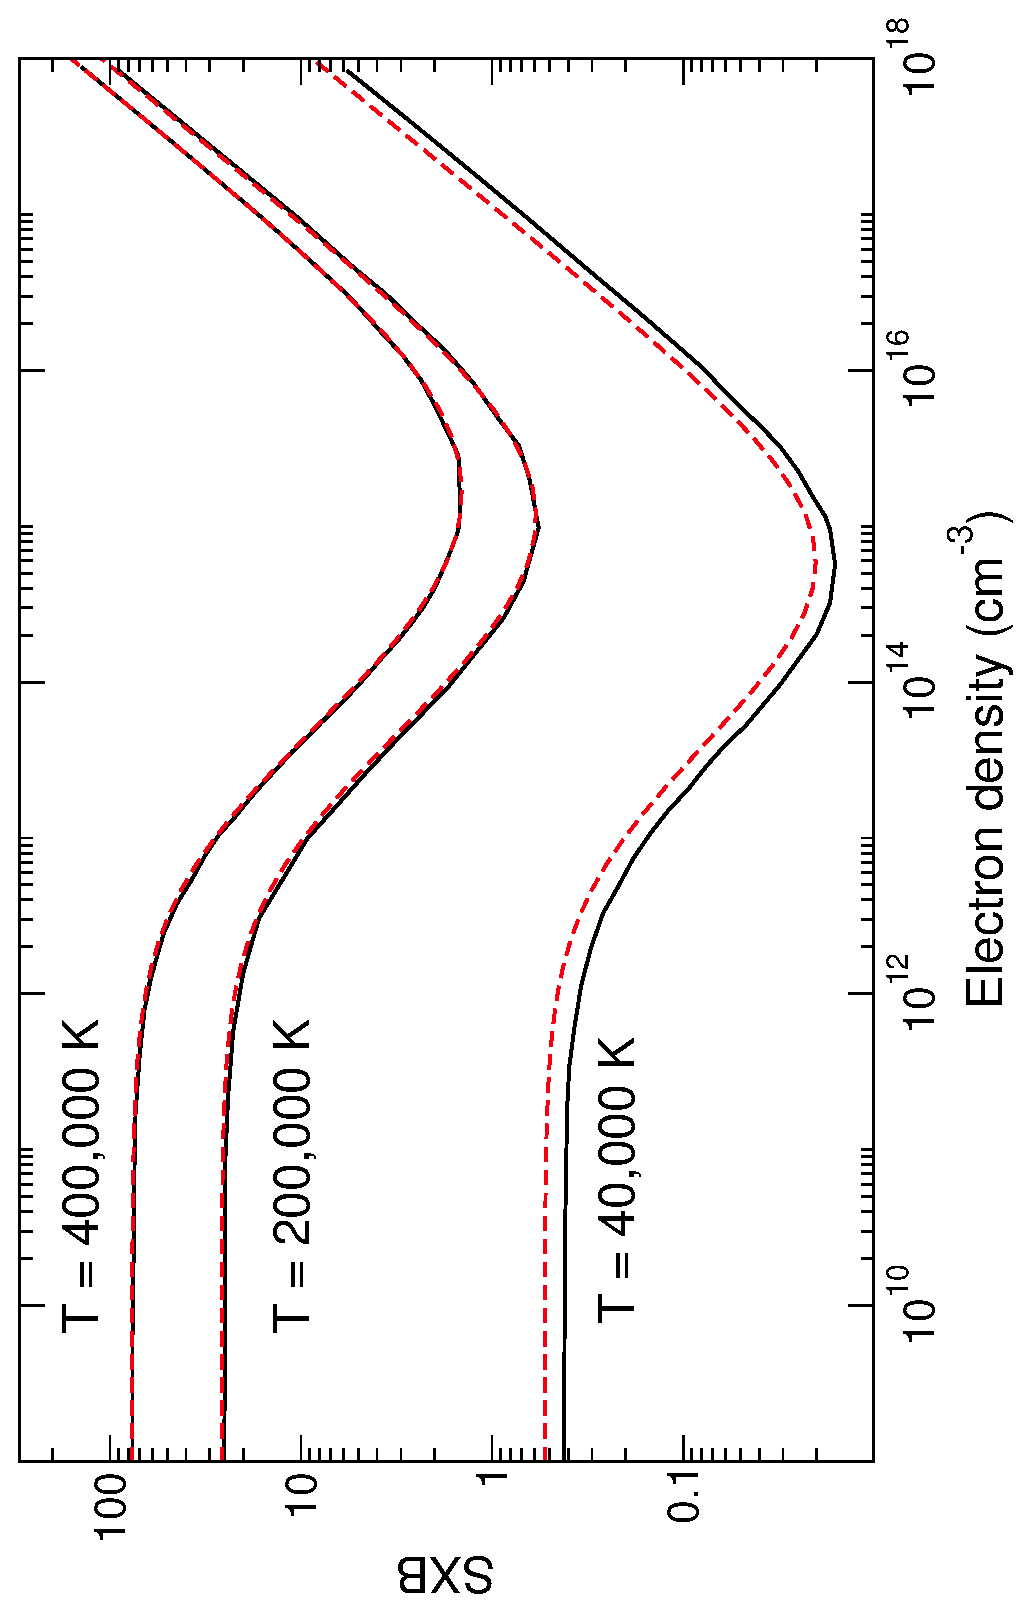
\includegraphics[scale=0.55,angle=-90]{Figures/Spectral/comparison1.eps}
\caption{The $\mathcal{SXB}_{1,3\rightarrow 2}$ ratio for Case 1 as a function of the electron density for three temperatures $T=40,000$ K, $T=200,000$ K, and $T=400,000$ K. The solid black curves are the results from \citet{2007JPhB...40.4537G}, and the dashed red curves are generated with the same input from the {\sc collr-v1.0} computer code. \label{fig:spe_sxb1}}
\end{figure}
%%%%
%%%
%%
%

%
%%
%%%
%%%%
\begin{figure}
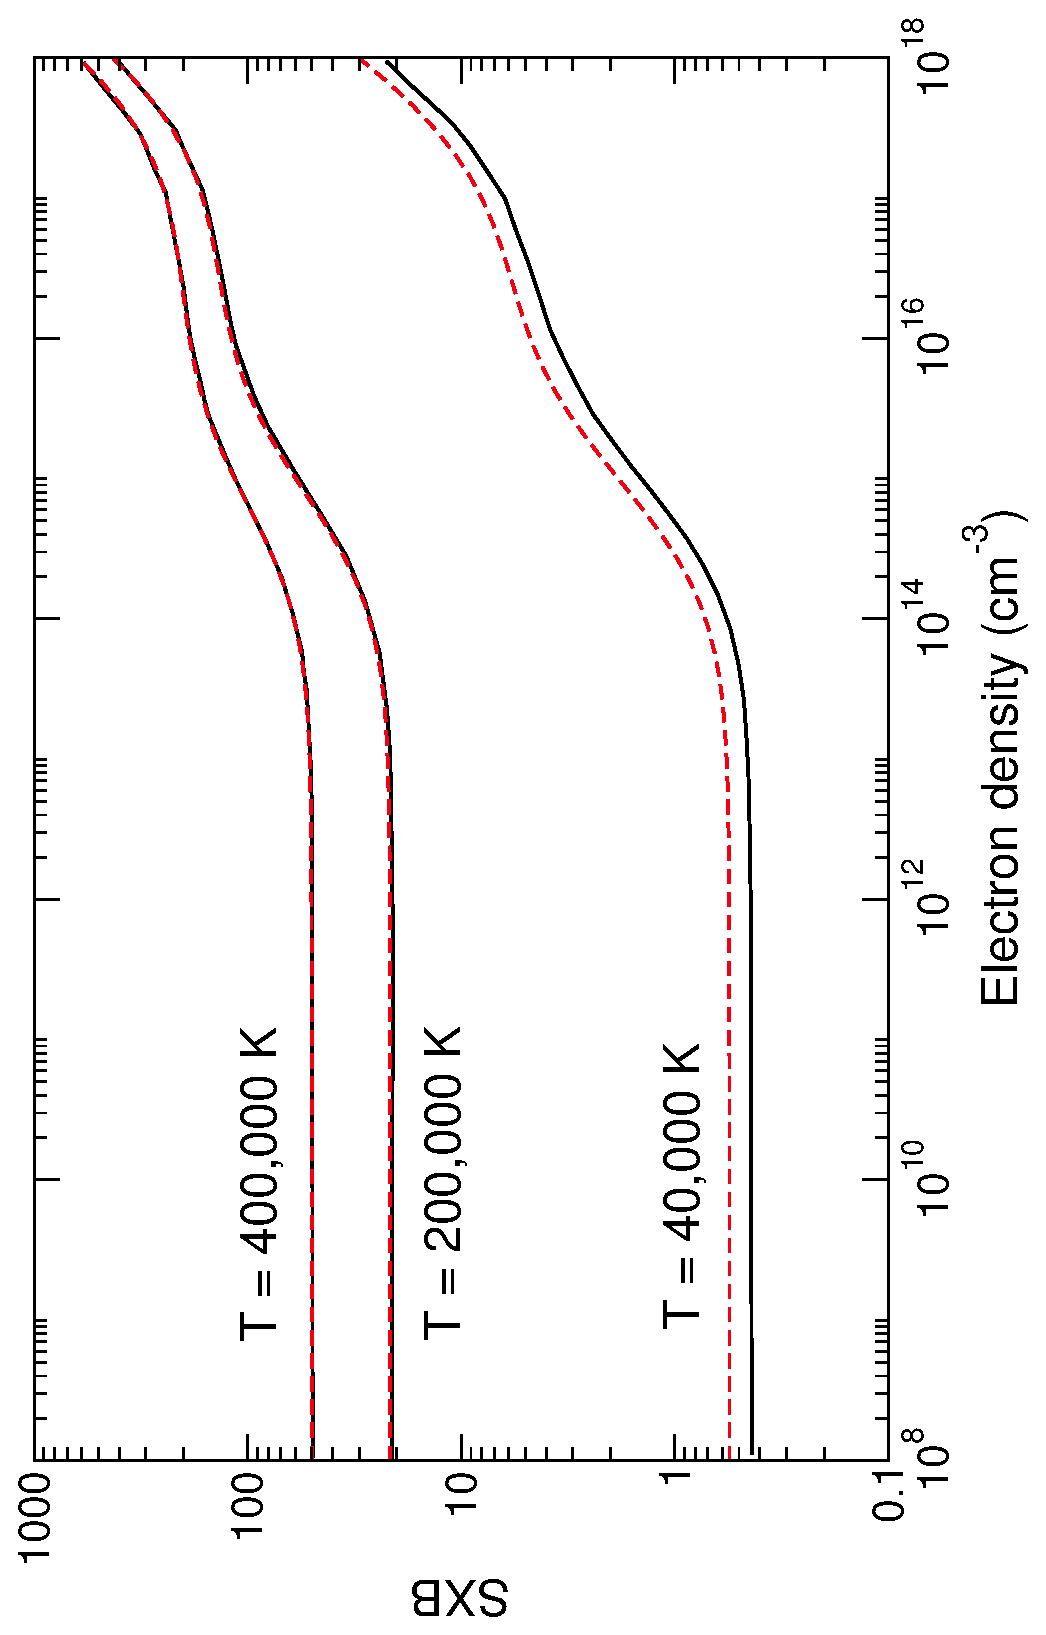
\includegraphics[scale=0.55,angle=-90]{Figures/Spectral/comparison2.eps}
\caption{The $\mathcal{SXB}_{1,3\rightarrow 2}$ ratio for Case 2 as a function of the electron density for three temperatures $T=40,000$ K, $T=200,000$ K, and $T=400,000$ K. The solid black curves are the results from \citet{2007JPhB...40.4537G}, and the dashed red curves are generated with the same input from the {\sc collr-v1.0} computer code. \label{fig:spe_sxb2}}
\end{figure}
%%%%
%%%
%%
%

A useful test is to consider the two limiting cases; LTE (high density), and the coronal approximation (low density), for particular line ratios in equation (\ref{eq:spe_lratio}). Therefore, by applying the two equations (\ref{eq:spe_lte}) and (\ref{eq:spe_coronal}), the values are computed for all temperatures by setting the flags \texttt{corrap=1} and \texttt{lte=1}.

Finally, we can look at particular photon emissivity coefficients over a range of electron temperatures and densities. This is initialized by setting $\texttt{ppec} = 1$, to calculate between an upper ($\texttt{uppec}$), and lower ($\texttt{lopec}$) state. It is also possible to calculate certain line ratios from equation (\ref{eq:spe_lratio}) by setting the following variables,
\[
\mathcal{R} = \frac{I_{\texttt{uplev}\rightarrow \texttt{uplevl}}}{I_{\texttt{lolev} \rightarrow \texttt{lolevl}}} = \frac{N_{\texttt{uplev}} A_{\texttt{uplev}\rightarrow \texttt{uplevl}}}{N_{\texttt{lolev}} A_{\texttt{lolev}\rightarrow \texttt{lolevl}}}\frac{\lambda_{\texttt{lolevl,lolev}}}{\lambda_{\texttt{uplevl,uplev}}} ~~~~~~~ {\rm if} ~~~ \texttt{line = 1}.
\]
To improve and validate the current set of codes, we look at two, three levels systems from the work carried out by \citet{2007JPhB...40.4537G}:\\\\
Case 1: ~~~level 1 - 3p$^5$ $^2$P ~~~level 2 - 3p$^4$4p $^4$D$^{\rm o}$  ~~~level 3 - 3p$^4$4s $^4$P\\
Case 2: ~~~level 1 - 3p$^5$ $^2$P ~~~level 2 - 3p$^4$4p $^2$D$^{\rm o}$ ~~~level 3 - 3p$^4$4s $^2$P.\\\\
We therefore use the input test case of \textit{rad.inp} for Case 1 and Case 2, and compute the $\mathcal{SXB}_{1,3\rightarrow 2}$ ratio from equation (\ref{eq:spe_sxb}). The results for the corresponding cases are shown in Figures \ref{fig:spe_sxb1} and \ref{fig:spe_sxb2} as a function of the electron density for three temperatures of $T=40,000$ K, $T=200,000$ K, and $T=400,000$ K. There is excellent agreement between the magnitude of results and dominant features between the two calculations, with only slight deviation for the low temperature ratio of $T=40,000$ K.
\newpage

\section{Radiative and dielectronic recombination rate coefficients}\label{sec:spe_rranddr}
These astrophysical plasma, as well as laboratory plasma often require descriptions such as those in Section \ref{sec:spe_imp} for ionization and recombination processes. Numerous investigations have been carried out for these recombination processes in low density regimes \citep{1982ApJS...48...95S, 1985A&AS...60..425A, 1991A&A...251..680P}, but more recently work has been focused towards expanding to study NLTE regimes \citep{2003A&A...406.1151B, 2006ApJ...651L..73B, 2005ApJS..158...80N}.

Another extremely important mechanism to consider is determining the ionization balance with neighbouring ion stages, i.e. extending the isolated atom approximation. Currently, {\sc collr-v1.0} does not have the capability to include ionization and recombination rates during the collisional-radiative process.

The definition for the radiative recombination process is the capture of an electron into some bound state. This is precisely the reverse process defined in equation (\ref{eq:rmat_basicphoto}), so we can write
\begin{equation}\label{eq:rmat_basicre}
\begin{split}
& ~~~~~~~~~~~~~~ \tiny{\circled{1}}\\
& h\nu+ X_i^{q+} \leftarrow X_f^{(q+1)+} +e^-\\
& ~~~\tiny{\circled{2}}\nwarrow ~~~~~~~~~~~~~~~~~\swarrow \tiny{\circled{2}} \\
& ~~~~~~~~~~~~(X_y^{q+})^*
\end{split}
\end{equation}
We refer to the process in 1) as radiative recombination (RR) and 2) as dielectronic recombination (DR). Therefore, the $R$-matrix technique provides an approach for calculating the partial recombination rates for a specific transition through all its autoionization states. We write this partial contribution from an initial electron plus ion system to some final bound state as,
\begin{equation}\label{eq:spe_partialrate}
\tilde{\alpha}^{P}_{f\rightarrow i} = \alpha^{RR}_{f\rightarrow i} + \sum_y\alpha^{DR}_{y\rightarrow i}.
\end{equation}
We do not explicitly calculate the total rate, but it can be obtained by summing over all final bound states defined by equation (\ref{eq:spe_partialrate}),
\[
\alpha^{Tot}_f = \sum_i\tilde{\alpha}^{P}_{f\rightarrow i}.
\]
By assuming detailed balance and LTE from equation (\ref{eq:spe_lte}), it is possible to write the photoionization cross-sections in terms of the recombination cross-sections by appling the Milne relation,
\begin{equation}\label{eq:spe_milne}
\frac{\sigma^{r}_{f\rightarrow i}}{\sigma^p_{i\rightarrow f}}= \frac{g_i}{g_f}\frac{(\alpha E)^2}{4\epsilon}.
\end{equation}
$\alpha$ with no subscripts is the fine-structure constant, $E$ is the photon energy in Rydbergs, and $\epsilon$ is the kinetic energy of the electron in Rydbergs. By describing the distribution of electron velocities as Maxwellian in equation (\ref{eq:spe_max}), it is possible now to compute the formal definition for the rates defined in equation (\ref{eq:spe_partialrate}),
\begin{equation}\label{eq:spe_formalrate}
\tilde{\alpha}^P_{f\rightarrow i} = \int\frac{g_i}{2g_f}(\alpha E)^2f(v)\sigma^p_{i\rightarrow f}d\epsilon.
\end{equation}
%
%%
%%%
%%%%
\begin{figure}
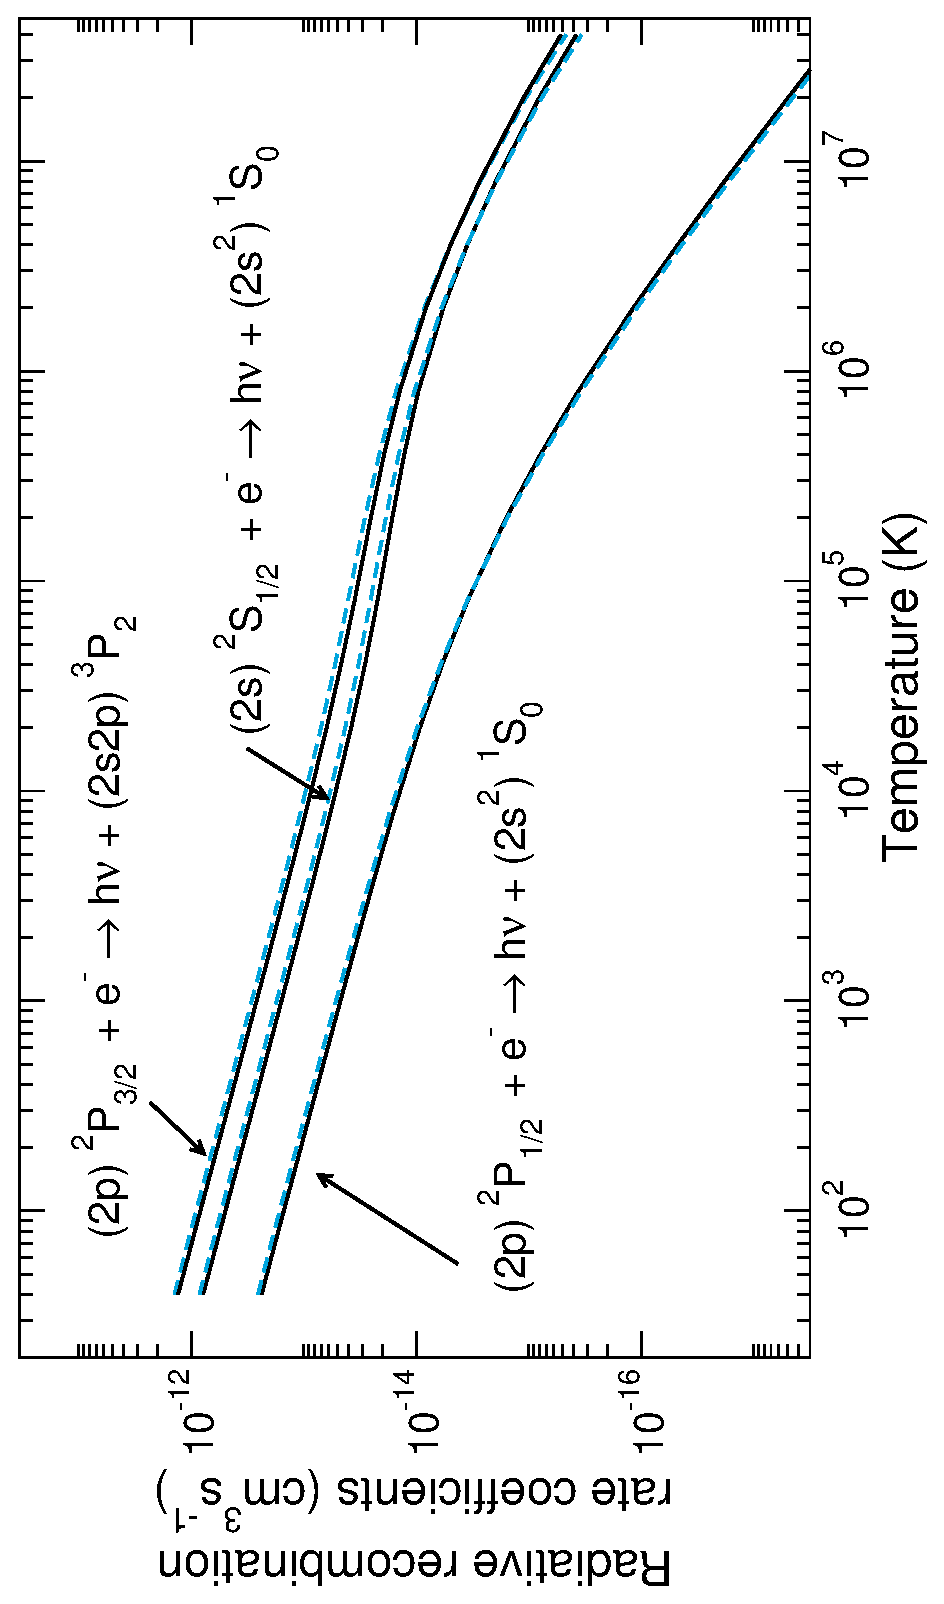
\includegraphics[scale=0.54,angle=-90]{Figures/Spectral/rates/be-like/total.eps}
\caption{Radiative recombination rates in cm$^3$s$^{-1}$ as a function of electron temperature in K. The three transitions plotted are $\tilde{\alpha}^P_{1\rightarrow 1} \equiv$ 2s $^2$S$_{1/2}$ + e$^-$ $\rightarrow$ $h\nu$ + 2s$^2$ $^1$S$_0$, $\tilde{\alpha}^P_{2\rightarrow 1} \equiv$ 2p $^2$P$_{1/2}^{\rm o}$ + e$^-$ $\rightarrow$ $h\nu$ + 2s$^2$ $^1$S$_0$, and $\tilde{\alpha}^P_{3\rightarrow 4} \equiv$ 2p $^2$P$_{3/2}^{\rm o}$ + e$^-$ $\rightarrow$ $h\nu$ + 2s2p $^3$P$_2^{\rm o}$. The black curve are the results from \citet{2006ApJS..167..334B} and the blue dashed curves are the present results.\label{fig:spe_boron}}
\end{figure}
%%%%
%%%
%%
%
where $f(v)$ is the Maxwellian distribution and the integration is over all kinetic energies of the scattered electron. We consider standard integration techniques with data produced using the computer code {\sc autostructure}. The photoionization cross-sections obtained from OPEN-ADAS are transformed to recombination cross-sections by equation (\ref{eq:spe_milne}), which are then used to determine the recombination rates from equation (\ref{eq:spe_formalrate}). We present in Figure \ref{fig:spe_boron} three transitions of Be-like Boron for,\\
$\tilde{\alpha}^P_{1\rightarrow 1} \equiv$ 2s $^2$S$_{1/2}$ + e$^-$ $\rightarrow$ $h\nu$ + 2s$^2$ $^1$S$_0$, \\
$\tilde{\alpha}^P_{2\rightarrow 1} \equiv$ 2p $^2$P$_{1/2}^{\rm o}$ + e$^-$ $\rightarrow$ $h\nu$ + 2s$^2$ $^1$S$_0$,\\
$\tilde{\alpha}^P_{3\rightarrow 4} \equiv$ 2p $^2$P$_{3/2}^{\rm o}$ + e$^-$ $\rightarrow$ $h\nu$ + 2s2p $^3$P$_2^{\rm o}$,\\\\
and compare the blue dashed curves from equation (\ref{eq:spe_formalrate}) with the published rates of \citet{2006ApJS..167..334B} with excellent agreement.

It is therefore possible to compute the partial recombination rates defined by equation (\ref{eq:spe_formalrate}) directly from the photoionization cross-sections that we calculate in equation (\ref{eq:rmat_totphoto}).





%----------------------------------------------------------------------------------------


 
% Chapter 1
%----------------------------------------------------------------------------------------------------------
\chapter{Single photoionization and resonance identification of S$^{8+}$}
% Main chapter title
\label{cha:sulphur} 
% For referencing the chapter elsewhere, use \ref{Chapter1} 
\lhead{Chapter 5. \emph{Photoionization of} S$^{8+}$} 
% This is for the header on each page - perhaps a shortened title
%----------------------------------------------------------------------------------------------------------

                           %                                              %
                          %%%                                    %%%
       %%%%%%%%%%      SECTION     %%%%%%%%%%
                          %%%                                    %%%
                           %                                             %
                           
\section{Introduction}\label{sec:sul_intro}
Now that we have discussed appropriate methods for generating accurate wavefunctions to describe the atomic target, we can avail of them to look at specific systems. Our aim is to implement these wavefunctions into the $R$-matrix method, as described in Chapter \ref{cha:rmatrix}, to compute atomic transitions that are required in a range of astrophysical and plasma applications.

The ions under investigation in this Chapter, S$^{8+}$ (S {\sc ix}) and S$^{9+}$ (S {\sc x}), have received much interest in recent years due to their astrophysical importance, and crucial scientific development has laid the foundations for line emission identifications of S {\sc x}. Examples of such identifications include early observations \cite{1965AnAp...28..755T}, laser produced plasmas in theta pinch experiments \cite{1973PhyS....8..244F, 1987PhyS...36...80F, 1966ApJ...144..435D, 1967ApJ...149..451D}, and more recently, beam-foil techniques \cite{1999PhyS...59..355K}. These important lines are visible in both the UV and soft X-Ray regimes of the electromagnetic spectrum, the latter exclusively arising from transitions of electrons occupying the $n = 3$ shells and in particular, transitions involving the ground state 2s$^2$2p$^3$ ($^4$S$_{3/2}^{\rm o}$). Additional S {\sc x} lines have also been observed spectroscopically in the nearby F-type star Procyon \cite{0004-637X-762-1-53} by instruments on board the Chandra satellite \cite{2000SpiE.4012...81B} as well as in the solar corona above an active region and within the quiet sun \cite{2003ApJ...582.1162M, 2012A&A...537A..38D}, through instruments on board Hinode EIS \cite{2007SoPh..243...19C} and also SOHO \cite{1995SoPh..162....1D}. Such observations are investigated with great scrutiny by modern laboratory techniques using the electron beam ion trap resulting in excellent agreement \cite{2014ApJ...788...25B, 2014ApJS..215....6T}.

For the S$^{9+}$ system there have been a number of publications pertaining to the generation of electron-impact excitation data. Initially \citet{2000ADNDT..76..176B} included only those target levels within the $n = 2$ complex plus one additional configuration, 2s$^{2}$2p$^{2}$3s. Then in 2003, \citet{2003ADNDT..85..169B} extended this work to include all $n = 3$ levels resulting in 34 $LS\pi$ coupled target states using the distorted wave approximation. The most sophisticated work to date was published in 2011 by \citet{2011A&A...533A..87L} who included configurations encompassing 84 levels within the $n = 3$ complex and implementing the intermediate-coupling frame transformation ({\sc icft}) $R$-matrix method. While we are not directly concerned with the electron scattering process, it is clear that the inclusion of all $n = 3$ orbitals and associated target levels is of major importance within our calculation. A consequence of this allows us to incorporate additional correlation when describing all scattering wavefunctions. Despite the lack of photoionization cross-sections within an intermediate coupling scheme available via the Opacity Project, calculations have been carried out elsewhere by Badnell et al. \cite{2005MNRAS.360..458B}. The data is available for download from the OPEN-ADAS compilation, thus providing comparable results. However, only resonance-free partial contributions to each target state are available, so the comparison is limited to background cross-Section only. A much more sophisticated evaluation of level resolved photoionization cross-sections is therefore required in order to benchmark results for appropriate plasma physics diagnostics in non-local thermodynamic equilibrium (NLTE) approximation calculations.

We express the photoionization process for the lowest five initial states of the S$^{8+}$ ion as,
\begin{eqnarray}\label{eq:sul_process}
& h\nu + \text{S}^{8+}~  [2s^22p^4]_{\rm J}  \longrightarrow ~ \text{S}^{9+}~ [2s^x2p^{3+y}3l^z + e^-] \nonumber \\ 
&  \searrow ~~~~ \nearrow\\ \nonumber
& (\text{S}^{8+})^*~ [2s^22p^3nd, 2s2p^4np, nf]
\end{eqnarray} 
where the electron is ejected through one of its channels provided it is open. The process can occur directly (along the top arrow) to leave the target and electron complex, or via a more indirect route which excites the S$^{8+}$ ion to some resonant state before the ejection of a photoelectron into the continuum. These autoionizing states are discussed and identified later in Section \ref{sec:sul_results} of this Chapter using appropriate techniques. This process is calculated for transitions of the nature $J=2, 1$ and $\Delta J = 0, \pm 1$ with the exception of $\Delta J  = 1$ for $J = 0$, allowing for change in parity to be conserved between initial and final states and the selection rules to be adhered, described in Section \ref{sec:many_selection}. The target  S$^{9+}$ can be simplified to the following constraints; $x+y+z = 2$ and $z\leq 1$ for $l = s, p, d$, which will be discussed in greater detail within Section \ref{sec:sul_target}.

\begin{table}[hbt]
\footnotesize
\begin{center}
\begin{tabular}{@{}        l r c r     |      l r c r        @{}}
\toprule
\multicolumn{1}{c}{$nl$} & \multicolumn{1}{c}{$c_{jnl}$} & \multicolumn{1}{c}{$I_{jnl}$} & \multicolumn{1}{c}{$\zeta_{jn}$} & \multicolumn{1}{c}{$nl$} & \multicolumn{1}{c}{$c_{jnl}$} & \multicolumn{1}{c}{$I_{jnl}$} & \multicolumn{1}{c}{$\zeta_{jn}$} \\  

\toprule
    %                                        &                   &     &                    &       &                   &    & \\
    \multicolumn{1}{c}{1s} & 0.95941    & 1 & 15.63090   & 3s  & 0.21735   & 1 & 12.05049\\     
                                            & 0.02266    & 1 & 26.59100   &       & --1.05970 & 2 & 5.00069 \\  
                                            & 0.00360    & 2 & 7.05116     &       & 1.53459   & 3 & 3.73297 \\                                                                    
                                            & 0.02453    & 2 & 13.23750   &       &                  &     & \\
                                            & --0.00197  & 2 & 6.05344     & 2p & 0.48450   & 2 & 6.67108\\
                                            &                    &    &                    &       & 0.08978   & 2 & 10.59010  \\
    \multicolumn{1}{c}{2s} & --0.29633  & 1 & 15.63090  &       & 0.44221   & 2 & 5.62582\\  
                                            & --0.00138  & 1 & 26.59100  &       & 0.00279   & 2 & 20.93410\\                                                                                                                                   
                                            & 0.19810    & 2 & 7.05116    &       &                  &     & \\   
                                            & --0.16315  & 2 & 13.23750  & 3p  & 0.59734   & 2 & 6.35642\\ 
                                            & 0.95388    & 2 & 6.05344    &         & --1.16636 & 3 & 3.47094 \\ 
                                            &                    &    &                   &       &                  &     & \\       
                                            &                    &    &                   &  3d  & 1.00000   & 3 & 3.54124\\
 %                                          &                   &     &                    &       &                   &    & \\      

\bottomrule
 \end{tabular}
  \caption{Orbital parameters for the optimized $n = 3$ orbitals of the radial form (\ref{eq:many_boundorbs}) generated using the computer package \protect{\sc{civ3}}. These orbitals are included alongside the existing Hartree-Fock orbitals of \citet{1974ADNDT..14..177C}. \label{tab:sul_orbitals}}
 \end{center}
\end{table}

%%%%%%%%%% TABLE %%%%%%%%%%%%%

\begin{table}[hbt]
\footnotesize
\begin{center}
\begin{tabular}{@{} l *4c c *3c @{}}
\toprule

\multicolumn{1}{c}{Index} & \multicolumn{1}{c}{Config.} & \multicolumn{1}{c}{Spec.} & \multicolumn{1}{c}{\textit{Martin}} & \multicolumn{1}{c}{\textit{Present}} &  \multicolumn{1}{c}{$\%$ Change} & \multicolumn{1}{c}{\textit{Liang}} & \multicolumn{1}{c}{\textit{Bhatia}} &  \multicolumn{1}{c}{\textit{Fischer}}    \\

\toprule

       \multicolumn{1}{c}{1} & 2s$^22$p$^3$ & $^4$S$^{\rm o}_{3/2}$ & 0.0000 & 0.0000 & 0.00 & 0.0000 & 0.0000 & 0.0000\\
       \multicolumn{1}{c}{2} & -- & $^2$D$^{\rm o}_{3/2}$ & 0.7513 & 0.7813 & 3.84 & 0.7929 & 0.7963 & 0.7568\\
       \multicolumn{1}{c}{3} & -- & $^2$D$^{\rm o}_{5/2}$ & 0.7618 & 0.7973 & 4.45 & 0.8101 & 0.8079 & 0.7681\\
       \multicolumn{1}{c}{4} & -- & $^2$P$^{\rm o}_{1/2}$ & 1.1571 & 1.1628 & 0.49 & 1.1932 & 1.1944 & 1.1597\\
       \multicolumn{1}{c}{5} & -- & $^2$P$^{\rm o}_{3/2}$ & 1.1738 & 1.1812 & 0.63 & 1.2131 & 1.2119 & 1.1765\\
       \multicolumn{1}{c}{6} & 2s2p$^4$ & $^4$P$_{5/2}$ & 3.4488 & 3.4403 & --0.25 & 3.4966 & 3.4954 & 3.4608\\
       \multicolumn{1}{c}{7} & -- & $^4$P$_{3/2}$ & 3.5117 & 3.4995 & --0.35 & 3.5593 & 3.5608 & 3.5239\\
       \multicolumn{1}{c}{8} & -- & $^4$P$_{1/2}$ & 3.5438 & 3.5317 & --0.34 & 3.5933 & 3.5942 & 3.5557\\
       \multicolumn{1}{c}{9} & -- & $^2$D$_{3/2}$ & 4.7452 & 4.8149 & 1.45 & 4.8730 & 4.8739 & 4.7647\\
       \multicolumn{1}{c}{10} & -- & $^2$D$_{5/2}$ & 4.7465 & 4.8185 & 1.49 & 4.8771 & 4.8763 & 4.7660\\
       \multicolumn{1}{c}{11} & -- & $^2$S$_{1/2}$ & 5.5477 & 5.6076 & 1.07 & 5.6861 & 5.6864 & 5.5645\\
       \multicolumn{1}{c}{12} & -- & $^2$P$_{3/2}$ & 5.8038 & 5.9266 & 2.07 & 5.9722 & 5.9715 & 5.8300\\
       \multicolumn{1}{c}{13} & -- & $^2$P$_{1/2}$ & 5.8837 & 6.0032 & 1.99 & 6.0544 & 6.0545 & 5.9101\\
       \multicolumn{1}{c}{14} & 2p$^5$ & $^2$P$^{\rm o}_{3/2}$ & 9.0329 & 9.1913 & 1.72 & 9.2852 & 9.2860 & 9.0635\\
       \multicolumn{1}{c}{15} & -- & $^2$P$^{\rm o}_{1/2}$ & 9.1343 & 9.2933 & 1.71 & 9.3900 & 9.3914 & 9.1650\\                                                                                           
       \multicolumn{1}{c}{16} & 2s$^2$2p$^23$s & $^4$P$_{1/2}$ & 19.0223 & 19.0677 & 0.24 & 18.9961 & 18.9959 & 19.0238\\
       \multicolumn{1}{c}{17} & -- & $^4$P$_{3/2}$ & 19.0674 & 19.1073 & 0.21 & 19.0380 & 19.0379 & 19.0660\\
       \multicolumn{1}{c}{18} & -- & $^4$P$_{5/2}$ & 19.1224 & 19.1648 & 0.22 & 19.0981 & 19.0979 & 19.1226\\       
       \multicolumn{1}{c}{19} & -- & $^2$P$_{1/2}$ & 19.2560 & 19.3011 & 0.23 & 19.2446 & 19.2445 & 19.2535\\       
       \multicolumn{1}{c}{20} & -- & $^2$P$_{3/2}$ & 19.3234 & 19.3698 & 0.24 & 19.3163 & 19.3161 & 19.3221\\       
       \multicolumn{1}{c}{21} & -- & $^2$D$_{5/2}$ & 19.6846 & 19.7480 & 0.32 & 19.6882 & 19.6881 & 19.6950\\
        \multicolumn{1}{c}{22} & -- & $^2$D$_{3/2}$ & 19.6768 & 19.7501 & 0.37 & 19.6907 & 19.6905 & 19.6924\\
        \multicolumn{1}{c}{23} & 2s$^2$2p$^2$3p & $^2$S$_{1/2}$ & -- & 19.9383 & -- & 19.8772 & 19.8771 & 19.8971\\ 
        \multicolumn{1}{c}{24} & -- & $^4$D$_{1/2}$ & -- & 20.0208 & -- & 19.9500 & 19.9499 & 19.9770\\
        \multicolumn{1}{c}{25} & -- & $^4$D$_{3/2}$ & -- & 20.0423 & -- & 19.9719 & 19.9718 & 19.9993\\
        \multicolumn{1}{c}{26} & -- & $^4$D$_{5/2}$ & -- & 20.0805 & -- & 20.0119 & 20.0118 & 20.0389\\
        \multicolumn{1}{c}{27} & -- & $^4$P$_{1/2}$ & -- & 20.1368 & -- & 20.0652 & 20.0651 & 20.0927\\
        \multicolumn{1}{c}{28} & -- & $^4$D$_{7/2}$ & -- & 20.1320 & -- & 20.0659 & 20.0741 & 20.0902\\
        \multicolumn{1}{c}{29} & -- & $^4$P$_{3/2}$ & -- & 20.1465 & -- & 20.0742 & 20.1103 & 20.1002\\
        \multicolumn{1}{c}{30} & -- & $^4$P$_{5/2}$ & -- & 20.1804 & -- & 20.1104 & 20.2001 & 20.1344\\        
\bottomrule
 \end{tabular}
 \caption{Target state energies (in eV) for the lowest 30 fine-structure levels of the target ion S$^{9+}$ relative to the $^4$S$^{\rm o}_{3/2}$ ground state. The column header \textit{Present} represents our current {\sc bprm} calculation, \textit{Martin} are the observed values currently available in the NIST database \citep{1990JPCRD..19..821M}, \textit{Liang} are the electron-impact excitation energies from \cite{0004-637X-762-1-53}, \textit{Bhatia} are those from \cite{2003ADNDT..85..169B} and \textit{Fischer} the structure calculation of \cite{2004ADNDT..87....1F}. The $\%$ change between our \textit{Present} results and \textit{Martin} has also been listed between each level. \label{tab:sul_energy}}
 \end{center}
\end{table}



\begin{table}[t]
\footnotesize
\begin{center}
\begin{tabular}{@{} l *2c @{}}
\toprule

\multicolumn{1}{c}{Main} & \multicolumn{1}{c}{Additional}  \\
\multicolumn{1}{c}{CSFs} & \multicolumn{1}{c}{Correlation CSFs}  \\

\toprule
   %    \multicolumn{1}{c}{} &  \\
       \multicolumn{1}{c}{2s$^2$2p$^3$} & 2p$^4$ [3s, 3p, 3d] \\
        \multicolumn{1}{c}{2s2p$^4$} & 2s2p$^2$ [3s$^2$, 3p$^2$, 3d$^2$] \\
       \multicolumn{1}{c}{2p$^5$} & 2s2p$^2$ [3s3p, 3s3d, 3p3d] \\
          \multicolumn{1}{c}{2s$^2$2p$^2$ [3s, 3p, 3d]}   & 2s$^2$2p [3s$^2$, 3p$^2$, 3d$^2$] \\
           \multicolumn{1}{c}{2s2p$^3$ [3s, 3p, 3d]} & 2s$^2$2p [3s3p, 3s3d, 3p3d] \\
                    & 2p$^3$ [3s$^2$, 3p$^2$, 3d$^2$] \\
                    & 2p$^3$ [3s3p, 3p3d, 3s3d] \\
      %          \multicolumn{1}{c}{} &  \\           
\bottomrule
 \end{tabular}
 \caption{Presented is a list of configurations included in the structure calculation, where square brackets define the assignment of the outermost orbitals pertaining to a common core of 1s$^2$. Provided are 9 main CSF's describing the 215 J$\pi$ levels and 21 additional CSF's for the inclusion of extra correlation. \label{tab:sul_ci}}
 \end{center}
\end{table}

\begin{table}[t]
\footnotesize
\begin{center}
\begin{tabular}{@{} l *6c @{}}
\toprule
\multicolumn{1}{c}{} & \multicolumn{1}{c}{NIST} & \multicolumn{1}{c}{Gu} & \multicolumn{1}{c}{Zheng} & \multicolumn{1}{c}{{\sc mcdf}} & \multicolumn{1}{c}{{\sc top}base} & \multicolumn{1}{c}{\textit{Present}} \\
 \toprule
     %   \multicolumn{1}{c}{} &  & &  &  &  &  \\
       \multicolumn{1}{c}{IP}& 379.84 & 379.63 & 379.10 & 377.78 & 378.67& 381.09 \\
        \multicolumn{1}{c}{$\Delta$IP} & 0.00 & --0.22 & --0.75 & --2.07 & --1.17 & 1.25\\
  %      \multicolumn{1}{c}{} &  & &  &  &  &  \\  
\bottomrule
 \end{tabular}
 \caption{A comparison of the ionization potential (IP) of S$^{8+}$ for a variety of theoretical calculations and our \textit{Present} result, where IP given in eV. $\Delta$IP represents the change in the ionization potential between NIST and the theoretical results. \label{tab:sul_ip}}
 \end{center}
\end{table}

                           %                                              %
                          %%%                                    %%%
       %%%%%%%%%%      SECTION     %%%%%%%%%%
                          %%%                                    %%%
                           %                                             %
\section{Target model}\label{sec:sul_target}
The first step of the $R$-matrix calculation consists of defining a set of basis functions to describe the system after photoionization occurs, in this case, S$^{9+}$ with atomic number $Z=16$ and $N=7$ electrons. The wavefunctions we choose for this system are configuration-interaction expansions of Configuration State Functions (CSF's) built with an orthogonal orbital basis set, taking the form of equation (\ref{eq:many_boundorbs}), with optimized coefficients $c_{jnl}, I_{jnl}$ and $\zeta_{jnl}$ determined by minimizing the total energy of different atomic states. We therefore consider the theory as outlined in Subsection \ref{sec:many_ci} for obtaining configuration-interaction wavefunctions.

The $1s$, $2s$ and $2p$ orbitals are Hartree-Fock orbitals from \citet{1974ADNDT..14..177C} and the $n=3$ orbitals have been optimized using the computer package {\sc civ3} \cite{1975CoPhC...9..141H}, described in Section \ref{sec:many_civ3}. Optimization of the orbital parameters is performed in $LS$ coupling, however, the wavefunctions used to determine the calculated S$^{9+}$ energies are obtained by adding the operators of the {\sc bp} Hamiltonian from equations (\ref{eq:many_bp1}), (\ref{eq:many_bp2}) and (\ref{eq:many_bp3}), to the non-relativistic Hamiltonian. The optimization was then carried out by minimizing on the lowest lying energy levels of the 2p$^2$3$l$ quartet and doublet states ($^4$P for $l=0$, $^4$P$^{\rm o}$ for $l=1$ and $^2$P for $l=2$) respectively. The parameters $c_{jnl}$, $I_{jnl}$ and $\zeta_{jnl}$ adopted for each $n = 3$ orbital are provided in Table \ref{tab:sul_orbitals}.

Table \ref{tab:sul_energy} presents the energies in eV obtained from the current model for the 30 lowest-lying fine-structure levels of the S$^{9+}$ ion relative to the 2s$^{2}$2p$^{3}$ $^{4}$S$^{\rm{o}}_{3/2}$ ground state. The energies were calculated in $LSJ$ coupling and by incorporating all CSF's listed in Table \ref{tab:sul_ci}. We compare with a variety of other theoretical calculations, Liang et al. \cite{2011A&A...533A..87L}, Bhatia and Landi \cite{2003ADNDT..85..169B} and the {\sc mchf} structure approach of \citet{2004ADNDT..87....1F}, and finally the observational values provided by \citet{1990JPCRD..19..821M}. Also listed are the \% differences between our present values and the observed values, highlighting the excellent agreement found for all levels considered. An excellent comparison is also evident between all of the theoretical predictions with the {\sc mchf} values of Fischer closest in agreement to \citet{1990JPCRD..19..821M} as expected, since this evaluation includes all relativistic operators apart from the spin-spin interaction and a large configuration-interaction expansion. For higher lying levels not considered in Table \ref{tab:sul_energy}, a similar accuracy is found. 

Finally in Table \ref{tab:sul_ip}, we summarize the measurements of the S$^{8+}$ ionization potential currently available in the literature, and compare with the value obtained from our current model. Bi\'{e}mont et al. \cite{1999ADNDT..71..117B} performed a fitting to a proposed series expansion of the ionization potential along iso-electronic sequences between previous NIST results and that of Multi-Configuration Dirac-Fock ({\sc mcdf}) calculations, which has been outlined briefly in Subsection \ref{ssec:many_mchf}. NIST has since been updated with this current value. Work carried out by Gu \cite{2005ADNDT..89..267G} involves a Dirac-Coulomb-Breit Hamiltonian for solving the TISE and an extensive configuration-interaction calculation to represent the wavefunctions. Zheng et al. \cite{2002PhRvA..65e2510Z} consider a potential term to describe the weakest bound electron when solving the TISE with a non-relativistic Hamiltonian, and by further extending this to include relativistic corrections. The {\sc mcdf} result has been generated through the computer codes of Grant et al. \cite{1980CoPhC..21..207G}. The TOPbase value is the bound state threshold in $LS$ coupling. The final entry represents our current {\sc bprm} work of 381.10 eV which lies approximately 1.22 eV (or less than 1\%) above the observed NIST value. Overall, excellent agreement is evident between the range of various techniques.

Much deliberation has therefore gone into the preliminary stage of the work in order to limit computational resources needed for the photoionization calculations. After considering many models, we opted for a S$^{9+}$ basis set of 94 $LS\pi$ states which results in 215 $J\pi$ fine-structure levels. We present in Table \ref{tab:sul_ci} the 9 main CSF's that represent the S$^{9+}$ states with an additional 21 configurations of the configuration-interaction expansion accounting for internal, semi-internal and external correlation necessary for improving the wavefunctions. This approach has been described previously in Section \ref{sec:many_config}.

                           %                                              %
                          %%%                                    %%%
       %%%%%%%%%%      SECTION     %%%%%%%%%%
                          %%%                                    %%%
                           %                                             %
                           
\section{Results and discussions}\label{sec:sul_results}
To remain consistent with the wavefunction expansions obtained in the computer package {\sc civ3}, we use the same Hamiltonian operators and therefore employ the {\sc bprm} suite of computer codes described in Section \ref{sec:codes} and Subsection \ref{ssec:BP}. Within the $R$-matrix framework, we select $r=4.6$ Bohr radii allowing convergence of the bound orbitals at the boundary as a consequence of their description in Table \ref{tab:sul_orbitals}. A total of 20 basis functions are chosen to represent the continuum when solving the radial component of the TISE. When constructing the scattering wavefunctions defined by equation (\ref{eq:rmat_boundbasis}), and equation (\ref{eq:rmat_freebasis}), we allow for triple excitation of electrons from the base configuration 1s$^2$2s$^2$2p$^4$ into the remaining $n=3$ complex maintaining a closed 1s$^2$ core. This generates numerous configurations to describe each state of our system and therefore the exploitation of parallel processing is essential in distributing routines through a systematic approach. 


\begin{figure}[hbt]
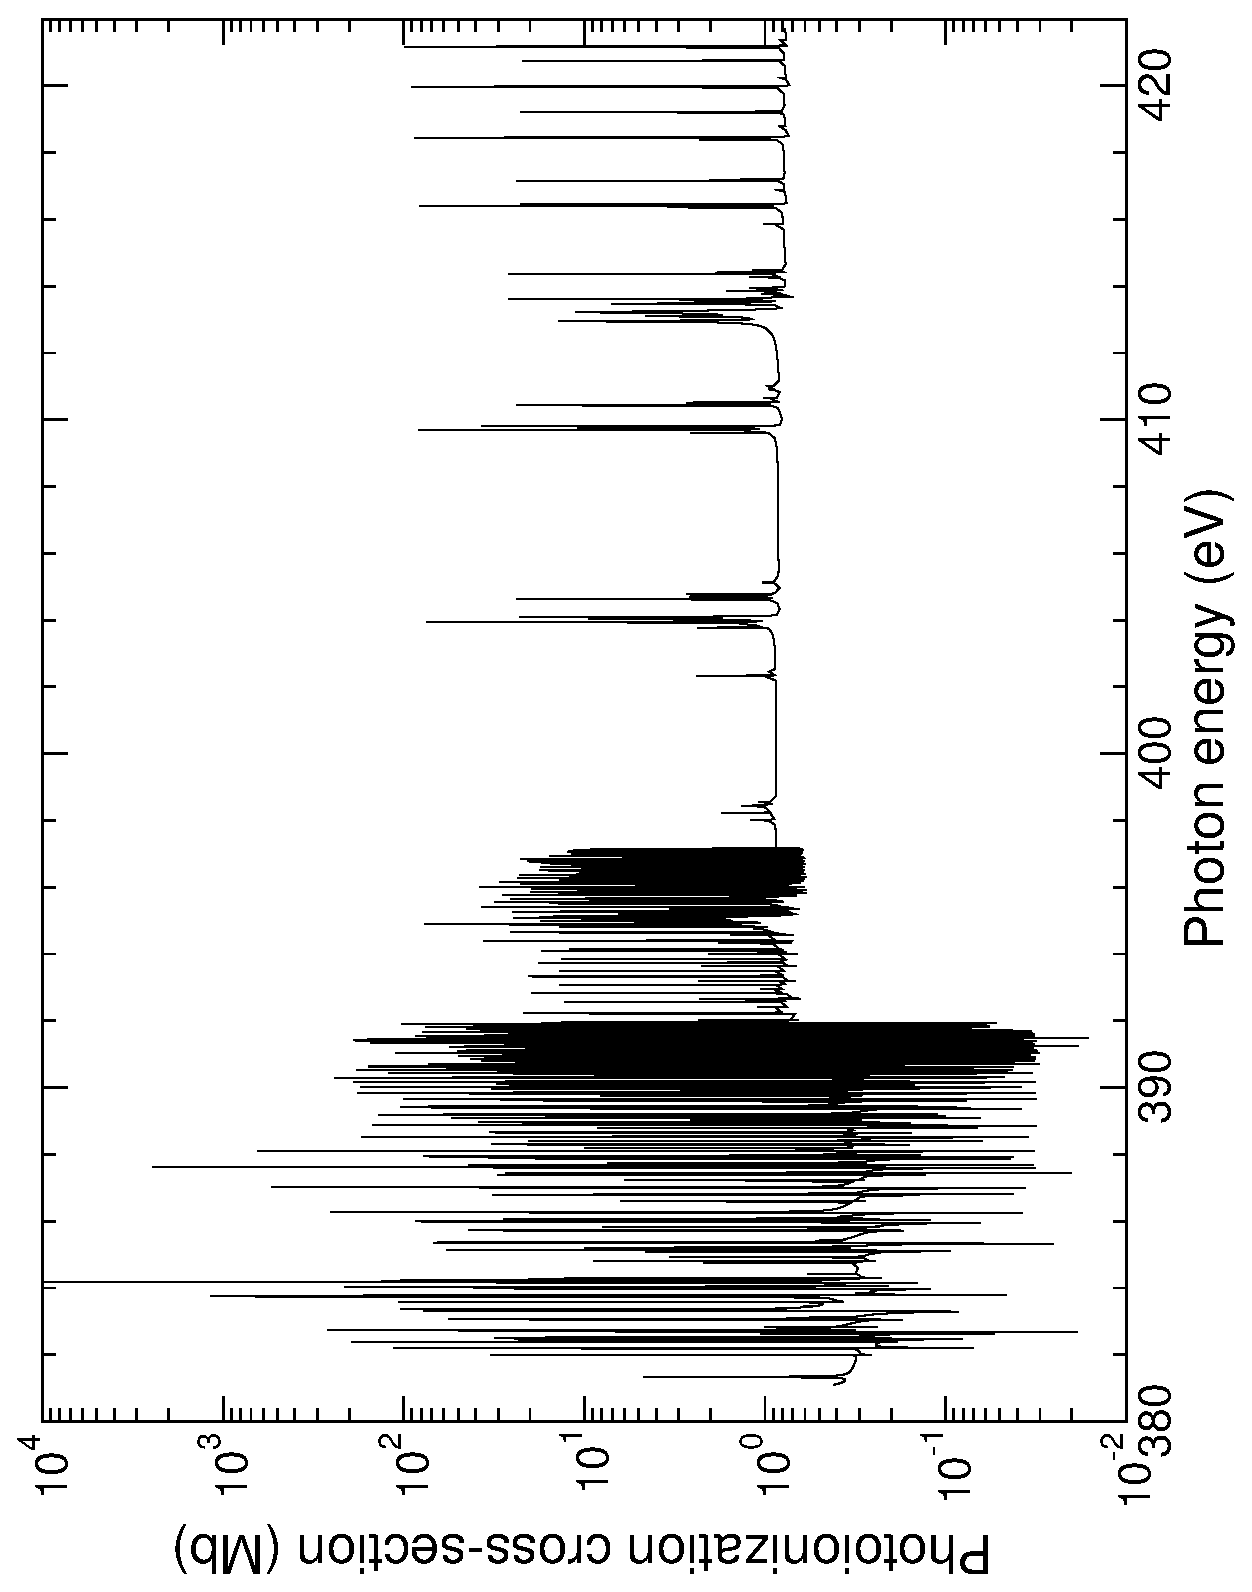
\includegraphics[scale=0.55, angle=-90]{Figures/Sulphur/ground/ground.eps}
\caption{Photoionization cross-section presented on a logarithmic scale in Mb as a function of photon energy in eV, between 380 - 420 eV. We show the fine-structure spectrum of the 2s$^2$2p$^4$ $^3$P$_2$ initial ground state to all allowed $J=1,2,3$ odd final states.\label{fig:sul_ground}}
\end{figure}

After obtaining initial and final state wavefunctions $\Psi_i$ and $\Psi_f$ from equations (\ref{eq:rmat_boundbasis}) and (\ref{eq:rmat_freebasis2}), and also the dipole moment contribution from the internal region defined in equations (\ref{eq:rmat_diplength}) and (\ref{eq:rmat_fullmatrix}), we then calculate the photoionization cross-section $\sigma_{PI}$ as defined in equation (\ref{eq:rmat_totphoto}). For each transition of interest, the photoionization cross-sections are computed for a range of photoelectron energies between 0 - 65 eV. This range for our spectrum is generated via a very fine energy mesh step size of $\approx 6.6 \times 10^{-5}$ eV to ensure that all complex resonance structures have been properly resolved. We also introduce the residual ion charge denoted as $z$ ($=Z-N$). Since length and velocity forms of the dipole approximations discussed in equation (\ref{eq:rmat_diplength}) and (\ref{eq:rmat_diplength}) are in good agreement, length gauge is considered to be the standard throughout. Up to 45 eV the difference in results is within 20\% and therefore all results are provided in the length gauge.

All photoionization scattering cross-sections have been computed within the intermediate coupling scheme, so that the ground and metastable states require dipole matrix transitions of the $J=2$ even state to allowed $J=1,2,3$ odd parity states (ground state $^3$P$_2$), the $J=1$ even state to $J=0,1,2$ odd states (first metastable $^3$P$_1$) and finally the $J=0$ even state to its only accessible final state of $J=1$ odd (second metastable $^3$P$_0$) due to the dipole selection rules.  We also present photoionization cross-sections for the next (lowest) two excited singlet states of the S$^{8+}$ ion, $^1$D$_2$ and $^1$S$_0$ respectively.

%
%%
%%%
%%%%
\begin{sidewaysfigure}
\centering
\includegraphics[scale=0.74, angle=-90]{Figures/Sulphur/meta/meta.eps}
\caption{Photoionization cross-sections presented on a logarithmic scale in Mb as a function of photon energy in eV for the remainder of metastable initial state transitions of the split $^3$P ground state, $^3$P$_1$ (top left) and $^3$P$_0$ (top right). The remaining figures display results for the lowest two excited initial singlet states, $^1$D$_2$ (bottom left) and $^1$S$_0$ (bottom right) to all allowed final states. \label{fig:sul_meta}}
\end{sidewaysfigure}

%
%%
%%%
%%%%
\begin{sidewaysfigure}
\centering
\includegraphics[scale=0.74, angle=-90]{Figures/Sulphur/target/target.eps}
\caption{Partial photoionization cross-sections on a logarithmic scale in Mb as a function of photon energy in eV. The contributions are transitions from the $^3$P$_2$ ground state to the lowest 4 final target levels $^4$S$^{\rm{o}}_{3/2}$ (top left), $^2$D$^{\rm{o}}_{3/2}$ (top right), $^2$D$^{\rm{o}}_{5/2}$ (bottom left), and $^2$P$^{\rm{o}}_{1/2}$ (bottom right) retaining to the 1s$^22$s$^2$2p$^3$ configuration through all allowed channels of the scattering electron. The circles represent results provided by the OPEN-ADAS website. \label{fig:sul_target}}
\end{sidewaysfigure}

We present first in Figure \ref{fig:sul_ground} the photoionization cross-section for the 2s$^2$2p$^4$ $^3$P$_2$ initial state of S$^{8+}$ on a logarithmic scale as a function of the photon energy in eV. All possible allowed final states of the S$^{9+}$ ion have been considered in producing this figure. Clearly visible are the Rydberg resonance series converging onto the target state thresholds. There is currently no direct data in the literature with which we can compare our total photoionization results with.

In Figure \ref{fig:sul_meta} we present similar figures representing photoionization cross-sections for the remaining metastable states $^3$P$_1$ (top left) and $^3$P$_0$ (top right) of the S$^{8+}$ ion, together with results for the first two excited singlet states $^1$D$_2$ (bottom left) and $^1$S$_0$ (bottom right) Again all allowed accessible levels of the final S$^{9+}$ ion are considered and care has been taken to ensure a proper delineation of the Rydberg resonance series converging onto the target state thresholds.

Generally, we require data from metastable and excited levels, as not every S$^{8+}$ ion will be in its ground state when considering specific astrophysical objects. In Section \ref{sec:sul_intro} we referred to a limited set of resonance-free partial photoionization cross-sections available for download from the OPEN-ADAS database \cite{2005MNRAS.360..458B}. In Figure \ref{fig:sul_target} we present partial photoionization cross-sections to the lowest four target level contributions of the S$^{9+}$ ion, $^4$S$^{\rm{o}}_{3/2}$ (top left), $^2$D$^{\rm{o}}_{3/2}$ (top right), $^2$D$^{\rm{o}}_{5/2}$ (bottom left), and $^2$P$^{\rm{o}}_{1/2}$ (bottom right) respectively, which correspond to transitions from the ground $^3$P$_2$ initial state of S$^{8+}$. Excellent agreement is evident for all four partial contributions across this low photoelectron energy range considered. The limited background values from OPEN-ADAS, although neglecting all resonance features, are in line with our base background photoionization cross-sections.

%
%%
%%%
%%%%
\begin{figure}[hbt]
\centering
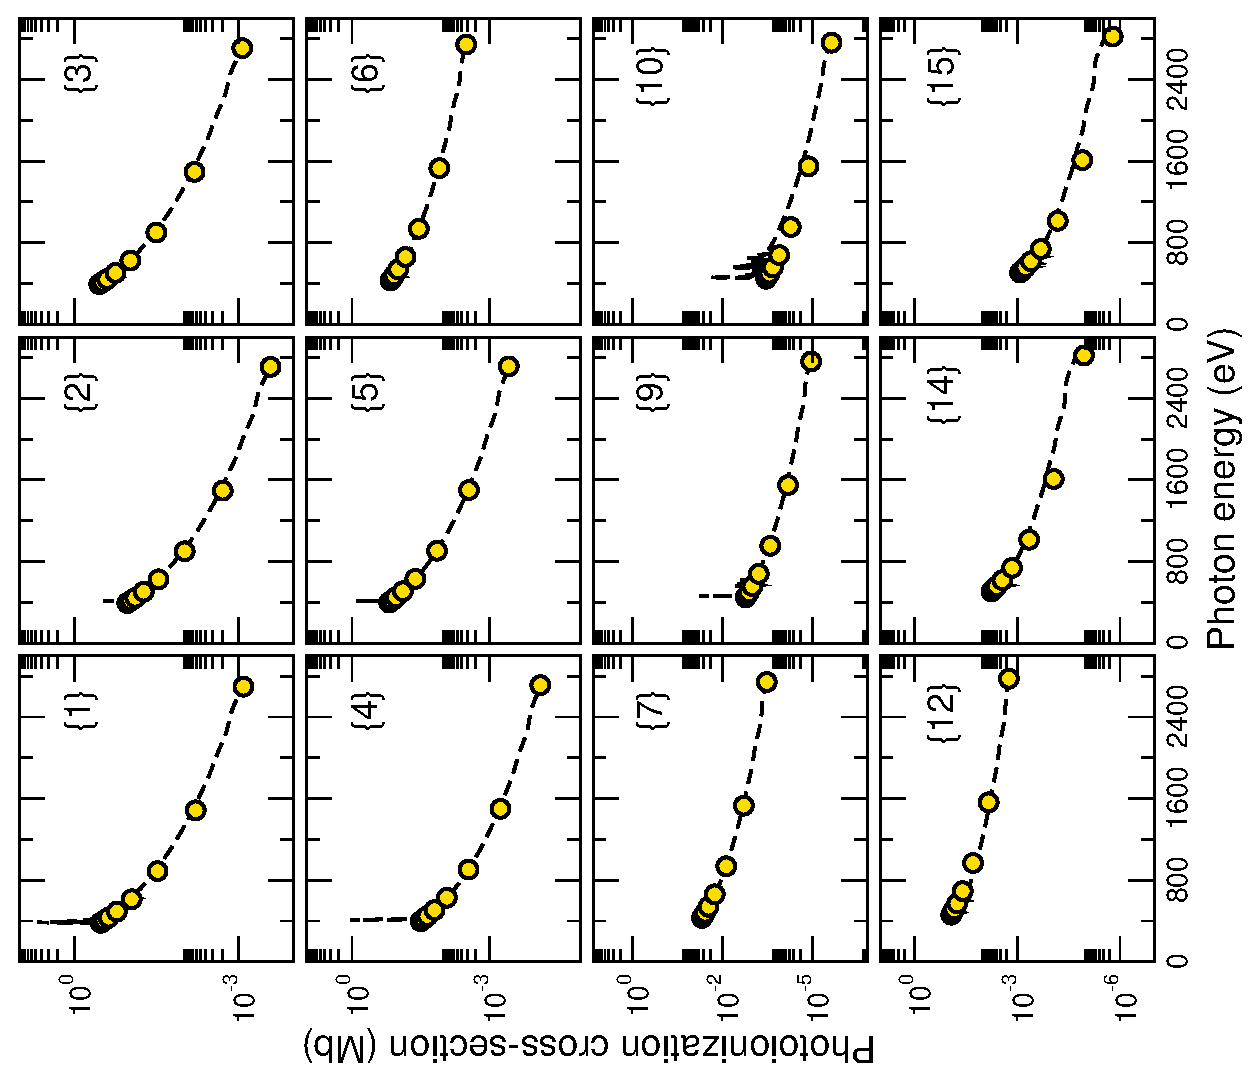
\includegraphics[scale=0.82, angle=-90]{Figures/Sulphur/open-adas/comparison1_new.eps}
\caption{Photoionization cross-sections presented on a logarithmic scale in Mb as a function of photon energy in eV up to 2,700 eV. Transitions are from the initial $^3$P$_2$ $\longrightarrow$ \{1\}, \{2\}, \{3\}, \{4\}, \{5\}, \{6\}, \{7\}, \{9\}, \{10\}, \{12\}, \{14\}, \{15\}. \label{fig:sul_adas2e}}
\end{figure}
%%%%
%%%
%%
%

%
%%
%%%
%%%%
\begin{figure}[hbt]
\centering
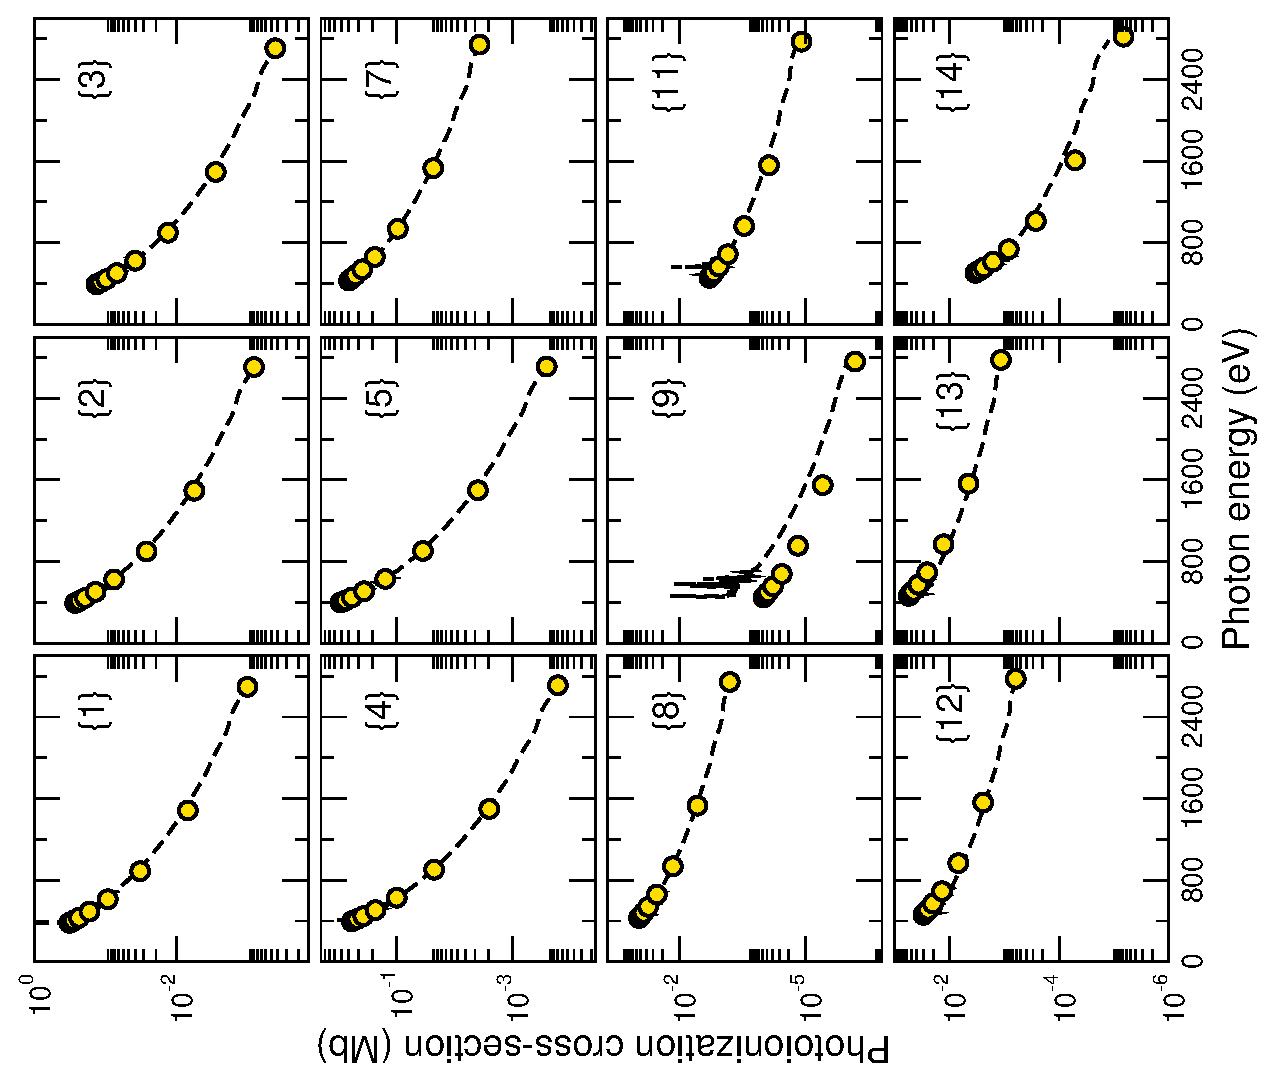
\includegraphics[scale=0.82, angle=-90]{Figures/Sulphur/open-adas/comparison2_new.eps}
\caption{Photoionization cross-sections presented on a logarithmic scale in Mb as a function of photon energy in eV up to 2,700 eV. Transitions are from the initial $^3$P$_1$ $\longrightarrow$ \{1\}, \{2\}, \{3\}, \{4\}, \{5\}, \{7\}, \{8\}, \{9\}, \{11\}, \{12\}, \{13\}, \{14\}. \label{fig:sul_adas1e}}
\end{figure}
%%%%
%%%
%%
%

%
%%
%%%
%%%%
\begin{figure}[hbt]
\centering
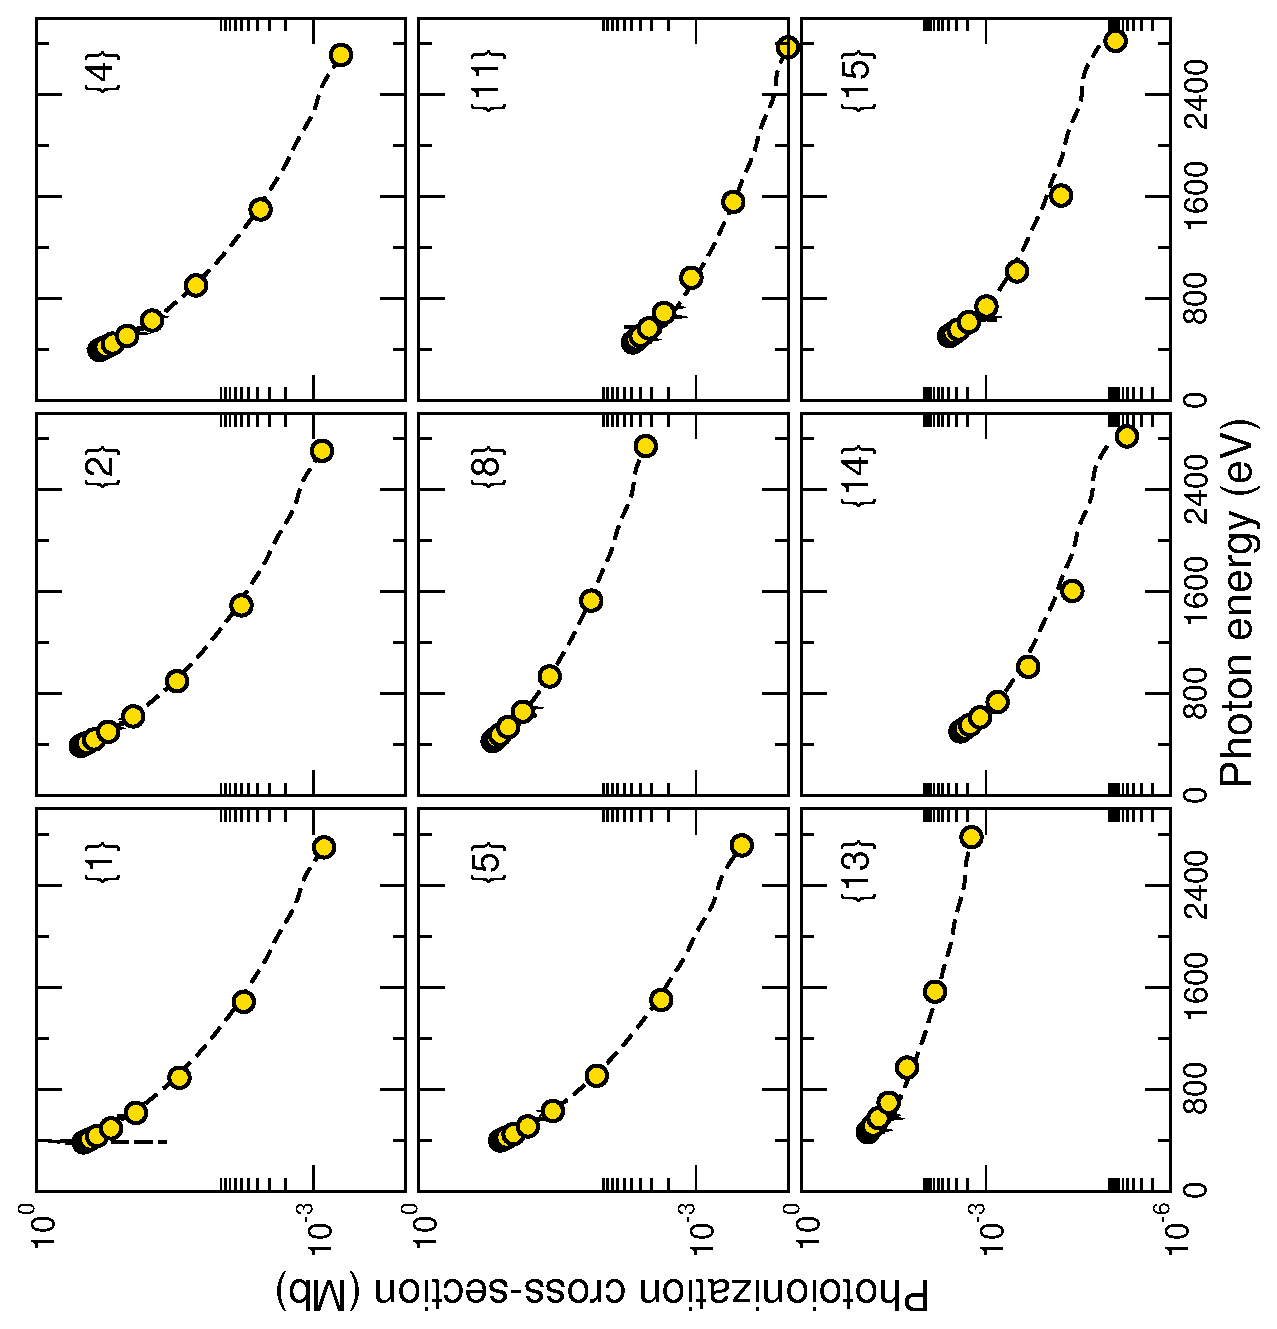
\includegraphics[scale=0.665, angle=-90]{Figures/Sulphur/open-adas/comparison3_new.eps}
\caption{Photoionization cross-sections presented on a logarithmic scale in Mb as a function of photon energy in eV up to 2,700 eV. Transitions are from the initial $^3$P$_0$ $\longrightarrow$ \{1\}, \{2\}, \{4\}, \{5\}, \{8\}, \{11\}, \{13\}, \{14\}, \{15\}. \label{fig:sul_adas0e}}
\end{figure}
%%%%
%%%
%%
%

We also present all possible comparisons with OPEN-ADAS for the lowest initial $^3$P split levels as a further measure of accuracy. A much larger energy mesh is adopted, as we consider just 500 equally spaced energy points across a range of 2,700 eV. This is the maximum energy we can achieve with the basis set employed. Figure \ref{fig:sul_adas2e} shows $^3$P$_2$ and Figures \ref{fig:sul_adas1e} and \ref{fig:sul_adas0e} contain the remaining $^3$P$_1$ and $^3$P$_0$ initial states respectively. We list the transitions within each of the captions, and for brevity, $\{$i$\}$ denotes the corresponding index in Table \ref{tab:sul_energy}. We see that excellent conformity is achieved for nearly all transitions but there are few discrepancies as expected from the two different approaches. The only major differences arise from Figure \ref{fig:sul_adas2e} and Figure \ref{fig:sul_adas1e} where the much weaker transitions are identified as h$\nu$ + $^3$P$_2$ $\rightarrow$ 2s2p$^4$ $^2$D$_{5/2}$ + e$^-$, and h$\nu$ + $^3$P$_1$ $\rightarrow$ 2s2p$^4$ $^2$D$_{3/2}$ + e$^-$ respectively, especially for the low energy region. 


                           %                                              %
                          %%%                                    %%%
       %%%%%%%%%%      SECTION     %%%%%%%%%%
                          %%%                                    %%%
                           %                                             %

\section{Resonance identification}
In this final Section we deal with the identification of the major resonant structure occurring due to autoionizing bound states arising from the indirect pathway scheme (\ref{eq:sul_process}). This identification can be achieved via the $QB$ technique as described in Section \ref{sec:rmat_qb}. We take $E_r$ as the energy position at resonance, $E_{n\rightarrow\infty}$ is the threshold in which each series converges to, and $z=9$. The limiting energy at $E_{n\rightarrow\infty}$ is taken simply as the target threshold value in Table \ref{tab:sul_energy}, which allows us to extract the quantum defects $\mu$ for each $E_r$ computed corresponding to equation (\ref{eq:rmat_qbdefect}). Resonance widths in this method are defined by equation (\ref{eq:rmat_qbwidth}), which incorporates the eigenphase sum and its energy derivative at the resonance position

%
%%
%%%
%%%%
\begin{figure}[hbt]
\includegraphics[scale=0.53, angle=-90]{Figures/Sulphur/threshold_single/threshold_single.eps}
\caption{Various photoionization cross-sections are presented on a logarithmic scale in Mb as a function of photoelectron energy given in eV. The first few resonances occur from the initial $LSJ$ states $^3$P$_2$, $^3$P$_1$, $^3$P$_0$, $^1$D$_2$ and $^1$S$_0$. We present the $J = 1$ odd resonance features and singular $J = 0$ odd resonance. \label{fig:sul_thresh}}
\end{figure}
%%%%
%%%
%%
%

A number of interesting resonance features appear clearly within the photoionization spectra displayed in Figures \ref{fig:sul_ground}, \ref{fig:sul_meta} and \ref{fig:sul_target}. In this Section we have identified the major contributors and estimate their widths in an intermediate coupling frame. There are obvious restrictions and limitations in displaying every resonance that has been identified, therefore only dominant contributions are considered.

%
%%
%%%
%%%%
\begin{sidewaysfigure}
\centering
\includegraphics[scale=0.85, angle=-90]{Figures/Sulphur/resonances/resonance1.eps}
\caption{The total ground state photoionization cross-section is presented on a logarithmic scale as a function of photon energy in eV. Presented are 2 major series that have common parent term $\Lambda_2$ and $\Lambda_3$ coupled to $l=2$ electrons and also the primary members of the $\Lambda_4$, $\Lambda_5$ and $\Lambda_8$ series. These are for select $J =1,2,3$ odd resonances exclusively. \label{fig:sul_resonances1}}
\end{sidewaysfigure}
%%%%
%%%
%%
%

%
%%
%%%
%%%%
\begin{sidewaysfigure}
\centering
\includegraphics[scale=0.85, angle=-90]{Figures/Sulphur/resonances/resonance2.eps}
\caption{The total ground state photoionization cross-section is presented on a logarithmic scale as a function of photon energy in eV. Presented are the resonances with common parent term $\Lambda_4$ and $\Lambda_5$ coupled to $l=2$ electrons and also primary members of the $\Lambda_6$ and $\Lambda_7$ series. These are for select $J =1,2,3$ odd resonances exclusively. \label{fig:sul_resonances2}}
\end{sidewaysfigure}
%%%%
%%%
%%
%

%
%%
%%%
%%%%
\begin{sidewaysfigure}
\centering
\includegraphics[scale=0.85, angle=-90]{Figures/Sulphur/resonances/resonance3.eps}
\caption{The total ground state photoionization cross-section is presented on a logarithmic scale as a function of photon energy in eV. Presented are the resonances with common parent term $\Lambda_6$, $\Lambda_7$ and also those of $\Lambda_8$ coupled to specific $l=1$ and $l=3$ electrons. These are for select $J =1,2,3$ odd resonances exclusively. \label{fig:sul_resonances3}}
\end{sidewaysfigure}
%%%%
%%%
%%
%


In order to convey these identifications visually, we divide the spectrum of Figure \ref{fig:sul_ground}, (depicting the ground state $^3$P$_2$ to the accessible $J=1, 2, 3$ odd states) into appropriate energy ranges. Each series of resonances that converges onto a single threshold we label to be $\Lambda_\zeta$ where the index is given in the first column of Table \ref{tab:sul_energy} and $\Lambda$ denoted as the parent term allocated to each $\zeta$. In our case, we consider those resonances up to and including convergence to the 8th threshold energy, $\Lambda_8 \equiv$ 2s2p$^4$ $^4$P$_{1/2}$.

Before beginning an extensive calculation, we are only required to analyse the ground state transition when considering the dominant $J=1, 2, 3$ odd state resonances. From Figure \ref{fig:sul_thresh}, all initial states of Figure \ref{fig:sul_ground} and Figure \ref{fig:sul_meta} are plotted as a function of photoelectron energy in eV. As expected, the $J = 1$ odd resonance ($\Gamma = 8.83$ meV) at $\approx 0.245$ eV is accessible through the initial states of $^3$P$_2$, $^3$P$_0$, $^1$S$_0$ and $^1$D$_2$. The much narrower $J = 0$ odd ($\Gamma = 0.19$ meV) resonance at $\approx 0.150$ eV however, is only accessible through the initial state of $^3$P$_1$. The remaining odd resonant states of $J = 0$ are omitted in this comparative work.

In Figure \ref{fig:sul_resonances1}, we present the first energy region of interest depicting major resonance series. Contained are the resonances belonging to [($\Lambda_2)nd$]$_{J=1}$ and [($\Lambda_3)nd$]$_{J=3}$ between an energy range of 382 - 392 eV. These resonances have been the most challenging in general to estimate due to an extremely crowded region of various autoionizing states. These resonances are studied in great detail and only accepted after every attempt has been made to rectify each identification. It is also possible to visualize lower members of series converging onto the thresholds of $\Lambda_4$, $\Lambda_5$ and even single contributors converging onto the $\Lambda_8$ threshold. The widths are not as easily identified for $\Lambda_4$ and $\Lambda_5$ within this energy window and therefore only the more pronounced isolated patterns are tabulated. 

Figure \ref{fig:sul_resonances2} contains resonances belonging to [($\Lambda_4)nd$]$_{J=1}$ and [($\Lambda_5)nd$]$_{J=2}$ between an energy range of 392 - 397 eV, along with early members of the $\Lambda_6$ and $\Lambda_7$ series. And finally, Figure \ref{fig:sul_resonances3} contains the remaining resonances belonging to [($\Lambda_6)np$]$_{J=2}$, [($\Lambda_7)np$]$_{J=2}$ and [($\Lambda_8)nf$]$_{J=2,3}$ between an energy range of 397 - 428 eV. We have also provided in Tables \ref{tab:sul_res1} and \ref{tab:sul_res2} a summary of energy positions, effective $n$, their quantum defects and line widths from all three Figures \ref{fig:sul_resonances1}, \ref{fig:sul_resonances2}, and \ref{fig:sul_resonances3} to visualise key trends.  Misidentifications are unfortunately unavoidable as seen from the narrow $\Gamma = 0.31$ meV and $\Gamma = 1.74$ meV widths of the [($\Lambda_2)14d$]$_{J=1}$ and  [($\Lambda_7)13p$]$_{J=2}$ series respectively and are enclosed by brackets within both tabulations. 

                           %                                              %
                          %%%                                    %%%
       %%%%%%%%%%      SECTION     %%%%%%%%%%
                          %%%                                    %%%
                           %                                             %
                           
\section{Conclusions}\label{se:sul_conclusions}
In this Section we summarize the results that we have obtained. We have initially implemented STO's to describe the one-electron spin orbitals of the form in equation (\ref{eq:many_boundorbs}). The tables of \citet{1974ADNDT..14..177C} provide an adequate description of $1s, 2s, 2p$ and then we have extended this to also include the $n = 3$ complex. This was accomplished by optimizing each $n = 3$ on their lowest lying energy term in $LS\pi$ coupling, using the computer package of {\sc civ3}. The 215 $J\pi$ target wavefunctions are generated by including 9 configurations in the close-coupling expansion, and a further 21 configurations to account for additional correlation in the wavefunctions. Energy levels of the S$^{9+}$ ion, produced by our present model, have been shown to be in excellent agreement with other theoretical values and observational measurements.
 
We have reported on a sophisticated study of the photoionization for the lowest five states of O-like S$^{8+}$. The photoionization spectra, evaluated using the {\sc bp} $R$-matrix method, have been properly delineated using a very fine mesh of photon energies, and an admirable agreement is found with the only other available data with which we can compare; the OPEN-ADAS database. This comparison between level resolved contributions is produced for the background cross-section only, and little disparity is evident for all photon energies considered. We have therefore benchmarked this semi-relativistic calculation, complete with autoionizing resonance features converging onto all target state thresholds.

Additionally, we have identified in the present analysis, through the $QB$ method, major resonance contributions and have tabulated their energy positions and linewidths alongside their quantum defects for each effective $n$. We believe our results presented here constitute the best and most accurate available to date given the sophistication of the model adopted and {\sc bprm} method used.



\begin{table}[hbt]
\footnotesize
\begin{center}
\begin{tabular}{@{} l c c c c @{}}
\toprule

\multicolumn{1}{c}{Resonance} & \multicolumn{1}{c}{$n$} & \multicolumn{1}{c}{E$_r$ (eV)} & \multicolumn{1}{c}{$\mu$} & \multicolumn{1}{c}{$\Gamma$ (meV)}  \\

\toprule
  \multicolumn{1}{c}{[$(\Lambda_2)nd]_{1}$} & 11 & 382.45 & 0.08 & 2.97 \\
  \multicolumn{1}{c}{} & 12 & 383.98 & 0.08 & 2.29  \\
  \multicolumn{1}{c}{} & 13 & 385.14 & 0.08 & 1.92  \\
  \multicolumn{1}{c}{} & (14) & (386.05) & (0.08) & (0.31)  \\
  \multicolumn{1}{c}{} & 15 & 386.78 & 0.08 & 1.13 \\
  \multicolumn{1}{c}{} & 16 & 387.38 & 0.08 & 0.93 \\
  \multicolumn{1}{c}{} & 17 & 387.88 & 0.08 & 0.65 \\
  \multicolumn{1}{c}{} & 18 & 388.31 & 0.08 & 0.64 \\
  \multicolumn{1}{c}{} & $\vdots$ & $\vdots$ & $\vdots$ & $\vdots$ \\
  \multicolumn{1}{c}{} & $\rightarrow \infty$ & 391.74 & $\cdots$ & $\cdots$ \\
                                     \midrule
   \multicolumn{1}{c}{[$(\Lambda_3)nd]_{3}$} & 11 & 382.70 & 0.09 & 4.05 \\
  \multicolumn{1}{c}{}  & 12 & 384.20 & 0.08 & 3.62 \\
  \multicolumn{1}{c}{}   & 13 & 385.34 & 0.09 & 2.34 \\
  \multicolumn{1}{c}{} & 14 & 386.27 & 0.09 & 1.78 \\
 \multicolumn{1}{c}{}  & 15 & 387.00 & 0.09 & 1.43 \\
 \multicolumn{1}{c}{}   & 16 & 387.60 & 0.09 & 1.21 \\
 \multicolumn{1}{c}{}  & 17 & 388.10 & 0.09 & 0.94 \\
 \multicolumn{1}{c}{}  & 18 & 388.51 & 0.09 & 0.76 \\
  \multicolumn{1}{c}{}  & $\vdots$ & $\vdots$ & $\vdots$ & $\vdots$ \\
  \multicolumn{1}{c}{}  & $\rightarrow \infty$ & 28.808 & $\cdots$ & $\cdots$ \\
                               \midrule
  \multicolumn{1}{c}{[$(\Lambda_4)nd]_{1}$} & 15 & 391.98 & 0.06 & 1.43  \\
  \multicolumn{1}{c}{} & 16 & 392.59 & 0.06 & 1.21  \\
  \multicolumn{1}{c}{} & 17 & 393.08 & 0.06 & 1.10  \\
  \multicolumn{1}{c}{} & 18 & 393.50 & 0.06 & 0.83  \\
  \multicolumn{1}{c}{} & 19 & 393.86 & 0.06 & 0.69  \\
  \multicolumn{1}{c}{} & 20 & 394.16 & 0.06 & 0.61  \\
  \multicolumn{1}{c}{} & 21 & 394.42 & 0.05 & 0.57  \\
  \multicolumn{1}{c}{} & 22 & 394.63 & 0.07 & 0.44 \\
  \multicolumn{1}{c}{} & $\vdots$ & $\vdots$ & $\vdots$ & $\vdots$  \\
  \multicolumn{1}{c}{} & $\rightarrow \infty$ & 396.92 & $\cdots$ & $\cdots$   \\
                    \midrule
   \multicolumn{1}{c}{[$(\Lambda_5)nd]_{1}$} & 15 & 392.25 & 0.04 & 1.61 \\
  \multicolumn{1}{c}{}   & 16 & 392.84 & 0.04 & 1.33 \\
  \multicolumn{1}{c}{}   & 17 & 393.34 & 0.04 & 1.10 \\
  \multicolumn{1}{c}{}  & 18 & 393.75 & 0.04 & 0.94 \\
  \multicolumn{1}{c}{}  & 19 & 394.09 & 0.05 & 0.79 \\
  \multicolumn{1}{c}{}  & 20 & 394.40 & 0.06 & 0.68 \\
  \multicolumn{1}{c}{} & 21 & 394.68 & 0.04 & 0.57 \\
  \multicolumn{1}{c}{}   & 22 & 394.87 & 0.04 & 0.50  \\
  \multicolumn{1}{c}{}   & $\vdots$ & $\vdots$ & $\vdots$ & $\vdots$ \\
  \multicolumn{1}{c}{}  & $\rightarrow \infty$ & 397.18 & $\cdots$ & $\cdots$ \\
           
  
                    
                                                   \bottomrule
 \end{tabular}
 \caption{Dominant resonances [$(\Lambda_2)nd]_{{\rm J=1}}$ and [$(\Lambda_3)nd]_{{\rm J=3}}$ between the energy range of 382.3 - 393.2 eV and, [$(\Lambda_4)nd]_{{\rm J=1}}$ and [$(\Lambda_5)nd]_{{\rm J=1}}$ between the energy range of 391.8 - 397.3 eV originating from the 2s$^2$2p$^4$ $^3$P$_2$ initial state are presented. We present the resonance energy $E_r$, given in eV, the effective quantum number $n$, the quantum defects $\mu$ and decreasing line widths $\Gamma$ displayed in units of meV. $E_{n\rightarrow \infty}$ are taken from Table \ref{tab:sul_energy} and all data is generated from the {\sc qb} code. \label{tab:sul_res1}}
 \end{center}
\end{table}


\begin{table}[h]
\footnotesize
\begin{center}
\begin{tabular}{@{} l c c c c @{}}
\toprule

\multicolumn{1}{c}{Resonance} & \multicolumn{1}{c}{$n$} & \multicolumn{1}{c}{E$_r$ (eV)} & \multicolumn{1}{c}{$\mu$} & \multicolumn{1}{c}{$\Gamma$ (meV)}  \\

\toprule
        
  \multicolumn{1}{c}{} & 6 & 394.76 & 0.24 & 21.22  \\        
  \multicolumn{1}{c}{[$(\Lambda_6)np]_{2}$} & 7 & 403.84 & 0.23 & 16.60\\
  \multicolumn{1}{c}{} & 8 & 409.65 & 0.23 & 11.93  \\
  \multicolumn{1}{c}{} & 9 & 413.59 & 0.23 & 9.48  \\
  \multicolumn{1}{c}{} & 10 & 416.36 & 0.23 & 6.73  \\
  \multicolumn{1}{c}{} & 11 & 418.42 & 0.23 & 5.16  \\
  \multicolumn{1}{c}{} & 12 & 419.95 & 0.23 & 4.18  \\
  \multicolumn{1}{c}{} & 13 & 421.15 & 0.23 & 2.04  \\
  \multicolumn{1}{c}{} & $\vdots$ & $\vdots$ & $\vdots$ & $\vdots$ \\
  \multicolumn{1}{c}{} & $\rightarrow \infty$ & 427.91 & $\cdots$ & $\cdots$ \\
           \midrule
          \multicolumn{1}{c}{}  & 6 & 395.67 & 0.23 & 19.59 \\        
  \multicolumn{1}{c}{[$(\Lambda_7)np]_{2}$} & 7 & 404.72 & 0.23 & 18.10 \\
  \multicolumn{1}{c}{}  & 8 & 410.48 & 0.23 & 11.28 \\
  \multicolumn{1}{c}{} & 9 & 414.42 & 0.22 & 8.33 \\
  \multicolumn{1}{c}{}  & 10 & 417.19 & 0.22 & 5.67 \\
  \multicolumn{1}{c}{}  & 11 & 419.23 & 0.22 & 4.07 \\
  \multicolumn{1}{c}{} & 12 & 420.77 & 0.23 & 2.93 \\
  \multicolumn{1}{c}{} & (13) & (421.97) & (0.23) & (1.74) \\
  \multicolumn{1}{c}{} & $\vdots$ & $\vdots$ & $\vdots$ & $\vdots$ \\
  \multicolumn{1}{c}{} & $\rightarrow \infty$ & 428.72 & $\cdots$ & $\cdots$ \\
           \midrule
  \multicolumn{1}{c}{} & 5 & 384.93 & 0.01 & 45.17  \\        
  \multicolumn{1}{c}{[$(\Lambda_8)nf]_{2}$} & 6 & 398.44 & 0.01 & 15.65  \\
  \multicolumn{1}{c}{} & 7 & 406.59 & 0.01 & 14.56  \\
  \multicolumn{1}{c}{} & 8 & 411.89 & 0.01 & 9.48  \\
  \multicolumn{1}{c}{} & 9 & 418.10 & 0.01 & 6.46  \\
  \multicolumn{1}{c}{} & 10 & 420.02 & 0.01 & 4.59  \\
  \multicolumn{1}{c}{} & 11 & 421.49 & 0.01 & 3.36 \\
  \multicolumn{1}{c}{} & 12 & 422.62 & 0.01 & 2.61 \\
  \multicolumn{1}{c}{} & $\vdots$ & $\vdots$ & $\vdots$ & $\vdots$ \\
  \multicolumn{1}{c}{} & $\rightarrow \infty$ & 31.542 & $\cdots$ & $\cdots$ \\
                        \midrule
            \multicolumn{1}{c}{} &  5 & 384.95 & 0.01 & 40.00 \\        
  \multicolumn{1}{c}{[$(\Lambda_8)nf]_{3}$} & 6 & 398.44 & 0.01 & 19.32 \\
  \multicolumn{1}{c}{}  & 7 & 406.59 & 0.01 & 12.10 \\
  \multicolumn{1}{c}{}  & 8 & 411.89 & 0.01 & 7.74 \\
  \multicolumn{1}{c}{} & 9 & 418.10 & 0.01 & 5.21 \\
  \multicolumn{1}{c}{}  & 10 & 420.02 & 0.01 & 3.69 \\
  \multicolumn{1}{c}{}   & 11 & 421.49 & 0.01 & 2.67 \\
  \multicolumn{1}{c}{}   & 12 & 422.62 & 0.01 & 2.12 \\
  \multicolumn{1}{c}{} & $\vdots$ & $\vdots$ & $\vdots$ & $\vdots$ \\
  \multicolumn{1}{c}{} & $\rightarrow \infty$ & 429.15 & $\cdots$ & $\cdots$ \\
                                                   \bottomrule
 \end{tabular}
 \caption{Dominant resonances [($\Lambda_6)np$]$_{J=2}$, [($\Lambda_7)np$]$_{J=2}$, and [($\Lambda_8)nf$]$_{J=2,3}$ between the energy range of 397.2 - 429.9 eV and with single identifications of each series within the lower energy range of 394.5 - 395.9 eV and at $\approx$ 384.9 Ryd originating from the 2s$^2$2p$^4$ $^3$P$_2$ initial state are presented. We present the resonance energy $E_r$, given in Ryd, the effective quantum number $n$, the quantum defects $\mu$ and decreasing line widths $\Gamma$ displayed in units of meV. $E_{n\rightarrow \infty}$ are taken from Table \ref{tab:sul_energy} and all data is generated from the {\sc qb} code. \label{tab:sul_res2}}
 \end{center}
\end{table}


%----------------------------------------------------------------------------------------



% Chapter 1

\chapter{Valence and L$_{2}$-shell photoionization of Ar$^+$ using relativistic and semi-relativistic approaches} % Main chapter title

\label{cha:argon} % For referencing the chapter elsewhere, use \ref{Chapter1} 

\lhead{Chapter 6. \emph{Photoionization of Ar}$^{+}$} % This is for the header on each page - perhaps a shortened title

%----------------------------------------------------------------------------------------


\section{Introduction}\label{sec:arg_introduction}
In this Chapter, we look at the singly ionized species of Argon. We focus again on the single photon process of the outermost electrons and also the L$_{2}$-shell edge by photoionization of a core $2p$ electron.

%The complex process of photoionization in such fields as plasma physics and astrophysics is of ongoing interest. Photo-processes are clearly evident in astrophysics for spectral modelling. However, hydrogenic approximations are often employed where data is absent or incorrectly formatted \citep{2012A&A...546A..28J}. The OPACITY PROJECT \citep{1992RMxAA..23..107C, 1993A&A...275L...5C} provides one source for photoionization cross-sections which are often beneficial, but generally more sophisticated calculations need to be performed. A relativistic approach can offer an accurate level resolved spectra, allowing detailed comparisons to be carried out between experiment and theory \citep{2002JPhB...35L.137M, 2009JPhB...42w5602M}.

Experiments have recently and are currently being performed for inner shell transitions. Examples of the excellent agreement achieved between theory and experiment has been noted for the lighter systems B$^{2+}$ and N$^{+}$ \citep{2010JPhB...43m5602M, 2011JPhB...44q5208G} during K-shell photoionization. In addition, poor agreement at higher photon energies was found between Opacity Project results and experimental photoionization cross-sections for C$^{+}$ \citep{2001ApJS..135..285K}. This reinforces the need to conduct sophisticated $R$-matrix calculations on high performance computing facilities to match advancements in experimental technologies.

We focus in this Chapter on the photoionization of Ar$^{+}$. The strong $\lambda 7135$ {\AA} line (from the neighbouring ion stage Ar {\sc iii}), which is a consequence of the forbidden transition $^1$D$_2$ $\rightarrow$ $^3$P$_2$ within the ground state complex 3s$^2$3p$^4$, has been measured in a number of planetary nebula \citep{1987ApJS...65..405A}. It has also been suggested that Argon be used as a metal abundance indicator for spectral diagnostics \citep{1980ApJ...240...99B}. This intense line has been observed in the binary of $\eta$ Carinae and used to model wind interaction within the system \citep{2009MNRAS.396.1308G}. Specifically, there has been work adopting the line ratio (Ar {\sc iii} $\lambda 7135$ {\AA})/(O {\sc iii} $\lambda 5007$ {\AA}) to determine the Oxygen abundance in H {\sc ii} and star forming regions \citep{2006A&A...454L.127S}. Another useful application is in the analysis of the ionic/elemental abundances of Ar {\sc iii}/Ar {\sc i} in three H {\sc ii} regions using data recorded from the Spitzer Space Telescope \citep{2008ApJ...680..398L}.

A number of lines have also been detected using beam-foil techniques in the wavelength region $\lambda500$ {\AA} - $\lambda1000$ {\AA} \citep{PINNINGTON:71}, theta pinch experiments \citep{1987JPhB...20..693H} for the optical region, and also through capillary-discharge tube experiments \citep{2000BrJPh..30..386L}. A compilation of weighted oscillator strengths have been evaluated through a multi-configuration Hartree-Fock ({\sc mchf}) approach in two separate cases \citep{2006ADNDT..92..607F, 2001JQSRT..69..171L}. Many of these transitions are only accessible by including the 3$d$ and $n=4$ complex orbitals and retention of these are critical for subsequent calculations.

Low ionization stages of Argon, and even neutral argon have been studied due to their importance as mentioned above. We focus on the work that has been carried out by \citet{2011PhRvA..84a3413C} and \citet{2012PhRvA..85d3408B}, which consider the photoionization process involving Ar$^+$. Both works include experimental and theoretical calculations. 

\citet{2011PhRvA..84a3413C} have computed absolute cross-sections for the valence shell photoionization up to photon energies of 60 eV for the statistically weighted, ground state complex only. All experimental results are obtained from the merged beam technique that has been carried out at the Advanced Light Source (ALS) with a spectral resolution of 10 meV. In contrast, \citet{2012PhRvA..85d3408B} have investigated photoionization at the L$_{2}$-shell between an energy range of 240 - 282 eV for multiple ion stages of Argon. The experiment has been conducted at SOLEIL in France to a larger spectral resolution of 140 meV and directly compares with {\sc mchf} and {\sc opas} calculations detailed therein. The experimental procedure is similar to that mentioned above, with the photon beam produced by a magnet undulator on the PLEIADES line, merged with various argon ion beams. 

This Chapter details single photon valence shell and L$_{2}$-shell photoionization processes, comparing with previous work where appropriate. The remaining Sections shall be structured as follows. Section \ref{sec:arg_structure} discusses the structure calculation in preparing a model for Ar$^{2+}$, and Section \ref{sec:arg_results} presents the results obtained from the $R$-matrix calculation, and discussions. Finally in Section \ref{sec:arg_conclusions} we summarize our findings in the conclusions.

%%%%%%%%%%%%%%%%%%%%%%%%%%
%%%%%%%%%%%%%%%%%%%%%%%%%%
%%%%%%%%%%%%%%%%%%%%%%%%%%
%%%%%%%%%%%%%%%%%%%%%%%%%%
% END INTRODUCTION %

% STRUCTURE MODEL %
%%%%%%%%%%%%%%%%%%%%%%%%%%
%%%%%%%%%%%%%%%%%%%%%%%%%%
%%%%%%%%%%%%%%%%%%%%%%%%%%
%%%%%%%%%%%%%%%%%%%%%%%%%%

\section{Structure model}\label{sec:arg_structure}
The photoionization processes of interest can be described by the following equations,
\begin{equation}\label{eq:arg_photo1}
h\nu + (2p^63s^23p^5) ^2\rm{P}^{o}_{3/2, 1/2} \rightarrow Ar^{2+} + \rm{e}^-
\end{equation}
\begin{equation}\label{eq:arg_photo2}
h\nu + (2p^63s3p^6) ^2\rm{S}^{e}_{1/2} \rightarrow Ar^{2+} + \rm{e}^-
\end{equation}
where it is found that the dominant contributions to the total photoionization come from the Ar$^{2+}$ 3s$^2$3p$^4$ and 3s3p$^5$ levels. We have investigated two methods for generating an appropriate basis set expansion of the Ar$^{2+}$ ion. The first is carried out through a semi-relativistic approach using the computer code {\sc civ3} \citep{1975CoPhC...9..141H} as outlined in Section \ref{sec:many_civ3}, and secondly, using the relativistic computer code {\sc grasp0} \citep{1996CoPhC..94..249P} which is outlined in Section \ref{sec:many_grasp0}. This stage of the calculation is crucially important enabling an accurate representation of both the initial target as well as the residual ion which is then to be constructed and incorporated into the $R$-matrix method.\\ 

\protect{\large{\textit{Semi-relativistic approach}}}\\
We have employed an analytic STO description for the bound orbitals up to $3p$ from the tables of Clementi and Roetti \citep{1974ADNDT..14..177C}. The computer package {\sc civ3} was then utilized to extend this basis expansion by including the $3d$, $4s$, $4p$ and $4d$ orbitals. These additional orbitals have been optimized in an $LS\pi$ coupling scheme on the lowest quintet states of the configurations 3s$^2$3p$^3$[3d, 4s, 4p, 4d] respectively. A total of 124 $J\pi$ levels were included in the close-coupling wavefunction expansion arising from the configurations 3s$^2$3p$^4$, 3s3p$^5$, 3p$^6$ and 3s$^2$3p$^3$[3d, 4s, 4p, 4d]. The parameters for our analytic STO form of the radial wavefunctions are provided in Table \ref{tab:arg_orbitals} in accordance with equation (\ref{eq:many_boundorbs}).

%
%%
%%%
%%%%
\begin{table}[hbt]
\footnotesize
\begin{center}
\begin{tabular}{@{}        l r c r     |      l r c r        @{}}
\toprule
\multicolumn{1}{c}{$nl$} & \multicolumn{1}{c}{$c_{jnl}$} & \multicolumn{1}{c}{$I_{jnl}$} & \multicolumn{1}{c}{$\zeta_{jn}$} & \multicolumn{1}{c}{$nl$} & \multicolumn{1}{c}{$c_{jnl}$} & \multicolumn{1}{c}{$I_{jnl}$} & \multicolumn{1}{c}{$\zeta_{jn}$} \\  

\toprule
                                            
                                           
 \multicolumn{1}{c}{1s} &  0.92327    &   1   &    17.20950     & 2p  &     0.69457  &      2     &   7.83036 \\
                  &        0.06809     &     1     &  25.05000    &  &   0.05199     &       2    &   14.04190\\
                  &        0.00829     &    2    &    7.52648    &  &   0.01019        &        3     &   2.94687\\
                  &        0.01108     &      2    &   15.61240    &  &   -0.00200         &        3     &   1.97157\\
                  &        0.00105     &           3   &     3.23552    &  &   0.31139         &        3     &   6.25519\\
                   &      -0.00053     &         3     &   2.27534    & & & &\\
                   &      -0.00354     &         3    &    6.58755    & 3p  &   -0.22673        &        2     &   7.83036 \\
                   &                          &      &    &  &   -0.01506       &       2     &  14.04190    \\
  \multicolumn{1}{c}{2s}           &              -0.27689     &       1    &   17.20950    &  &   0.60346        &       3     &   2.94687\\
                &         -0.01112     &        1   &    25.05000    &  &   0.48912       &        3    &    1.97157\\
                &          0.85353     &           2   &     7.52648    &  &   -0.11642      &        3     &   6.25519\\
               &          -0.12635     &         2    &   15.61240    & & & &\\
                &          0.00840     &         3    &    3.23552    & 4p  &   0.13938        &    2   &     7.29793 \\
                &         -0.00161     &         3    &    2.27534    &  &   -0.49057         &     3      &  2.57699\\
                &          0.29407     &           3   &     6.58755    &   &   1.07373         &        4   &     1.20273 \\
                                   &                          &      &    &  &         &   &   \\
    \multicolumn{1}{c}{3s}                 &        -0.09394     &    1    &   17.20950    & 3d  &    0.16660        &       4      &  1.36113 \\
                  &       -0.00250    &      1   &    25.05000    &  &  0.17705      &      4    &    2.49175 \\
                  &        0.30483    &             2    &    7.52648    &  & 0.27729        &       3    &    3.28520 \\
                  &       -0.04377     &      2     &  15.61240    &  &  0.02364         &       3     &   7.24177 \\
                  &       -0.66127    &          3    &    3.23552    & & 0.49076          &  3      &  1.51873\\
                  &       -0.47903    &     3    &    2.27534    &  & & &  \\
                  &        0.20488    &           3     &   6.58755    &  4d  &   0.45777          &       3      &  2.42883\\
                                     &                          &      &    &  &     -0.97546       &        4   &     0.82741 \\
     \multicolumn{1}{c}{4s}                 &        0.05708   &          1    &   13.68100    &  &   &  &\\
                  &       -0.46424    &      2    &    4.29700    &  &   &  &\\
                  &        0.75799    &      3     &   3.66257    &  &   &  &\\
                  &       -1.02584    &       4    &    1.32325    &  &   &  &\\

         
\bottomrule
 \end{tabular}
  \caption{Orbital parameters for the optimized $3d$, $4s$, $4p$ and $4d$ orbitals of the radial form (\ref{eq:many_boundorbs}), generated using the computer package \protect{\sc{civ}}3. These orbitals are included alongside existing Hartree-Fock orbitals $1s$ - $3s$ taken from Clementi and Roetti \cite{1974ADNDT..14..177C}. \label{tab:arg_orbitals}}
 \end{center}
\end{table}
%%%%
%%%
%%
%


%
%%
%%%
%%%%
\begin{table}[hbt]
\footnotesize
\begin{center}
\begin{tabular}{@{} l *2c @{}}
\toprule

\multicolumn{1}{c}{\textit{CI1}} & \multicolumn{1}{c}{\textit{CI2}}  \\

\midrule

       \multicolumn{1}{c}{3s$^2$3p$^2$3d$^2$} & 3s$^2$3p$^2$[3d4s, 3d4p, 3d4d] \\
       \multicolumn{1}{c}{} & 3s$^2$3p$^2$[4s$^2$, 4p$^2$, 4d$^2$, 4s4p, 4s4d, 4p4d] \\       
       \multicolumn{1}{c}{3s$^2$3p3d$^2$[3d, 4s, 4p , 4d]} & 3s3p$^3$[4s$^2$, 4p$^2$, 4d$^2$]\\  
       \multicolumn{1}{c}{} & 3s3p$^3$[4s4p, 4s4d, 4p4d]\\              
       \multicolumn{1}{c}{3s3p$^3$[3p3d, 3d4s, 3d4p, 3d4d, 3d$^2$]} & 3s3p$^4$[4s, 4p, 4d]\\              
       \multicolumn{1}{c}{3p$^5$[3d, 4s, 4p, 4d} & 3p$^4$[3d$^2$, 4s$^2$, 4p$^2$]\\
       \multicolumn{1}{c}{} & 3p$^4$[3d4s, 3d4p, 3d4d, 4s4p, 4s4d]\\             
       \multicolumn{1}{c}{} & + (\textit{CI1} - 3p3d$^3$)\\      


\bottomrule
 \end{tabular}
 \caption{A list of configurations within the structure calculation, where square brackets define the assignment of the outermost orbitals pertaining to a common core of 1s$^2$2s$^2$2p$^6$. Provided are two sets of configurations to account for additional correlation, \textit{CI1} and \textit{CI2}. \label{tab:arg_ci}}
 \end{center}
\end{table}
%%%%
%%%
%%
%

Configuration-interaction terms are also included to account for additional correlation in each wavefunction. These configuration-interaction expansions of the target wavefunctions employ a semi-relativistic approach through one body perturbative corrections to the non-relativistic Hamiltonian operator. These corrections are those defined by equation (\ref{eq:many_bp1}), (\ref{eq:many_bp2}), and (\ref{eq:many_bp3}) which are to be carried through to be used consistently in the Breit-Pauli $R$-matrix method. Our first model constitutes just the close-coupling expansion of the 124 $J\pi$ levels and is labelled as \textit{PBP1}. The second and third models referred to as \textit{PBP2} and \textit{PBP3} then include important internal and external correlation effects by including the configurations listed in Table \ref{tab:arg_ci}. These three models are summarized in Table \ref{tab:arg_calculations} for future reference.

%
%%
%%%
%%%%
\begin{table}[hbt]
\footnotesize
\begin{center}
\begin{tabular}{@{} l *3c @{}}
\toprule
\multicolumn{1}{c}{Calculation} & Number of & Configurations \\
 & levels & included \\
\toprule
       \multicolumn{1}{c}{\textit{PBP1}} & 124 &  3s$^2$3p$^4$, 3s3p$^5$, 3p$^6$, 3s$^2$3p$^3$3d\\
       \multicolumn{1}{c}{} & & 3s$^2$3p$^3$[4s, 4p, 4d] \\  
                & & \\
              \multicolumn{1}{c}{\textit{PBP2}} & 124 & \textit{PBP1} + \textit{CI1}  \\  
              & & \\
              \multicolumn{1}{c}{\textit{PBP3}} & 124 &  \textit{PBP1} + \textit{CI2} \\  
                & & \\
         \multicolumn{1}{c}{\textit{DARC1}} & 209 & 3s$^2$3p$^4$, 3s3p$^5$, 3p$^6$, 3s$^2$3p$^3$3d\\
           \multicolumn{1}{c}{} &  & 3s$^2$3p$^3$[4s, 4p] +  \\
           \multicolumn{1}{c}{} &  & 3s$^2$3p$^2$3d$^2$ + 3p$^5$3d \\
                     & & \\                        
            \multicolumn{1}{c}{\textit{DARC2}} & 257 &  \textit{DARC1} + \\
             \multicolumn{1}{c}{} & &  3s$^2$3p$^3$[4d, 5s] \\
 & & \\
             \multicolumn{1}{c}{\textit{DARC3}} & 557 &  \textit{DARC1} + \\
             \multicolumn{1}{c}{} & &  3s3p$^4$3d + 3s3p$^3$3d$^2$ \\
                    \multicolumn{1}{c}{} & & + 2s$^2$2p$^5$3s$^2$3p$^5$ \\
             
      \bottomrule
 \end{tabular}
 \caption{The list of calculations performed throughout this paper are recorded and indexed for reference in the first column. The configurations and levels associated are also retained. \label{tab:arg_calculations}}
 \end{center}
\end{table}
%%%%
%%%
%%
%

~\\
~\\
~\\
~\\
~\\
\protect{\large{\textit{Relativistic approach}}}\\
The computer code {\sc grasp0} has also been used to construct a bound orbital basis set for Ar$^{2+}$. The method involves the Dirac-Coloumb Hamiltonian as defined in equation (\ref{eq:many_dirac_ham}). Unlike in {\sc civ3} where we optimise the additional orbitals on the lowest lying states of the respective configuration, {\sc grasp0} considers the optimization process on every state included in the calculation, unless specified otherwise by the user.


%
%%
%%%
%%%%
\begin{figure}
    \centering
    \begin{subfigure}{0.45\textwidth}
        \includegraphics[scale=0.33, angle=-90,  trim=0 0 0 0]{Figures/Argon/wavefunctions/civ3/3d.eps}
    \end{subfigure}
    ~ %add desired spacing between images, e. g. ~, \quad, \qquad, \hfill etc. 
      %(or a blank line to force the subfigure onto a new line)
    \begin{subfigure}{0.45\textwidth}
        \includegraphics[scale=0.33, angle=-90,  trim=0 0 0 0]{Figures/Argon/wavefunctions/grasp/3d.eps}
    \end{subfigure}
    ~ %add desired spacing between images, e. g. ~, \quad, \qquad, \hfill etc. 
    %(or a blank line to force the subfigure onto a new line)
    \\
     \begin{subfigure}{0.45\textwidth}
        \includegraphics[scale=0.33, angle=-90,  trim=0 0 0 0]{Figures/Argon/wavefunctions/civ3/4s.eps}
    \end{subfigure}
    ~ %add desired spacing between images, e. g. ~, \quad, \qquad, \hfill etc. 
      %(or a blank line to force the subfigure onto a new line)
    \begin{subfigure}{0.45\textwidth}
        \includegraphics[scale=0.33, angle=-90,  trim=0 0 0 0]{Figures/Argon/wavefunctions/grasp/4s.eps}
    \end{subfigure}
    ~ %add desired spacing between images, e. g. ~, \quad, \qquad, \hfill etc. 
    %(or a blank line to force the subfigure onto a new line)
    \\
      \begin{subfigure}{0.45\textwidth}
        \includegraphics[scale=0.33, angle=-90,  trim=0 0 0 0]{Figures/Argon/wavefunctions/civ3/4p.eps}
        \caption*{Radial orbitals generated using {\sc civ3} Top to bottom - $3d$, $4s$ and $4p$.}
    \end{subfigure}
    ~ %add desired spacing between images, e. g. ~, \quad, \qquad, \hfill etc. 
      %(or a blank line to force the subfigure onto a new line)
    \begin{subfigure}{0.45\textwidth}
        \includegraphics[scale=0.33, angle=-90,  trim=0 0 0 0]{Figures/Argon/wavefunctions/grasp/4p.eps}
        \caption*{Radial orbitals generated using {\sc grasp0} Top to bottom - $3d$, $4s$ and $4p$. }
    \end{subfigure}
    ~ %add desired spacing between images, e. g. ~, \quad, \qquad, \hfill etc. 
    %(or a blank line to force the subfigure onto a new line)
        \caption{Normalized radial wavefunctions that have been generated using the computer codes a) {\sc civ3} and b) {\sc grasp0} as a function of the radial coordinate. The dashed lines in Subfigure b) are the small component contributions defined by $\mathcal{Q}$, and the solid line is the corresponding large component, $\mathcal{P}$ \label{fig:arg_radial}}
\end{figure}
%%%%
%%%
%%
%

Initially we have included the important configurations 3s$^2$3p$^4$, 3s3p$^5$, 3p$^6$, 3s$^2$3p$^3$[3d, 4s, 4p], 3p$^5$3d and 3s$^2$3p$^2$3d$^2$, which gives rise to 209 levels. This model is labelled as \textit{DARC1} in Table \ref{tab:arg_calculations}. We augment this model with the inclusion of the 3s$^2$3p$^3$[4d, 5s] configurations in \textit{DARC2} raising the number of levels to 257. The reason to perform this slightly larger evaluation was to test whether the inclusion of these high lying $nl= 4d$ and $5s$ levels affect the convergence of the photoionization cross-section, or whether their contribution could be deemed negligible. An accurate representation for the low-lying wavefunctions of the residual ion is always of major importance for photoionization calculations. In an attempt to further improve correlation effects we perform a final relativistic evaluation, in which we include the additional 3s3p$^4$3d levels (mixing with 3s$^2$3p$^4$ and have the effect of lowering the relative $^3$P$_2$ ground energy), as well as all levels with configuration 3s3p$^3$3d$^2$ which improve the odd parity levels. The configuration 2p$^5$3s$^2$3p$^5$ has also been incorporated into the expansion of Ar$^{2+}$ as it allows us to extend our evaluations to L$_{2}$-shell photoionization and results in an additional ten levels. We label this, our largest Ar$^{2+}$ model, as \textit{DARC3} in Table \ref{tab:arg_calculations} containing 557 individual fine-structure levels.\\ 

% FIGURE %
%%%%%%%%%%%
%%%%%%%%%%%
%
% THIS SHOULD BE FULL PAGE.
%
\begin{figure}[h]
\includegraphics[scale=0.53, angle=-90]{Figures/Argon/Oscillator_compare/new_allowed.eps}
\caption{Oscillator strengths $f_v$ as a function of their corresponding $f_l$ values for $\Delta S = 0$ transitions amongst the 124 $J\pi$ levels. The circles in both graphs are from the same calculation of \textit{PBP1}, the crosses in the top graph are from \textit{PBP2} and finally the crosses in the bottom graph are from \textit{PBP3}. \label{fig:arg_osc}}
\end{figure}

\protect{\large{\textit{Comparisons}}}\\
We have considered multiple models for the wavefunction expansions in this analysis to see how the additional correlation plays a role in the calculation. In order to visually represent the forms for the different orbital sets, we plot the radial components of $3d$, $4s$ and $4p$ orbitals that have been implemented into the largest \textit{PBP3} and \textit{DARC3} calculations. The analytic form of the bound orbitals are plotted in Figure \ref{fig:arg_radial}. 

We can use the oscillator strengths (denoted by $f_l$ and $f_v$) as a measure of accuracy between the various configuration-interaction wavefunctions, where the theory is outlined in Section \ref{sec:many_oscillator}. Figure \ref{fig:arg_osc} depicts allowed E1 transitions for $\Delta S = 0$ between the 124 levels,  the top graph is \textit{PBP1} vs. \textit{PBP2} and the bottom graph is \textit{PBP1} vs. \textit{PBP3}. The ratio between length and velocity gauges appears to be more accurate for the \textit{PBP3} model. What is clear however, is that the inclusion of additional configuration-interaction terms enhance the accuracy of the wavefunction representations. We also construct a table of select oscillator strengths between \textit{PBP1} and \textit{PBP3} comparing the work with \citet{2001JQSRT..69..171L} and \citet{2006ADNDT..92..607F} as mentioned in Section \ref{sec:arg_structure}, in Table \ref{tab:arg_osc}. We believe the results of \citet{2006ADNDT..92..607F} to be more reliable due to the much larger basis expansion of the wavefunctions implemented. There are obvious limitations to providing and matching every single transition. We therefore span select, stronger transitions, involving mostly the lower initial levels up to index $17$. As an example, the transitions 3p$^4$ $^3$P$_1$ $\rightarrow$ 3s3p$^5$ $^3$P$^{\rm o}_2$ (2 - 6), 3p$^4$ $^1$S$_0$ $\rightarrow$ 3s$^2$3p$^3$4s $^3$D$^{\rm o}_3$ (5 - 52), and 3s3p$^5$ $^3$P$^{\rm o}_0$ $\rightarrow$ 3s$^2$3p$^3$4p $^3$S$_1$ (8 - 80), indicates the improvement in the absolute oscillator length and velocity gauges compared with {\sc mchf} between \textit{PBP1} and \textit{PBP3}. The agreement between length and velocity gauges can be shown from transitions 3p$^4$ $^1$S$_0$ $\rightarrow$ 3s$^2$3p$^3$3d $^1$P$^{\rm o}_1$ (5 - 61), 3p$^4$ $^1$D$_2$ $\rightarrow$ 3s$^2$3p$^3$4s $^3$D$^{\rm o}_3$ (4 - 52), 3s$^2$3p$^3$3d $^3$D$^{\rm o}_2$ $\rightarrow$ 3s$^2$3p$^3$4p $^3$P$_1$ (16 - 46), and 3s$^2$3p$^3$3d $^3$D$^{\rm o}_1$ $\rightarrow$ 3s$^2$3p$^3$4p $^3$P$_0$ (17 - 48), where $f_l/f_v \leq 1.05$. 

%
%%
%%%
%%%%
\begin{table}
\footnotesize
\begin{center}
\begin{tabular}{@{} l *8c *2c @{}}
\toprule

%\multicolumn{1}{c}{$ i - j$}    & {\sc mchf} (f$_l$)  & {\sc mchf} (f$_v$)  & \textit{PBP1} (f$_l$)  & \textit{PBP1} (f$_v$)  & \textit{PBP3} (f$_l$)  & \textit{PBP3} (f$_v$) & \textit{Luna} \\
\multicolumn{1}{c}{$ i - j$}    & {\sc mchf}  & {\sc mchf}  & \textit{PBP1}  & \textit{PBP1}  & \textit{PBP3}  & \textit{PBP3}  & \textit{Luna} \\
\multicolumn{1}{c}{}  & \multicolumn{1}{c}{($f_l$)}  & \multicolumn{1}{c}{($f_v$)}  &  \multicolumn{1}{c}{($f_l$)}  &  \multicolumn{1}{c}{($f_v$)} & \multicolumn{1}{c}{($f_l$)} &\multicolumn{1}{c}{($f_v$)} &\\

\toprule
 \multicolumn{1}{c}{  $2 - 6$}  &  1.54(-2) & 1.34(-2) & 3.97(-2) & 4.04(-2) & 1.73(-2) & 1.47(-2) & 1.49(-2) \\
 \multicolumn{1}{c}{ $ 3- 7$}  & 3.69(-2) & 3.18(-2) & 1.67(-2) & 1.78(-3) & 4.15(-2) & 3.44(-2) & 3.56(-1) \\
 \multicolumn{1}{c}{ $ 2 - 7$} &    9.24(-3) & 7.98(-3) & 9.95(-3) & 9.71(-3) &  1.04(-2) & 8.42(-3) & 8.93(-3) \\
 \multicolumn{1}{c}{  $1- 6$} &   2.80(-2) & 3.78(-2)& 2.97(-2) & 2.83(-2) & 3.10(-2) & 2.51(-2) & 2.64(-2) \\
 \multicolumn{1}{c}{  $2 - 8$} &  1.24(-2)  & 1.07(-2) & 1.32(-2) & 1.19(-3) & 1.38(-2)& 1.10(-2) & 1.18(-2) \\
 
 \multicolumn{1}{c}{  $1 - 7$} &   9.20(-3) &7.90(-3) & 9.86(-3) & 8.36(-4) & 1.04(-2)  & 8.04(-3) & 8.82(-3) \\
 \multicolumn{1}{c}{  $ 3- 14$} &   4.89(-5) & 5.17(-5) & 2.38(-4) & 4.60(-5) & 4.55(-5) & 6.07(-5) & --\\
 \multicolumn{1}{c}{  $2 -14 $} &   5.90(-6)  & 7.78(-6) & 7.35(-6) & 2.56(-7) &7.21(-5)  & 3.09(-5) & -- \\
 \multicolumn{1}{c}{  $1 - 14$} & 6.54(-5) & 5.49(-5)& 6.16(-5) & 1.37(-5) & 7.99(-5) & 2.02(-5) & -- \\
 \multicolumn{1}{c}{  $2- 22$} &   2.96(-5) & 3.87(-5)& 6.10(-5) & 3.84(-5) & 5.98(-5) & 3.67(-5) & 5.33(-5) \\
 
 \multicolumn{1}{c}{ $ 1- 22$} &    6.68(-5) & 8.56(-5)& 1.27(-4) & 8.18(-5) &1.26(-4) & 7.90(-5) & 1.19(-4) \\
 \multicolumn{1}{c}{ $ 3- 26$} & 1.25(-1) & 1.27(-1) & 1.41(-1) & 1.36(-1) & 1.34(-1) & 1.24(-1) & 1.55(-1) \\
 \multicolumn{1}{c}{ $2 - 26$} &  1.29(-1) & 1.27(-1)  & 1.42(-1) & 1.38(-1) & 1.36(-1) & 1.26(-1) & 1.57(-1) \\
 \multicolumn{1}{c}{ $1 - 26$} &  1.35(-1) & 1.36(-1) & 1.48(-1) & 1.45(-1) & 1.42(-1) & 1.32(-1) & 1.66(-1) \\
 \multicolumn{1}{c}{ $ 3- 38$} &  2.03(-1) & 2.02(-1) & 2.14(-1) & 2.04(-1) & 2.07(-1) & 1.88(-1) & 2.58(-1) \\
 
 \multicolumn{1}{c}{ $2 - 38$} &  6.42(-2) & 6.39(-2) & 6.62(-2) & 6.20(-2) & 6.56(-2) & 5.91(-2) & 8.23(-2) \\
 \multicolumn{1}{c}{ $2 - 39$} &    1.56(-1) & 1.54(-1) & 1.62(-1) & 1.55(-1) & 1.59(-1)& 1.44(-1) & 1.97(-1) \\
 \multicolumn{1}{c}{ $1 - 38$} &  3.53(-3) & 3.53(-3) & 3.62(-3) & 3.25(-3) & 3.71(-3) & 3.28(-3) & 4.78(-3) \\
 \multicolumn{1}{c}{ $1 - 39$} &  4.77(-2) & 4.73(-2)& 4.79(-2) & 4.41(-2) & 4.87(-2) & 4.37(-2) & 6.22(-2) \\
 \multicolumn{1}{c}{ $1 - 40$} &   2.03(-1) & 2.00(-1) & 2.06(-1) & 1.95(-1) & 2.07(-1) & 1.88(-1) & 2.58(-1) \\
 
 \multicolumn{1}{c}{ $3 - 61$} &  1.17(-4) & 1.11(-4)  & 6.27(-6) & 7.98(-5) & 4.92(-5) & 9.84(-5) & -- \\
 \multicolumn{1}{c}{ $2 - 61$} &  1.64(-3) & 1.46(-3) & 9.74(-4) & 4.48(-4) & 2.53(-3)  & 2.17(-3) & -- \\
 \multicolumn{1}{c}{ $ 1- 61$} &  4.44(-5) & 3.16(-5) & 3.11(-4) & 7.90(-5) & 2.08(-5) & 1.20(-5) & -- \\
 \multicolumn{1}{c}{ $4 - 6$} &   5.40(-5) & 7.22(-5) & 7.63(-5) & 2.50(-5) & 8.05(-5) & 1.17(-4) & 8.36(-5) \\
 \multicolumn{1}{c}{ $4 - 7$} &   7.06(-7) &  2.41(-6)  & 1.77(-6) & 1.50(-5) &6.55(-7) & 4.97(-6) & -- \\
 
 \multicolumn{1}{c}{ $4 - 14$} &  3.46(-2) & 2.95(-2)  & 3.51(-2) & 7.48(-3) & 4.10(-2) & 1.53(-2) & 3.62(-2) \\
 \multicolumn{1}{c}{ $4 - 28$} &   1.82(-2) & 2.05(-2) & 2.27(-2) & 2.14(-2) & 1.72(-2) & 4.52(-3) & 2.76(-2) \\
 \multicolumn{1}{c}{ $4 - 52$} &  3.56(-1) &  3.41(-1) & 3.24(-1) & 2.24(-1) &  3.22(-1)& 3.10(-1) & 4.22(-1) \\
 \multicolumn{1}{c}{ $5 - 7$} &4.99(-5) & 4.49(-5)& 1.39(-4) & 1.88(-5) & 5.95(-5)  & 1.22(-4) & -- \\
 \multicolumn{1}{c}{ $ 5- 52$} &   1.98(-1) & 1.99(-1)  & 3.38(-1) & 2.77(-1) &1.91(-1)  & 1.75(-1) & 2.47(-1) \\
 
 \multicolumn{1}{c}{ $5 - 61$} & 1.46(-1) & 1.55(-1)  & 6.90(-3) & 4.48(-3) &3.03(-1)  & 3.03(-1) & 1.47(-1) \\
 \multicolumn{1}{c}{ $5 - 88$} &  3.44(-0) & 3.30(-0)  & 3.57(-0) & 2.04(-0) & 2.95(-0) & 2.35(-0) & 3.46(-0) \\
 \multicolumn{1}{c}{ $8- 46$} &    7.98(-4) & 7.40(-4) & 8.25(-4) & 1.70(-3) &  4.78(-4) & 1.22(-4) & -- \\
 \multicolumn{1}{c}{ $7 - 46$} &   1.82(-4) & 1.34(-4) & 1.68(-4) & 3.90(-4) & 8.66(-5) & 1.50(-5) & -- \\
 \multicolumn{1}{c}{ $7 - 47$} &    4.13(-4) & 3.12(-4) & 4.00(-4) & 7.47(-4) & 2.41(-4) & 7.18(-5) & -- \\
 
 \multicolumn{1}{c}{ $7 - 48$} &  3.41(-4) & 2.59(-4)  & 3.06(-4) & 6.19(-4) & 1.86(-4) & 5.33(-5) & -- \\
 \multicolumn{1}{c}{ $6 - 46$} &  2.69(-4) &2.66(-4)& 2.95(-4) & 5.35(-4) & 1.96(-4) & 7.13(-5) & -- \\
 \multicolumn{1}{c}{ $6 - 47$} &   6.48(-4) &5.88(-4) & 6.49(-4) & 1.30(-3) & 3.71(-4) & 9.58(-5) & -- \\
 \multicolumn{1}{c}{ $8 - 80$} &    1.35(-2) & 1.30(-2)& 8.43(-3) & 5.70(-2) & 1.32(-2) & 1.09(-2) & -- \\
 \multicolumn{1}{c}{ $7 - 80$} &   1.26(-2) & 1.05(-2)  &  7.07(-3) & 4.62(-3) &1.14(-2) & 9.37(-3) & -- \\
 
 \multicolumn{1}{c}{ $6 - 80$} &  8.21(-3) & 7.95(-3) & 4.84(-3) & 2.87(-3) &8.51(-3) & 6.85(-3) & -- \\
 \multicolumn{1}{c}{ $14 - 60$} &    4.46(-2) &3.84(-2)   & 3.37(-2) & 3.60(-2) &3.97(-2)  & 3.24(-2) & -- \\
 \multicolumn{1}{c}{ $14 - 62$} &    4.58(-3) &4.01(-3) & 7.95(-3) & 8.21(-3) & 4.67(-3) & 3.97(-3) & -- \\
 \multicolumn{1}{c}{ $14 - 63$} &    3.41(-6) & 2.64(-6)  & 3.40(-6) & 3.58(-6) & 3.09(-6) &2.57(-6) & -- \\
 \multicolumn{1}{c}{ $16 - 46$} &    5.56(-2) & 5.74(-2)& 5.93(-2) & 5.77(-2) & 6.05(-2) & 5.75(-2) & 6.02(-2) \\
 
 \multicolumn{1}{c}{ $16 - 47$} &  1.85(-2) & 1.90(-2)& 1.97(-2) & 1.92(-2) & 2.00(-2) & 1.88(-2) &  1.98(-2)\\
 \multicolumn{1}{c}{ $15 - 47$} &    7.35(-2) & 7.57(-2)  & 7.84(-2) & 7.64(-2) & 7.98(-2)  & 7.56(-2) & 7.89(-2) \\
 \multicolumn{1}{c}{ $17 - 46$} &  3.14(-2) & 2.99(-2) & 3.27(-2) & 3.18(-2) & 3.34(-2) & 3.16(-2) &  3.26(-2) \\
 \multicolumn{1}{c}{ $17 - 47$} &    2.09(-3) & 1.98(-3) & 2.17(-3) & 2.12(-3) & 2.21(-3) & 2.07(-3) & -- \\
 \multicolumn{1}{c}{ $17 - 48$} &    4.22(-2) & 4.02(-2) & 4.40(-2) & 4.27(-2) & 4.48(-2) & 4.26(-2) & 4.43(-2) \\

\bottomrule
 \end{tabular}
 \caption{Oscillator strengths in both length and velocity form across 50 select transitions from {\sc mchf} \citep{2006ADNDT..92..607F}, our current \textit{PBP1} and \textit{PBP3}, and finally \citet{2001JQSRT..69..171L}. The indices in the first column represent the levels that will be provided in Table \ref{tab:arg_energy} and the numbers in brackets are $(a) \equiv \times 10^a$. \label{tab:arg_osc}}
 \end{center}
\end{table}
%%%%
%%%
%%
%

~\\
~\\
We present in Table \ref{tab:arg_energy} the energy levels (in eV) relative to the Ar$^{2+}$ ground state for the lowest 17 fine-structure levels for this ion. We directly compare the {\em ab initio} energies from the \textit{PBP3}, \textit{DARC1}, \textit{DARC2} and \textit{DARC3} evaluations with two theoretical $R$-matrix works \citep{2012EPJD...66...84S, 2009A&A...500.1253M}, both of which performed electron-impact excitation evaluations and generated their basis set for Ar$^{2+}$ with the {\sc autostructure} computer package. Comparisons are also made with the recorded NIST levels compiled by Saloman \citep{2010JPCRD..39c3101S} which incorporates designations from observed spectral analysis of existing works. 

\begin{table}
\footnotesize
\begin{center}
\begin{tabular}{@{} l *9r *1c @{}}
\toprule
 & & & & \multicolumn{4}{c}{\textbf{Present}} & &   \\
\multicolumn{1}{c}{$i$} & Conf- & Lev- & \textit{Saloman} & \textit{PBP3} & \textit{DARC1} & \textit{DARC2} & \textit{DARC3} & \textit{Stanc.} & \textit{Burgos} \\
 %&  \\
 \midrule
 
       \multicolumn{1}{c}{1} & 3p$^4$ & $^3$P$_2$ & 0.0000 & 0.0000 & 0.0000 &  0.0000 & 0.0000 & 0.0000 & 0.0000 \\
        \multicolumn{1}{c}{2} & 3p$^4$ &$^3$P$_1$ & 0.1379 & 0.1498 & 0.1391 & 0.1391 &  0.1367 & 0.1325 & 0.1306\\
        \multicolumn{1}{c}{3} & 3p$^4$ &$^3$P$_0$ & 0.1947 & 0.2119 & 0.1952 & 0.1952 & 0.1942 & 0.1895 & 0.1864\\
       \multicolumn{1}{c}{4} & 3p$^4$ & $^1$D$_2$ & 1.7370 & 2.0093 & 2.1402 & 2.1402 & 2.0423 & 1.9266 & 2.0245\\
       \multicolumn{1}{c}{5} &  3p$^4$ & $^1$S$_0$ & 4.1244 & 4.3337 & 3.4318 & 3.4318 & 4.2673 & 4.3089 & 3.8654\\ 
      \multicolumn{1}{c}{6} & 3s3p$^5$ & $^3$P$_2$ & 14.1095 & 14.1116 & 14.1877 & 14.0961 & 13.9520 & 13.9529 & 13.6370\\ 
        \multicolumn{1}{c}{7} & 3s3p$^5$ & $^3$P$_1$ & 14.2331 & 14.2461 & 14.3136 & 14.2219 & 14.0752 & 14.2220 & 13.7526\\ 
         \multicolumn{1}{c}{8} & 3s3p$^5$ & $^3$P$_0$ & 14.2988 & 14.3164 & 14.3793 & 14.2877 & 14.1394 & 14.1490 & 13.8125\\ 
        \multicolumn{1}{c}{9} & 3s3p$^5$ & $^1$P$_1$ & 17.8565 & 18.4640 & 18.2749 & 18.2060 & 18.1696 & 17.4928 & 17.7255\\
          \multicolumn{1}{c}{10} & 3p$^3$3d & $^5$D$_0$ & -- & 18.2182 & 18.0206 & 18.0102 &  17.6992 & -- & --\\   
         \multicolumn{1}{c}{11} & 3p$^3$3d & $^5$D$_1$ & 17.9635 & 18.2203  & 18.0211 & 18.0107 & 17.6996 & 17.5912 & 17.9119\\   
          \multicolumn{1}{c}{12} & 3p$^3$3d & $^5$D$_2$ & 17.9642 & 18.2243 & 18.0220 & 18.0116 & 17.7005 & 17.5908 & -- \\   
         \multicolumn{1}{c}{13} & 3p$^3$3d & $^5$D$_3$ & 17.9650 & 18.2306 & 18.0233 & 18.0130 & 17.7019 & 17.3458 & 17.9214 \\   
          \multicolumn{1}{c}{14} & 3p$^3$3d & $^5$D$_4$ & 17.9667 & 18.2394 & 18.0255 & 18.0152 & 17.7040 & 17.5911 & 17.9296\\       
                    \multicolumn{1}{c}{15} & 3p$^3$3d & $^5$D$_4$ & 17.9667 & 18.2394 & 18.0255 & 18.0152 & 17.7040 & 17.5911 & 17.9296\\       
                              \multicolumn{1}{c}{16} & 3p$^3$3d & $^5$D$_4$ & 17.9667 & 18.2394 & 18.0255 & 18.0152 & 17.7040 & 17.5911 & 17.9296\\       
                                        \multicolumn{1}{c}{17} & 3p$^3$3d & $^5$D$_4$ & 17.9667 & 18.2394 & 18.0255 & 18.0152 & 17.7040 & 17.5911 & 17.9296\\        
\bottomrule
 \end{tabular}
 \caption{Energies and assignments for the lowest 14 levels of the Ar$^{2+}$ system presented in eV. \textit{Stanc.} and \textit{Burgos} are theoretical $R$-matrix results for electron-impact excitation calculations by \citet{2012EPJD...66...84S} and \citet{2009A&A...500.1253M} respectively, and \textit{Saloman} is the observational data taken from \citet{2010JPCRD..39c3101S}, which are those found in NIST. The remaining results are the present works summarized in Table \ref{tab:arg_calculations}. \label{tab:arg_energy}}
 \end{center}
\end{table}

All of the present calculations agree extremely well when compared with NIST, but the results from the \textit{DARC3} model give best overall agreement across the 14 levels considered. Differences of less than 4\% are found for all energy separations with the exception of the 3s$^2$3p$^4\; ^1$D$_2$ state where a difference of 15\% is recorded. This level of disparity is evident, however, for all the theoretical predictions listed. Due to the sophistication of the \textit{DARC3} model and the fact that it allows us to investigate L$_{2}$-shell photoionization, it is this model that we incorporate primarily into our collision calculations.


\section{Results}\label{sec:arg_results}
We focus again on the process of photoionization by implementing the $R$-matrix method. The transitions we are interested in occur between the lowest initial odd states 3s$^2$3p$^5$ $^2$P$^{\rm{o}}$, with $J = 3/2$ and $J = 1/2$ to allowed even final states subject to the dipole selection rules. It has also been possible to produce the photoionization cross-section originating from the initial excited state 3s3p$^6$ $^2$S$_{1/2}$ through the calculated dipole matrices. The total scattering wavefunctions are chosen so that they are accessible through appropriate coupling of the scattered electron with the target wavefunctions.

The $R$-matrix box was set at 13.28 a.u., which was sufficient to encompass our most diffuse orbital, the $4p$. This is also clear from Figure \ref{fig:arg_radial}, as the radial component has converged to zero. We also require 22 continuum orbitals to describe the outgoing electron at energies just above the L$_{2}$-shell. To ensure all resonant features have been properly resolved, a fine mesh of 60,000 points across the lower energy range 27 - 60 eV has been adopted, with similar increments for the L$_{2}$-shell energy region. Both length and velocity forms of the dipole moment operator in equation \ref{eq:arg_photo1} are in suitable agreement when describing the photoionization cross-section, so all results are provided in the length gauge.

%
%%
%%%
%%%%
\begin{sidewaysfigure}
\centering
\includegraphics[scale=0.78, angle=-90]{Figures/Argon/photo/figure1.eps}
\caption{Photoionization cross-section from the initial $^2$P$^{\rm{o}}_{3/2}$ to allowed final states given in Mb on a logarithmic scale against the photon energy in eV. The dashed black line represents the result from \textit{DARC1} and the solid blue line is the contribution from levels indexed 1 - 5 in Table \ref{tab:arg_energy}. The solid red line is the extension to \textit{DARC2}. \label{fig:arg_partial}}
\end{sidewaysfigure}
%%%%
%%%
%%
%

Before embarking on the large scale \textit{DARC3} calculation we thought it prudent to investigate first the important properties and characteristics found in the photoionization cross-section of Ar$^{+}$ in its ground state. In Figure \ref{fig:arg_partial}
we present the total photoionization cross-section in Mb on a logarithmic scale as a function of photon energy in eV, from the initial ground Ar$^{+}$ $^2$P$^{\rm{o}}_{3/2}$ state to all allowed final states. Three data sets are presented in this figure; both the 209 level \textit{DARC1} and its contributions from the 3s$^2$3p$^4$ levels indexed as 1 - 5 in Table \ref{tab:arg_energy} and the extended 257 level \textit{DARC2} calculation. Clearly Figure \ref{fig:arg_partial} shows the importance of including at least the first five 3s$^2$3p$^4$ levels of Ar$^{2+}$ in this photoionization calculation. The contributions from these levels dominates the total cross-section up to a photon energy of approximately 50 eV and all three calculations exhibit excellent agreement up to this point. It is essential, therefore, that an accurate description is achieved for the wavefunction representation of those low-lying levels. Above 50 eV the additional levels associated with the more complex \textit{DARC1} and \textit{DARC2} models come into play and the cross-section rises as we move to higher photon energies as more channels become accessible. Interestingly the inclusion of the additional 3s$^2$3p$^3$4d and 3s$^2$3p$^3$5s levels in the \textit{DARC2} model has little or no effect on the photoionization cross-section produced by the \textit{DARC1} model up to 60 eV, both datasets showing near perfect agreement. Therefore we do not retain these additional 3s$^2$3p$^3$4d and 3s$^2$3p$^3$5s configurations in our largest \textit{DARC3} calculation as seen from Table \ref{tab:arg_calculations}.

%
%%
%%%
%%%%
\begin{sidewaysfigure}
\centering
    \includegraphics[scale=0.78, angle=-90]{Figures/Argon/photo/figure2_1.eps}
\caption{Total photoionization cross-section measured in Mb on a logarithmic scale as a function of photon energy in eV. All results display the initial ground state, statistically weighted $^2$P$^{\rm o}$, with $J=3/2$ and $J=1/2$ odd states to all allowed final states. A 10 meV gaussian convolution at full-width half-maximum is applied to compare directly with experimental resolution for all theoretical calculations. The yellow circles, grey circles with error bars, and solid green line are the experimental results, absolute measurements at resonance free regions and theoretical calculations respectively, performed by \citet{2011PhRvA..84a3413C}. The red dashed and blue lines represent our present \textit{PBP3} and \textit{DARC3} calculations respectively. \label{fig:arg_ground}}
\end{sidewaysfigure}
%%%%
%%%
%%
%

\subsection{Valence shell photoionization}\label{sec:arg_valence}
The only available data currently in the literature for valence shell photoionization of Ar$^{+}$ up to photon energies of 60 eV is performed by \citet{2011PhRvA..84a3413C}. In this Chapter both theoretical and experimental cross-sections are presented. Absolute cross-sections are obtained from the merged beam technique at the Advanced Light Source (ALS) with a spectral resolution of 10 meV. It was found that the primary ion beam contained a mixture of both $^2$P$_{3/2}^{\rm o}$ and $^2$P$_{1/2}^{\rm o}$ initial states. Hence the total cross-section was presented as a statistical weighting of the odd parity $J=3/2$ ground and $J=1/2$ metastable states respectively. The accompanying theoretical cross-sections presented by \citet{2011PhRvA..84a3413C} were evaluated using the semi-relativistic Breit-Pauli $R$-matrix approach. A total of 48 $LSJ\pi$ fine-structure levels were included in the wavefunction representation with configurations 3s$^2$3p$^4$, 3s3p$^5$, 3p$^6$ and 3s$^2$3p$^2$3d$^2$. Some important correlation effects are thus omitted from this model such as levels associated with the 3s$^2$3p$^3$3d configuration and those arising from the lower $n=4$ complex. 

In order to compare with this data we present in Figure \ref{fig:arg_ground} the total photoionization cross-section from the initial $^2$P$^{\rm{o}}$ ground state of Ar$^{+}$ statistically weighted to the $J=3/2$ and $J=1/2$ states. There are two of our calculations in the figure, the most sophisticated \textit{DARC3} model and, in order to perform a direct comparison with the Breit-Pauli theoretical results of \citet{2011PhRvA..84a3413C}, the \textit{PBP3} 124 level model outlined in Table \ref{tab:arg_calculations}. To match experimental resolving power, we convolute our total results with a 10 meV gaussian profile at full-width half-maximum. In addition, to replicate the target thresholds, we have shifted our threshold values recorded in Table \ref{tab:arg_energy} to the experimental NIST values where possible, during the diagonalization of the Hamiltonian matrix. The remaining levels not contained in NIST are shifted by an average proportion to each corresponding angular and spin momentum state, which has little effect on the background and is meant only for consistency. This ensures that resonance features are properly positioned with respect to the observed thresholds, making a direct comparison with experiment more meaningful.

%
%%
%%%
%%%%
\begin{sidewaysfigure}
\centering
\includegraphics[scale=0.78, angle=-90]{Figures/Argon/photo/figure2_2.eps}
\caption{Photoionization cross-section measured in Mb on a logarithmic scale as a function of the photon energy between 27.8 - 29.2 eV just above threshold. Presented is the current statistically weighted, initial ground state, \textit{DARC3} calculation against the experimental values from \citet{2011PhRvA..84a3413C} provided in Figure \ref{fig:arg_ground}. \label{fig:arg_zoom}}
\end{sidewaysfigure}
%%%%
%%%
%%
%

We can clearly see in Figure \ref{fig:arg_ground} that the low energy region just above threshold is completely dominated by 3s$^2$3p$^5$ $\rightarrow$ 3s$^2$3p$^4nl$ transitions occurring at discrete energies prior to the ejection of an electron. This densely populated region of Rydberg resonances up to approximately 30 eV is followed by a steep decline in the photoionization cross-section forming the expected Cooper minimum around 45 - 50 eV. This minimum is well known to appear in the spectra of noble gases \citep{1962PhRv..128..681C}. Above this minimum the cross-section rises due to excitations from $3p \rightarrow 3d$ transitions, before monotonically decreasing towards zero with increasing photon energy. 

Excellent agreement is evident between the 124 level \textit{PBP} and the 48 level Breit-Pauli calculation of \citet{2011PhRvA..84a3413C}, for all photon energies up to 60 eV. Note that the cross-section in Figure \ref{fig:arg_ground} is plotted on a log scale. Evidently the larger basis expansion of the present \textit{PBP} evaluation, which includes the $4s$, $4p$ and $4d$ orbitals, has minimal effect on the resulting photoionization cross-section. Both of these Breit-Pauli evaluations, however, underestimate the cross-section above roughly 45 eV and lie considerably lower than the experimental measurements from ALS. The larger \textit{DARC3} evaluation, incorporating 557 fine-structure levels, gives much better agreement with experiment at photon energies above the Cooper minimum. The additional levels included, and the Rydberg resonances converging onto their thresholds, have the effect of raising the cross-section above 45 eV.

In order to further emphasize the excellent agreement between the \textit{DARC3} and the experimental measurements, we isolate the photon energy region just above threshold, from 27.8 - 29.2 eV, in Figure \ref{fig:arg_zoom}. It is clearly evident that the disparities found between theory and experiment in this very narrow energy range are negligible and excellent conformity is achieved. This high level of agreement supports the accuracy of the \textit{DARC3} evaluation and we believe that these valence shell photoionization cross-sections for the ground state of Ar$^{+}$ accurately reproduce the experimental spectrum. 

%
%%
%%%
%%%%
\begin{figure}
\includegraphics[scale=0.55, angle=-90]{Figures/Argon/photo/figure3.eps}
\caption{Total ground state photoionization cross-section measured in Mb as a function of the photon energy between 0 - 280 eV. The transition is from the initial state 3s3p$^6$ $^2$S$_{1/2}$ to all allowed final states from the \textit{DARC3} model. \label{fig:arg_excited}}
\end{figure}
%%%%
%%%
%%
%

In Figure \ref{fig:arg_excited} we present the total photoionization cross-section for the process defined in equation (\ref{eq:rmat_totphoto}), photoionization from the lowest excited initial 3s3p$^6\; ^2$S$_{1/2}$ bound state of Ar$^{+}$ to all possible allowed final states of Ar$^{2+}$. These evaluations were carried out using the \textit{DARC3} model and present for the first time cross-sections for photoionization from an excited Ar$^{+}$ state. There are no other theoretical or experimental data with which we can compare in this figure. The cross-section is presented as a function of the photon energy in eV which ranges from just above the ionization threshold to beyond the opening of the L$_{2}$-shell thresholds. The photoionization cross-section tends towards zero with increasing energy, and it is only due to the inclusion of the additional 10 hole states in the \textit{DARC3} model do we witness contributions to the cross-section at photon energies between 200 - 250 eV. 

%
%%
%%%
%%%%
\begin{sidewaysfigure}
\centering
\includegraphics[scale=0.78, angle=-90]{Figures/Argon/ephaseplot/ephaseplot.eps}
\caption{The derivative of the eigenphase sum just above the 3s$^2$3p$^4$ $^1$D$_2$ threshold as function of photon energy in eV. The solid black curve are the 3s$^2$3p$^4(^1$S$_0)ns$ $^2$S$_{1/2}$ resonant states, the dashed curve is for 3s$^2$3p$^4(^1$S$_0)ns$ $^2$D$_{3/2}$ and the dotted curve are the 3s$^2$3p$^4(^1$S$_0)ns$ $^2$D$_{5/2}$ even resonant states. The corresponding photoionization cross-section from the initial statistically weighted $^2$P$^{\rm{o}}$ to allowed final states in Mb is presented on the lower graph also as a function of photon energy in eV. \label{fig:arg_ephase}}
\end{sidewaysfigure}
%%%%
%%%
%%
%

It can be see  from Figure \ref{fig:arg_ephase}, just above the 3s$^2$3p$^4$ $^1$D$_2$ threshold, that the resonances are well isolated. We can therefore implement the $QB$ technique again as described in Section \ref{sec:rmat_qb} to identify these resonances. We provide the eigenphase sum derivate calculated from equation (\ref{eq:rmat_ephasesum}) in Figure \ref{fig:arg_ephase} to show how the steep rise indicates the presence of a resonant state. They can easily be identified as 3s$^2$3p$^4(^1$S$_0)ns$ $^2$S$_{1/2}$ (solid curve), 3s$^2$3p$^4(^1$S$_0)ns$ $^2$D$_{3/2}$ (dashed curve), and 3s$^2$3p$^4(^1$S$_0)ns$ $^2$D$_{5/2}$ (dotted curve). Since the outer $nl$ electron couples with a singlet state, we are able to assign each an $LS\pi$ state. The linewidths are then calculated from the eigenphase sum as in equation (\ref{eq:rmat_qbwidth}). The general trend of the linewidths for the three $J\pi$ resonant states can be visualized in Figure \ref{fig:arg_linewidths}. We have used the photoionization cross-section from the \textit{PBP3} model in these plots as we encounter problems with the large close-coupling wavefunction expansion in the \textit{DARC3} model. The {\sc qb} codes have not been parallelized, and this limits the feasibility to perform a thorough analysis with these large calculations. 


% FIGURE %
%%%%%%%%%%%
%%%%%%%%%%%
\begin{figure}
\includegraphics[scale=0.65, angle=-90]{Figures/Argon/ephaseplot/linewidth.eps}
\caption{Linewidths, $\Gamma$ in meV presented as a function of energy in eV for increasing $n$ in each $nl$ Rydberg series. a) represents the 3s$^2$3p$^4(^1$S$_0)ns$ $^2$D$_{5/2}$, b) 3s$^2$3p$^4(^1$S$_0)ns$ $^2$D$_{3/2}$, and c) 3s$^2$3p$^4(^1$S$_0)ns$ $^2$S$_{1/2}$ resonant states. \label{fig:arg_linewidths}}
\end{figure}

\subsection{L$_{2}$-shell photoionization}\label{sec:arg_lshell}
Calculations and experiment have been carried out at the L$_{2}$-shell energy region between 250 - 280 eV by \citet{2012PhRvA..85d3408B} at the SOLEIL facility in France as described in Section \ref{sec:arg_introduction}. All the results herein have been convoluted with a 140 meV Gaussian profile at full-width half-maximum to match the spectral resolution of experiment. Similar to the valence shell comparisons, the initial ground state cross-section is formed from a statistically weighted average of the contributions from the odd $J=3/2$ and $J=1/2$ partial waves. Due to time of flight between the ion source and interacting region, excited levels can populate the main ion beam. This leads to a possible inclusion of the initial 3s3p$^6$ $^2$S$_{1/2}$ bound state which may also contribute to the total cross-section. In Figure \ref{fig:arg_excited} we have already shown the immediate result of the lowest excited initial bound state transitions arising from the configuration 3s3p$^6$.

In order to compare with experiment, we have presented our results against various ionization channels from \citet{2012PhRvA..85d3408B} in Figure \ref{fig:arg_l-shell}. The timescale for Auger decay is much shorter than the time of flight required by the Argon ions after interaction with a photon, and therefore, the single ionization channel from experiment depicts the characteristics of photoionizing a valence electron. We can directly compare with this process in Figure \ref{fig:arg_l-shell} by omitting the contribution from the additional 10 target states annotated by asterisks. Both above and during these thresholds we expect a rise in the photoionization cross-section as more channels are opened and become accessible. The total result obtained by \textit{DARC3} can be compared directly to the combination of both single and double ionization modes of experiment. We have neglected the error bars for both modes in order to visualise the results more clearly.

%
%%
%%%
%%%%
\begin{sidewaysfigure}
\centering
\includegraphics[scale=0.78, angle=-90]{Figures/Argon/gt270.eps}
\caption{The photoionization cross-section is presented against the photon energy in eV above 261.2 eV. The solid black line represents our current \textit{DARC3} model convoluted at 140 meV full-width half-maximum and the dashed black line is the contribution to the cross-section from valence shell photoionization of the 3s and 3p. The blue circles are experimental values of \citet{2012PhRvA..85d3408B} for the single ionization channel and pink circles represent the total contribution. \label{fig:arg_l-shell}}
\end{sidewaysfigure}
%%%%
%%%
%%
%

We now present in Figure \ref{fig:arg_l-shell-big} a) the photoionization cross-section, this time on a linear scale, as a function of incident photon energy in eV across the L$_{2}$-shell threshold range from 250 - 270 eV. Comparisons are made between the present \textit{DARC3} cross-section and the measurements performed by \citet{2012PhRvA..85d3408B}. Clearly excellent agreement is evident between theory and experiment across the range considered, as the features and energy positions of the resonance profiles exhibit good agreement. We note that as we have employed orbitals optimized on the valence state photoionization, an energy shift of 7.5 eV was required to match the experimental spectra to our current results. The theory clearly predicts this process to a high standard of accuracy and allows us to benchmark the quality of results obtained from experiment. We have also provided comparisons in Figure \ref{fig:arg_l-shell-big} b) and c) with {\sc mchf} and {\sc opas} calculations also performed by \citet{2012PhRvA..85d3408B}. The agreement does not seem to match to the same degree of accuracy, but similarities are clearly present. The magnitudes are similar, but the positions of the resonant states are often misaligned by several eV. This asserts the $R$-matrix technique again as it provides excellent agreement with experimental results.

% FIGURE %
%%%%%%%%%%%
%%%%%%%%%%%
\begin{figure}
    \centering
    \begin{subfigure}[b]{0.9\textwidth}
\includegraphics[scale=0.5, angle=-90]{Figures/Argon/l-shell/expt.eps}
        \caption{\textit{DARC3} vs. Experiment}
        \label{subfig:arg_7}
    \end{subfigure}
    ~ %add desired spacing between images, e. g. ~, \quad, \qquad, \hfill etc. 
      %(or a blank line to force the subfigure onto a new line)
    \\
    \begin{subfigure}[b]{0.9\textwidth}
\includegraphics[scale=0.5, angle=-90]{Figures/Argon/l-shell/mcdf.eps}
        \caption{\textit{DARC3} vs. {\sc mchf}}
        \label{subfig:arg_8}
    \end{subfigure}
    ~ %add desired spacing between images, e. g. ~, \quad, \qquad, \hfill etc. 
    %(or a blank line to force the subfigure onto a new line)
    \\
        \begin{subfigure}[b]{0.9\textwidth}
\includegraphics[scale=0.5, angle=-90]{Figures/Argon/l-shell/opas2.eps}
        \caption{\textit{DARC3} vs. {\sc opas}}
        \label{subfig:arg_9}
    \end{subfigure}
    ~ %add desired spacing between images, e. g. ~, \quad, \qquad, \hfill etc. 
      %(or a blank line to force the subfigure onto a new line)
    \caption{Photoionization cross-section measured in Mb as a function of the photon energy in eV between 248 - 272 eV. The solid black curve corresponds to our current \textit{DARC3} model for the statistically weighted initial $^2$P$^{{\rm o}}$ state as in equation (\ref{eq:arg_photo1}), convoluted at 140 meV full-width half-maximum, for all three subfigures. Subfigure a) is the experimental results, b) is the {\sc mchf} calculation and c) is the {\sc opas} calculation all performed by \citet{2012PhRvA..85d3408B}. \label{fig:arg_l-shell-big}}
\end{figure}

In an attempt to investigate the features further, we have broken down the spectrum in Figure \ref{fig:arg_l-shell-resonance} from the total into each of the allowed, final, even $J$ states $J=1/2$, $J=3/2$ and $J=5/2$. Clearly visible is the intense spike at $\approx 254.9$ eV which is dominated by transitions of the form, $2p$ $\rightarrow$ $nd$, $ns$ which are engulfed by the convolution. The second strong peak at $\approx 255.65$ eV is visible mostly through the metastable initial state transition from another strong $2p$ $\rightarrow$ $nd$, $J = 3/2$ resonance. In reference to Figure \ref{fig:arg_excited}, the cross-section has already reached close to zero in the photon energy range of interest and therefore any contribution to the total cross-section from these initial excited bound states would result in a reduction to the intensity of each resonant state. 

% FIGURE %
%%%%%%%%%%%
%%%%%%%%%%%
\begin{figure}
\centering
\includegraphics[scale=0.80, angle=-90]{Figures/Argon/resonances.eps}
\caption{The total convoluted 140 meV at full-width half-maximum photoionization cross-section between 254 - 256 eV taken from Figure \ref{fig:arg_l-shell-big} highlighting the intense resonant peaks. The spectra is broken into the contributions from each dipole allowed symmetry from both initial (middle third) and metastable (bottom third) initial states according to their statistical weighting. The total (top third) summed contribution is presented by the solid black curve and the two dominate resonances are marked by the dashed line. \label{fig:arg_l-shell-resonance}}
\end{figure}

This method of deconstructing the cross-section is also important to identify which initial state has been photoionized during the experiment. It is clear however that the strongest profiles are not well isolated and therefore eliminates the possibility to further conduct any analysis on the weighted contributions. We therefore retain the statistical averaging of the ground state as our best result.

The overlapping nature of the resonant states makes it difficult to accurately evaluate resonance widths and assign each transition taking place. It is possible to deduce that the hole resonant states arise from $2p$ $\rightarrow$ $nd$, $(n+1)s$ transitions for $n\ge3$, and correspond to the strongest peaks evident in Figure \ref{fig:arg_l-shell-resonance}.

%%%%%%%%%%%%%%%%%%%%%%%%%%
%%%%%%%%%%%%%%%%%%%%%%%%%%
%%%%%%%%%%%%%%%%%%%%%%%%%%
%%%%%%%%%%%%%%%%%%%%%%%%%%
% END RESULTS %

% CONCLUSIONS %
%%%%%%%%%%%%%%%%%%%%%%%%%%
%%%%%%%%%%%%%%%%%%%%%%%%%%
%%%%%%%%%%%%%%%%%%%%%%%%%%
%%%%%%%%%%%%%%%%%%%%%%%%%%

\section{Conclusions}\label{sec:arg_conclusions}
In this Chapter we have invested our time towards obtaining an accurate target state representation for Ar$^{2+}$. We have focused on six possible models in total, using two different forms for the total energy operator as defined in equation (\ref{eq:many_hbp}) and equation (\ref{eq:many_dirac_ham}). The models \textit{PBP1-3} have been optimized using the computer package of {\sc civ3} by including the Breit-Pauli operators as one body corrections to the non-relativistic Hamiltonian. On the other hand, \textit{DARC1-3} avails of the Dirac-Coulomb Hamiltonian as defined in equation (\ref{eq:many_dirac_ham}). 

We first investigate the importance of configuration interaction required in the \textit{PBP} models. For this we directly compare the length and velocity forms for the oscillator strengths, and note the improvement between \textit{PBP1} and \textit{PBP3}. We have also compared out work with two other theoretical approaches from \citet{2006ADNDT..92..607F} and \citet{2001JQSRT..69..171L} with similar agreement achieved. The energy eigenvalues from the target states also compare well with the current NIST data provided by \citet{2010JPCRD..39c3101S} and two other theoretical $R$-matrix calculations performed by \citet{2012EPJD...66...84S} and \citet{2009A&A...500.1253M} in Table \ref{tab:arg_energy}.

Photoionization cross-sections have been produced for the three lowest states of Ar$^{+}$ from these two independent $R$-matrix methods, {\sc darc} and {\sc bp} for select models. Both evaluations differ considerably in size and sophistication as we have summarized into Table \ref{tab:arg_calculations}. All photoionization spectra reported in this paper have been properly resolved with a very fine mesh of incident photon energies and comparisons have been made where possible. To exhibit the nature of the nature of the linewidths in the $nl$ Rydberg series of resonances, we have provided the eigenphase sum derivative and linewidths for three well isolated series above the 3s$^2$3p$^4$ $^1$D$_2$ threshold. There is also good agreement here with the comparison with linewidths from \citet{2011PhRvA..84a3413C} with our \textit{PBP3} model.

Excellent agreement is clearly evident between theory and experiment up to the L$_{2}$-shell energy region for all photon energies considered. Agreement has been obtained with the present \textit{DARC3} model which was shown to better reproduce experimental measurements for a number of energy ranges, particularly just above threshold and the Cooper minimum in the low energy section of the spectrum. The results pertaining to the energy region of 250 - 270 eV are the first $R$-matrix calculations performed to date and clearly resolve the majority of resonance structure. This model thus represents the largest and most sophisticated evaluation of Ar$^{+}$ photoionization from the ground and first excited state, providing the most complete cross-sections.

%---------------------------------------------------------------------------------------



% FIGURE %
%%%%%%%%%%%
%%%%%%%%%%%
%\begin{figure}
%\includegraphics[scale=0.53, angle=-90]{Figures/Argon/Oscillator_compare/new_all.eps}
%\caption{Photoionization cross-section from the initial $^2$P$^{\rm{o}}_{3/2}$ to allowed final states given in Mb on a logarithmic scale against the photon energy in eV. The dashed black line represents the result from \textit{DARC1} and the solid blue line is the contribution from levels indexed 1 - 5 in Table \ref{tab:energy}. The solid orange line is the extension to \textit{DARC2}. \label{fig:comparison}}
%\end{figure}



%There is, however, a further benefit to incorporating the 3s3p$^3$3d$^2$ states in our wavefunction expansion of the Ar III ion as it allows us to extend our evaluations to L$_{2}$-shell photoionization. 
%which results in the $\%$ difference from NIST across the lowest 29 levels from 3.613$\%$ to 2.466$\%$. Due to the inclusion of these additional levels, the present GRASP0 calculation thus increases from 209 levels to 547 levels. However, these effects are extremely important in the photoionization spectra for a true representation of these low lying wavefunctions.





% Chapter 1

\chapter{Photoionization of Co$^{+}$ and electron-impact excitation of Co$^{2+}$} 
% Main chapter title
\label{cha:cobalt} 
% For referencing the chapter elsewhere, use \ref{Chapter1} 
\lhead{Chapter 7. \emph{Transitions involving ions of cobalt}} 
% This is for the header on each page - perhaps a shortened title

%----------------------------------------------------------------------------------------

\section{Introduction}\label{sec:co_introduction}
Lowly ionized species of cobalt are often observed in astrophysical objects such as supernovae (SNe), cool stars \citep{2010MNRAS.401.1334B}, early type stars \citep{1993A&A...274..335S} and the solar spectrum \citep{1998ApJS..117..261P}. These applications necessitate the need for high quality atomic data which accurately describe the processes of excitation and photoionization. This is further evidenced in SNe by following the nucleosynthesis decay path of $^{56}$Ni$\rightarrow ^{56}$Co$\rightarrow ^{56}$Fe, which occurs post explosion. The principal aim is to facilitate modelling within the astrophysics community with accurate and up-to-date atomic transitions necessary for synthetic spectral analysis, allowing detailed comparisons to be carried out with observation. Stand alone reports stress both the importance and absence of photon/electron interaction with systems of iron, cobalt and nickel \citep{1995ASPC...78..291R, 2011Ap&SS.336...87H, 2014MNRAS.441.3249D}. 

The Opacity Project has been an invaluable source for such data, but is often limited when considering iron peak species. These important Fe-peaks are difficult to investigate due to their open d-shell structure which gives rise to many hundreds of target states for each electronic configuration and typically thousands of closely coupled channels. Hence the target states require substantial configuration-interaction expansions for their accurate representation. Fe$^{+}$ is one such challenging case where over the last decade calculations for this ion have grown in size, complexity and sophistication. Significant differences, however, are still observed in the resulting atomic data as can be seen by the latest two major evaluations for the electron-impact excitation of Fe$^{+}$ \citep{2007A&A...475..765R, 2015ApJ...808..174B}. Factors of 2 - 3 disparity being the norm at the temperature of maximum abundance 10,000 K for many of the low-lying forbidden lines.

There have been a number of studies focused on essential atomic data between species of Co - Co$^{2+}$concerning bound transitions. These include oscillator strengths for neutral cobalt between 2276\AA - 9357\AA ~\citep{1982ApJ...260..395C}, transition probabilities through a multi configuration approach for comparison with observed infrared spectra \citep{1988A&A...200L..25N}, and also a relativistic Hartree-Fock approach between the lowest 47 levels of Co$^{+}$ \citep{1998A&AS..129..147Q}. More recently, collision strengths and other radiative data have been calculated for Co$^{+}$ \citep{2016MNRAS.456.1974S} and Co$^{3+}$ \citep{2016ADNDT.107..140A}. During the preparation of this work, it has come to our attention a detailed study of electron-impact excitation cross-sections for Co$^{2+}$ conducted by \citet{2016MNRAS.tmp..556S}.

The early ion stages of, and even neutral cobalt are clearly important as detailed in the literature. Early observations have shown strong Co {\sc ii} lines in $\eta$ Carinae \citep{1976MNRAS.174P..59T}, confirmed more recently by \citet{2001AJ....122..322Z} to be unusually strong, and in the UV regime in $\zeta$ Oph \citep{1979ApJ...234..506S}, confirmed by \citet{1993ApJ...413L..51F}. These lines are apparent in the binary star HR5049 \citep{1980A&A....85..138D, 1982Obs...102..138D} - which previously have been unidentified due to the lack of laboratory data. In this same study, the amount of cobalt is estimated to be around 3 orders of magnitude overabundant relative to the Sun.

Due to the decay path of $^{56}$Ni, cobalt is often observed in various SNe at both early and late epochs. The Type II SNe 1987A, exploded in the large magellanic cloud, providing a study of the expanding ejecta as the $^{56}$Co decays. A large proportion of Fe {\sc ii} and Co {\sc ii} lines are blended due to their similar ionization energies, but the strong 1.547$\mu$m line occurs from the transition a$^5$F$_5\rightarrow$ b$^3$F$_4$ \citep{1989MNRAS.238..193M, 1993ApJ...419..824L} in Co {\sc ii}. The Co {\sc iii} a$^4$F$_{9/2}\rightarrow$ a$^2$G$_{9/2}$ 0.589$\mu$m line in another Type II SNe, 1991bg, is used as a diagnostic to infer the mass of synthesized $^{56}$Ni. It is also possible to deduce important properties such as the mass of the exploding star \citep{1997MNRAS.284..151M}.

The Co$^{+}$ and Co$^{2+}$ ions under discussion in this Chapter have also received much interest over the last decade. The mid infrared spectrum of SNe 2003hv and 2005df show strong Co {\sc iii} line emissions and even emission from Co {\sc iv} \citep{2007ApJ...661..995G}. However, the collisional processes included in the model have been approximated using statistically weighted collision strengths. A study of the near infrared spectra from SNe 2005df yields strong Co {\sc iii} emission lines initially but by day 200 the majority of cobalt has expectedly decayed down to Fe \citep{2015ApJ...806..107D}. A number of Co {\sc iii} lines are still visible at late times for Type Ia SNe as documented in \citep{1995ASPC...78..291R}. These lines would be extremely beneficial in particular diagnostic work, but as outlined above, little collisional data exists. In addition the photoionization cross-sections employed in the models are obtained from a central potential approximation \citep{1979ApJS...40..815R} for the ground state only. Co {\sc iii} is also present in SNe 2014J and the 11.888$\mu$m line is useful for monitoring the time evolution of the photosphere, and again, the mass of synthesized Ni \citep{2015ApJ...798...93T}. It is evident from these works and the associated applications the importance of conducting sophisticated and complete calculations for the lowly ionized Fe-peak species of Fe, Ni and Co.

In Section \ref{sec:co_structure} we discuss the development of an accurate structure model for Co$^{2+}$ to include in the $R$-matrix collisional calculations for electron-impact excitation and photoionization. The accuracy of this model will be tested by reassessing energy levels of the target states and the conformity of transition probabilities with previous assessments. In Section \ref{sec:co_results} we present level-resolved ground and excited state photoionization cross-sections for Co$^{+}$ and a selection of collision strengths and effective collision strengths for the electron impact excitation of Co$^{2+}$. Comparisons will be made where possible with existing data but these are limited. Finally we summarise our findings and conclusions in Section \ref{sec:co_conclusions}.
%__________________________________________________________________
\section{Important transitions for synthetic spectral\\ modelling}\label{sec:co_structure}
This work focuses initially on transitions that occur between discrete states of our atomic system, Co$^{2+}$. In Figure \ref{fig:co_transitions} we graphically present some of the most important lines in the infrared and visible energy bands of the spectrum. Transitions among the ground state term $^4$F and levels of the parent ion Co$^{2+}$ with configuration 3d$^7$ are shown on the right hand side. The neighbouring system Co$^{+}$ is also shown on the left complete with its fine-structure split $J$ levels to indicate the photoionization process under investigation. 


%
%%
%%%
%%%%
\begin{figure}[h]
\includegraphics[scale=0.59, angle=-90]{Figures/Cobalt/figure1.eps}
\caption{Important lines in the infrared and visible energy bands between levels of Co$^{2+}$ amongst the 3d$^7$ configuration and involving the ground term $^4$F. The neighbouring system of Co$^{+}$ is to the left with its split $J\pi$ levels to indicate the photoionization process. \label{fig:co_transitions}}
\end{figure}
%%%%
%%%
%%
%


\subsection{Target description and bound state transitions}\label{sec:co_target}
We first detail results obtained from transitions within the bound system of Co$^{2+}$ and our {\it ab initio} energy eigenvalues. The Dirac-Coulomb Hamiltonian from equation (\ref{eq:many_dirac_ham}) is then incorporated into the {\sc grasp}0 computer package, with $Z=27$ as the atomic number and $N=25$ as the number of electrons for the system.

As stated in Section \ref{sec:co_introduction}, partially filled d-shell systems are difficult due to the hundreds of levels associated with a single configuration. Initially, we include three configurations, 3d$^7$ and 3d$^6$[4s, 4p] during the optimization process, denoted as \textit{model 1}, which results in a total of 262 fine-structure levels to describe the Co$^{2+}$ ion. The ground state of which is 3d$^7$a$^4$F$_{9/2}$. Next we optimize all orbitals up to $3d$ on the configurations from the double electron promotions, 3s$^2$, 3p$^2$ $\rightarrow$ 3d$^2$ and include in the total calculation all configurations from \textit{model 1} plus 3p$^6$3d$^9$ (double promotion from $3s$ to $3d$) and 3s$^2$3p$^4$3d$^9$ (double promotion from $3p$ to $3d$). This technique can be useful as it alleviates the necessity to include numerous pseudo states into the calculation. We denote this \textit{model 2} which constitutes a total of 292 levels. Finally, by including 3d$^5$[4s$^2$, 4p$^2$] and 3d$^5$4s4p, the number of levels drastically increases to 1,259 levels, and we label this as \textit{model 3}. 

We present in Table \ref{tab:co_energy} our {\it ab initio} energy levels obtained from {\sc grasp}0 in eV for the lowest lying 38 levels alongside those observed by \citet{1985aeli.book.....S}. This work is a compilation of observed spectra in the 650\AA - 3800\AA ~wavelength range. We also present the $\%$ difference between \citet{1985aeli.book.....S} and our \textit{model 2}, and also provide the lowest 15 levels of \citet{2016MNRAS.tmp..556S}. Good agreement is found ($<$10\% for the majority of levels) between the present \textit{model 2} and \textit{model 3} energies and those of \citet{2016MNRAS.tmp..556S}. As with other Fe-peak ions, the energy levels of the lowest-lying 3d$^{7}$ fine-structure states are notoriously difficult to determine. The highest disparities are found for these levels when compared with \citet{1985aeli.book.....S}, the largest being for the 3d$^{7}$ $^{4}$F$_{9/2}$ $\rightarrow$ 3d$^{7}$ $^{2}$H$_{11/2}$ (1-12) transition. For levels indexed above 17 the differences are at most 10-11$\%$ and for many levels by considerably less. The main problem is due to the fact that a single $3d$ orbital is used to describe the configuration state functions for multiple configurations of type 3d$^{7}$ and 3d$^{6}$4s. Similar differences were reported by \citet{2009ADNDT..95..910R} for the low-lying 3d$^{7}$ fine-structure levels of Fe$^+$. 

%
%%
%%%
%%%%
\begin{table*}[h]
\footnotesize
\begin{center}
\begin{tabular}{@{} l *8c @{}}
            \hline
\multicolumn{1}{c}{Index} & Level & \textit{S\&C} & \textit{model 1}  & \textit{model 2} & $\%$ & \textit{model 3} & \textit{Storey} \\
            \hline
\multicolumn{1}{c}{  1} & 3d$^7$ a$^4$F$_{ 9/2}$ &  0.00000  & 0.00000  & 0.00000 & 0.0 & 0.00000  & 0.00000\\
\multicolumn{1}{c}{  2} & 3d$^7$ a$^4$F$_{ 7/2}$ &  0.10430  & 0.10355  & 0.09939 & 4.7 & 0.09980    & 0.10216\\
\multicolumn{1}{c}{  3} & 3d$^7$ a$^4$F$_{ 5/2}$ &  0.17994  & 0.18001  & 0.17255 &  4.1 & 0.17321   & 0.17705\\
\multicolumn{1}{c}{  4} & 3d$^7$ a$^4$F$_{ 3/2}$ &  0.23145  & 0.23263  & 0.22280 &  3.7 & 0.22362  & 0.22838 \\
\multicolumn{1}{c}{  5} & 3d$^7$ a$^4$P$_{ 5/2}$ &  1.88480  &  2.39405  & 2.20436 &  16.9 & 2.19761   &  2.29369\\
\multicolumn{1}{c}{  6} & 3d$^7$ a$^4$P$_{ 3/2}$ &  1.91285  & 2.42637  & 2.23271 &   16.7 & 2.22608   & 2.32904\\
\multicolumn{1}{c}{  7} & 3d$^7$ a$^4$P$_{ 1/2}$ &  1.96036  & 2.47283 & 2.27875 &   16.2 & 2.27244   &   2.37033\\
\multicolumn{1}{c}{  8} & 3d$^7$ a$^2$G$_{ 9/2}$ &  2.10496  & 2.39059  & 2.38992 &  13.5 & 2.38842   & 2.42773\\
\multicolumn{1}{c}{  9} & 3d$^7$ a$^2$G$_{ 7/2}$ &  2.20273  & 2.48967  & 2.48250 &   12.7 & 2.48138 & 2.52395 \\
\multicolumn{1}{c}{ 10} & 3d$^7$ a$^2$P$_{ 3/2}$ &  2.50385   & 3.16229 &     2.85243 &   13.9 & 2.84334   & 3.17809\\
\multicolumn{1}{c}{ 11} & 3d$^7$ a$^2$P$_{ 1/2}$ &  2.59356  & 3.27065 &    2.96428 & 14.3 & 2.95673    & 3.28236 \\
\multicolumn{1}{c}{ 12} & 3d$^7$ a$^2$H$_{11/2}$ &  2.81696  & 3.18356 &    3.35270 & 19.0 & 3.35260    & 3.18478\\
\multicolumn{1}{c}{ 13} & 3d$^7$ a$^2$H$_{ 9/2}$ &  2.90548  &  3.26836 &     3.43116 &  18.1 & 3.43143  & 3.27058\\
\multicolumn{1}{c}{ 14} & 3d$^7$ a$^2_2$D$_{5/2}$ &  2.85893  & 3.44672 &    3.06277 &  7.1 & 3.04740   & 3.44726\\
\multicolumn{1}{c}{ 15} & 3d$^7$ a$^2_2$D$_{ 3/2}$ &  3.00498  & 3.60358 &    3.23140 & 7.5 & 3.21873   &  3.59963 \\
\multicolumn{1}{c}{ 16} & 3d$^7$ a$^2$F$_{ 5/2}$ &  4.59002  &  5.51392 &    5.36609 &  16.9 & 5.35716   & - \\
\multicolumn{1}{c}{ 17} & 3d$^7$ a$^2$F$_{ 7/2}$ &  4.62666  &  5.55837 &    5.40863 &   16.9 & 5.39998  & - \\
\multicolumn{1}{c}{ 18} & 3d$^6$4s a$^6$D$_{ 9/2}$ &  5.75762  & 6.70846 &     6.06849 & 5.4 & 6.20178   & - \\
\multicolumn{1}{c}{ 19} & 3d$^6$4s a$^6$D$_{ 7/2}$ &  5.82764  &  6.78942 &     6.14650 &  5.5 & 6.27925 & -  \\
\multicolumn{1}{c}{ 20} & 3d$^6$4s a$^6$D$_{ 5/2}$ &  5.87876  &  6.84869 &    6.20378 & 5.5 & 6.33614   & - \\
\multicolumn{1}{c}{ 21} & 3d$^6$4s a$^6$D$_{ 3/2}$ &  5.91387  & 6.88947 &    6.24324 &  5.5 & 6.37536 & - \\ 
\multicolumn{1}{c}{ 22} & 3d$^6$4s a$^6$D$_{ 1/2}$ &  5.93448  & 6.91340 &    6.26643 &  5.6 & 6.39840 & - \\
\multicolumn{1}{c}{ 23} & 3d$^6$4s a$^4$D$_{ 7/2}$ &  6.90954  & 8.42015 &    7.72255 &  11.8 & 8.04998   & - \\
\multicolumn{1}{c}{ 24} & 3d$^6$4s a$^4$D$_{ 5/2}$ &  6.98946  &  8.51285 &    7.81196 &   11.8 & 8.13868& - \\
\multicolumn{1}{c}{ 25} & 3d$^6$4s a$^4$D$_{ 3/2}$ &  7.04166  &  8.57368 &    7.87084 &  11.8 & 8.19722 & - \\
\multicolumn{1}{c}{ 26} & 3d$^6$4s a$^4$D$_{ 1/2}$ &  7.07167  &  8.60877 &    7.90480 &  11.8 & 8.23095 & - \\
\multicolumn{1}{c}{ 27} & 3d$^7$ a$^2_1$D$_{ 3/2}$ &  -  &  8.67161 & 7.93064 &   - & 7.96545 & - \\
\multicolumn{1}{c}{ 28} & 3d$^7$ a$^2_1$D$_{ 5/2}$ &  -  & 8.61018 &  8.00119 & - & 7.89375 & - \\
\multicolumn{1}{c}{ 29} & 3d$^6$4s b$^4$P$_{ 5/2}$ &  8.79471  &  10.25065 &   9.63834 &  9.6 & 9.80974  &   - \\
\multicolumn{1}{c}{ 30} & 3d$^6$4s a$^4$H$_{13/2}$ &  8.88014  &  10.00120 &    9.38243 &  5.6 & 9.55349  & - \\
\multicolumn{1}{c}{ 31} & 3d$^6$4s a$^4$H$_{11/2}$ &  8.91121  & 10.03198  &    9.41243 &  5.6 & 9.58337  & - \\
\multicolumn{1}{c}{ 32} & 3d$^6$4s a$^4$H$_{ 9/2}$ &  8.93719  &  10.05805 &    9.43786 &  5.6 & 9.60883   & - \\
\multicolumn{1}{c}{ 33} & 3d$^6$4s a$^4$H$_{ 7/2}$ &  8.96040  &  10.08057 &    9.45963 &  5.6 & 9.63075   & - \\
\multicolumn{1}{c}{ 34} & 3d$^6$4s b$^4$P$_{ 3/2}$ &  8.96926  &  10.46563 &   9.84580 &  9.8 & 10.01710   & - \\
\multicolumn{1}{c}{ 35} & 3d$^6$4s b$^4$P$_{ 1/2}$ &  9.07744  &  10.59439 &    9.97061 &  9.8 & 10.14009  & - \\
\multicolumn{1}{c}{ 36} & 3d$^6$4s b$^4$F$_{ 9/2}$ &  9.08631  &  10.42302 &    9.81043 &  8.0 & 9.98184  & - \\
\multicolumn{1}{c}{ 37} & 3d$^6$4s b$^4$F$_{ 7/2}$ &  9.11782  &  10.46016 &    9.84605 &  8.0 & 10.01692  & - \\
\multicolumn{1}{c}{ 38} & 3d$^6$4s b$^4$F$_{ 5/2}$ &  9.14093  &  10.49101 &    9.87566 &  8.0 & 10.04624  & - \\
            \bottomrule
 \end{tabular}
 \caption{Energies for the lowest 38 levels of Co$^{2+}$ are presented in eV relative to the ground state 3d$^7$ a$^4$F$_{9/2}$. \textit{S\&C} is from the work of \citet{1985aeli.book.....S}. \textit{model 1}, \textit{model 2}, \textit{model 3} are the current results from {\sc grasp}0 and the last column are the lowest 15 levels from \citet{2016MNRAS.tmp..556S}. We also present the $\%$ difference between our current \textit{model 2} and \textit{S\&C} in the 6th column. \label{tab:co_energy}}
 \end{center}
\end{table*}
%%%%
%%%
%%
%

Despite the high $\%$ differences found between these lowest levels in Table \ref{tab:co_energy}, overall the average $\%$ change across the 171 \citet{1985aeli.book.....S} J$\pi$ symmetries is a more acceptable 6.2$\%$. The differences between \textit{model 2} and \textit{model 3} are not significant enough to justify the much larger calculation, and we can also benefit by employing all 292 levels into the close-coupling wavefunction expansion of the Co$^{2+}$. We therefore adopt our \textit{model 2} as the final model for the scattering calculation. 

The $A$-values, or transition probabilities that have been reported in Section \ref{sec:many_transition}, can be calculated at this stage of the calculation. It is a direct measure of the line strength between two states of our system, and we therefore require accurate wavefunctions and energies. We can account for the discrepancy between {\sc grasp0} and \citet{1985aeli.book.....S} energy states by considering the scaling factor in equation (\ref{eq:many_ascale}). We set $\eta=3$ or $\eta=5$ for electric and magnetic dipole or quadrupole transitions between two states $j$ and $i$. It is found that these are shifted by a fraction of the recorded values.

A procedure through a least squares fitting process \citep{1981tass.book.....C} has been the only source of $A$-values up until recently for this ion stage of cobalt \citep{1984ApJ...277..435H}. A total of 130 forbidden transitions within this 3d$^7$ complex are reported, and are provided for comparison in Figure \ref{fig:co_avalues} against our results after the scaling in equation (\ref{eq:many_ascale}) has been performed. The $A$-values are presented on a logarithmic vs. logarithmic scale to incorporate the various magnitudes of results. To investigate this comparison more closely, we present in Table \ref{tab:co_avalues} a selection of transitions among the lowest 7 levels of Co$^{2+}$. Comparisons are made between the values of \citep{1984ApJ...277..435H}, the present \textit{model 2} with scaled transition energy levels and the recent results from \citet{2016MNRAS.tmp..556S}. Excellent agreement is evident for the bulk of the transitions considered with the greatest difference of $12.7\%$ occurring for the 3d$^7$a$^4$F$_{3/2}$ - 3d$^7$a$^4$P$_{5/2}$ (4 - 5) transition.

%
%%
%%%
%%%%
\begin{figure}[hbt]
\includegraphics[scale=0.52, angle=-90]{Figures/Cobalt/Avalues_new.eps}
\caption{Present theoretical $A$-values after the scaling factors in equation (\ref{eq:many_ascale}) have been applied, plotted against the results of \citet{1984ApJ...277..435H} in s$^{-1}$ on a log/log scale. \label{fig:co_avalues}}
\end{figure}
%%%%
%%%
%%
%

A much larger calculation for doubly ionized Fe-peak species has been performed recently by \citet{2016A&A...585A.121F} using the same suite of codes as \citet{1984ApJ...277..435H}, and also by considering the computer package {\sc autostructure}, \citep{1974CoPhC...8..270E, 1986JPhB...19.3827B}, where the optimization process is carried out with a Thomas-Fermi-Dirac potential using lambda scaling parameters. Numerous doubly ionized ions of Fe, Ni and Co were considered in their work. Single and double electron promotions out of the $3d$, and also single electron promotions out of the 3s to the 5s orbital were included and comprised the basis expansion for both calculations. This is the most sophisticated and complete report for radiative rates in Co$^{2+}$ to date. Within the 3d$^7$ complex, we vary approximately $27\%$ on average compared with both methods of \citet{2016A&A...585A.121F}.
	
%
%%
%%%
%%%%
\begin{table}[hbt!]
\footnotesize
\begin{center}
\begin{tabular}{@{} l *5c @{}}
      \hline
\multicolumn{1}{c}{ $i - j$}  & \textit{Fivet}  &  \textit{Hansen}   &  \textit{model 2}    &  \textit{Storey}  \\   
 \hline
\multicolumn{1}{c}{  1 -- 2}  & 2.00$\times 10^{-2}$    & 2.00$\times 10^{-2}$    &   2.00$\times 10^{-2}$  &      2.00$\times 10^{-2}$ \\
\multicolumn{1}{c}{  1 -- 3}  & - & 1.80$\times 10^{-9}$ &  1.75$\times 10^{-9}$   & -  \\
\multicolumn{1}{c}{  1 -- 5}  & 6.65$\times 10^{-2}$    & 4.80$\times 10^{-2}$  &  4.53$\times 10^{-2}$   &  5.55$\times 10^{-2}$  \\
\multicolumn{1}{c}{  2 -- 3}  &  1.31$\times 10^{-2}$    &1.30$\times 10^{-2}$ &  1.31$\times 10^{-2}$   & 1.31$\times 10^{-2}$ \\
\multicolumn{1}{c}{  2 -- 4}  &   -   &5.90$\times 10^{-10}$  &  5.70$\times 10^{-10}$ &  -   \\
\multicolumn{1}{c}{  2 --  5}  &1.78$\times 10^{-2}$    & 1.35$\times 10^{-2}$    &  1.26$\times 10^{-2}$  &     1.51$\times 10^{-2}$ \\
\multicolumn{1}{c}{  2  -- 6}  & 3.73$\times 10^{-2}$    & 2.70$\times 10^{-2}$     &  2.58$\times 10^{-2}$  &   3.14$\times 10^{-2}$  \\
\multicolumn{1}{c}{  3  -- 4}  &4.63$\times 10^{-3}$    &  4.70$\times 10^{-3}$   &  4.63$\times 10^{-3}$  &   4.63$\times 10^{-3}$  \\
\multicolumn{1}{c}{  3  -- 5} &   -     &  2.60$\times 10^{-3}$   &   2.45$\times 10^{-3}$  &    3.14$\times 10^{-3}$  \\
\multicolumn{1}{c}{  3  -- 6}  &2.21$\times 10^{-2}$    &  1.63$\times 10^{-2}$  &    1.50$\times 10^{-2}$  &     1.85$\times 10^{-2}$   \\
\multicolumn{1}{c}{  3 --  7}  &2.73$\times 10^{-2}$    &  2.00$\times 10^{-2}$    &   1.89$\times 10^{-2}$  &     2.30$\times 10^{-2}$ \\
\multicolumn{1}{c}{  4 --  5}  & -    &  4.00$\times 10^{-4}$  &  3.55$\times 10^{-4}$   &   - \\
\multicolumn{1}{c}{  4  -- 6}  & -    &  4.40$\times 10^{-3}$     &  4.22$\times 10^{-3}$  &  5.14$\times 10^{-3}$ \\
\multicolumn{1}{c}{  4 --  7}  & 3.60$\times 10^{-2}$    &  2.60$\times 10^{-2}$   &  2.47$\times 10^{-2}$  &    3.02$\times 10^{-2}$  \\
\multicolumn{1}{c}{  5 --  6}  & -    &  2.70$\times 10^{-4}$  &  2.69$\times 10^{-4}$  &  -   \\
\multicolumn{1}{c}{  5 --  7}  & -   &  5.50$\times 10^{-9}$    &  5.20$\times 10^{-9}$  &   -\\
\multicolumn{1}{c}{  6 -- 7} & -     &  2.50$\times 10^{-3}$    &  2.47$\times 10^{-3}$  &   2.45$\times 10^{-3}$ \\
      \hline
 \end{tabular}
 \caption{$A$-values from \citet{2016A&A...585A.121F}, \citet{1984ApJ...277..435H}, our current \textit{model 2} after the multiplicative scaling factors in equation (\ref{eq:many_ascale}) have been applied, and results from \citet{2016MNRAS.tmp..556S}, for transitions amongst the lowest 7 levels.  \label{tab:co_avalues}}
 \end{center}
 \end{table}
%%%%
%%%
%%
%	

\subsection{Photoionization}
The photoionization process is described by,
\begin{equation}\label{eq:co_photo}
h\nu + {\rm Co}^{+} ~ \{{\rm 3d}^8 {\rm a}^3{\rm F}^{{\rm e}}_J, {\rm 3d}^7 {\rm 4s~a}^5{\rm F}^{{\rm e}}_J\} \rightarrow {\rm Co}^{2+} + e^{{\rm -}}
\end{equation}
where a photon leads to the ionization of an electron directly, or via a Rydberg resonance. The process in equation (\ref{eq:co_photo}) can be formally calculated from equation (\ref{eq:rmat_totphoto}) for initial and final scattering wavefunctions, subject to the total dipole contribution in equation (\ref{eq:rmat_fullmatrix}). The total wavefunctions $\Psi$ are obtained from the momenta couplings with those target wavefunctions obtained in Section \ref{sec:co_target}. The transitions of interest are calculated within the lowest 8 fine-structure levels of Co$^{+}$ pertaining to the $LS\pi$ states as noted in equation (\ref{eq:co_photo}). We also maintain a closed 3p$^6$ core and are only concerned with low energy transitions above threshold. Therefore, all even and odd allowed dipole symmetries up to $J = 6$ are calculated subject to the selection rules.

\subsection{Electron-impact excitation}\label{sec:co_electron}
The collision strength between an initial state $i$ and final state $j$ can be obtained from the cross-section, using equation (\ref{eq:rmat_electroncrosssection}). These collision strengths represent a detailed spectrum, complete with the already mentioned autoionizing states. To present the results in a more concise format, we assume a Maxwellian distribution of the colliding electron velocities and is defined in equation (\ref{eq:rmat_ups}), where $3,800 \leq T \leq 40,000$ in K, and each $\Upsilon_{i \rightarrow j} $ is calculated for 11 electron temperatures.

We calculate the main contribution to the collision strength defined in equation (\ref{eq:rmat_electroncrosssection}) from the partial waves up to $J = 13$ of both even and odd parity. These are obtained by considering appropriate total multiplicity and orbital angular momentum partial waves. However, in order to converge transitions at higher energies, we explicitly calculate partial waves up to $J=38$ and use top-up procedures outlined in \citet{1974JPhB....7L.364B} to account for further contribution to the total cross-section

\section{Results}\label{sec:co_results}
As mentioned previously, the photoionization of Co$^{+}$ and electron-impact excitation of Co$^{2+}$ rely on an accurate description of the Co$^{2+}$ wavefunctions. We are able to retain consistency throughout the calculation, and the fundamental $R$-matrix conditions apply to both processes. We select a total of 14 continuum basis orbitals per angular momenta to describe the scattered electron. The $R$-matrix boundary is then set at 10.88 a.u. in order to enclose the radial extent of the $4p$ orbital. To make comparisons between observation, the target thresholds obtained in Table \ref{tab:co_energy} have been shifted to those of \citet{1985aeli.book.....S}. 

\subsection{Photoionization}
In this Section, we detail our results from the photoionization process described by equation (\ref{eq:co_photo}). There is minimal atomic data for this interaction in the literature as only the total ground state transition exists. The first compilation is from \citet{1979ApJS...40..815R}, using Hartree-Slater wavefunctions from a Central-field potential. Second, and more recently, \citet{1993ADNDT..55..233V} have calculated cross-sections using the Hartree-Dirac-Slater potential and then applying an analytic fitting procedure. Recently, the Los Alamos suite of codes by \citet{2015JPhB...48n4014F} have been used to obtain results by a distorted wave method. For this we look at the photoionization of a $3d$ electron into the configuration averaged final states. 
To carefully resolve these spectra, we have employed a total of 200,000 equally spaced energy points over a photoelectron energy range of 20 eV. This ensures the high $nl$ Rydberg resonant states are properly delineated.

The initial bound states that are required, corresponding to the left hand side of equation (\ref{eq:co_photo}) are calculated first. In Table \ref{tab:co_blevels} we present the energies relative to the ground state 3d$^7$ a$^3$F$_{9/2}$ of Co$^{2+}$ from our current $R$-matrix results and compare with those of \citet{1998ApJS..117..261P}. We deviate $\approx 0.47$ eV for the 3d$^8$ and $\approx 0.32$ eV for the 3d$^7$($^4$F)4s. Despite these discrepancies
good agreement is evident for the splitting between all eight fine-structure levels.

%
%%
%%%
%%%%
\begin{table}[hbt!]
\footnotesize
\begin{center}
\begin{tabular}{@{} l *5c @{}}
 \hline
\multicolumn{1}{c}{Index} & Level & \textit{Pickering} & \textit{Current} & $\Delta$ \\

 \hline
\multicolumn{1}{c}{  1} & 3p$^6$3d$^8$ a$^3$F$_{ 4}$ & -17.0844 & -16.6232 & 0.46 \\
\multicolumn{1}{c}{  2} & 3p$^6$3d$^8$ a$^3$F$_{ 3}$ & -16.9666 & -16.5004 & 0.47\\
\multicolumn{1}{c}{  3} & 3p$^6$3d$^8$ a$^3$F$_{ 2}$ & -16.8864  & -16.4159 & 0.47\\
\multicolumn{1}{c}{  4} & 3p$^6$3d$^7$($^4$F)4s a$^5$F$_{ 5}$ & -16.6690 & -16.3531 & 0.32 \\
\multicolumn{1}{c}{  5} & 3p$^6$3d$^7$($^4$F)4s a$^5$F$_{ 4}$ & -16.5849 & -16.2694 & 0.32\\
\multicolumn{1}{c}{  6} & 3p$^6$3d$^7$($^4$F)4s a$^5$F$_{ 3}$ & -16.5189 & -16.2031 & 0.32\\
\multicolumn{1}{c}{  7} & 3p$^6$3d$^7$($^4$F)4s a$^5$F$_{ 2}$ & -16.4707 & -16.1544 & 0.32\\
\multicolumn{1}{c}{  8} & 3p$^6$3d$^7$($^4$F)4s a$^5$F$_{ 1}$ & -16.4391 & -16.1224 & 0.32\\
 \hline
 \end{tabular}
 \caption{Bound state energies of the lowest eight states of Co$^{+}$ relative to the ground state 3d$^7$ a$^3$F$_{9/2}$ of Co$^{2+}$ compared with the relative energies of \citet{1998ApJS..117..261P}, labelled as \textit{Pickering}. \label{tab:co_blevels}}
 \end{center}
\end{table}
%%%%
%%%
%%
%


%
%%
%%%
%%%%
\begin{sidewaysfigure}
\centering
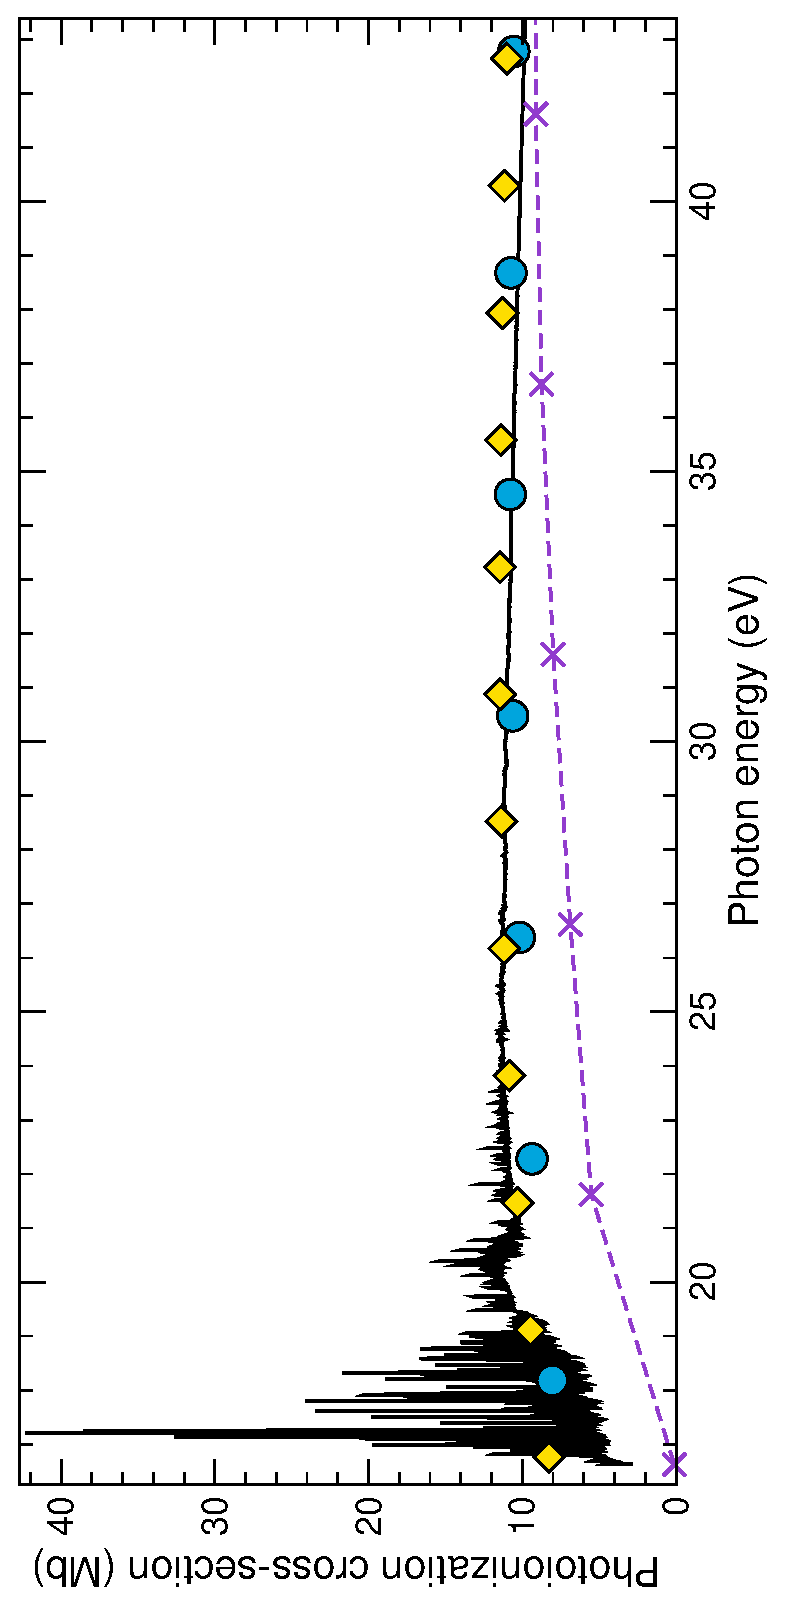
\includegraphics[scale=0.83, angle=-90]{Figures/Cobalt/photo/ground.eps}
\caption{Photoionization cross-sections in Mb against the photon energy in eV. The solid black curve is the total initial ground state, statistically weighted 3d$^8$ $^3$F to all allowed dipole final states. The crosses are results from \citet{1979ApJS...40..815R}, the diamonds are from \citet{1993ADNDT..55..233V}, and finally the circles are those from the distorted wave calculation. \citep{2015JPhB...48n4014F} \label{fig:co_ground}}
\end{sidewaysfigure}
%%%%
%%%
%%
%

%
%%
%%%
%%%%
\begin{sidewaysfigure}
\centering
\includegraphics[scale=0.83, angle=-90]{Figures/Cobalt/photo/meta.eps}
\caption{Photoionization cross-sections in Mb against the photon energy in eV. The solid black curve is the photoionization, statistically averaged levels of 3d$^7$4s $^5$F to all allowed dipole final states. The crosses are results from \citet{1979ApJS...40..815R}. \label{fig:co_excited}}
\end{sidewaysfigure}
%%%%
%%%
%%
%

In Figure \ref{fig:co_ground} we present the photoionization cross-section representing the statistically weighted initial state 3d$^8$ a$^3$F to all allowed final states. The results in this figure have been convoluted with a 10 meV Gaussian profile at full-width half-maximum to better compare with experimental results when possible. We directly compare here with the results of all three previously mentioned theoretical methods \citep{1979ApJS...40..815R, 1993ADNDT..55..233V, 2015JPhB...48n4014F}. Previous methods do not include autoionization states and therefore only background cross-sections are presented. It is clear however that the results are in excellent agreement, with only \citet{1979ApJS...40..815R} reaching factors of two or more difference in the $< 20$ eV region. As over 200 eigenenergies obtained from {\sc grasp}0 are $<$ 28 eV of photon energy, this above threshold region is dominated by multiple Rydberg resonances series converging onto these states. 

The second statistically weighted bound state a$^5$F of Co$^{+}$ is from the configuration 3d$^7$4s. In Figure \ref{fig:co_excited} we present the total photoionization cross-section for this metastable level and compare with the earlier work of \citet{1979ApJS...40..815R}. 
This cross-section is weighted as a consequence of its five fine-structure split levels $1 < J < 5$. Again, the photoionization of the $3d$ electron is favourable, so we expect the majority of the spectrum to be accounted for from the 3d$^6$4s target states, which are accessible at 5.75762 eV above the ionization threshold. Good agreement is found between the two calculations for the background cross-section, particularly in the higher photon energy range above 25 eV.

Finally, we often want to determine the partial contribution arising from the recombination process as outlined in Section \ref{sec:spe_rranddr}. We therefore use our photoionization cross-sections and convert them to recombination cross-sections following equation (\ref{eq:spe_milne}) to obtain unified RR+DR rate coefficients defined by equation (\ref{eq:spe_formalrate}). The photoionization from the lowest three initial bound states to the ground 3d$^7$  a$^4$F$_{9/2}$ are provided in Figure \ref{fig:co_rates} a), alongside their respective recombination rates, as a function of electron temperature in Figure \ref{fig:co_rates} b). While we do not carry out any radiative transport calculation involving these rates, it is in our interest to provide such analysis in the future.

%
%%
%%%
%%%%
\begin{sidewaysfigure}
\centering
\begin{subfigure}{0.45\textwidth}
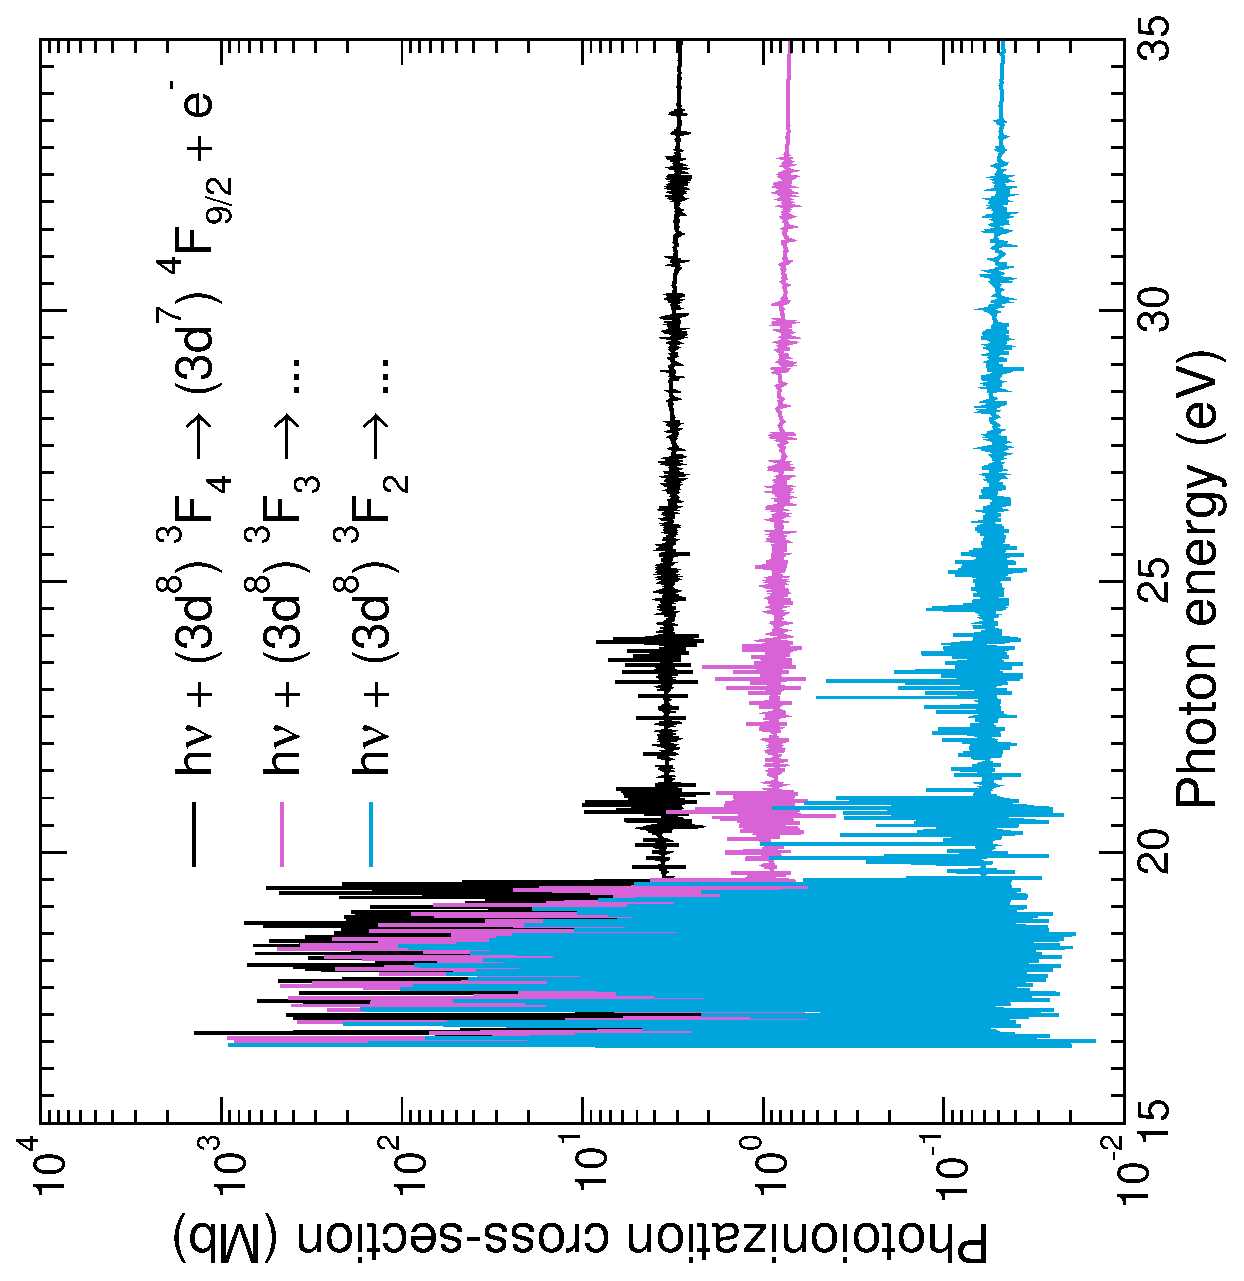
\includegraphics[scale=0.5, angle=-90]{Figures/Cobalt/recomb/recomb_photo.eps}    \end{subfigure}
    ~ %add desired spacing between images, e. g. ~, \quad, \qquad, \hfill etc. 
      %(or a blank line to force the subfigure onto a new line)
    \begin{subfigure}{0.45\textwidth}
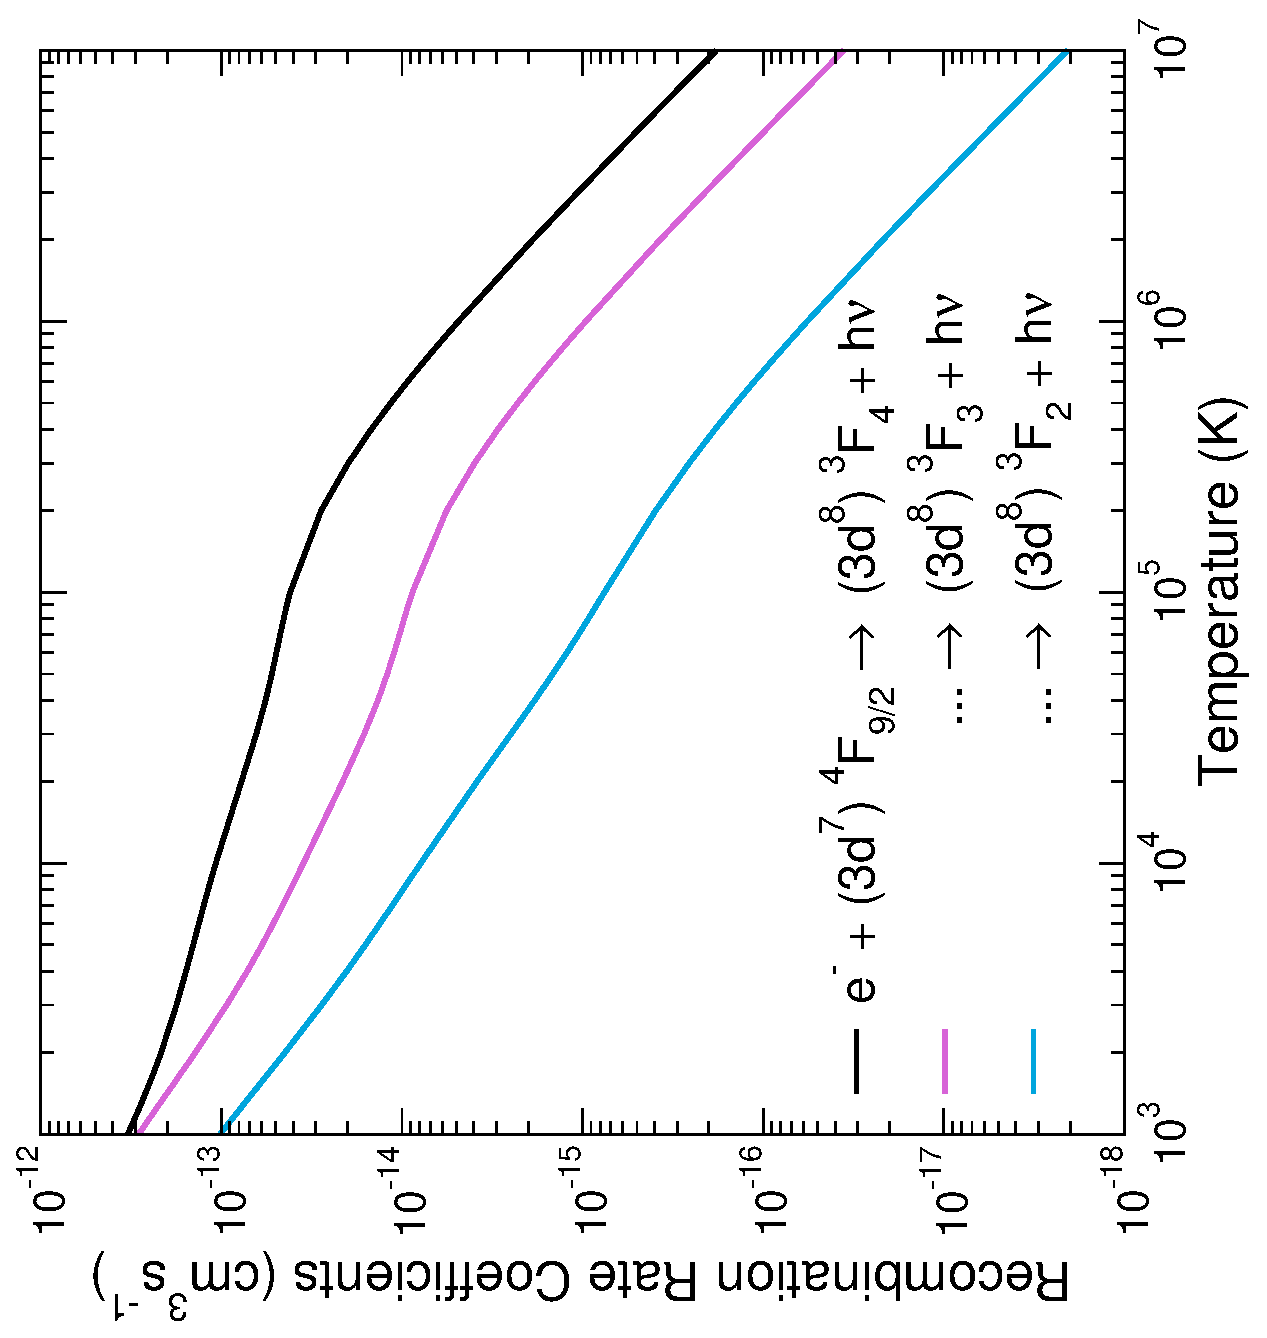
\includegraphics[scale=0.5, angle=-90]{Figures/Cobalt/recomb/total.eps}
    \end{subfigure}
\caption{We present the photoionization cross-section as a function of the photon energy in eV. Three transitions are provided, corresponding to contribution from the lowest three initial bound states into the final ground state 3d$^7$ $^4$F$_{9/2}$. Also presented are the recombination rate coefficients in cm$^3$s$^{-1}$ as a function of electron temperature in K. The transitions are from the initial  3d$^7$ $^4$F$_{9/2}$ state into the three lowest bound states. \label{fig:co_rates}}
\end{sidewaysfigure}
%%%%
%%%
%%
%

\newpage

\subsection{Electron-impact excitation}
The procedures outlined in Section \ref{sec:co_electron} are now applied to obtain accurate collision strengths and the corresponding effective collision strengths describing the electron-impact excitation of Co$^{2+}$. There has been work carried out recently on both singly ionized Co$^{+}$ \citep{2016MNRAS.456.1974S} and also Co$^{2+}$ \citep{2016MNRAS.tmp..556S}. The work of \citet{2016MNRAS.tmp..556S} is similar to our current evaluation, but differences are evident in the method considered. Their basis set has been optimized using {\sc autostructure}, and also includes a $4\bar{d}$ orbital plus additional configuration-interaction. However, only a total of 109 fine-structure levels have been included in the close coupling target representation. The semi-relativistic Breit-Pauli $R$-matrix approach was considered during the scattering calculation.

It is necessary to obtain a level of convergence in the spectra of collision strengths by applying a mesh with incremental step sizes in electron energy until convergence is achieved. Initially 5,000 equally spaced energy points were considered and it was found by the time we had reached 40,000 energy points, the $\Upsilon$'s had converged for these low lying forbidden transitions among the 292 levels. We present in Figure \ref{fig:co_adfcomp} the ratio of these $\Upsilon$'s between a mesh size of 20,000 and 40,000 energy points for level indices lower than 40 and three select temperatures, $T=3,980$ K, $T=10,000$ K, and $T=39,800$ K. The $\%$ difference is $\approx$ 2.7\% between the lowest 40 levels, and $\approx$ 3.34\% between the lowest 100 levels. 

 To extend the energy region we incorporated an additional coarse mesh above the last valence threshold. Due to the long range nature of the Coulomb potential, further contributions to the collision strengths arise from the higher partial waves, particularly for the dipole allowed lines. We compute these additional contributions using the \citet{1992A&A...254..436B} sum rule as well as a geometric series for the long-range non-dipole transitions. Hence, converged total collision strengths were accurately generated for all 42,486 transitions among the 292 fine-structure levels included in the collision calculation. The corresponding effective collision strengths were obtained by averaging these finely resolved collision strengths over a Maxwellian distribution of electron velocities for electron temperatures ranging from 3,800 to 40,000 K.  

%
%%
%%%
%%%%
\begin{figure}[hbt]
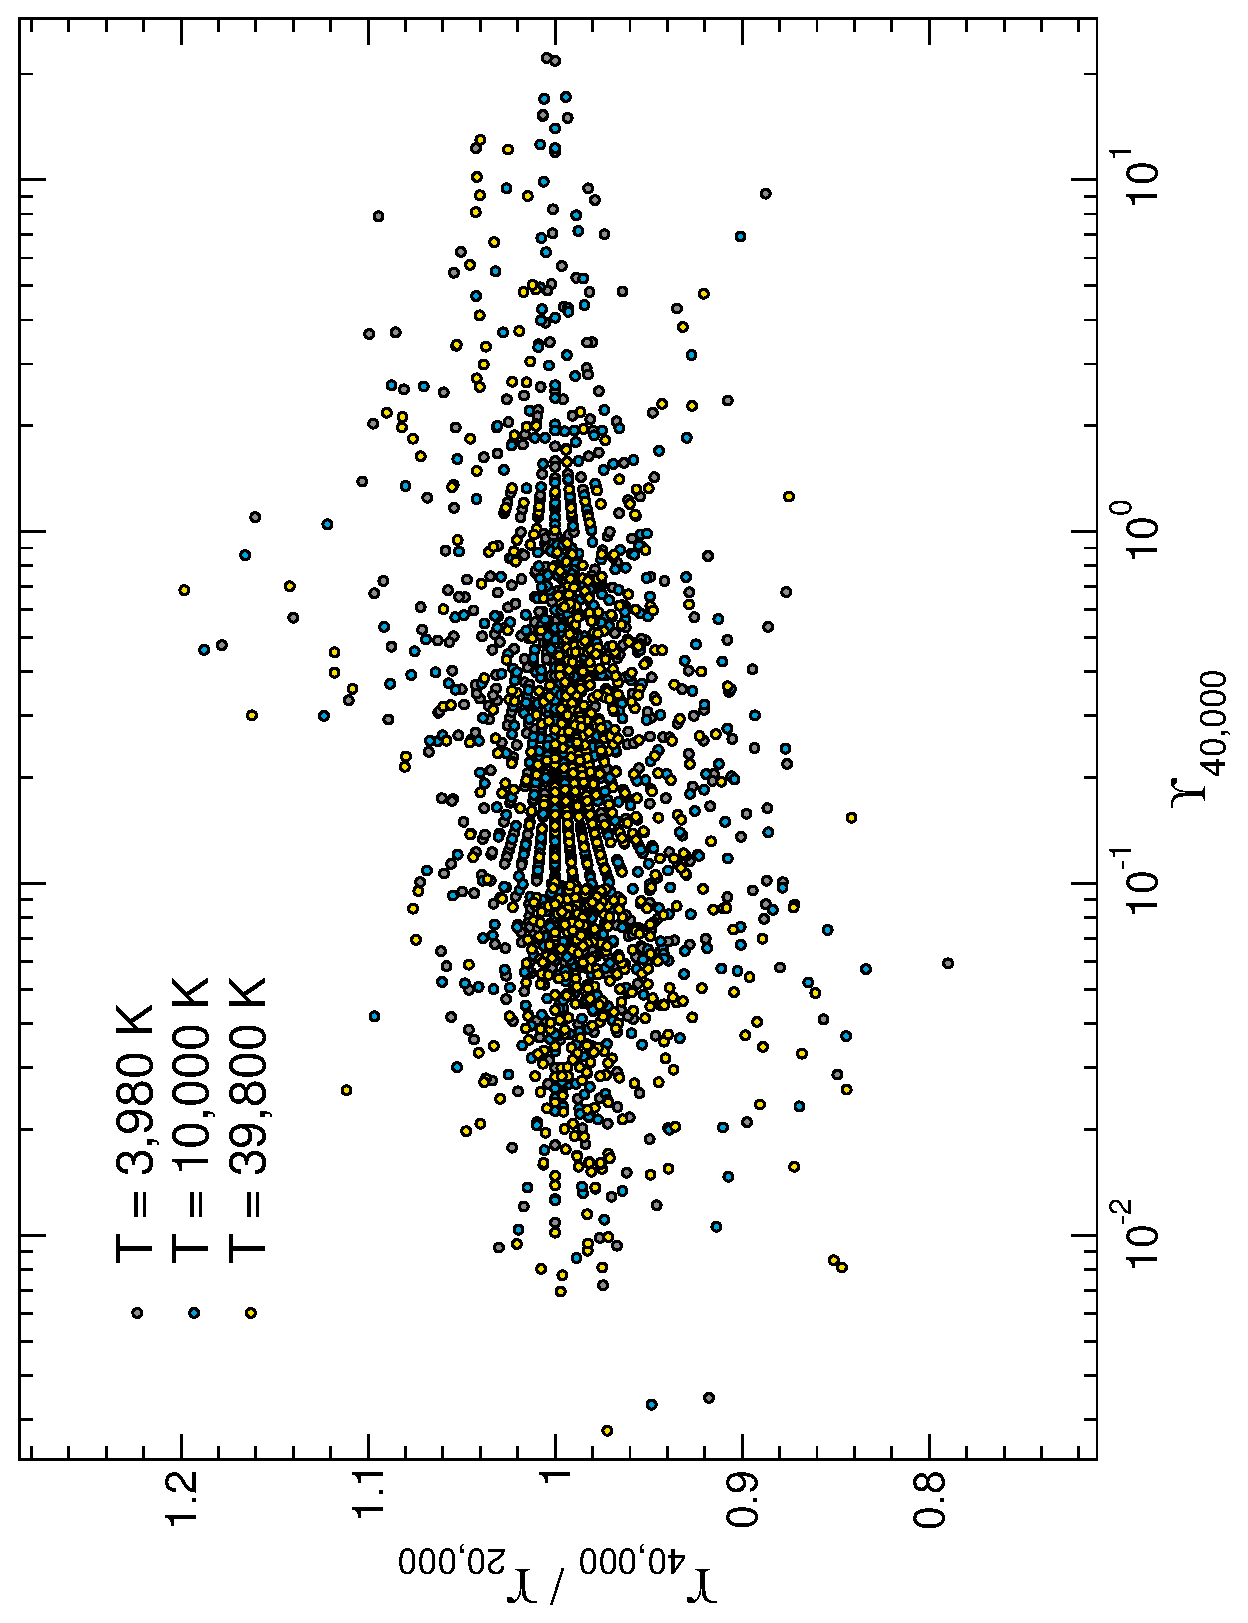
\includegraphics[scale=0.52, angle=-90]{Figures/Cobalt/mesh/adf_compare.eps}
\caption{We present the ratio of effective collision strengths $\Upsilon_{40,000}/\Upsilon_{20,000}$ as a function of the original $\Upsilon_{40,000}$ values. All transitions with level index less than 40 are plotted for three select temperatures of $T=3,980$ K, $T=10,000$ K and $T=39,800$ K. \label{fig:co_adfcomp}}
\end{figure}
%%%%
%%%
%%
%

We present the resulting collision strengths and effective collision strengths for a selection of the forbidden near infrared transitions involving the fine-structure split levels of the $^4$F ground state of Co$^{2+}$. Figure \ref{fig:co_coll_infra1} represents the transition from level 1$\rightarrow$ 2, Figure \ref{fig:co_coll_infra2} is transition $1 \rightarrow 3$, and Figure Figure \ref{fig:co_coll_infra3} is the transition $2 \rightarrow 3$. The collision strength is strongest here for $\Omega_{1 \rightarrow 2}$ due to the $\Delta J = 0$ partial wave. Comparison of the effective collision strengths are made for each transition with the work of \citet{2016MNRAS.tmp..556S} and good agreement is found for all temperatures above 10,000 K. For temperatures below this value the two calculations deviate somewhat, most probably due to the differing resonance profiles converging onto differing threshold positions. The present calculation has shifted the thresholds to lie in their exact observed positions listed in Table \ref{tab:co_energy} whereas the \citet{2016MNRAS.tmp..556S} evaluations do not mention any adjustments.

%
%%
%%%
%%%%
\begin{sidewaysfigure}
\centering
\includegraphics[scale=0.75, angle=-90]{Figures/Cobalt/electron/trans1.eps}
\caption{The collision strength $\Omega_{1\rightarrow 2}$ is presented as a function of electron energy in eV. Also presented are the corresponding effective collision strengths as a function of temperature in K. Solid black lines with squares are the current data set and the dashed blue line with triangles represent the results from \citet{2016MNRAS.tmp..556S}. \label{fig:co_coll_infra1}}
\end{sidewaysfigure}
%%%%
%%%
%%
%

%
%%
%%%
%%%%
\begin{sidewaysfigure}
\centering
\includegraphics[scale=0.75, angle=-90]{Figures/Cobalt/electron/trans2.eps}
\caption{The collision strength $\Omega_{1\rightarrow 3}$ is presented as a function of electron energy in eV. Also presented are the corresponding effective collision strengths as a function of temperature in K. Solid black lines with squares are the current data set and the dashed blue line with triangles represent the results from \citet{2016MNRAS.tmp..556S}. \label{fig:co_coll_infra2}}
\end{sidewaysfigure}
%%%%
%%%
%%
%

%
%%
%%%
%%%%
\begin{sidewaysfigure}
\centering
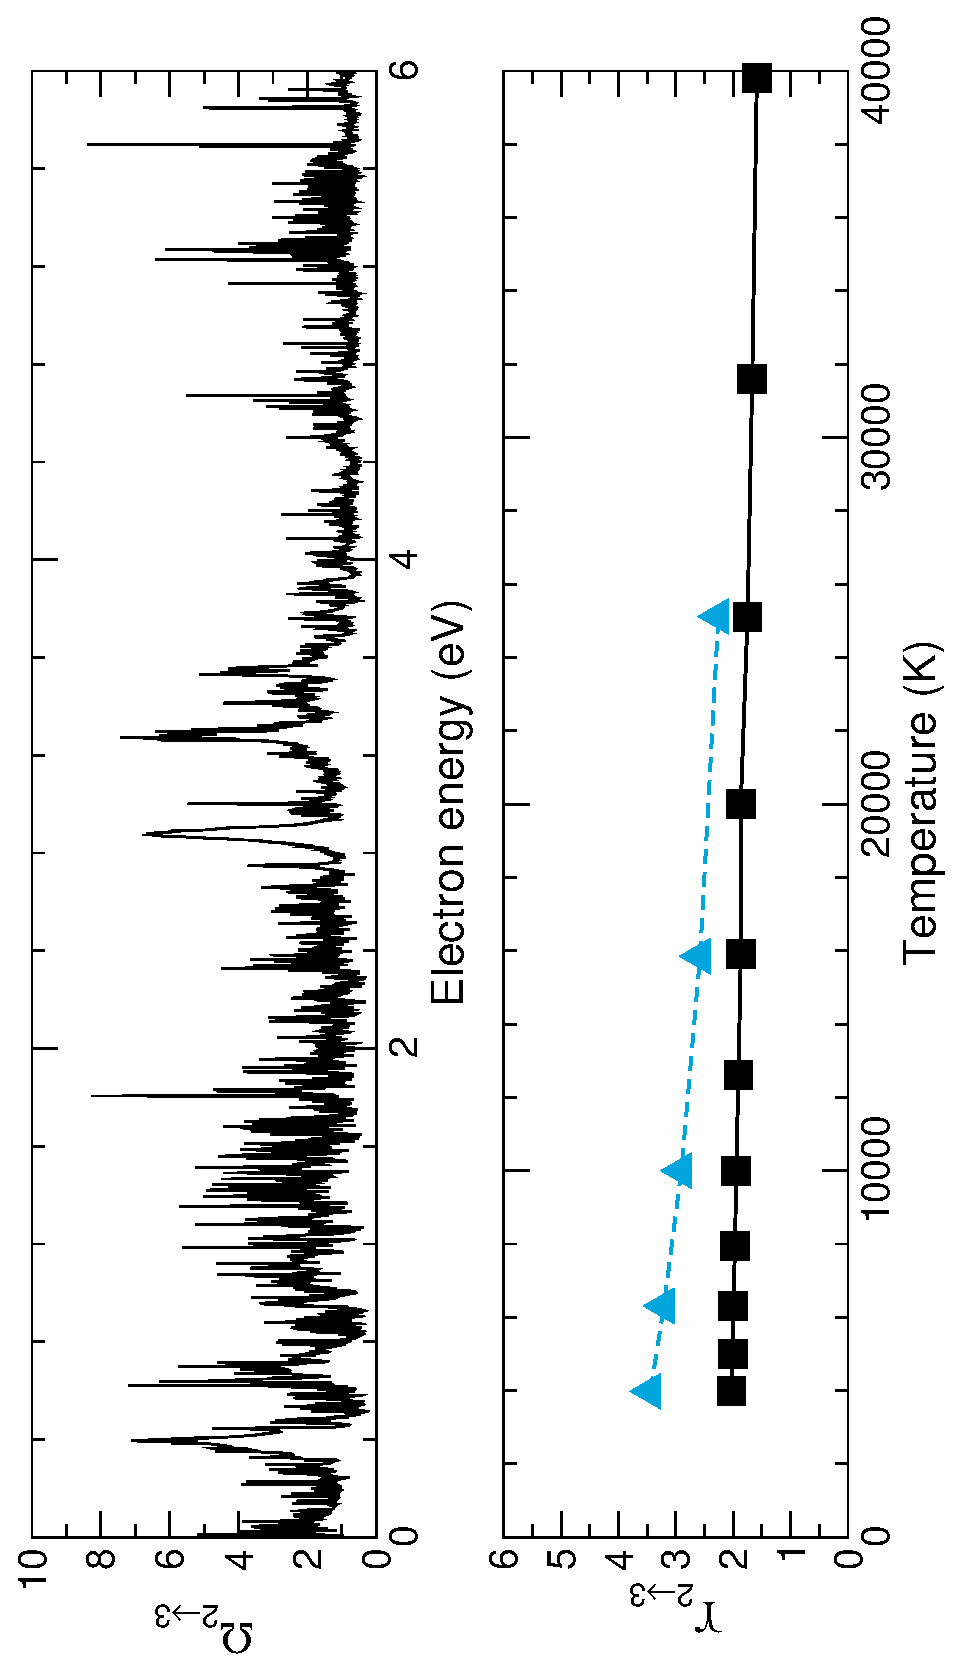
\includegraphics[scale=0.75, angle=-90]{Figures/Cobalt/electron/trans4.eps}
\caption{The collision strength $\Omega_{2\rightarrow 3}$ is presented as a function of electron energy in eV. Also presented are the corresponding effective collision strengths as a function of temperature in K. Solid black lines with squares are the current data set and the dashed blue line with triangles represent the results from \citet{2016MNRAS.tmp..556S}. \label{fig:co_coll_infra3}}
\end{sidewaysfigure}
%%%%
%%%
%%
%

In Figure \ref{fig:co_coll_5to7} we present the effective collision strengths for some higher lying transitions, the 3d$^7$ $^4$F$_{9/2}$ - 3d$^7$ $^2$G$_{9/2}$ (1 $\rightarrow$ 8), 3d$^7$ $^2$P$_{1/2}$ - 3d$^7$ $^2$H$_{9/2}$ (11 $\rightarrow$ 13) and 3d$^7$ $^2$G$_{7/2}$ - 3d$^7$ $^2$H$_{9/2}$ (9 $\rightarrow$ 13). Excellent agreement is evident for all three transitions when a comparison is made with the data of \citet{2016MNRAS.tmp..556S} across all temperatures where a comparison is possible. We present in Table \ref{tab:co_ups} the effective collision strengths for all transitions among the lowest 10 3d$^7$ fine-structure levels across eight temperatures of astrophysical importance.

%
%%
%%%
%%%%
\begin{figure}
\centering
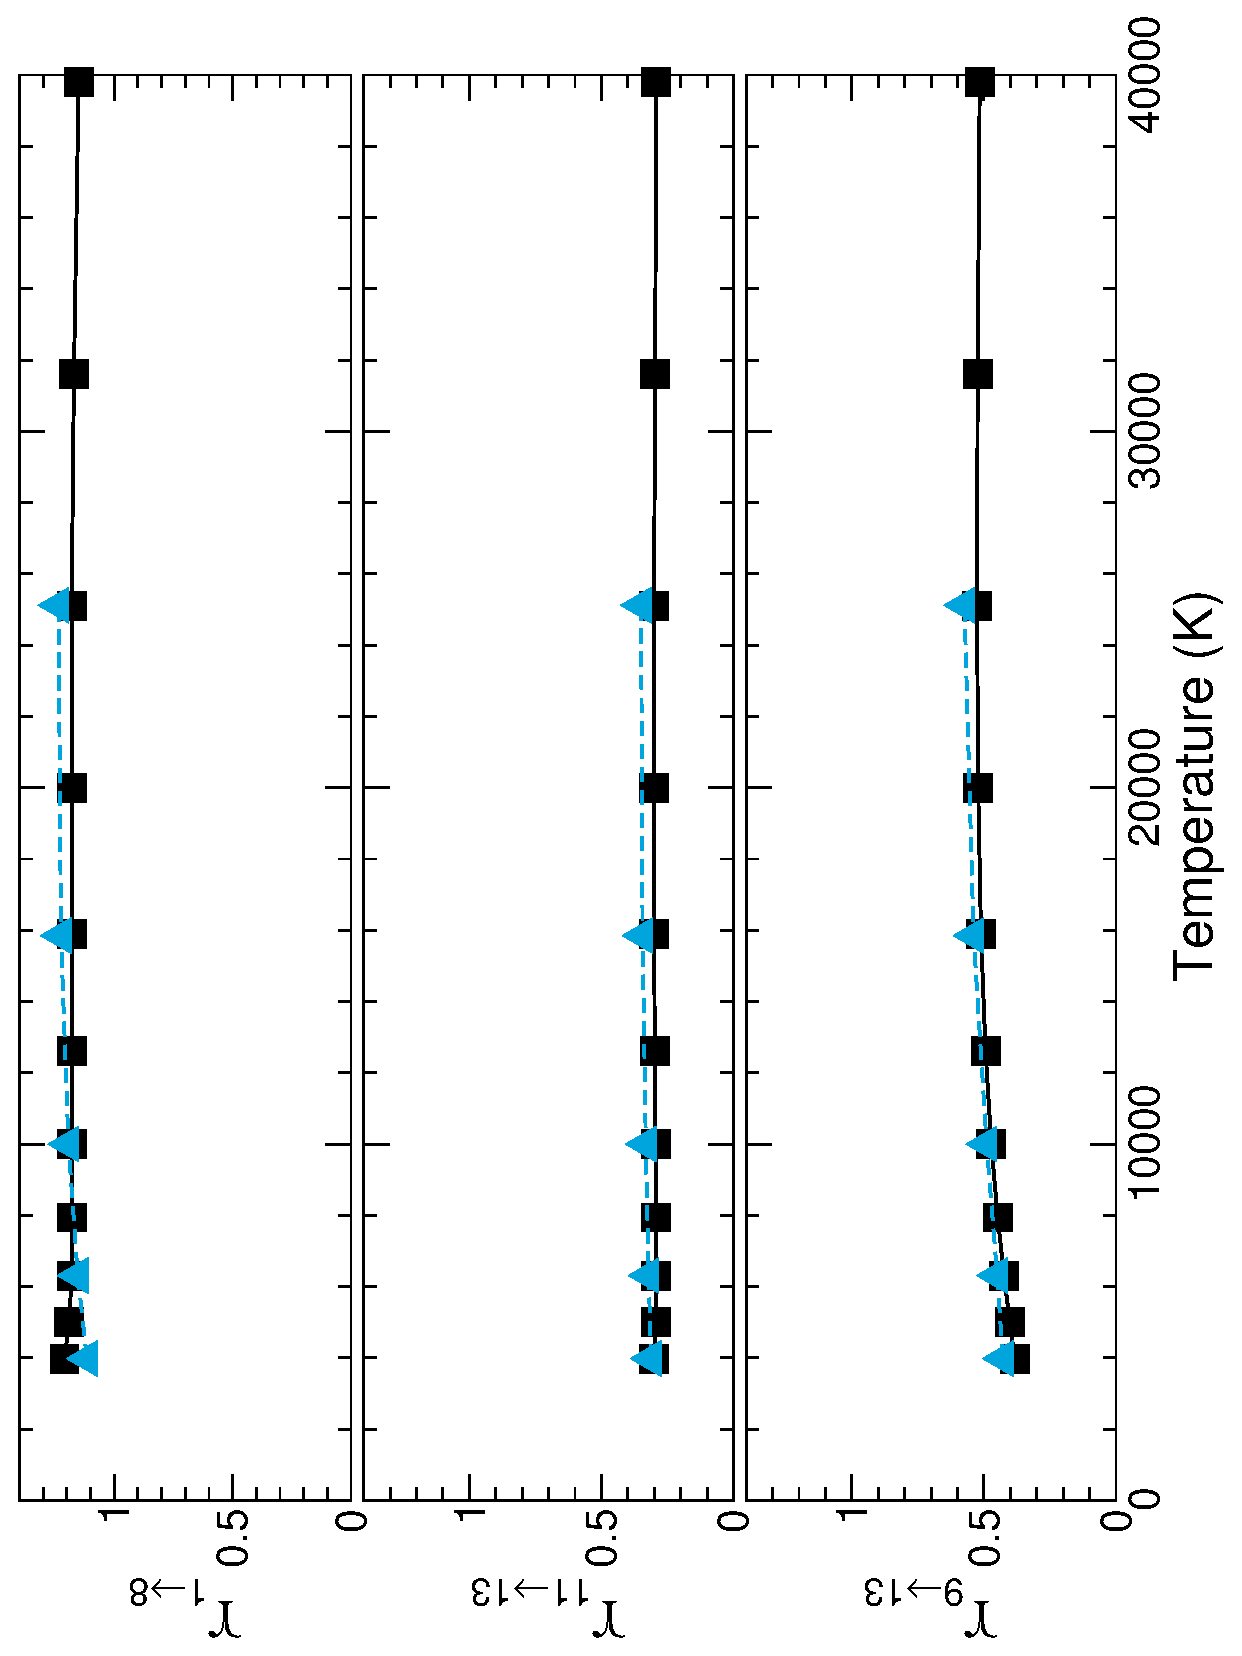
\includegraphics[scale=0.53, angle=-90]{Figures/Cobalt/electron/trans5-7.eps}
\caption{The effective collision strengths, $\Upsilon_{1\rightarrow 8}$ (top), $\Upsilon_{11\rightarrow 13}$ (middle) and $\Upsilon_{9\rightarrow 13}$ (bottom), presented as a function of temperature in K (bottom). Solid black lines with squares are the current data set and the dashed blue line with triangles represent the results from \citep{2016MNRAS.tmp..556S}. \label{fig:co_coll_5to7}}
\end{figure}
%%%%
%%%
%%
%

While we do not compare with the next set of results, we are still able to provide the lowest dipole allowed transitions for completeness, and show the effect from the top-up procedure. In Figure \ref{fig:co_dipole} we present the effective collision strength for the transitions 3d$^6$4p $^6$D$^{{\rm o}}_{9/2} \rightarrow$ 3d$^6$4s $^6$D$_{9/2}$, 3d$^6$4p $^4$D$^{{\rm o}}_{7/2} \rightarrow$ 3d$^7$ $^4$F$_{9/2}$, 3d$^6$4p $^4$D$^{{\rm o}}_{3/2} \rightarrow$ 3d$^7$ $^2$P$_{1/2}$, and 3d$^6$4p $^2$H$^{{\rm o}}_{11/2} \rightarrow$ 3d$^6$4s $^2$H$_{13/2}$ both with (dashed blue), and without (solid black) contribution from top-up. The first transition has a large contribution due to top-up as the quantum numbers are unchanged between initial and final state, $\Delta S = 0$, $\Delta L = 0$, and $\Delta J = 0$. Other transitions have little or no change in their total effective collision strength, but generally any differences occur at temperatures that are beyond the scope of this investigation, i.e. $T>30,000$ K.

\newpage

%
%%
%%%
%%%%
\begin{figure}
\includegraphics[scale=0.59, angle=-90]{Figures/Cobalt/electron/dipole.eps}
\caption{We present the effective collision strengths according to $\Upsilon_{65\rightarrow 18}$ (top left), $\Upsilon_{81\rightarrow 1}$ (top right), $\Upsilon_{86\rightarrow 11}$ (bottom left), and $\Upsilon_{120\rightarrow 30}$ (bottom right), as a function of electron temperature in K. The solid black curves represent the contribution from the first $J=13$ partial waves (no top-up included) and the dashed blue curves represent the contribution from the remaining partial waves up to $J=38$ (top-up included). \label{fig:co_dipole}}
\end{figure}
%%%%
%%%
%%
%

\subsection{Collisional radiative modelling}\label{sec:co_radiative}
Combining the electron-impact excitation rates with the decay rates ($A$-values), it is possible to study important infrared and visible line ratios from the computer code {\sc collr-v1.0} detailed in Chapter \ref{cha:spectral}. For simplicity and purpose of this study, we neglect the recombination and ionization processes from the neighbouring ion stages and focus on the populating mechanisms solely of Co$^{2+}$.

It is possible to calculate the populations, which are functions of both electron temperature and density, for each of the 262 levels. Due to this quasi-static equilibrium approach $N_1$ is unknown, but since the remaining populations are all relative to $N_1$, we can choose the value to be $1,000$ for example. Populations 2 - 7 are shown in Figure \ref{fig:co_populations} for $T=4,170$, and $T=7,590$, and three densities per temperature; $N_e = 10^4$cm$^{-3}$, $N_e = 10^6$cm$^{-3}$ and $N_e = 10^8$cm$^{-3}$. This reinforces that the problem is not trivial, and the $\Upsilon$'s and $A$-values are of utmost importance.

%
%%
%%%
%%%%
\begin{sidewaysfigure}
\centering
\begin{subfigure}{0.45\textwidth}
\includegraphics[scale=0.48, angle=-90]{Figures/Cobalt/modelling/populations/population1.eps}    \end{subfigure}
    ~ %add desired spacing between images, e. g. ~, \quad, \qquad, \hfill etc. 
      %(or a blank line to force the subfigure onto a new line)
    \begin{subfigure}{0.45\textwidth}
\includegraphics[scale=0.48, angle=-90]{Figures/Cobalt/modelling/populations/population2.eps} 
    \end{subfigure}
\caption{We plot the populations 2 - 7 for $T=4,170$ K (left) and $T=7,590$ K (right) as a function of the target state energies in eV provided by Table \ref{tab:co_energy}, and $N_1 = 1,000$. The populations for each temperature are plotted for three electron densities $N_e = 10^4$cm$^{-3}$, $N_e = 10^6$cm$^{-3}$ and $N_e = 10^8$cm$^{-3}$. \label{fig:co_populations}}
\end{sidewaysfigure}
%%%%
%%%
%%
%

%
%%
%%%
%%%%
\begin{figure}[h]
\centering
\includegraphics[scale=0.62, angle=0]{Figures/Cobalt/modelling/population2-v2}
\caption{We present the surface plot of $N_2$ in terms of $N_1$ for logarithmic grids of the electron density (cm$^3$) and temperature (K). The resulting population is the corresponding $z$-axis. \label{fig:co_pop2}}
\end{figure}
%%%%
%%%
%%
%
It is also possible to plot particular populations as functions of both electron temperature and density to explain the features in Figure \ref{fig:co_populations}. We therefore present in Figure \ref{fig:co_pop2} the results for a particular population, $N_2$, where we can clearly see the effect of these varying parameters. 

A more useful property to consider is the line ratio as defined in equation (\ref{eq:spe_lratio}). We can therefore investigate select transitions that have been suggested as temperature or density diagnostics. 
%We define the line ratio as
%\[
%\frac{N_j A_{j\rightarrow i}}{N_kA_{k\rightarrow m}},
%\]
%where the populations of the $n^{th}$ level as a function of the ground state are given by $N_n$, and the decay rates are the results from Section \ref{sec:co_target}.

Figure \ref{fig:co_consttemp} depicts the results of the line ratio [0.66$\mu$m]/[0.69$\mu$m] which corresponds to the transitions,
\[
\frac{I_{5\rightarrow1}[0.66\mu m]}{I_{6\rightarrow2}[0.69\mu m]} = \frac{3\text{d}^7 ~\text{a}^4\text{P}_{5/2}\rightarrow 3\text{d}^7 ~\text{a}^4\text{F}_{9/2}}{3\text{d}^7 ~\text{a}^4\text{P}_{3/2} \rightarrow 3\text{d}^7 ~\text{a}^4\text{F}_{7/2}},
\]
as a function of electron density for particular temperatures. The dashed line provides the lowest temperature, $T = 3,980$ K, with increasing $T$ to $T = 5,010$ K, $T = 6,310$ K and $T = 7,940$ K. The line ratio is constant for densities $N_e < 10^{4}$ cm$^{-3}$ and also $N_e > 10^{7}$ cm$^{-3}$ for the temperatures considered. This could be considered a useful diagnostic for densities in the range of $10^{4}$ cm$^{-3}$ $< N_e < 3\times10^{5}$ cm$^{-3}$ where it remains constant for increasing temperatures before it reaches its minimum $\approx 5\times 10^{5}$ cm$^{-3}$. We have also shown the results of the low and high electron density limits from equations (\ref{eq:spe_coronal}) and (\ref{eq:spe_lte}) respectively. The coronal approximation is not as accurate (crosses), but we can see that applying a constant shift in the $y$-axis (stars) that it is useful in determining the actual separation between line ratios. 

%
%%
%%%
%%%%
\begin{figure}[h]
\includegraphics[scale=0.54, angle=-90]{Figures/Cobalt/modelling/5-1over6-2/const_temp.eps}
\caption{The line ratio [0.66$\mu$m]/[0.69$\mu$m] as a function of electron density (cm$^{-3}$). The dashed curve is the lowest temperature, $T = 3,980$ K. The remaining solid black curves are for temperatures $T = 5,010$ K, $T = 6,310$ K, and $T = 7,940$ K for decreasing line ratio. The crosses represent the coronal (low density) and LTE (high density) limits for each of the four temperatures. \label{fig:co_consttemp}}
\end{figure}
%%%%
%%%
%%
%

Next we consider lines suggested by \citet{1995ASPC...78..291R}, (around the wavelength region 6,000 - 6,500 {\rm \AA}) to be applied as density diagnostics. At 10,000 K, we can see the photon emissivity coefficients of the $8\rightarrow 1$ and $8\rightarrow 2$ lines becomes more dominant for increasing temperatures, and they are also in this ideal wavelength region. \citet{2015ApJ...798...93T} also suggests the $2\rightarrow 1$, 11.88$\mu$m as a useful diagnostic line. We finally present the results of three line ratios,
\[
\frac{I_{2\rightarrow 1}[11.88\mu {\rm m}]}{I_{5\rightarrow 1}[0.66\mu {\rm m}]} = \frac{3\rm{d}^7 ~\rm{a}^4\rm{F}_{7/2} \rightarrow 3\rm{d}^7 ~\rm{a}^4\rm{F}_{9/2}}{3\rm{d}^7 ~\rm{a}^4\rm{P}_{5/2} \rightarrow 3\rm{d}^7 ~\rm{a}^4\rm{F}_{9/2}},
\]
\[
\frac{I_{2\rightarrow 1}[11.88\mu {\rm m}]}{I_{8\rightarrow 1}[0.59\mu {\rm m}]} = \frac{3\rm{d}^7 ~\rm{a}^4\rm{F}_{7/2} \rightarrow 3\rm{d}^7 ~\rm{a}^4\rm{F}_{9/2}}{3\rm{d}^7 ~\rm{a}^2\rm{G}_{9/2} \rightarrow 3\rm{d}^7 ~\rm{a}^4\rm{F}_{9/2}},
\]
\[
\frac{I_{2\rightarrow 1}[11.88\mu {\rm m}]}{I_{8\rightarrow 2}[0.62\mu {\rm m}]} = \frac{3\rm{d}^7 ~\rm{a}^4\rm{F}_{7/2} \rightarrow 3\rm{d}^7 ~\rm{a}^4\rm{F}_{9/2}}{3\rm{d}^7 ~\rm{a}^2\rm{G}_{9/2} \rightarrow 3\rm{d}^7 ~\rm{a}^4\rm{F}_{7/2}},
\]


%
%%
%%%
%%%%
\begin{sidewaysfigure}
\centering
\includegraphics[scale=0.8, angle=-90]{Figures/Cobalt/modelling/lineratio_new.eps}
\caption{Three line ratios of [11.88$\mu$m]/[0.66$\mu$m] (left), [11.88$\mu$m]/[0.59$\mu$m] (middle), and [11.88$\mu$m]/[0.62$\mu$m] (right) as a function of electron temperature (K). The red, dashed curve is the lowest density, $N_e = 10^2$ cm$^{-3}$. The remaining solid black curves are for temperatures $N_e = 10^3$ cm$^{-3}$, $N_e = 10^4$ cm$^{-3}$, $N_e = 10^5$ cm$^{-3}$, and $N_e = 10^6$ cm$^{-3}$ for decreasing line ratio.\label{fig:co_constdens}}
\end{sidewaysfigure}
%%%%
%%%
%%
%


We plot in Figure \ref{fig:co_constdens} the three line ratios as a function of electron temperature. The red dashed curves are the lowest electron density in each Figure - $N_e = 10^2$ cm$^{-3}$, and the remaining solid curves correspond to $N_e = 10^3$ cm$^{-3}$, $N_e = 10^4$ cm$^{-3}$, $N_e = 10^5$ cm$^{-3}$, and $N_e = 10^6$ cm$^{-3}$. Each line ratio is a varying function of increasing temperature across the range of interest. The three lowest densities lie right on top of each other in each plot, and therefore they provide useful diagnostics for this density range. As $N_e > 10^5$ cm$^{-3}$, the line ratio begins to diverge, and even becomes constant for larger densities.

\newpage
\section{Conclusion}\label{sec:co_conclusions}
In this Chapter we present an extensive set of atomic data for the photoionization of Co$^{+}$ and the electron-impact excitation of Co$^{2+}$. Initially we have exploited the computer code {\sc grasp}0 to obtain a description of the atomic wavefunctions and generate energy levels for the 292 fine-structure bound target states and the corresponding $A$-values for transitions between these levels. We compare these levels with the theoretical work of \citet{2016MNRAS.tmp..556S} and the observational study of \citet{1985aeli.book.....S}, which are the values recorded in the NIST database. Furthermore, the {\sc darc} computer package has been employed to extend the problem to include photon and electron interactions. 

We then present statistically weighted, level-resolved ground and metastable photoionization cross-sections for the Co$^{+}$ ion as well as collision strengths and Maxwe-\\llian averaged effective collision strengths describing the electron-impact excitation of the Co$^{2+}$ ion. Comparisons are made with other works where possible and good agreement is found. The reliability of the atomic data presented has been rigorously tested through a variety of means, such as the sophistication of the current calculations where great care has been taken to ensure the inclusion of important correlation and configuration-interaction in the wavefunction expansions. In addition the complex resonance structures in the cross-sections (photoionization and excitation) have been accurately resolved through a series of calculations incorporating mesh sizes with finer and finer energy increments. A proper consideration was also taken of the contributions from the high partial waves to ensure convergence of the collision strengths for the allowed transitions in particular. A conclusive assessment of the accuracy of the presented Maxwellian averaged collision strengths will necessarily come from any subsequent astrophysical or diagnostic application. 

In Section \ref{sec:co_radiative} the electron-impact excitation rates were combined with the decay rates ($A$-values) to investigate important infrared and visible line ratios. During this process we were able to identify useful transitions that could be used as temperature and/or density sensitive diagnostic lines.

\newpage
\begin{table*}
\centering
\footnotesize
\begin{tabular}{c c c c c c c c c c}
\toprule
\multicolumn{2}{c}{ } & \multicolumn{8}{c}{log $T$ (K)} \\
$i$ & $j$   & 3.6 & 3.7 & 3.8 & 3.9 &  4 & 4.1 & 4.2 & 4.3 \\%& 4.4 \\
\midrule
   1 &    2 & $ 2.92^{+00}$ & $ 2.90^{+00}$ & $ 2.86^{+00}$ & $ 2.82^{+00}$ & $ 2.77^{+00}$ & $ 2.70^{+00}$ & $ 2.63^{+00}$ & $ 2.54^{+00}$ \\%& $ 2.44^{+00}$\\
   1 &    3 & $ 9.24^{-01}$ & $ 9.36^{-01}$ & $ 9.41^{-01}$ & $ 9.37^{-01}$ & $ 9.26^{-01}$ & $ 9.06^{-01}$ & $ 8.79^{-01}$ & $ 8.45^{-01}$ \\%& $ 8.06^{-01}$\\
   2 &    3 & $ 2.02^{+00}$ & $ 2.01^{+00}$ & $ 1.99^{+00}$ & $ 1.97^{+00}$ & $ 1.94^{+00}$ & $ 1.91^{+00}$ & $ 1.86^{+00}$ & $ 1.81^{+00}$ \\%& $ 1.74^{+00}$\\ 
   1 &    4 & $ 3.17^{-01}$ & $ 3.23^{-01}$ & $ 3.26^{-01}$ & $ 3.25^{-01}$ & $ 3.21^{-01}$ & $ 3.13^{-01}$ & $ 3.03^{-01}$ & $ 2.90^{-01}$ \\%& $ 2.75^{-01}$\\
   2 &    4 & $ 7.46^{-01}$ & $ 7.65^{-01}$ & $ 7.77^{-01}$ & $ 7.80^{-01}$ & $ 7.76^{-01}$ & $ 7.64^{-01}$ & $ 7.43^{-01}$ & $ 7.17^{-01}$ \\%& $ 6.85^{-01}$\\
   3 &    4 & $ 1.42^{+00}$ & $ 1.42^{+00}$ & $ 1.42^{+00}$ & $ 1.42^{+00}$ & $ 1.40^{+00}$ & $ 1.39^{+00}$ & $ 1.36^{+00}$ & $ 1.32^{+00}$ \\%& $ 1.28^{+00}$\\
   1 &    5 & $ 1.16^{+00}$ & $ 1.16^{+00}$ & $ 1.17^{+00}$ & $ 1.19^{+00}$ & $ 1.20^{+00}$ & $ 1.21^{+00}$ & $ 1.21^{+00}$ & $ 1.20^{+00}$ \\%& $ 1.19^{+00}$\\
   2 &    5 & $ 8.11^{-01}$ & $ 8.03^{-01}$ & $ 8.02^{-01}$ & $ 8.07^{-01}$ & $ 8.13^{-01}$ & $ 8.17^{-01}$ & $ 8.15^{-01}$ & $ 8.05^{-01}$ \\%& $ 7.89^{-01}$\\
   3 &    5 & $ 5.72^{-01}$ & $ 5.60^{-01}$ & $ 5.53^{-01}$ & $ 5.51^{-01}$ & $ 5.50^{-01}$ & $ 5.48^{-01}$ & $ 5.43^{-01}$ & $ 5.33^{-01}$ \\%& $ 5.19^{-01}$\\   
   4 &    5 & $ 3.68^{-01}$ & $ 3.51^{-01}$ & $ 3.37^{-01}$ & $ 3.27^{-01}$ & $ 3.20^{-01}$ & $ 3.13^{-01}$ & $ 3.06^{-01}$ & $ 2.98^{-01}$ \\%& $ 2.88^{-01}$\\    
   1 &    6 & $ 4.84^{-01}$ & $ 4.82^{-01}$ & $ 4.84^{-01}$ & $ 4.90^{-01}$ & $ 4.95^{-01}$ & $ 4.98^{-01}$ & $ 4.97^{-01}$ & $ 4.91^{-01}$ \\%& $ 4.82^{-01}$\\
   2 &    6 & $ 5.54^{-01}$ & $ 5.52^{-01}$ & $ 5.53^{-01}$ & $ 5.56^{-01}$ & $ 5.60^{-01}$ & $ 5.61^{-01}$ & $ 5.58^{-01}$ & $ 5.52^{-01}$ \\%& $ 5.41^{-01}$\\   
   3 &    6 & $ 4.55^{-01}$ & $ 4.51^{-01}$ & $ 4.51^{-01}$ & $ 4.54^{-01}$ & $ 4.57^{-01}$ & $ 4.59^{-01}$ & $ 4.57^{-01}$ & $ 4.52^{-01}$ \\%& $ 4.44^{-01}$\\   
   4 &    6 & $ 2.92^{-01}$ & $ 2.88^{-01}$ & $ 2.89^{-01}$ & $ 2.92^{-01}$ & $ 2.96^{-01}$ & $ 3.00^{-01}$ & $ 3.02^{-01}$ & $ 3.00^{-01}$ \\%& $ 2.96^{-01}$\\
   5 &    6 & $ 6.14^{-01}$ & $ 6.15^{-01}$ & $ 6.21^{-01}$ & $ 6.31^{-01}$ & $ 6.44^{-01}$ & $ 6.59^{-01}$ & $ 6.73^{-01}$ & $ 6.82^{-01}$ \\%& $ 6.87^{-01}$\\     
   1 &    7 & $ 1.86^{-01}$ & $ 1.85^{-01}$ & $ 1.85^{-01}$ & $ 1.86^{-01}$ & $ 1.87^{-01}$ & $ 1.86^{-01}$ & $ 1.84^{-01}$ & $ 1.81^{-01}$ \\%& $ 1.76^{-01}$\\
   2 &    7 & $ 2.03^{-01}$ & $ 2.03^{-01}$ & $ 2.06^{-01}$ & $ 2.10^{-01}$ & $ 2.15^{-01}$ & $ 2.18^{-01}$ & $ 2.19^{-01}$ & $ 2.18^{-01}$ \\%& $ 2.14^{-01}$\\
   3 &    7 & $ 2.34^{-01}$ & $ 2.36^{-01}$ & $ 2.39^{-01}$ & $ 2.43^{-01}$ & $ 2.48^{-01}$ & $ 2.51^{-01}$ & $ 2.53^{-01}$ & $ 2.52^{-01}$ \\%& $ 2.48^{-01}$\\      
   4 &    7 & $ 2.19^{-01}$ & $ 2.20^{-01}$ & $ 2.22^{-01}$ & $ 2.26^{-01}$ & $ 2.29^{-01}$ & $ 2.31^{-01}$ & $ 2.32^{-01}$ & $ 2.31^{-01}$ \\%& $ 2.28^{-01}$\\
   5 &    7 & $ 2.43^{-01}$ & $ 2.45^{-01}$ & $ 2.49^{-01}$ & $ 2.56^{-01}$ & $ 2.65^{-01}$ & $ 2.75^{-01}$ & $ 2.85^{-01}$ & $ 2.93^{-01}$ \\%& $ 2.98^{-01}$\\      
   6 &    7 & $ 2.73^{-01}$ & $ 2.72^{-01}$ & $ 2.72^{-01}$ & $ 2.74^{-01}$ & $ 2.76^{-01}$ & $ 2.79^{-01}$ & $ 2.81^{-01}$ & $ 2.83^{-01}$ \\%& $ 2.82^{-01}$\\   
   1 &    8 & $ 1.22^{+00}$ & $ 1.20^{+00}$ & $ 1.19^{+00}$ & $ 1.19^{+00}$ & $ 1.19^{+00}$ & $ 1.19^{+00}$ & $ 1.19^{+00}$ & $ 1.19^{+00}$ \\%& $ 1.18^{+00}$\\
   2 &    8 & $ 7.27^{-01}$ & $ 7.14^{-01}$ & $ 7.06^{-01}$ & $ 7.02^{-01}$ & $ 6.99^{-01}$ & $ 6.98^{-01}$ & $ 6.96^{-01}$ & $ 6.92^{-01}$ \\%& $ 6.86^{-01}$\\   
   3 &    8 & $ 3.85^{-01}$ & $ 3.76^{-01}$ & $ 3.70^{-01}$ & $ 3.65^{-01}$ & $ 3.62^{-01}$ & $ 3.59^{-01}$ & $ 3.55^{-01}$ & $ 3.51^{-01}$ \\%& $ 3.45^{-01}$\\   
   4 &    8 & $ 1.75^{-01}$ & $ 1.69^{-01}$ & $ 1.65^{-01}$ & $ 1.60^{-01}$ & $ 1.57^{-01}$ & $ 1.53^{-01}$ & $ 1.50^{-01}$ & $ 1.46^{-01}$ \\%& $ 1.43^{-01}$\\
   5 &    8 & $ 3.24^{-01}$ & $ 3.18^{-01}$ & $ 3.11^{-01}$ & $ 3.07^{-01}$ & $ 3.04^{-01}$ & $ 3.02^{-01}$ & $ 3.01^{-01}$ & $ 3.00^{-01}$ \\%& $ 2.98^{-01}$\\
   6 &    8 & $ 1.56^{-01}$ & $ 1.51^{-01}$ & $ 1.47^{-01}$ & $ 1.43^{-01}$ & $ 1.41^{-01}$ & $ 1.40^{-01}$ & $ 1.39^{-01}$ & $ 1.38^{-01}$ \\%& $ 1.37^{-01}$\\
   7 &    8 & $ 5.48^{-02}$ & $ 5.20^{-02}$ & $ 4.93^{-02}$ & $ 4.70^{-02}$ & $ 4.51^{-02}$ & $ 4.36^{-02}$ & $ 4.24^{-02}$ & $ 4.14^{-02}$ \\%& $ 4.03^{-02}$\\            
   1 &    9 & $ 3.16^{-01}$ & $ 3.10^{-01}$ & $ 3.06^{-01}$ & $ 3.05^{-01}$ & $ 3.05^{-01}$ & $ 3.04^{-01}$ & $ 3.03^{-01}$ & $ 3.01^{-01}$ \\%& $ 2.97^{-01}$\\
   2 &    9 & $ 5.02^{-01}$ & $ 4.99^{-01}$ & $ 4.99^{-01}$ & $ 5.01^{-01}$ & $ 5.05^{-01}$ & $ 5.08^{-01}$ & $ 5.11^{-01}$ & $ 5.12^{-01}$ \\%& $ 5.10^{-01}$\\   
   3 &    9 & $ 5.33^{-01}$ & $ 5.29^{-01}$ & $ 5.29^{-01}$ & $ 5.31^{-01}$ & $ 5.34^{-01}$ & $ 5.37^{-01}$ & $ 5.40^{-01}$ & $ 5.41^{-01}$ \\%& $ 5.39^{-01}$\\
   4 &    9 & $ 4.29^{-01}$ & $ 4.27^{-01}$ & $ 4.26^{-01}$ & $ 4.27^{-01}$ & $ 4.29^{-01}$ & $ 4.32^{-01}$ & $ 4.33^{-01}$ & $ 4.34^{-01}$ \\%& $ 4.32^{-01}$\\
   5 &    9 & $ 1.53^{-01}$ & $ 1.46^{-01}$ & $ 1.41^{-01}$ & $ 1.37^{-01}$ & $ 1.36^{-01}$ & $ 1.36^{-01}$ & $ 1.36^{-01}$ & $ 1.37^{-01}$ \\%& $ 1.36^{-01}$\\
   6 &    9 & $ 1.72^{-01}$ & $ 1.66^{-01}$ & $ 1.62^{-01}$ & $ 1.58^{-01}$ & $ 1.56^{-01}$ & $ 1.56^{-01}$ & $ 1.55^{-01}$ & $ 1.55^{-01}$ \\%& $ 1.55^{-01}$\\
   7 &    9 & $ 1.09^{-01}$ & $ 1.06^{-01}$ & $ 1.04^{-01}$ & $ 1.02^{-01}$ & $ 1.01^{-01}$ & $ 9.99^{-02}$ & $ 9.95^{-02}$ & $ 9.92^{-02}$ \\%& $ 9.86^{-02}$\\
      8 &    9 & $ 1.29^{+00}$ & $ 1.27^{+00}$ & $ 1.26^{+00}$ & $ 1.26^{+00}$ & $ 1.27^{+00}$ & $ 1.28^{+00}$ & $ 1.29^{+00}$ & $ 1.29^{+00}$ \\%& $ 1.28^{+00}$\\                  
  1 &  10 & $ 3.06^{-01}$ & $ 3.04^{-01}$ & $ 3.04^{-01}$ & $ 3.03^{-01}$ & $ 3.03^{-01}$ & $ 3.02^{-01}$ & $ 3.00^{-01}$ & $ 2.99^{-01}$ \\%& $ 2.97^{-01}$\\
   2 &   10 & $ 2.76^{-01}$ & $ 2.79^{-01}$ & $ 2.82^{-01}$ & $ 2.86^{-01}$ & $ 2.88^{-01}$ & $ 2.89^{-01}$ & $ 2.87^{-01}$ & $ 2.83^{-01}$ \\%& $ 2.78^{-01}$\\
   3 &   10 & $ 2.05^{-01}$ & $ 2.09^{-01}$ & $ 2.13^{-01}$ & $ 2.18^{-01}$ & $ 2.21^{-01}$ & $ 2.21^{-01}$ & $ 2.20^{-01}$ & $ 2.16^{-01}$ \\%& $ 2.10^{-01}$\\   
   4 &   10 & $ 1.29^{-01}$ & $ 1.32^{-01}$ & $ 1.36^{-01}$ & $ 1.40^{-01}$ & $ 1.43^{-01}$ & $ 1.43^{-01}$ & $ 1.42^{-01}$ & $ 1.39^{-01}$ \\%& $ 1.34^{-01}$\\
   5 &   10 & $ 2.85^{-01}$ & $ 2.84^{-01}$ & $ 2.86^{-01}$ & $ 2.89^{-01}$ & $ 2.92^{-01}$ & $ 2.95^{-01}$ & $ 2.95^{-01}$ & $ 2.93^{-01}$ \\%& $ 2.89^{-01}$\\
   6 &   10 & $ 2.29^{-01}$ & $ 2.27^{-01}$ & $ 2.27^{-01}$ & $ 2.29^{-01}$ & $ 2.31^{-01}$ & $ 2.32^{-01}$ & $ 2.31^{-01}$ & $ 2.29^{-01}$ \\%& $ 2.25^{-01}$\\
   7  &   10 & $ 9.14^{-02}$ & $ 9.23^{-02}$ & $ 9.39^{-02}$ & $ 9.56^{-02}$ & $ 9.69^{-02}$ & $ 9.75^{-02}$ & $ 9.72^{-02}$ & $ 9.60^{-02}$ \\%& $ 9.40^{-02}$\\
   8 &   10 & $ 4.12^{-01}$ & $ 4.06^{-01}$ & $ 4.01^{-01}$ & $ 3.99^{-01}$ & $ 3.99^{-01}$ & $ 4.00^{-01}$ & $ 4.03^{-01}$ & $ 4.07^{-01}$ \\%& $ 4.09^{-01}$\\
   9 &   10 & $ 3.20^{-01}$ & $ 3.17^{-01}$ & $ 3.17^{-01}$ & $ 3.20^{-01}$ & $ 3.26^{-01}$ & $ 3.34^{-01}$ & $ 3.42^{-01}$ & $ 3.47^{-01}$ \\%& $ 3.50^{-01}$\\                    
 % 1 &   11 & $ 8.09^{-02}$ & $ 8.03^{-02}$ & $ 8.01^{-02}$ & $ 8.02^{-02}$ & $ 8.05^{-02}$ & $ 8.08^{-02}$ & $ 8.09^{-02}$ & $ 8.08^{-02}$ & $ 8.03^{-02}$\\
  % 2 &   11 & $ 1.09^{-01}$ & $ 1.10^{-01}$ & $ 1.11^{-01}$ & $ 1.11^{-01}$ & $ 1.12^{-01}$ & $ 1.12^{-01}$ & $ 1.12^{-01}$ & $ 1.11^{-01}$ & $ 1.09^{-01}$\\
 %  3 &   11 & $ 1.16^{-01}$ & $ 1.19^{-01}$ & $ 1.22^{-01}$ & $ 1.26^{-01}$ & $ 1.28^{-01}$ & $ 1.29^{-01}$ & $ 1.28^{-01}$ & $ 1.27^{-01}$ & $ 1.24^{-01}$\\
  % 4 &   11 & $ 9.23^{-02}$ & $ 9.71^{-02}$ & $ 1.02^{-01}$ & $ 1.07^{-01}$ & $ 1.11^{-01}$ & $ 1.13^{-01}$ & $ 1.13^{-01}$ & $ 1.11^{-01}$ & $ 1.08^{-01}$\\
 %  5 &   11 & $ 7.49^{-02}$ & $ 7.54^{-02}$ & $ 7.66^{-02}$ & $ 7.83^{-02}$ & $ 8.00^{-02}$ & $ 8.14^{-02}$ & $ 8.23^{-02}$ & $ 8.23^{-02}$ & $ 8.14^{-02}$\\
 %  6 &   11 & $ 8.77^{-02}$ & $ 8.98^{-02}$ & $ 9.27^{-02}$ & $ 9.61^{-02}$ & $ 9.93^{-02}$ & $ 1.02^{-01}$ & $ 1.04^{-01}$ & $ 1.04^{-01}$ & $ 1.03^{-01}$\\
 %  7 &   11 & $ 6.77^{-02}$ & $ 6.93^{-02}$ & $ 7.18^{-02}$ & $ 7.45^{-02}$ & $ 7.70^{-02}$ & $ 7.88^{-02}$ & $ 7.96^{-02}$ & $ 7.94^{-02}$ & $ 7.81^{-02}$\\
 %  8 &   11 & $ 1.98^{-01}$ & $ 1.90^{-01}$ & $ 1.85^{-01}$ & $ 1.81^{-01}$ & $ 1.79^{-01}$ & $ 1.78^{-01}$ & $ 1.78^{-01}$ & $ 1.79^{-01}$ & $ 1.79^{-01}$\\   
 %  9 &   11 & $ 2.06^{-01}$ & $ 2.01^{-01}$ & $ 1.99^{-01}$ & $ 1.99^{-01}$ & $ 2.00^{-01}$ & $ 2.03^{-01}$ & $ 2.07^{-01}$ & $ 2.11^{-01}$ & $ 2.14^{-01}$\\
%  10 &   11 & $ 3.32^{-01}$ & $ 3.24^{-01}$ & $ 3.19^{-01}$ & $ 3.17^{-01}$ & $ 3.17^{-01}$ & $ 3.17^{-01}$ & $ 3.16^{-01}$ & $ 3.14^{-01}$ & $ 3.09^{-01}$\\
 \bottomrule
 \end{tabular}
 \caption{Effective collision strengths as defined by equation (\ref{eq:rmat_ups}) are presented between an upper ($j$) and lower state ($i$), across a range of eight temperatures (K), 3,800K $ < T < $ 25,100K. The powers represent the orders of magnitudes, i.e. 3.2$^{-01}\equiv 3.2 \times 10^{-1}$. \label{tab:co_ups}}
\end{table*}
%----------------------------------------------------------------------------------------

 
% Chapter 1

\chapter{Conclusions} % Main chapter title

\label{cha:conclusions} % For referencing the chapter elsewhere, use \ref{Chapter1} 

\lhead{Chapter 8. \emph{Conclusions}} % This is for the header on each page - perhaps a shortened title

%----------------------------------------------------------------------------------------

This final Chapter is intended to summarise and conclude the work that has been carried out in this thesis. A number of systems have been studied extensively, including S$^{9+}$, Ar$^{2+}$ and Co$^{2+}$. All three systems are useful in various astrophysical plasmas, and the lighter systems also help to test the latest up-to-date versions of the $R$-matrix computer codes. We are therefore able to determine an applicable set of atomic data for the Fe-peaks of Co$^{+}$ and Co$^{2+}$, which include energy eigenvalues, transition probabilities, photoionization cross-sections and electron-impact excitation cross-sections. A number of minor computer codes have also been introduced to assist in the maintenance and analysis stage for these large sets of data.

In particular, the {\sc bp} and {\sc darc} suites of computer codes detailed in Chapter \ref{cha:rmatrix} have been considered here. These calculations now constitute the largest and most complete to date for these individual species. To conduct a thorough evaluation of this work, we split this final Chapter into three Sections which correspond to each species, and lastly, we report on future work that has stemmed from the work presented.

\newpage

\section{Sulphur}
S$^{9+}$ is the first ion stage that we have considered in Chapter \ref{cha:sulphur}. It has been a necessary investigation for establishing the {\sc bp} suite of codes, and also because of its astrophysical importance.

The target wavefunctions were obtained by including 9 configurations in the close-coupling expansion, where the $n=3$ orbitals have been optimized on their lowest lying quartet states by implementing the computer package {\sc civ3}. Correlation effects were included in the wavefunction through the configuration-interaction method, ensuring our basis set can accurately describe the photoionization process. We were able to compare these 215 $J\pi$ fine-structure energy levels from a number of other theoretical work performed by \citet{0004-637X-762-1-53}, \citet{2003ADNDT..85..169B}, and \citet{2004ADNDT..87....1F} and also with the observational compilation from NIST \citep{1990JPCRD..19..821M}. This provided an initial measure of the accuracy obtained for the target wavefunction description. These theoretical works publish energy values, but have considered the electron-impact excitation process, and therefore we have published the first $R$-matrix evaluation for the photoionization of S$^{8+}$. We also present comparisons with the only other calculation available, those contained in the OPEN-ADAS database. The results are shown in Figures \ref{fig:sul_target}, \ref{fig:sul_adas2e}, \ref{fig:sul_adas1e} and \ref{fig:sul_adas0e} and exhibit excellent agreement for the majority of transitions considered.

The {\sc qb} code based on the theory in Section \ref{sec:rmat_qb} has also been applied in order to identify major resonance series within the lowest eight target thresholds. However, there is no other work that we can compare with, so these results are presented for the first time.
 
Due to the convergence between this $R$-matrix evaluation and the OPEN-ADAS dataset, we are confident in our results and the work has been published in \citet{2015JPhB...48o5204T}.

\section{Argon}
Secondly, we provide an extensive survey of Ar$^{2+}$ in Chapter \ref{cha:argon}. Two different $R$-matrix codes were used here, and both sets of results were compared with other theoretical and experimental work. 

Two different models were considered from {\sc civ3} and {\sc grasp0}, and have been summarized in Tables \ref{tab:arg_ci} and \ref{tab:arg_calculations}. The energy eigenvalues from the corresponding $R$-matrix calculations \textit{PBP3} and \textit{DARC3} are in excellent agreement with other results which includes the electron-impact excitation calculations by \citet{2009A&A...500.1253M} and \citet{2012EPJD...66...84S}, and also with NIST \citep{2010JPCRD..39c3101S}. We have also looked at the inclusion of configuration-interaction and its importance in the comparison of oscillator strengths. They are compared with the existing work by \citet{2006ADNDT..92..607F}. and \citet{2001JQSRT..69..171L}, where we achieve excellent conformity.

The agreement concerning the valence shell photoionization is apparent in Figures \ref{fig:arg_ground} and \ref{fig:arg_zoom}. We have considered the {\sc bp} computer package, with an orbital basis set of 124 levels from {\sc civ3}, and this is our \textit{PBP3} model. The second calculation has been performed with {\sc darc}, including 512 levels using {\sc grasp0} orbitals, and this is our \textit{DARC3} model. 

It has also been possible to compare with \citet{2012PhRvA..85d3408B} to investigate the L$_2$-shell photoionization process by including an additional ten `hole' states from the 2p$^5$3s$^2$3p$^5$ configuration. The cross-sections have been convoluted with a Gaussian profile of 140 meV at full-width half-maximum to replicate experimental resolution. We have shown the contributions from the valence shell and direct `2p' photoionization in Figure \ref{fig:arg_l-shell} to compare the different ionization modes from experiment. This is due to the autoionizing states decaying via the Auger process which occurs on a timescale quicker than that of the time of flight of the ion. We also provide the calculations from {\sc mchf} and {\sc opas} in Figure \ref{fig:arg_l-shell-big} to show the extent of the agreement. Since these features are not completely isolated, it is difficult to determine the composition of the initial Ar$^+$ states in the experiment, and we therefore adopt a typical statistical weighting for our comparison. However, the level separations of these additional ten levels determined from the $R$-matrix calculation results in excellent energy positions of the resonant states between experiment and theory.

We have failed to identify these autoionizing bound states in this region with the {\sc qb} code for the \textit{DARC3} model, as it has not been possible to run this serial code with such a large $R$-matrix calculation. This concludes our detailed study of Ar$^+$ which is the largest to date, and the results have been published in \citet{2016MNRAS.456..366T}.

\section{Cobalt}
This third and final Section concerns the astrophysical important ions of cobalt considered in Chapter \ref{cha:cobalt}. We have implemented the {\sc darc} computer codes, complementary to {\sc grasp0} for the Co$^{2+}$ orbital basis set description. Few data are available to compare with, and recently only one $R$-matrix calculation has been performed using the {\sc autostructure} and {\sc bp} suite of codes.

We initially look at the comparison of energy levels with \citet{1985aeli.book.....S} and the lowest 15 from the $R$-matrix calculation by \citet{2016MNRAS.tmp..556S}. There is clear agreement between these results in Table \ref{tab:co_energy}, but differences between the higher 3d$^7$ states can be quite significant. During PSTG3R, we have adjusted our target thresholds to coincide with \citet{1985aeli.book.....S}, and therefore a careful treatment of all 292 levels must be considered. We have also compared our $A$-values from {\sc grasp0} with \citet{2016MNRAS.tmp..556S}, \citet{2016A&A...585A.121F}, and \citet{1984ApJ...277..435H}, where modelling codes have implemented the latter until recently. We believe that the results provided by \citet{2016A&A...585A.121F} are the most accurate, due to the complexity in the structure calculation.

Previous work conducted by \citet{1979ApJS...40..815R}, \citet{1993ADNDT..55..233V}, and \citet{2015JPhB...48n4014F}, have presented approximate photoionization cross-sections that we can compare with. These results are provided for the statistically weighted ground and excited initial states of Co$^+$ in Figures \ref{fig:co_ground} and \ref{fig:co_excited}. Partial recombination rates defined in equation (\ref{eq:spe_partialrate}) can be calculated by considering the partial cross-sections from each initial bound state. Figure \ref{fig:co_rates} shows the recombination rates obtained by applying equations (\ref{eq:spe_partialrate}), (\ref{eq:spe_milne}), and (\ref{eq:spe_formalrate}) from the three lowest Co$^+$ initial bound states to the $^4$F$_{9/2}$ final state.

For the electron-impact excitation process, all partial waves up to $J=13$ and top-up to $J=38$ have been included. We compute Maxwellian averaged collision strengths by applying equation \ref{eq:rmat_ups}, for temperatures $3,800 \leq T \leq 40,000$ in K and the effective collision strengths are provided in an \textit{adf04} file. Also included are energy eigenvalues and $A$-values, which are $\Delta E$ shifted according to equation (\ref{eq:many_ascale}). The effective collision strengths are compared directly with the work of \citet{2016MNRAS.tmp..556S} for select transitions. There are discrepancies in Figures \ref{fig:co_coll_infra1}, \ref{fig:co_coll_infra2}, and \ref{fig:co_coll_infra3} between the low lying levels, but excellent agreement can be seen from Figure \ref{fig:co_coll_5to7} for other transitions. 

We have also investigated features of the computer code {\sc collr-v1.0} by implementing the \textit{adf04} file including Co$^{2+}$. The agreement for low (equation (\ref{eq:spe_coronal})) and high (equation (\ref{eq:spe_lte})) density regimes, i.e. coronal equilibrium and LTE agree extremely well for all transitions considered, and one example is provided in Figure \ref{fig:co_consttemp}. Line ratios defined by equation (\ref{eq:spe_lratio}) have also been investigated here which provides useful density and tempteraure diagnostics and can be seen from Figures \ref{fig:co_consttemp}, and \ref{fig:co_constdens}.

We conclude this Section by proposing one further investigation of how the various atomic data discussed above has an effect on these line ratios. This work has also recently been submitted for publication to Monthly Notices of the Royal Astronomical Society.

\section{Future work - A study of neutral nickel}
We have included this final Section to detail the additional work that is currently in progress. Preliminary results have been obtained, and the analysis has now begun. The majority of this thesis has focused on the process of photoionization and its importance to the astrophysics community, and on low ionization species of cobalt. Iron has received a large amount of attention due to its high abundance and challenging electronic structure, and for this reason we aim to provide atomic data concerning systems of nickel and additional ionization stages of cobalt. This will instigate further calculations in the future, and benchmark these data sets for astrophysical modelling.

Low ionization stages of nickel, including neutral nickel, are observed in many astrophysical objects. These include absorption and emission lines in SN remnants \citep{1980ApJ...242.1023F}, the Orion nebula \citep{1975ApJ...199L..43G}, $\eta$-Carinae \citep{1967MNRAS.135...51T}, and gaseous nebula \citep{1995A&A...294..555L}. Theoretical quantities have been determined to accommodate these multiple observations, and include transition probabilities of Ni and Ni$^+$ \citep{1996A&AS..119...99Q}, photoionization cross-sections of Ni$^+$ \citep{1999A&AS..137..529B}, and nebular investigations \citep{1982A&A...110..295N}. Since nickel is the heaviest element in the decay path of SNe, there are also many publications in this field of astrophysics. The mass of ejected Ni$^{56}$ can often be inferred from the bolometric light curves, such as in SN 2004A by \citet{2006MNRAS.369.1303H}, and strong lines are observed from other SNe \citep{1990MNRAS.242..669S, 2003MNRAS.346...97N, 2006MNRAS.369.1780V}.

In this Section we compute the photoionization cross-sections for neutral nickel. This is described by the following process,
\begin{equation}\label{eq:conc_photo}
h\nu + {\rm Ni} \rightarrow {\rm Ni}^{+}+e^-.
\end{equation}
According to NIST \cite{1985aeli.book.....S}, there are five unique electronic configurations, 3d$^8$4s$^2$, 3d$^9$4s, 3d$^9$4p, 3d$^{10}$, and 3d$^8$4s4p between 0 - 3.5 eV. Since the wavefunctions are constructed from the target ion Ni$^+$, we must be extremely confident that these bound states can also be accurately represented. 

\begin{table}[hbt]
\footnotesize
\begin{center}
\begin{tabular}{@{}        c c c c         c c c c c        @{}}
\toprule
\multicolumn{1}{c}{Index} & \multicolumn{1}{c}{Config.} & \multicolumn{1}{c}{Term} & \multicolumn{1}{c}{\textit{S\&C}} & \multicolumn{1}{c}{\textit{Present}} & \multicolumn{1}{c}{2J} & \multicolumn{1}{c}{\textit{S\&C}} & \multicolumn{1}{c}{\textit{Present}} & \multicolumn{1}{c}{\textit{Cassidy}} \\  

\toprule
                                            
                                           
\multicolumn{1}{c}{1} &  3d$^9$  & $^2$D  & 0.0000   & 0.0000 &  5 &   0.0000  &  0.0000 &  0.0000\\
\multicolumn{1}{c}{2} &  3d$^8$4s  &               &  &   &   3 &   0.1868  & 0.2374 &  0.1968\\
\multicolumn{1}{c}{3} &  3d$^8$4s  & $^4$F  &   1.0851  & 1.1817  &  9 &   1.0407 &  0.9781 &  1.2654\\
\multicolumn{1}{c}{4} &  3d$^8$4s  &               &    &   &  7 &   1.1568   & 1.1141 &  1.3865\\
\multicolumn{1}{c}{5} &  3d$^8$4s  &               &    &  &  5 &  1.2542   & 1.2319 &  1.4864\\
\multicolumn{1}{c}{6} &  3d$^8$4s  &               &    &   &  3 &   1.3222  &  1.3153 &  1.5561\\
\multicolumn{1}{c}{7} &  3d$^8$4s  & $^2$F  &  1.6821  & 1.7730  &  7 &  1.6800  &  1.6656 &  1.9805\\
\multicolumn{1}{c}{8} &  3d$^8$4s  &                &   & &  5 &   1.8592 &  1.8830 &  2.1662\\
\multicolumn{1}{c}{9} &  3d$^8$4s  & $^4$P  &  2.8955     &  3.5621 &  5 &  2.8651 &  3.4476 &  3.5006\\
\multicolumn{1}{c}{10} &  3d$^8$4s &                &   &  &  3 &   3.0733  &  3.4955 &  3.4816\\
\multicolumn{1}{c}{11} &  3d$^8$4s  &                &    &   &  1 &   3.0793  &  3.8094 & 3.4964\\
\multicolumn{1}{c}{12} &  3d$^8$4s  & $^2$D  &  2.9679    &  3.7874 &  3 &    2.9504  & 3.7807 &  3.3203\\
\multicolumn{1}{c}{13} &  3d$^8$4s  &                 &    &   &  5 &    3.1041  &  3.7703 &  3.2483\\
\multicolumn{1}{c}{14} &  3d$^8$4s  & $^2$P  & 3.5512 &  4.3949 &  3 &   3.6043  &  4.3634 &  4.0867\\
\multicolumn{1}{c}{15} &  3d$^8$4s  &                  &    &   &  1 &   3.6691   &  4.4372 &  4.1522\\
\multicolumn{1}{c}{16} &  3d$^8$4s  & $^2$G  & 3.9560   & 4.7829  &  9 &  4.0294 &  4.7435 &  4.5276\\
\multicolumn{1}{c}{17} &  3d$^8$4s  &                  &   &  &  7 &  4.0324  &  4.7439 &  4.5313 \\
\multicolumn{1}{c}{18} &  3d$^7$4s$^2$  &  $^4$F  &  6.3934    & 6.5570 &  9 &  6.3288  &  6.2418 &  7.4645\\
\multicolumn{1}{c}{19} &  3d$^7$4s$^2$  &                  &    &   &  7 &  6.4727 &  6.3958 & 7.6100\\
\multicolumn{1}{c}{20} &  3d$^7$4s$^2$  &                  &  &   &  5 &  6.5759  &  6.5079 &  7.7148\\
\multicolumn{1}{c}{21} &  3d$^7$4s$^2$  &                  &    &   &  3 &    6.6457  &  6.5844 &  7.7856\\
\multicolumn{1}{c}{22} &  3d$^8$4p  &  $^4$D$^{\rm o}$ &   6.4455   & 6.6966  &  7 & 6.3924   &  6.6205 & 6.5374\\
\multicolumn{1}{c}{23} &  3d$^8$4p  &                  &    &  &  5 &   6.5387   &  6.8147 &  6.6843\\
\multicolumn{1}{c}{24} &  3d$^8$4p  &                  &    &   &  3 &   6.6498  &  6.9610 &  6.7939\\
\multicolumn{1}{c}{25} &  3d$^8$4p  &                  &    &   &  1 &    6.7170 & 7.0511 &  6.8597\\
         
\bottomrule
 \end{tabular}
  \caption{Lowest energy values for 25 levels, and 9 terms of Ni$^{+}$. Comparisons are between the \textit{Present} $R$-matrix with pseudo-state calculation, \textit{S\&C} from the NIST database \citep{1985aeli.book.....S}, and the results from the electron-impact excitation calculation performed by \citet{2010A&A...513A..55C}  \label{tab:ni_energy}}
 \end{center}
\end{table}

The first attempt at a calculation is a follow up to work performed by \citet{clarathesis}. The electron-impact excitation process has been investigated for Ni$^+$ \citep{2010A&A...513A..55C, 2011ApJ...738....5C} by considering a basis set involving STO's generated from {\sc civ3} which includes spectroscopic orbitals up to $4p$ and a pseudo orbital $\bar{4d}$. It is then possible to incorporate this data into the {\sc bp} suite of codes and include the same description for the Ni$^+$ target.

%
%%
%%%
%%%%
\begin{figure}[h]
\centering
\includegraphics[scale=0.5,angle=-90]{Figures/Conclusions/ni_rmps.eps}
\caption{The photoionization cross-section in Mb presented as a function of the photon energy in eV. The solid black curve is the total cross-section from the initial ground state 3d$^8$4s$^2$ $^3$F to all allowed final states, the dashed blue curve is the contribution from the first seven target terms 3d$^9$ $^2$D, 3d$^8$4s $^4$F, $^2$F, $^4$P, $^2$D, $^2$P, and $^2$G, and the orange curve is the contribution from the 3d$^7$4s$^2$ $^4$F. \label{fig:con_ground}}
\end{figure}
%%%%
%%%
%%
%

We also perform an independent calculation by using the {\sc autostructure} computer package. Spectroscopic orbitals up to $4f$ are included, and pseudo-orbitals up to $\bar{n}=12$ for $\bar{l}=0,1,2$ have also been included. These additional pseudo-states are included into the calculation to improve the target description of Ni$^+$, especially for the low-lying terms, as described by \citet{1996JPhB...29..115B}. The configurations 3p$^6$3d$^9$, 3p$^6$3d$^7$4s$^2$, 3p$^6$3d$^7$4s4p and 3p$^6$3d$^8$[4s, 4p, 4d, 4f, 5s, $\bar{n}\bar{l}]$ therefore constitute our basis set for Ni$^+$, and results in an overwhelming 597 terms in $LS\pi$ coupling. All fine-structure levels would result in an impossible task, but in a separate calculation we include the lowest 290 levels in the close-coupling expansion, which spans $\approx 20$ eV. We provide the lowest 25 levels (and 9 terms) in Table \ref{tab:ni_energy} between this calculation, and the results from NIST \citep{1985aeli.book.....S}, and also \citet{2010A&A...513A..55C} in eV. The levels presented are in excellent agreement with NIST, but with some discrepancies for the higher 3d$^8$4s (9 - 17) levels. It is worthwhile to note that for these levels, the $\%$ difference between the 3d$^7$4s$^2$ is 3.7$\%$, compared with $\approx 17\%$ from \citet{2010A&A...513A..55C}, and all levels are in energy order with those of NIST with the exception of levels 11 and 13. These 3d$^7$4s$^2$ states however are of utmost importance, as the ground state of neutral nickel is 3d$^8$4s$^2$, and this is the dominant photoionization contribution.

%
%%
%%%
%%%%
\begin{figure}[h]
\centering
\includegraphics[scale=0.5,angle=-90]{Figures/Conclusions/ni_rmps_excited.eps}
\caption{The photoionization cross-section in Mb presented as a function of the photon energy in eV. The solid black curve is the total cross-section from the initial ground state 3d$^9$4s $^3$D to all allowed final states. \label{fig:con_excited}}
\end{figure}
%%%%
%%%
%%
%

The wavefunction description of Ni$^+$ now permits us to calculate the photoionization process defined in equation (\ref{eq:conc_photo}) by using the $R$-matrix with pseudo-states method. Due to the typical properties of SNe, we are only concerned with outer shell valence transitions, so the number of continuum orbitals is chosen to be 15 per angular momenta. In order to capture the radial distribution of the pseudo-orbitals, the $R$-matrix boundary is chosen to be 37.5 a.u. We compute up to $J=5$ odd and $J=4$ even dipole symmetries for transitions of interest.  

We present in Figure \ref{fig:con_ground} the ground state photoionization of Ni. The solid black curve represents the total cross-section from the initial $^3$F state to all allowed final states in $LS\pi$ coupling. The dashed blue curve is the contribution from the lowest seven $LS\pi$ terms 3d$^9$ $^2$D, 3d$^8$4s $^4$F, $^2$F, $^4$P, $^2$D, $^2$P, and $^2$G, and the solid orange is from the 3d$^7$4s$^2$ $^4$F term only. It is clear from the figure the importance that these 3d$^7$4s$^2$ states are in the total cross-section. We also present the photoionization cross-section from the initial 3d$^9$4s $^3$D excited state to all allowed final states in Figure \ref{fig:con_excited}. This work is therefore still in progress, and the Breit-Pauli corrections will be included to account for relativistic effects.

%----------------------------------------------------------------------------------------


 

%----------------------------------------------------------------------------------------
%	THESIS CONTENT - APPENDICES
%----------------------------------------------------------------------------------------

%\addtocontents{toc}{\vspace{2em}} % Add a gap in the Contents, for aesthetics

%\appendix % Cue to tell LaTeX that the following 'chapters' are Appendices

% Include the appendices of the thesis as separate files from the Appendices folder
% Uncomment the lines as you write the Appendices

\input{Appendices/AppendixA}
%\input{Appendices/AppendixB}
%\input{Appendices/AppendixC}

\addtocontents{toc}{\vspace{2em}} % Add a gap in the Contents, for aesthetics

\backmatter

%----------------------------------------------------------------------------------------
%	BIBLIOGRAPHY
%----------------------------------------------------------------------------------------

\label{Bibliography}

\lhead{\emph{Bibliography}} % Change the page header to say "Bibliography"

\bibliographystyle{apsrev4-1} % Use the "unsrtnat" BibTeX style for formatting the Bibliography

\bibliography{Bibliography} % The references (bibliography) information are stored in the file named "Bibliography.bib"

\end{document}  